 \documentclass[12pt,a4paper,oneside]{article}
\usepackage{amsfonts, amsmath, amssymb,latexsym,amsthm}
\usepackage[english]{babel}
\usepackage{epsfig}
\usepackage{enumerate}
\usepackage{graphicx} 
\usepackage{float}
\usepackage{tikz}
\usepackage{pgfplots}
%\usepackage{subfigure}
%\usepackage{caption}
%\usepackage{subcaption}
\usepackage{cancel}
\usepackage{feynmf}
\usepackage{forest}
\usepackage{tikz}
\usepackage{verbatim}
\usepackage{cite}
\usepackage{url}
\usepackage{epsfig}
\usepackage{lscape}
\usepackage{multicol}
\usepackage{colortbl}

\usepackage[left=1.7cm,top=2.7cm,right=1.7cm,bottom=2.7cm]{geometry}

\usepackage{color}
\definecolor{gray97}{gray}{.90}
\definecolor{gray75}{gray}{.75}
\definecolor{gray45}{gray}{.45}

\usepackage{listings}
\lstset{ frame=Ltb,
framerule=0pt,
aboveskip=0.5cm,
framextopmargin=3pt,
framexbottommargin=3pt,
framexleftmargin=0cm,
framesep=0pt,
rulesep=.4pt,
backgroundcolor=\color{gray45},
rulesepcolor=\color{black},
%
stringstyle=\ttfamily,
showstringspaces = false,
basicstyle=l\ttfamily,
commentstyle=\color{gray45},
keywordstyle=\bfseries,
%
numbers=left,
numbersep=15pt,
numberstyle=\tiny,
numberfirstline = false,
breaklines=true,
}

% minimizar fragmentado de listados
\lstnewenvironment{listing}[1][]
{\lstset{#1}\pagebreak[0]}{\pagebreak[0]}

\lstdefinestyle{consola}
{basicstyle=\ttfamily,
backgroundcolor=\color{gray97},
}

\numberwithin{equation}{section}

\parskip=5pt
\parindent=15pt


\usepackage[utf8]{inputenc}
\usepackage{ dsfont }

\setcounter{page}{1}

\numberwithin{equation}{section}
\newtheorem{theorem}{Theorem}
\newtheorem{proposicio}{Proposici\'{o}}
\newtheorem{corollari}{Corol$\cdot$lari}
\newtheorem{lema}{Lema}

\theoremstyle{definition}
\newtheorem{remark}{Remark}
\newtheorem{exercici}{Exercise}
\newtheorem{problema}{Problem}
\newtheorem*{solucio}{Solution}
\newtheorem{example}{Example}
\newtheorem{examples}{Examples}
\newtheorem{remarks}{Remarks}

\newcommand{\Q}{\mathds{Q}}
\newcommand{\A}{\alpha}
\newcommand{\C}{\mathds{C}}
\newcommand{\Z}{\mathds{Z}}
\newcommand{\R}{\mathds{R}}
\newcommand{\N}{\mathds{N}}
\newcommand{\F}{\mathds{F}}
\newcommand{\B}{\mathcal{B}}
\newcommand{\Irr}{\mbox{Irr}}
\newcommand{\gr}{\mbox{gr}}
\newcommand{\Gal}{\mbox{Gal}}

\def\qed{\hfill $\square$}

\renewenvironment{abstract}
 {\small
  \begin{center}
  \bfseries \abstractname\vspace{-.5em}\vspace{0pt}
  \end{center}
  \list{}{
    \setlength{\leftmargin}{.5cm}%
    \setlength{\rightmargin}{\leftmargin}%
  }%
  \item\relax}
 {\endlist}

\usepackage{fancyhdr}
\usepackage{emptypage}

%\pagestyle{fancy}

\lhead{Guillermo Bernárdez and Juan Lao}
\chead{PAR}
\rhead{The Coffee Server}

\cfoot{\thepage}

\bibstyle{plain}
\date{\today}

\setcounter{secnumdepth}{2}
\setcounter{tocdepth}{2}

\usepackage{hyperref}

\begin{document}

\begin{center}
	\textbf{ }\\[4cm]
	
	\Large Practical Exercise 1: Planner\\[0.5cm]
	\textbf{{\Huge The Coffee Server}}\\[0.5cm]
	\textbf{{\LARGE Planning and Approximate Reasoning}}\\[1.5cm]
	
	\begin{figure}[htb]
		\begin{center}
		
\includegraphics[width=4cm]{urvlogo}
		\end{center}
	\end{figure} 
	\vspace*{-0.5cm}
	{\Large Universitat Rovira i Virgili}\\[1.5cm]
	{\LARGE \textbf{Master in Artificial Inteligence}}\\[0.5cm]
	{\LARGE $1^{st}$ Semester}\\[2.5cm]
	
	\begin{flushright}
		\textbf{\large{Authors}}\\ \normalsize{Guillermo Bernárdez\\Juan Lao\\}
	\end{flushright}
	\today
\end{center}
\thispagestyle{empty} 
%\maketitle
\pagebreak

\newpage

\pagenumbering{roman} 

\vspace*{1cm}
\begin{abstract} The STRIPS algorithm, an automated planner developed by Richard Fikes and Nils Nilsson in 1971 at SRI International, can be applied to any state-based problem represented by a set of operators and predicates. In this paper we use STRIPS to solve a problem where a robot has to prepare and serve coffee to several offices in a building, designing specific heuristic functions for this domain.
\end{abstract}
\vspace*{\fill}


\newpage


\renewcommand*{\contentsname}{Index of contents}
\tableofcontents

\newpage

\pagestyle{fancy}
\pagenumbering{arabic} 
\setcounter{page}{1}

\section{Introduction} \label{Introduction}

In this paper, we present a solution for the practical proposed exercise\cite{problemdefinition} in PAR course\cite{par}. In the following sections our team presents a definition of the problem and analyzes its characteristics, in order to formalize it as a set of operators and predicates to be able to solve it by using the STRIPS algorithm\cite{strips}. Later, our team proposes several heuristic methods to optimize the result of the solver for this specific problem and presents a solution implemented in Java\cite{java}. Finally, a table of results is presented and analyzed.


Appendix A contains the system requirements and the necessary instructions to execute the proposed solution.

\newpage
%----------------------------------------------------------------------------------------------------

\section{Definition of the Problem} \label{Definition of the Problem}

The problem, called The Coffee Server\cite{problemdefinition}, considers the following scenario:


“There is a squared building composed by 36 offices, which are located in a matrix of 6 rows and 6 columns. From each office it is possible to move (horizontally or vertically) to the adjacent offices. The building has some coffee machines in some offices that can make 1, 2 or 3 cups of coffee at one time.


The people working at the offices may ask for coffee and a robot called “Clooney” is in charge of serving the coffees required. Each office may ask for 1, 2 or 3 coffees but not more. The petitions of coffee are done all at early morning (just when work starts) so that the robot can plan the service procedure. Each petition has to be served in a single service.


The goal is to serve all the drinks to all the offices in an efficient way (minimizing the travel inside the building, in order to not disturb the people working).


The robot will start with a given initial configuration (different for each test), with some petitions of coffee on a subset of the offices in the building. The initial configuration also establishes the positions of the coffee machines and the initial position of the robot. In the goal state no more petitions are pending to be served.”


In this practical exercise, our team must design and implement (in Java) a linear planner with a stack of goals (STRIPS) that can discover how to go efficiently from an initial state of the world to a certain goal state of the kind explained before.


\newpage
%----------------------------------------------------------------------------------------------------

\section{Analysis of the Problem} \label{Analysis of the Problem}

This section formalizes the problem as a set of predicates, parameters, operators and constraints, as it is presented in the problem definition\cite{problemdefinition}.


The predicates to be considered are the following:
\begin{itemize}
	\item \texttt{Robot-location(o)}: the robot is in office $o$.
	\item \texttt{Robot-free}: the robot has no cup of coffee.
	\item \texttt{Robot-loaded(n)}: the robot has $n$ cups of coffee.
	\item \texttt{Petition(o,n)}: office $o$ wants $n$ cups of coffee.
	\item \texttt{Served(o)}: office $o$ has been served, no more coffee is needed in this office.
	\item \texttt{Machine(o,n)}: there is a coffee machine in office $o$ that produces $n$ cups of coffee each time (with $n$ equal to 1, 2 or 3).
	\item \texttt{Steps(x)}: the total distance travelled by the robot.
\end{itemize}

The operators to be considered are the following:
\begin{itemize}
	\item \texttt{Make(o,n)}: the robot makes $n$ cups of coffee in the machine located at office $o$.
	\begin{itemize}
		\item Preconditions: \texttt{Robot-location(o)}, \texttt{Robot-free}, \texttt{Machine(o,n)}
		\item Postconditions: \texttt{Robot-loaded(n)}, $\neg$\texttt{Robot-free}
	\end{itemize}
	\item \texttt{Move(o1,o2)}: the robot moves from $o1$ to $o2$.
	\begin{itemize}
		\item Preconditions: \texttt{Robot-location(o1)}, \texttt{Steps(x)} \footnote{As we will see in section \ref{Implementation Design}, the \texttt{Steps(x)} precondition has been removed from the final implementation, since it always exists in the current state.}.
		\item Postconditions: \texttt{Robot-location(o2)},\texttt{Steps(x+distance(o1,o2))}, \\
		$\neg$\texttt{Robot-location(o1)}, $\neg$\texttt{Steps(x)}
	\end{itemize}
	\item \texttt{Serve(o,n)}: the robot delivers $n$ cups of coffee to office $o$.
	\begin{itemize}
		\item Preconditions: \texttt{Robot-location(o)}, \texttt{Robot-loaded(n)}, \texttt{Petition(o,n)}
		\item Postconditions: \texttt{Served(o)}, \texttt{Robot-free}, $\neg$\texttt{Petition(o,n)}, $\neg$\texttt{Robot-loaded(n)}
	\end{itemize}
\end{itemize}

There are three types of parameters to be considered:
\begin{itemize}
	\item \texttt{o}: this parameter represents a location in the grid in terms of the number of the office. Since we have a finite $6 \times 6$ grid, the allowed value for this parameter is $oi$, where $i$ is a natural number between 1 and 36 (inclusive).
	\item \texttt{n}: represents the number of coffees. We only consider petitions and machines up to 3 coffees, so it can only take the values 1, 2 and 3.
	\item \texttt{x}: this parameter represents a certain number of steps (i.e. a single or accumulated Manhattan distance), and its value can take any natural number (including 0). 
\end{itemize}


Constraints that simplify the problem, as stated in \cite{problemdefinition}:
\begin{enumerate}
	\item The robot only makes coffee for a single petition each time. That is, the robot cannot make 3 cups of coffee to serve two different offices. First, will make coffee of one office and serve it, and after will go to the same or another coffee machine to serve the second office.
	\item If a petition is of \texttt{n} cups, the robot will make coffee only with a unique machine of capacity n. That is, the robot cannot make coffee with 2 or more machines and accumulate the cups to serve a unique petition.
\end{enumerate}


Without taking into account the \texttt{Steps(x)} predicate, the search space of this problem is gigantic: \texttt{Robot-location} has 36 possible parameters, the robot has 4 possible states (free or loaded with 1, 2 or 3 coffees) and each petition can be served or still pending. Taking into account the \texttt{Steps(x)} predicate, the search space of this problem becomes infinite, since $x$ can take any value in $\mathbb{N}$.


“STRIPS uses a GPS-like means-end analysis strategy\cite{gps}. This combination of means-ends analysis and formal theorem-proving methods allows objects (world models) much more complex and general than any of those used in GPS and provides more powerful search heuristics than those found in theorem-proving programs”\cite{strips}. Thanks to this property, we can solve our problem although the search space is infinite.

Finally, we want to note the following special situation: when there exist a petition for a number of coffees that no machine is able to make. In this case, it is impossible to achieve the goal state from the initial one, since the initial and goal states actually belong to different subgraphs of the search space that does not share any connection 


\newpage
%----------------------------------------------------------------------------------------------------

\section{Planning Algorithm} \label{Planning Algorithm}

This section presents and analyzes the different heuristic functions proposed for the solution of the problem, explaining the domain knowledge behind them. We recall from the notes of the course\cite{notes} that the STRIPS algorithm has three potential situations in which a problem-dependent strategy may be deployed in order to improve the performance of the planner (or even to make it work correctly):
\begin{enumerate}
	\item When choosing an operator to achieve a certain predicate.
	\item When sorting a set of predicates to add them to the stack.
	\item When instantiating a parameter of a partially instantiated predicate.
\end{enumerate}
We study each case separately.

\subsection{Choosing an operator} \label{Choosing an Operator}

When the top element of the stack is a predicate that is not contained in the current state, the STRIPS algorithm looks for an operator that adds this predicate to the current state. In a general example, it could be the case that there were several operators that had that predicate in their postcondition list, some of them perhaps representing a better choice than others. In that case, after studying the specific problem, we may be able to design an intelligent strategy to choose the most appropriate operator. 


In the coffee server problem, however, each predicate satisfies that only appears in the postcondition list of one of the operators, so we don’t have to deal with this problem.

\subsection{Sorting a Set of Predicates} \label{Sorting a Set of Predicates}

In general, given a set of predicates, the order in which we add its predicates to the stack can become crucial in order to make the planner more efficient, or even to avoid loops. When dealing with a specific problem, a previous analysis of it might suggest us some strategies about how to sort the predicates appropriately.


In the coffee server problem we distinguish two kinds of set of predicates depending on the sorting process: firstly, the one associated with the goal state, which is the only that can contain \texttt{Served(o)} predicates; and secondly, the sets of predicates related to the precondition lists of the three operators. We detail the domain-knowledge applied to each of them separately, 

\subsubsection{Sorting the Goal State}

A reasonable goal state consists in a set of one or more \texttt{Served(o)} predicates plus an optional single \texttt{Robot-location(o)} to state the final office position of the robot. A goal state can potentially contain other predicates, but they are not relevant for this heuristic.


First of all, it is straightforward to see that all \texttt{Served(o)} predicates should be placed in the stack on top of the \texttt{Robot-location(o)}. Then, a more complex strategy is required to sort the different \texttt{Served(o)} predicates. We point out that the order of these predicates may highly determine the number of steps of the itinerary followed by the robot, which is just the quantity that we would like to minimize. 


We propose an heuristic function based on sorting the \texttt{Served(o)} predicates by looking for sequences of nearby ones (considering the Manhattan distance) starting from the initial and, it it is stated in the goal state, from the final position as well. More specifically:
\begin{enumerate}
	\item We start looking for the \texttt{Served(o)} predicate whose position parameter is the closest to the initial position of the robot; it will be the first element taken into account by the planning process. This step defines the top part of the stack.
	\item In the next step, if the goal state defines a final position for the robot and there are still unordered \texttt{Served(o)} predicates, we look for the \texttt{Served(o)} predicate whose position parameter is the closest to the final position of the robot; it will become the last \texttt{Served(o)} element taken into account by the planner. This step defines the bottom part of the stack
	\item Until all \texttt{Served(o)} predicates are ordered, we repeat:
	\begin{enumerate}
		\item We consider the last \texttt{Served(o)} predicate added to the top part of the stack, and look for its closest \texttt{Served(o)} predicate among the remaining ones; it will be the following \texttt{Served(o)} predicate in that top part of the stack.
		\item If there are still unordered \texttt{Served(o)} predicates and the goal state defines a final position, we consider now the last \texttt{Served(o)} predicate added to the bottom part of the stack, and again look for its closest \texttt{Served(o)} predicate among the remaining ones; it will become the top \texttt{Served(o)} predicate in that bottom part of the stack.
	\end{enumerate}
\end{enumerate}
This is a fairly simple process that allows us to obtain a reasonable order of serving the commands, avoiding considering two consecutive far petitions while there are closer ones, as well as taking into account the final state (provided it is stated in the goal state) besides the initial one so that, if possible, the robot does not serve the last coffee request far from its final position. 


Note that our heuristic does not guarantee an optimal organization at all; it does not even take into account the locations of the coffee machines when sorting the \texttt{Served(o)} predicates. A more sophisticated heuristic may lead to solutions closer (or equal) to the optimal one, but in that case it is actually resolving the entire planning problem beforehand.


\subsubsection{Sorting the Precondition List of an Operator}

When adding the predicates of a precondition list, we realize that:
\begin{itemize}
	\item If the precondition list corresponds to the \texttt{Move(o1,o2)} operator, it doesn’t matter the order in which its predicates are added to the stack. 
	\item If the precondition list corresponds to the \texttt{Make([o],n)} operator, it is desirable to add its predicates in the following order
	\begin{itemize}
		\item Firstly, \texttt{Robot-location([o])};
		\item Then \texttt{Machine([o], n)};
		\item Lastly, \texttt{Robot-free}.
	\end{itemize}
	In that way, the top element of the stack is \texttt{Robot-free} (to ensure that the robot is not holding coffees already), the second one \texttt{Machine([o], n)} (to look for the location of a machine that can make a given number of coffees), and finally we validate \texttt{Robot-location([o])} (to make the robot be at the location of the selected machine). 
	\item If the precondition list corresponds to the \texttt{Serve(o,[n])} operator, there is also a preferred order when adding its predicates to the stack:
	\begin{itemize}
		\item Firstly, \texttt{Robot-location(o)};
		\item Then \texttt{Robot-loaded([n])};
		\item Lastly, \texttt{Petition(o,[n])}.
	\end{itemize}
	Thus, the first predicate to be evaluated is \texttt{Petition(o,[n])} (to look for the number of coffees requested at that office), the next one is \texttt{Robot-loaded([n])} (to make sure that it holds the requested number of coffees), and \texttt{Robot-location(o)} afterwards (to make the robot be at the office where it must serve those coffees). 
\end{itemize}

We point out that, when sorting the precondition list of a \texttt{Make(o,n)} or \texttt{Serve(o,n)} operator, different orders than the ones shown above may lead to fool behaviours of the robot, or even to stop the planner without finding a solution; these effects are consequences of illogical or nonexisting matches for the required instantiations. 

We also note that the all orders stated above are compatible with a general order provided that it respects the priorities shown in Table \ref{orderpriority}, where it doesn’t matter the relative order between predicates that share the same priority. 

% Please add the following required packages to your document preamble:
% \usepackage{graphicx}
\begin{table}[]
\centering
%\resizebox{\textwidth}{!}{%
\begin{tabular}{|l|l|l|l|}
\hline
\textbf{On top of the stack} & \textbf{On the middle} & \textbf{At the bottom} & \textbf{Irrelevant} \\ \hline
\begin{tabular}[c]{@{}l@{}}Petition\\ Robot-free\end{tabular} & \begin{tabular}[c]{@{}l@{}}Robot-loaded\\ Machine\end{tabular} & Robot-location & Steps \\ \hline
\end{tabular}%
%}
\caption{Preferences that must satisfy a general order.}
\label{orderpriority}
\end{table}

For instance, given a set of predicates that comes from a precondition list, one valid order for looking for the predicates (and add them to the stack if found) is the following:

\texttt{Steps(x)}, \texttt{Robot-location(o)}, \texttt{Machine(o,n)}, \texttt{Robot-loaded(n)}, \texttt{Robot-free}, \texttt{Petition(o,n)}


\subsection{Instantiating a Parameter} \label{Instantiating a Parameter}

When considering predicates that are partially instantiated, the STRIPS algorithm searches for possible values of the non-instantiated parameters taking into account the current state at that moment. In a specific problem, when different candidates for a given instantiation are found, the domain-knowledge of that problem can help to define an heuristic function in order to find the most appropriate value among the candidates.

\newpage

In the coffee server problem, if the sorting of the sets of predicates is made as we have explained in the previous subsection, the STRIPS algorithm can only find the following partially instantiated predicates\footnote{one may note that \texttt{Steps([x])} is not in the list. This is due to the fact that, in our implementation, the predicate \texttt{Steps(x)} is not contained in the precondition list of the \texttt{Move(o1,o2)} operator, as it is explained in Section \ref{Implementation Design}.}:
\begin{itemize}
	\item \texttt{Machine([o],n)} (coming from the precondition list of the \texttt{Make([o],n)} operator);
	\item \texttt{Petition(o,[n])} (from \texttt{Serve(o,[n])} operator);
	\item \texttt{Robot-location([o1])} (from \texttt{Move([o1],o2)} operator);
\end{itemize}
Note that the parameters between brackets are the uninstantiated ones.


For each of these predicates, the STRIPS algorithm tries to obtain a valid value for its parameter by matching the corresponding predicate with predicates in the current state that have the same name and, if the predicate we want to instantiate has already an instantiated parameter, share the same value of this parameter as well. In our case, whereas the algorithm only returns a single match for \texttt{Petition(o,[n])} and \texttt{Robot-location([o1])}, it can actually return a set of several valid matches for \texttt{Machine([o],n)}. 


When we have different candidates for the position of the \texttt{Machine(o,n)} predicate, as we are interested in minimizing the number of steps, our strategy is to choose the position $o’$ among them that minimizes

$$d_{Manhattan} (o_0, o’) + d_{Manhattan}(o’, o_f)$$

Where $o_0$ is the current location of the robot and $o_f$ the location of the petition that is being considered at that specific moment \footnote{$o_f$ can be found by looking for the position parameter of the unique Serve operator that is present in the stack at that instant.}. 


With this heuristic function we guarantee that the robot always goes to the coffee machine that, given the current location, implies the lower number of steps required to go to make the coffees and then go to serve them.

\newpage
%----------------------------------------------------------------------------------------------------

\section{Implementation Design} \label{Implementation Design}

The implementation of the solution for this problem is divided into two parts:
\begin{enumerate}
	\item The general STRIPS algorithm.
	\item The particular case of the coffee server, as an extension of part 1.
\end{enumerate}
Figure \ref{simplediagram} is a simplification of the system class diagram, where classes are grouped by the package in which they are included. A more complete class diagram of the system can be found in Appendix B.

\begin{figure}[h!]
	\begin{center}
	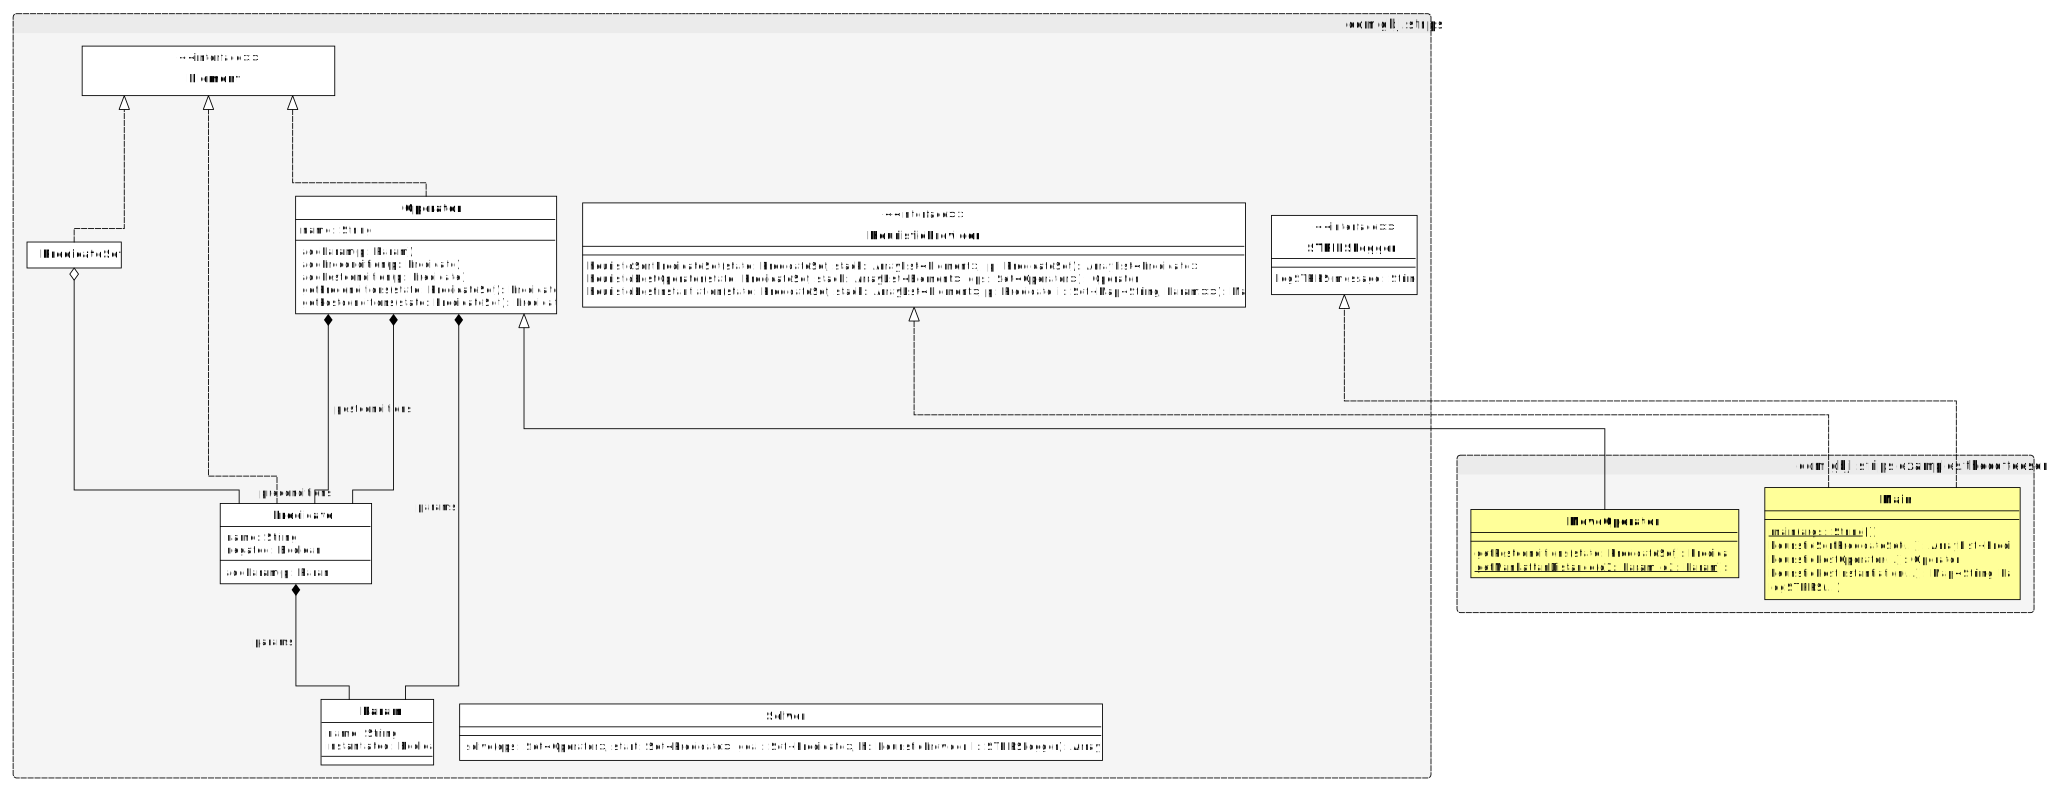
\includegraphics[scale=0.22]{simple}
	\end{center}
	\caption{Simple class diagram}
	\label{simplediagram}
\end{figure}

Package \texttt{com.gbjl.strips} contains the general STRIPS algorithm that, in summary, consists on these classes:
\begin{itemize}
	\item \texttt{Solver}: this class implements the STRIPS algorithm and it is executed when the method \texttt{solve(...)} is called with a given set of operators, an initial state, a goal state, a heuristic provider and a logger.
	\item \texttt{HeuristicProvider}: this interface provides the three heuristic functions that the solver uses, as explained in Section \ref{Planning Algorithm}. Class \texttt{Solver} calls those functions when needed.
	\item \texttt{STRIPSLogger}: this interface provides a function for logging messages. Class \texttt{Solver} calls this function several times to give information about what it is doing, as well as changes in the current state or the current stack.
	\item \texttt{Element}: this interface represents an element of the stack. In this simplification it has no methods, but internally it provides a function for the instantiation of parameters.
	\item \texttt{Param}: this class represents a parameter of a predicate or operator. It has a name and it can be instantiated (or not).
	\item \texttt{Predicate}: this class represents a predicate. It has a name, it can be negated (or not) and it contains a list of parameters.
	\item \texttt{Operator}: this class represents an operator. It has a name, a list of parameters, a list of preconditions and a list of postconditions. It can be extended with a subclass in order to implement advanced features, such as the \texttt{Move} operator of our coffee server problem, which requires a special case for managing the postcondition of \texttt{Steps(x+d)}.
	\item \texttt{PredicateSet}: this class represents a set of predicates.
\end{itemize}


Package \texttt{com.gbjl.strips.examples.thecoffeeserver} contains the particular case of the coffee server that consists on these classes:
\begin{itemize}
	\item \texttt{Main}: this class is the start point of the problem. It defines all the required operators (with its parameters, preconditions and postconditions), reads the initial and goal states from a given file and executes the STRIPS algorithm using \texttt{com.gbjs.strips.Solve}. It also provides the required heuristic functions and the logger function, that stores the algorithm log in a given file.
	\item \texttt{MoveOperator}: this class extends from \texttt{Operator}. It adds the required parameters, preconditions and postconditions to itself and overrides the \texttt{getPostconditions(...)} method, to be able to return the predicate \texttt{Steps(x+d)} based on the current state \texttt{Steps(x)} predicate. In order to simplify the problem, predicate \texttt{Steps(x)} has not been included in the list of preconditions of this operator, since it always exists in the current state.
\end{itemize}

\newpage
%----------------------------------------------------------------------------------------------------

\section{Results} \label{Results}

In this section we present and compare the results of several testing cases solved by our system:
\begin{itemize}
	\item Case 1: the example proposed in the problem definition. It consists on 5 petitions and 5 machines, and the proposal solves it with 25 steps.
	\item Case 2: a random example. It consists on 10 petitions and 10 machines.
	\item Case 3: another random example, but without a \texttt{Robot-location(o)} predicate in the goal state. It consists on 5 petitions and 5 machines.
	\item Case 4: a difficult case for our heuristic functions, that solve the problem in a very inefficient way. This is an example of a worst-case scenario for our solution: all petitions are distributed on two ends of the grid, and satisfy that all their suitable machines are located in their opposite end. We expect the robot to be constantly crossing without optimizing the travels at all.
	\item Case 5: an impossible case, where there is a petition of 1 coffees but no machines. It is expected that the program throws an error.
	\item Case 6: a random case with a lot of petitions (11) but few machines (3).
\end{itemize}
We point out that the exact input for each of these cases can be fount in Appendix C.

Table \ref{results} shows the performance of our algorithm measured in the number of steps the robot must do in order to achieve the goal state. This number is compared with the optimal solution, found using an algorithm not presented in this paper. Appendix C contains a detailed representation of the state and stack evolution of each execution of these tests.

% Please add the following required packages to your document preamble:
% \usepackage[table,xcdraw]{xcolor}
% If you use beamer only pass "xcolor=table" option, i.e. \documentclass[xcolor=table]{beamer}
\begin{table}[h!]
\centering
\begin{tabular}{|c|c|c|c|c|c|c|c|c|}
\hline
\textbf{Case} & \textbf{\begin{tabular}[c]{@{}c@{}}1 cup\\ petition\end{tabular}} & \textbf{\begin{tabular}[c]{@{}c@{}}2 cup\\ petition\end{tabular}} & \textbf{\begin{tabular}[c]{@{}c@{}}3 cup\\ petition\end{tabular}} & \textbf{\begin{tabular}[c]{@{}c@{}}1 cup\\ machines\end{tabular}} & \textbf{\begin{tabular}[c]{@{}c@{}}2 cup\\ machines\end{tabular}} & \textbf{\begin{tabular}[c]{@{}c@{}}3 cup\\ machines\end{tabular}} & \textbf{\begin{tabular}[c]{@{}c@{}}Final\\ steps\end{tabular}} & \textbf{\begin{tabular}[c]{@{}c@{}}Optimal\\ solution\end{tabular}} \\ \hline
1             & 3                                                                 & 1                                                                 & 1                                                                 & 2                                                                 & 2                                                                 & 1                                                                 & \cellcolor[HTML]{9AFF99}{\color[HTML]{333333} 25}              & 25                                                                  \\ \hline
2             & 6                                                                 & 2                                                                 & 2                                                                 & 2                                                                 & 2                                                                 & 6                                                                 & \cellcolor[HTML]{FFFC9E}56                                     & 52                                                                  \\ \hline
3             & 2                                                                 & 2                                                                 & 1                                                                 & 1                                                                 & 1                                                                 & 3                                                                 & \cellcolor[HTML]{FFFC9E}43                                     & 39                                                                  \\ \hline
4             & 1                                                                 & 1                                                                 & 1                                                                 & 1                                                                 & 1                                                                 & 1                                                                 & \cellcolor[HTML]{FFCCC9}42                                     & 26                                                                  \\ \hline
5             & 1                                                                 & 0                                                                 & 0                                                                 & 0                                                                 & 0                                                                 & 0                                                                 & N/A                                                            & N/A                                                                 \\ \hline
6             & 6                                                                 & 3                                                                 & 2                                                                 & 1                                                                 & 1                                                                 & 1                                                                 & \cellcolor[HTML]{FFFC9E}69                                     & 61                                                                  \\ \hline
\end{tabular}
\caption{Results of the different cases}
\label{results}
\end{table}

\newcommand{\plottwodee}[1]{
	\begin{tikzpicture}
		\begin{axis}[
				xlabel={#1},
				ylabel=Steps,
			]
			\addplot[
				scatter,
				only marks,
			]
			table[
				x=#1,
				y=Steps,
				col sep=comma,
			]{results.csv};
		\end{axis}		
	\end{tikzpicture}
}

In case 5, the program throws the following message:
\begin{listing}[style=consola, numbers=none]
Error. Predicate "Machine([o],1)" cannot be instantiated in the state "Petition(o1,1);Steps(0);Robot-free;Robot-location(o1);"
\end{listing}

In case 4, as we expected, we obtain the worst result by far. The robot, as we can see with much more detail in Appendix C, Case 4, instead of taking advantage of the crossings from one end to the other to serve the petitions of both sides at the same time, does respect the sequence of nearest petitions that the heuristic provides it and, consequently, delivers the petitions with a larger number of steps than required.


As the table shows, our solution is near the optimal solution for the major part of cases, but it is very inefficient for specific cases where the heuristic function do not sort the \texttt{Served(o)} predicates in a good way, since it does not take in account the position of the machines. However, this table is short and does not represents correctly the performance of our solution.


In order to have a better idea of the performance of the algorithm, we also created 300 random cases, where each case has a random number of machines between 1 and 36 and a random number of petitions between 1 and 36. All cases can be solved, since there exists a machine that makes N coffees for each petition of $N$ coffees.

Figures \ref{fig:2d-petitions}, \ref{fig:2d-petitions} and \ref{fig:3d-a} represent the relation between the number of petitions, the number of machines and the number of steps required to solve the problem.

In figure \ref{fig:2d-petitions} we can see how the number of petitions is directly correlated with the number of needed steps. Due to the low number of offices in the building, it is hard to determine the kind of correlation between both variables. However, from our point of view, it looks like an exponential function.
	
\begin{figure}[h!]
	\centering
	\plottwodee{Petitions}
	\caption{Relation between petitions and steps}
	\label{fig:2d-petitions}
\end{figure}

In \ref{fig:2d-petitions} we can see how the number of machines define a top limit to the number of needed steps. This limit is an inverse correlation between the two variables. Under this limit, the number of steps required to solve the problem does not follow any special distribution.

\begin{figure}[h!]
	\centering
	\plottwodee{Machines}
	\caption{Relation between machines and steps}
	\label{fig:2d-machines}
\end{figure}

\newcommand{\plotthreedee}[2]{
	\begin{axis}[
		view={#2}{#1},
		xlabel=Petitions,
		ylabel=Machines,
		zlabel=Steps,
	]
	\addplot3[
		scatter,
		only marks,
	]
	table[
		x=Petitions,
		y=Machines,
		z=Steps,
		col sep=comma,
	]{results.csv};
	\end{axis}
}

\clearpage

\begin{figure}
	\centering
	\begin{tikzpicture}
		\plotthreedee{20}{70}
	\end{tikzpicture}
	\caption{Relation between petitions, machines and steps (view A)}
\label{fig:3d-a}
\end{figure}

\begin{figure}
	\centering
	\begin{tikzpicture}
		\plotthreedee{45}{20}
	\end{tikzpicture}
	\caption{Relation between petitions, machines and steps (view B)}
	\label{fig:3d-a}
\end{figure}

\clearpage
%----------------------------------------------------------------------------------------------------

\section{Conclusions and Future Work} \label{Conclusions}

In sections \ref{Definition of the Problem} and \ref{Analysis of the Problem}, our team presented a definition of the problem and analyzed its characteristics, in order to formalize it as a set of operators and predicates to be able to solve it using the STRIPS algorithm.


Later, in section \ref{Planning Algorithm}, our team proposed several heuristic functions to optimize the result of the solver for this specific problem.


In section \ref{Implementation Design},  we presented a solution implemented in Java and we explained the details of the object oriented architecture.

Finally, a table of results was presented and analyzed, and we concluded that our solution is near to the optimal one, but in some cases can be very inefficient.


In general, due to the nature of the STRIPS algorithm, this program does not find the optimal plan for serving coffee with the minimum number of robot steps. Nevertheless, it can be close to it in many situations thanks to the proposed heuristic functions. Optimal solutions for this problem may be found using, for example, a non-linear planning algorithm with regression, but this subject is out of the scope of this paper.


\newpage
%--------------------------------------------------------------------------------------------------


%\thispagestyle{plain}
\begin{thebibliography}{25}
\addcontentsline{toc}{section}{References}\sectionmark{References}
	
	
	\bibitem{problemdefinition} PAR course. \textsl{MIA-MEISISI: Practical Exercise 1: Planner implementation}. Universitat Rovira i Virgili (URV), Tarragona, Spain, 2016. \url{https://moodle.urv.cat/moodle/pluginfile.php/2303642/mod_resource/content/4/PlannerExercise16-17.pdf}
	
	
	\bibitem{par} PAR course. \textsl{Guia docent 2016\_17}. Universitat Rovira i Virgili (URV), Tarragona, Spain, 2016. \url{https://moodle.urv.cat/docnet/guia_docent/index.php?centre=17&ensenyament=1768&assignatura=17685204&font=12&any_academic=2016_17&modalitat=p}
	
	
	\bibitem{strips} Richard E. Fikes and Nils J. Nilsson. \textsl{STRIPS: A New Approach to the
		Application of Theorem Proving to Problem Solving}. Stanford Research Institute, Menlo Park, California, 1971. \url{http://ai.stanford.edu/~nilsson/OnlinePubs-Nils/PublishedPapers/strips.pdf}
	
	
	\bibitem{java} Java programming language. \url{https://www.java.com/}
	
	
	\bibitem{gps} Ernst, G. and Newell, A. \textsl{GPS: A Case Study in Generality and Problem Solving}. ACM Monograph Series. Academic Press, New York, New York, 1969.
	
	
	\bibitem{notes} PAR course. \textsl{Lecture 3-3 Algorithm of the linear planner with a stack of objectives}. Universitat Rovira i Virgili (URV), Tarragona, Spain, 2016. \url{https://www.youtube.com/watch?v=8Zt3_EFdtPw}
	
\end{thebibliography}



%--------------------------------------------------------------------------------------------------
\newpage

\section*{Appendix A: Instructions to Execute the Program} \label{Instructions to Execute the Program}

\addcontentsline{toc}{section}{Appendix A: Instructions to Execute the Program}\sectionmark{Appendix A: Instructions to Execute the Program}

\subsection*{System requirements}
\begin{itemize}
	\item Microsoft Windows Vista or higher. (older versions are not supported by Microsoft\footnote{\url{https://support.microsoft.com/en-us/help/13853/windows-lifecycle-fact-sheet}} at the date of the publication of this paper).
	\item Java JDK 1.8\footnote{\url{http://www.oracle.com/technetwork/es/java/javase/downloads/index.html}}
\end{itemize}

\subsection*{Step 1: build}
In the command line console, go to the project directory and execute the following command:

\begin{listing}[style=consola, numbers=none]
build-thecoffeeserver.bat
\end{listing}

\subsection*{Step 2: run}
Now, to run the program, execute the following command:

\begin{listing}[style=consola, numbers=none]
java -jar out/thecoffeeserver.jar <input file> <output file>
\end{listing}
where:
\begin{itemize}
	\item \texttt{<input file>} is a file containing the initial and goal states, with the format stated in the problem definition.
	\item \texttt{<output file>} is the file where the program will store a detailed log of the solving process, including the plan (as a list of operators) to achieve the goal state from the initial state.
\end{itemize}

To run the input proposed in the problem definition, execute the following command:

\begin{listing}[style=consola, numbers=none]
java -jar out/thecoffeeserver.jar docs/thecoffeeserver/case1.txt out/output.txt
\end{listing}

The output of the program will be stored in out/output.txt.



%--------------------------------------------------------------------------------------------------
\newpage


\section*{Appendix B: Complete Class Diagram} \label{Complete Class Diagram}

\addcontentsline{toc}{section}{Appendix B: Complete Class Diagram}\sectionmark{Appendix B: Complete Class Diagram}

This is a complete class diagram of the system. Note that relation multiplicities have been omitted.

\begin{figure}[h!]
	\begin{center}
	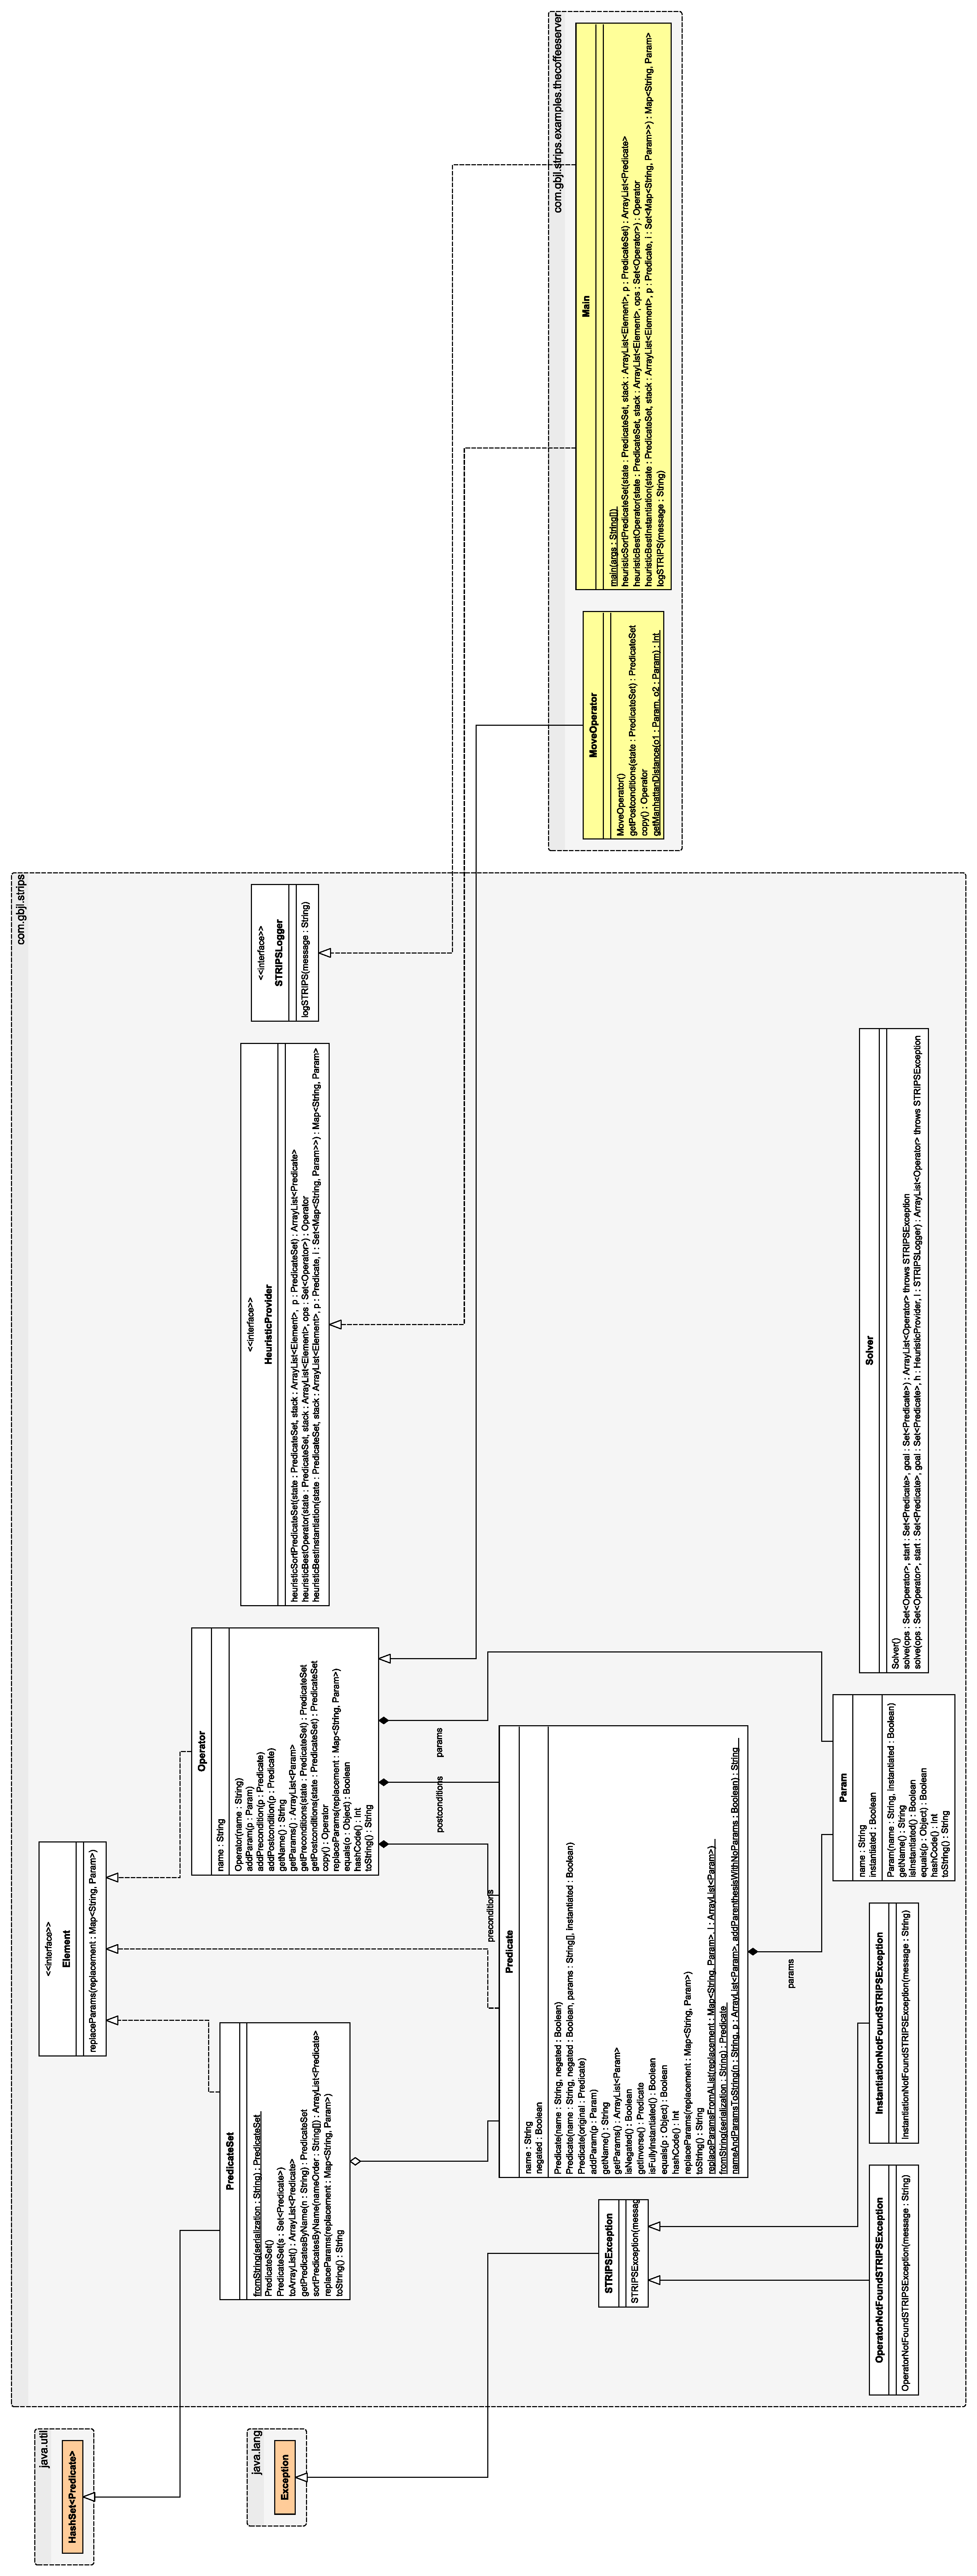
\includegraphics[scale=0.16]{gbjl-stripshor}
	\end{center}
	\caption{Complete class diagram}
\end{figure}

%--------------------------------------------------------------------------------------------------
\newpage

\section*{Appendix C: Test Results} \label{Test Results}

\addcontentsline{toc}{section}{Appendix C: Test Results}\sectionmark{Appendix C: Test Results}

This appendix contains a detailed representation of the state and stack evolution of each test execution proposed in Section \ref{Results}


For reasons of space, we abbreviated some predicates with the following dictionary:
\begin{itemize}
	\item Robot-loaded $\rightarrow$ RL
	\item Robot-free $\rightarrow$ RF
	\item Robot-location $\rightarrow$ R
	\item Steps $\rightarrow$ ST
	\item Machine $\rightarrow$ M
	\item Petition $\rightarrow$ P
	\item Served $\rightarrow$ S
\end{itemize}

For the same reason, when we represent a state using a 6x6 board with predicates in the corresponding cells, we omitted those parameters that reference office locations, since they are implicitly represented. For example, if \texttt{M(2)} is written in the cell (2,3) of a board, it means \texttt{Machine(o14,2)}.


\subsection*{Case 1}

\subsubsection*{Input File}

\begin{listing}[style=consola, numbers=none]
InitialState=Robot-location(o1);Machine(o4,3);Machine(o8,1);Machine(o21,2);Machine(o23,1);Machine(o31,2);Petition(o3,1); Petition(o11,3);Petition(o12,1);Petition(o13,2);Petition(o25,1);

GoalState=Robot-location(o7);Served(o3);Served(o11);Served(o12);Served(o13);Served(o25);
\end{listing}

\subsubsection{State evolution}

		\begin{multicols}{3}
		\centering
		\tiny
	

		\begin{tabular}[c]{@{}c@{}}
			\setlength\tabcolsep{3pt}
			\begin{tabular}{|c|c|c|c|c|c|}
				\hline
				\textcolor{blue}{R}	&		&	\textcolor{red}{P(1)}	&	\textcolor{brown}{M(3)}	&		&	 \\ \hline
					&	\textcolor{brown}{M(1)}	&		&		&	\textcolor{red}{P(3)}	&	\textcolor{red}{P(1)} \\ \hline
				\textcolor{red}{P(2)}	&		&		&		&		&	 \\ \hline
					&		&	\textcolor{brown}{M(2)}	&		&	\textcolor{brown}{M(1)}	&	 \\ \hline
				\textcolor{red}{P(1)}	&		&		&		&		&	 \\ \hline
				\textcolor{brown}{M(2)}	&		&		&		&		&	 \\ \hline
			\end{tabular}
			\\
			\\
			Robot-free; Steps(0)
			\\
			Initial state
			\\
			\\
			\\
		\end{tabular}
	


		\begin{tabular}[c]{@{}c@{}}
			\setlength\tabcolsep{3pt}
			\begin{tabular}{|c|c|c|c|c|c|}
				\hline
					&		&	\textcolor{red}{P(1)}	&	\textcolor{brown}{M(3)}	&		&	 \\ \hline
					&	\begin{tabular}[c]{@{}l@{}}\textcolor{blue}{R}\\\textcolor{brown}{M(1)}\end{tabular}	&		&		&	\textcolor{red}{P(3)}	&	\textcolor{red}{P(1)} \\ \hline
				\textcolor{red}{P(2)}	&		&		&		&		&	 \\ \hline
					&		&	\textcolor{brown}{M(2)}	&		&	\textcolor{brown}{M(1)}	&	 \\ \hline
				\textcolor{red}{P(1)}	&		&		&		&		&	 \\ \hline
				\textcolor{brown}{M(2)}	&		&		&		&		&	 \\ \hline
			\end{tabular}
			\\
			\\
			Robot-free; Steps(2)
			\\
			Intermediate state 1
			\\
			\\
			\\
		\end{tabular}
	


		\begin{tabular}[c]{@{}c@{}}
			\setlength\tabcolsep{3pt}
			\begin{tabular}{|c|c|c|c|c|c|}
				\hline
					&		&	\textcolor{red}{P(1)}	&	\textcolor{brown}{M(3)}	&		&	 \\ \hline
					&	\begin{tabular}[c]{@{}l@{}}\textcolor{blue}{R}\\\textcolor{brown}{M(1)}\end{tabular}	&		&		&	\textcolor{red}{P(3)}	&	\textcolor{red}{P(1)} \\ \hline
				\textcolor{red}{P(2)}	&		&		&		&		&	 \\ \hline
					&		&	\textcolor{brown}{M(2)}	&		&	\textcolor{brown}{M(1)}	&	 \\ \hline
				\textcolor{red}{P(1)}	&		&		&		&		&	 \\ \hline
				\textcolor{brown}{M(2)}	&		&		&		&		&	 \\ \hline
			\end{tabular}
			\\
			\\
			Robot-loaded(1); Steps(2)
			\\
			Intermediate state 2
			\\
			\\
			\\
		\end{tabular}
	


		\begin{tabular}[c]{@{}c@{}}
			\setlength\tabcolsep{3pt}
			\begin{tabular}{|c|c|c|c|c|c|}
				\hline
					&		&	\begin{tabular}[c]{@{}l@{}}\textcolor{red}{P(1)}\\\textcolor{blue}{R}\end{tabular}	&	\textcolor{brown}{M(3)}	&		&	 \\ \hline
					&	\textcolor{brown}{M(1)}	&		&		&	\textcolor{red}{P(3)}	&	\textcolor{red}{P(1)} \\ \hline
				\textcolor{red}{P(2)}	&		&		&		&		&	 \\ \hline
					&		&	\textcolor{brown}{M(2)}	&		&	\textcolor{brown}{M(1)}	&	 \\ \hline
				\textcolor{red}{P(1)}	&		&		&		&		&	 \\ \hline
				\textcolor{brown}{M(2)}	&		&		&		&		&	 \\ \hline
			\end{tabular}
			\\
			\\
			Robot-loaded(1); Steps(4)
			\\
			Intermediate state 3
			\\
			\\
			\\
		\end{tabular}
	


		\begin{tabular}[c]{@{}c@{}}
			\setlength\tabcolsep{3pt}
			\begin{tabular}{|c|c|c|c|c|c|}
				\hline
					&		&	\begin{tabular}[c]{@{}l@{}}\textcolor{blue}{R}\\\textcolor{green}{S}\end{tabular}	&	\textcolor{brown}{M(3)}	&		&	 \\ \hline
					&	\textcolor{brown}{M(1)}	&		&		&	\textcolor{red}{P(3)}	&	\textcolor{red}{P(1)} \\ \hline
				\textcolor{red}{P(2)}	&		&		&		&		&	 \\ \hline
					&		&	\textcolor{brown}{M(2)}	&		&	\textcolor{brown}{M(1)}	&	 \\ \hline
				\textcolor{red}{P(1)}	&		&		&		&		&	 \\ \hline
				\textcolor{brown}{M(2)}	&		&		&		&		&	 \\ \hline
			\end{tabular}
			\\
			\\
			Robot-free; Steps(4)
			\\
			Intermediate state 4
			\\
			\\
			\\
		\end{tabular}
	


		\begin{tabular}[c]{@{}c@{}}
			\setlength\tabcolsep{3pt}
			\begin{tabular}{|c|c|c|c|c|c|}
				\hline
					&		&	\textcolor{green}{S}	&	\begin{tabular}[c]{@{}l@{}}\textcolor{brown}{M(3)}\\\textcolor{blue}{R}\end{tabular}	&		&	 \\ \hline
					&	\textcolor{brown}{M(1)}	&		&		&	\textcolor{red}{P(3)}	&	\textcolor{red}{P(1)} \\ \hline
				\textcolor{red}{P(2)}	&		&		&		&		&	 \\ \hline
					&		&	\textcolor{brown}{M(2)}	&		&	\textcolor{brown}{M(1)}	&	 \\ \hline
				\textcolor{red}{P(1)}	&		&		&		&		&	 \\ \hline
				\textcolor{brown}{M(2)}	&		&		&		&		&	 \\ \hline
			\end{tabular}
			\\
			\\
			Robot-free; Steps(5)
			\\
			Intermediate state 5
			\\
			\\
			\\
		\end{tabular}
	


		\begin{tabular}[c]{@{}c@{}}
			\setlength\tabcolsep{3pt}
			\begin{tabular}{|c|c|c|c|c|c|}
				\hline
					&		&	\textcolor{green}{S}	&	\begin{tabular}[c]{@{}l@{}}\textcolor{brown}{M(3)}\\\textcolor{blue}{R}\end{tabular}	&		&	 \\ \hline
					&	\textcolor{brown}{M(1)}	&		&		&	\textcolor{red}{P(3)}	&	\textcolor{red}{P(1)} \\ \hline
				\textcolor{red}{P(2)}	&		&		&		&		&	 \\ \hline
					&		&	\textcolor{brown}{M(2)}	&		&	\textcolor{brown}{M(1)}	&	 \\ \hline
				\textcolor{red}{P(1)}	&		&		&		&		&	 \\ \hline
				\textcolor{brown}{M(2)}	&		&		&		&		&	 \\ \hline
			\end{tabular}
			\\
			\\
			Robot-loaded(3); Steps(5)
			\\
			Intermediate state 6
			\\
			\\
			\\
		\end{tabular}
	


		\begin{tabular}[c]{@{}c@{}}
			\setlength\tabcolsep{3pt}
			\begin{tabular}{|c|c|c|c|c|c|}
				\hline
					&		&	\textcolor{green}{S}	&	\textcolor{brown}{M(3)}	&		&	 \\ \hline
					&	\textcolor{brown}{M(1)}	&		&		&	\begin{tabular}[c]{@{}l@{}}\textcolor{blue}{R}\\\textcolor{red}{P(3)}\end{tabular}	&	\textcolor{red}{P(1)} \\ \hline
				\textcolor{red}{P(2)}	&		&		&		&		&	 \\ \hline
					&		&	\textcolor{brown}{M(2)}	&		&	\textcolor{brown}{M(1)}	&	 \\ \hline
				\textcolor{red}{P(1)}	&		&		&		&		&	 \\ \hline
				\textcolor{brown}{M(2)}	&		&		&		&		&	 \\ \hline
			\end{tabular}
			\\
			\\
			Robot-loaded(3); Steps(7)
			\\
			Intermediate state 7
			\\
			\\
			\\
		\end{tabular}
	


		\begin{tabular}[c]{@{}c@{}}
			\setlength\tabcolsep{3pt}
			\begin{tabular}{|c|c|c|c|c|c|}
				\hline
					&		&	\textcolor{green}{S}	&	\textcolor{brown}{M(3)}	&		&	 \\ \hline
					&	\textcolor{brown}{M(1)}	&		&		&	\begin{tabular}[c]{@{}l@{}}\textcolor{green}{S}\\\textcolor{blue}{R}\end{tabular}	&	\textcolor{red}{P(1)} \\ \hline
				\textcolor{red}{P(2)}	&		&		&		&		&	 \\ \hline
					&		&	\textcolor{brown}{M(2)}	&		&	\textcolor{brown}{M(1)}	&	 \\ \hline
				\textcolor{red}{P(1)}	&		&		&		&		&	 \\ \hline
				\textcolor{brown}{M(2)}	&		&		&		&		&	 \\ \hline
			\end{tabular}
			\\
			\\
			Robot-free; Steps(7)
			\\
			Intermediate state 8
			\\
			\\
			\\
		\end{tabular}
	


		\begin{tabular}[c]{@{}c@{}}
			\setlength\tabcolsep{3pt}
			\begin{tabular}{|c|c|c|c|c|c|}
				\hline
					&		&	\textcolor{green}{S}	&	\textcolor{brown}{M(3)}	&		&	 \\ \hline
					&	\textcolor{brown}{M(1)}	&		&		&	\textcolor{green}{S}	&	\textcolor{red}{P(1)} \\ \hline
				\textcolor{red}{P(2)}	&		&		&		&		&	 \\ \hline
					&		&	\textcolor{brown}{M(2)}	&		&	\begin{tabular}[c]{@{}l@{}}\textcolor{brown}{M(1)}\\\textcolor{blue}{R}\end{tabular}	&	 \\ \hline
				\textcolor{red}{P(1)}	&		&		&		&		&	 \\ \hline
				\textcolor{brown}{M(2)}	&		&		&		&		&	 \\ \hline
			\end{tabular}
			\\
			\\
			Robot-free; Steps(9)
			\\
			Intermediate state 9
			\\
			\\
			\\
		\end{tabular}
	


		\begin{tabular}[c]{@{}c@{}}
			\setlength\tabcolsep{3pt}
			\begin{tabular}{|c|c|c|c|c|c|}
				\hline
					&		&	\textcolor{green}{S}	&	\textcolor{brown}{M(3)}	&		&	 \\ \hline
					&	\textcolor{brown}{M(1)}	&		&		&	\textcolor{green}{S}	&	\textcolor{red}{P(1)} \\ \hline
				\textcolor{red}{P(2)}	&		&		&		&		&	 \\ \hline
					&		&	\textcolor{brown}{M(2)}	&		&	\begin{tabular}[c]{@{}l@{}}\textcolor{brown}{M(1)}\\\textcolor{blue}{R}\end{tabular}	&	 \\ \hline
				\textcolor{red}{P(1)}	&		&		&		&		&	 \\ \hline
				\textcolor{brown}{M(2)}	&		&		&		&		&	 \\ \hline
			\end{tabular}
			\\
			\\
			Robot-loaded(1); Steps(9)
			\\
			Intermediate state 10
			\\
			\\
			\\
		\end{tabular}
	


		\begin{tabular}[c]{@{}c@{}}
			\setlength\tabcolsep{3pt}
			\begin{tabular}{|c|c|c|c|c|c|}
				\hline
					&		&	\textcolor{green}{S}	&	\textcolor{brown}{M(3)}	&		&	 \\ \hline
					&	\textcolor{brown}{M(1)}	&		&		&	\textcolor{green}{S}	&	\begin{tabular}[c]{@{}l@{}}\textcolor{red}{P(1)}\\\textcolor{blue}{R}\end{tabular} \\ \hline
				\textcolor{red}{P(2)}	&		&		&		&		&	 \\ \hline
					&		&	\textcolor{brown}{M(2)}	&		&	\textcolor{brown}{M(1)}	&	 \\ \hline
				\textcolor{red}{P(1)}	&		&		&		&		&	 \\ \hline
				\textcolor{brown}{M(2)}	&		&		&		&		&	 \\ \hline
			\end{tabular}
			\\
			\\
			Robot-loaded(1); Steps(12)
			\\
			Intermediate state 11
			\\
			\\
			\\
		\end{tabular}
	


		\begin{tabular}[c]{@{}c@{}}
			\setlength\tabcolsep{3pt}
			\begin{tabular}{|c|c|c|c|c|c|}
				\hline
					&		&	\textcolor{green}{S}	&	\textcolor{brown}{M(3)}	&		&	 \\ \hline
					&	\textcolor{brown}{M(1)}	&		&		&	\textcolor{green}{S}	&	\begin{tabular}[c]{@{}l@{}}\textcolor{green}{S}\\\textcolor{blue}{R}\end{tabular} \\ \hline
				\textcolor{red}{P(2)}	&		&		&		&		&	 \\ \hline
					&		&	\textcolor{brown}{M(2)}	&		&	\textcolor{brown}{M(1)}	&	 \\ \hline
				\textcolor{red}{P(1)}	&		&		&		&		&	 \\ \hline
				\textcolor{brown}{M(2)}	&		&		&		&		&	 \\ \hline
			\end{tabular}
			\\
			\\
			Robot-free; Steps(12)
			\\
			Intermediate state 12
			\\
			\\
			\\
		\end{tabular}
	


		\begin{tabular}[c]{@{}c@{}}
			\setlength\tabcolsep{3pt}
			\begin{tabular}{|c|c|c|c|c|c|}
				\hline
					&		&	\textcolor{green}{S}	&	\textcolor{brown}{M(3)}	&		&	 \\ \hline
					&	\textcolor{brown}{M(1)}	&		&		&	\textcolor{green}{S}	&	\textcolor{green}{S} \\ \hline
				\textcolor{red}{P(2)}	&		&		&		&		&	 \\ \hline
					&		&	\textcolor{brown}{M(2)}	&		&	\begin{tabular}[c]{@{}l@{}}\textcolor{brown}{M(1)}\\\textcolor{blue}{R}\end{tabular}	&	 \\ \hline
				\textcolor{red}{P(1)}	&		&		&		&		&	 \\ \hline
				\textcolor{brown}{M(2)}	&		&		&		&		&	 \\ \hline
			\end{tabular}
			\\
			\\
			Robot-free; Steps(15)
			\\
			Intermediate state 13
			\\
			\\
			\\
		\end{tabular}
	


		\begin{tabular}[c]{@{}c@{}}
			\setlength\tabcolsep{3pt}
			\begin{tabular}{|c|c|c|c|c|c|}
				\hline
					&		&	\textcolor{green}{S}	&	\textcolor{brown}{M(3)}	&		&	 \\ \hline
					&	\textcolor{brown}{M(1)}	&		&		&	\textcolor{green}{S}	&	\textcolor{green}{S} \\ \hline
				\textcolor{red}{P(2)}	&		&		&		&		&	 \\ \hline
					&		&	\textcolor{brown}{M(2)}	&		&	\begin{tabular}[c]{@{}l@{}}\textcolor{brown}{M(1)}\\\textcolor{blue}{R}\end{tabular}	&	 \\ \hline
				\textcolor{red}{P(1)}	&		&		&		&		&	 \\ \hline
				\textcolor{brown}{M(2)}	&		&		&		&		&	 \\ \hline
			\end{tabular}
			\\
			\\
			Robot-loaded(1); Steps(15)
			\\
			Intermediate state 14
			\\
			\\
			\\
		\end{tabular}
	


		\begin{tabular}[c]{@{}c@{}}
			\setlength\tabcolsep{3pt}
			\begin{tabular}{|c|c|c|c|c|c|}
				\hline
					&		&	\textcolor{green}{S}	&	\textcolor{brown}{M(3)}	&		&	 \\ \hline
					&	\textcolor{brown}{M(1)}	&		&		&	\textcolor{green}{S}	&	\textcolor{green}{S} \\ \hline
				\textcolor{red}{P(2)}	&		&		&		&		&	 \\ \hline
					&		&	\textcolor{brown}{M(2)}	&		&	\textcolor{brown}{M(1)}	&	 \\ \hline
				\begin{tabular}[c]{@{}l@{}}\textcolor{blue}{R}\\\textcolor{red}{P(1)}\end{tabular}	&		&		&		&		&	 \\ \hline
				\textcolor{brown}{M(2)}	&		&		&		&		&	 \\ \hline
			\end{tabular}
			\\
			\\
			Robot-loaded(1); Steps(20)
			\\
			Intermediate state 15
			\\
			\\
			\\
		\end{tabular}
	


		\begin{tabular}[c]{@{}c@{}}
			\setlength\tabcolsep{3pt}
			\begin{tabular}{|c|c|c|c|c|c|}
				\hline
					&		&	\textcolor{green}{S}	&	\textcolor{brown}{M(3)}	&		&	 \\ \hline
					&	\textcolor{brown}{M(1)}	&		&		&	\textcolor{green}{S}	&	\textcolor{green}{S} \\ \hline
				\textcolor{red}{P(2)}	&		&		&		&		&	 \\ \hline
					&		&	\textcolor{brown}{M(2)}	&		&	\textcolor{brown}{M(1)}	&	 \\ \hline
				\begin{tabular}[c]{@{}l@{}}\textcolor{blue}{R}\\\textcolor{green}{S}\end{tabular}	&		&		&		&		&	 \\ \hline
				\textcolor{brown}{M(2)}	&		&		&		&		&	 \\ \hline
			\end{tabular}
			\\
			\\
			Robot-free; Steps(20)
			\\
			Intermediate state 16
			\\
			\\
			\\
		\end{tabular}
	


		\begin{tabular}[c]{@{}c@{}}
			\setlength\tabcolsep{3pt}
			\begin{tabular}{|c|c|c|c|c|c|}
				\hline
					&		&	\textcolor{green}{S}	&	\textcolor{brown}{M(3)}	&		&	 \\ \hline
					&	\textcolor{brown}{M(1)}	&		&		&	\textcolor{green}{S}	&	\textcolor{green}{S} \\ \hline
				\textcolor{red}{P(2)}	&		&		&		&		&	 \\ \hline
					&		&	\textcolor{brown}{M(2)}	&		&	\textcolor{brown}{M(1)}	&	 \\ \hline
				\textcolor{green}{S}	&		&		&		&		&	 \\ \hline
				\begin{tabular}[c]{@{}l@{}}\textcolor{blue}{R}\\\textcolor{brown}{M(2)}\end{tabular}	&		&		&		&		&	 \\ \hline
			\end{tabular}
			\\
			\\
			Robot-free; Steps(21)
			\\
			Intermediate state 17
			\\
			\\
			\\
		\end{tabular}
	


		\begin{tabular}[c]{@{}c@{}}
			\setlength\tabcolsep{3pt}
			\begin{tabular}{|c|c|c|c|c|c|}
				\hline
					&		&	\textcolor{green}{S}	&	\textcolor{brown}{M(3)}	&		&	 \\ \hline
					&	\textcolor{brown}{M(1)}	&		&		&	\textcolor{green}{S}	&	\textcolor{green}{S} \\ \hline
				\textcolor{red}{P(2)}	&		&		&		&		&	 \\ \hline
					&		&	\textcolor{brown}{M(2)}	&		&	\textcolor{brown}{M(1)}	&	 \\ \hline
				\textcolor{green}{S}	&		&		&		&		&	 \\ \hline
				\begin{tabular}[c]{@{}l@{}}\textcolor{blue}{R}\\\textcolor{brown}{M(2)}\end{tabular}	&		&		&		&		&	 \\ \hline
			\end{tabular}
			\\
			\\
			Robot-loaded(2); Steps(21)
			\\
			Intermediate state 18
			\\
			\\
			\\
		\end{tabular}
	


		\begin{tabular}[c]{@{}c@{}}
			\setlength\tabcolsep{3pt}
			\begin{tabular}{|c|c|c|c|c|c|}
				\hline
					&		&	\textcolor{green}{S}	&	\textcolor{brown}{M(3)}	&		&	 \\ \hline
					&	\textcolor{brown}{M(1)}	&		&		&	\textcolor{green}{S}	&	\textcolor{green}{S} \\ \hline
				\begin{tabular}[c]{@{}l@{}}\textcolor{blue}{R}\\\textcolor{red}{P(2)}\end{tabular}	&		&		&		&		&	 \\ \hline
					&		&	\textcolor{brown}{M(2)}	&		&	\textcolor{brown}{M(1)}	&	 \\ \hline
				\textcolor{green}{S}	&		&		&		&		&	 \\ \hline
				\textcolor{brown}{M(2)}	&		&		&		&		&	 \\ \hline
			\end{tabular}
			\\
			\\
			Robot-loaded(2); Steps(24)
			\\
			Intermediate state 19
			\\
			\\
			\\
		\end{tabular}
	


		\begin{tabular}[c]{@{}c@{}}
			\setlength\tabcolsep{3pt}
			\begin{tabular}{|c|c|c|c|c|c|}
				\hline
					&		&	\textcolor{green}{S}	&	\textcolor{brown}{M(3)}	&		&	 \\ \hline
					&	\textcolor{brown}{M(1)}	&		&		&	\textcolor{green}{S}	&	\textcolor{green}{S} \\ \hline
				\begin{tabular}[c]{@{}l@{}}\textcolor{green}{S}\\\textcolor{blue}{R}\end{tabular}	&		&		&		&		&	 \\ \hline
					&		&	\textcolor{brown}{M(2)}	&		&	\textcolor{brown}{M(1)}	&	 \\ \hline
				\textcolor{green}{S}	&		&		&		&		&	 \\ \hline
				\textcolor{brown}{M(2)}	&		&		&		&		&	 \\ \hline
			\end{tabular}
			\\
			\\
			Robot-free; Steps(24)
			\\
			Intermediate state 20
			\\
			\\
			\\
		\end{tabular}
	


		\begin{tabular}[c]{@{}c@{}}
			\setlength\tabcolsep{3pt}
			\begin{tabular}{|c|c|c|c|c|c|}
				\hline
					&		&	\textcolor{green}{S}	&	\textcolor{brown}{M(3)}	&		&	 \\ \hline
				\textcolor{blue}{R}	&	\textcolor{brown}{M(1)}	&		&		&	\textcolor{green}{S}	&	\textcolor{green}{S} \\ \hline
				\textcolor{green}{S}	&		&		&		&		&	 \\ \hline
					&		&	\textcolor{brown}{M(2)}	&		&	\textcolor{brown}{M(1)}	&	 \\ \hline
				\textcolor{green}{S}	&		&		&		&		&	 \\ \hline
				\textcolor{brown}{M(2)}	&		&		&		&		&	 \\ \hline
			\end{tabular}
			\\
			\\
			Robot-free; Steps(25)
			\\
			Final state
			\\
			\\
			\\
		\end{tabular}
	


		\begin{tabular}[c]{@{}c@{}}
			\setlength\tabcolsep{3pt}
			\begin{tabular}{|c|c|c|c|c|c|}
				\hline
					&		&	\textcolor{green}{S}	&		&		&	 \\ \hline
				\textcolor{blue}{R}	&		&		&		&	\textcolor{green}{S}	&	\textcolor{green}{S} \\ \hline
				\textcolor{green}{S}	&		&		&		&		&	 \\ \hline
					&		&		&		&		&	 \\ \hline
				\textcolor{green}{S}	&		&		&		&		&	 \\ \hline
					&		&		&		&		&	 \\ \hline
			\end{tabular}
			\\
			\\
			
			\\
			Goal state
			\\
			\\
			\\
		\end{tabular}
	

		\end{multicols}
	
\subsubsection{Stack evolution}

		\begin{multicols}{3}
		\centering
		\tiny
	

		\begin{tabular}[c]{@{}c@{}}
			\setlength\tabcolsep{3pt}
			\begin{tabular}{|c|}
				\hline
				Served(o3) \\ \hline
				Served(o11) \\ \hline
				Served(o12) \\ \hline
				Served(o25) \\ \hline
				Served(o13) \\ \hline
				Robot-location(o7) \\ \hline
				\{S(o3), S(o12), S(o13), S(o25), R(o7), S(o11)\} \\ \hline
			\end{tabular}
			\\
			\\
			Stack \#1
			\\
			\\
			\\
		\end{tabular}
	


		\begin{tabular}[c]{@{}c@{}}
			\setlength\tabcolsep{3pt}
			\begin{tabular}{|c|}
				\hline
				Petition(o3,[n]) \\ \hline
				Robot-loaded([n]) \\ \hline
				Robot-location(o3) \\ \hline
				\{R(o3), RL([n]), P(o3,[n])\} \\ \hline
				Serve(o3,[n]) \\ \hline
				Served(o11) \\ \hline
				Served(o12) \\ \hline
				Served(o25) \\ \hline
				Served(o13) \\ \hline
				Robot-location(o7) \\ \hline
				\{S(o3), S(o12), S(o13), S(o25), R(o7), S(o11)\} \\ \hline
			\end{tabular}
			\\
			\\
			Stack \#2
			\\
			\\
			\\
		\end{tabular}
	


		\begin{tabular}[c]{@{}c@{}}
			\setlength\tabcolsep{3pt}
			\begin{tabular}{|c|}
				\hline
				Robot-loaded(1) \\ \hline
				Robot-location(o3) \\ \hline
				\{R(o3), RL(1), P(o3,1)\} \\ \hline
				Serve(o3,1) \\ \hline
				Served(o11) \\ \hline
				Served(o12) \\ \hline
				Served(o25) \\ \hline
				Served(o13) \\ \hline
				Robot-location(o7) \\ \hline
				\{S(o3), S(o12), S(o13), S(o25), R(o7), S(o11)\} \\ \hline
			\end{tabular}
			\\
			\\
			Stack \#3
			\\
			\\
			\\
		\end{tabular}
	


		\begin{tabular}[c]{@{}c@{}}
			\setlength\tabcolsep{3pt}
			\begin{tabular}{|c|}
				\hline
				Robot-free \\ \hline
				Machine([o],1) \\ \hline
				Robot-location([o]) \\ \hline
				\{M([o],1), R([o]), RF\} \\ \hline
				Make([o],1) \\ \hline
				Robot-location(o3) \\ \hline
				\{R(o3), RL(1), P(o3,1)\} \\ \hline
				Serve(o3,1) \\ \hline
				Served(o11) \\ \hline
				Served(o12) \\ \hline
				Served(o25) \\ \hline
				Served(o13) \\ \hline
				Robot-location(o7) \\ \hline
				\{S(o3), S(o12), S(o13), S(o25), R(o7), S(o11)\} \\ \hline
			\end{tabular}
			\\
			\\
			Stack \#4
			\\
			\\
			\\
		\end{tabular}
	


		\begin{tabular}[c]{@{}c@{}}
			\setlength\tabcolsep{3pt}
			\begin{tabular}{|c|}
				\hline
				Machine([o],1) \\ \hline
				Robot-location([o]) \\ \hline
				\{M([o],1), R([o]), RF\} \\ \hline
				Make([o],1) \\ \hline
				Robot-location(o3) \\ \hline
				\{R(o3), RL(1), P(o3,1)\} \\ \hline
				Serve(o3,1) \\ \hline
				Served(o11) \\ \hline
				Served(o12) \\ \hline
				Served(o25) \\ \hline
				Served(o13) \\ \hline
				Robot-location(o7) \\ \hline
				\{S(o3), S(o12), S(o13), S(o25), R(o7), S(o11)\} \\ \hline
			\end{tabular}
			\\
			\\
			Stack \#5
			\\
			\\
			\\
		\end{tabular}
	


		\begin{tabular}[c]{@{}c@{}}
			\setlength\tabcolsep{3pt}
			\begin{tabular}{|c|}
				\hline
				Robot-location(o8) \\ \hline
				\{M(o8,1), R(o8), RF\} \\ \hline
				Make(o8,1) \\ \hline
				Robot-location(o3) \\ \hline
				\{R(o3), RL(1), P(o3,1)\} \\ \hline
				Serve(o3,1) \\ \hline
				Served(o11) \\ \hline
				Served(o12) \\ \hline
				Served(o25) \\ \hline
				Served(o13) \\ \hline
				Robot-location(o7) \\ \hline
				\{S(o3), S(o12), S(o13), S(o25), R(o7), S(o11)\} \\ \hline
			\end{tabular}
			\\
			\\
			Stack \#6
			\\
			\\
			\\
		\end{tabular}
	


		\begin{tabular}[c]{@{}c@{}}
			\setlength\tabcolsep{3pt}
			\begin{tabular}{|c|}
				\hline
				Robot-location([o1]) \\ \hline
				\{R([o1])\} \\ \hline
				Move([o1],o8) \\ \hline
				\{M(o8,1), R(o8), RF\} \\ \hline
				Make(o8,1) \\ \hline
				Robot-location(o3) \\ \hline
				\{R(o3), RL(1), P(o3,1)\} \\ \hline
				Serve(o3,1) \\ \hline
				Served(o11) \\ \hline
				Served(o12) \\ \hline
				Served(o25) \\ \hline
				Served(o13) \\ \hline
				Robot-location(o7) \\ \hline
				\{S(o3), S(o12), S(o13), S(o25), R(o7), S(o11)\} \\ \hline
			\end{tabular}
			\\
			\\
			Stack \#7
			\\
			\\
			\\
		\end{tabular}
	


		\begin{tabular}[c]{@{}c@{}}
			\setlength\tabcolsep{3pt}
			\begin{tabular}{|c|}
				\hline
				\{R(o1)\} \\ \hline
				Move(o1,o8) \\ \hline
				\{M(o8,1), R(o8), RF\} \\ \hline
				Make(o8,1) \\ \hline
				Robot-location(o3) \\ \hline
				\{R(o3), RL(1), P(o3,1)\} \\ \hline
				Serve(o3,1) \\ \hline
				Served(o11) \\ \hline
				Served(o12) \\ \hline
				Served(o25) \\ \hline
				Served(o13) \\ \hline
				Robot-location(o7) \\ \hline
				\{S(o3), S(o12), S(o13), S(o25), R(o7), S(o11)\} \\ \hline
			\end{tabular}
			\\
			\\
			Stack \#8
			\\
			\\
			\\
		\end{tabular}
	


		\begin{tabular}[c]{@{}c@{}}
			\setlength\tabcolsep{3pt}
			\begin{tabular}{|c|}
				\hline
				Move(o1,o8) \\ \hline
				\{M(o8,1), R(o8), RF\} \\ \hline
				Make(o8,1) \\ \hline
				Robot-location(o3) \\ \hline
				\{R(o3), RL(1), P(o3,1)\} \\ \hline
				Serve(o3,1) \\ \hline
				Served(o11) \\ \hline
				Served(o12) \\ \hline
				Served(o25) \\ \hline
				Served(o13) \\ \hline
				Robot-location(o7) \\ \hline
				\{S(o3), S(o12), S(o13), S(o25), R(o7), S(o11)\} \\ \hline
			\end{tabular}
			\\
			\\
			Stack \#9
			\\
			\\
			\\
		\end{tabular}
	


		\begin{tabular}[c]{@{}c@{}}
			\setlength\tabcolsep{3pt}
			\begin{tabular}{|c|}
				\hline
				\{M(o8,1), R(o8), RF\} \\ \hline
				Make(o8,1) \\ \hline
				Robot-location(o3) \\ \hline
				\{R(o3), RL(1), P(o3,1)\} \\ \hline
				Serve(o3,1) \\ \hline
				Served(o11) \\ \hline
				Served(o12) \\ \hline
				Served(o25) \\ \hline
				Served(o13) \\ \hline
				Robot-location(o7) \\ \hline
				\{S(o3), S(o12), S(o13), S(o25), R(o7), S(o11)\} \\ \hline
			\end{tabular}
			\\
			\\
			Stack \#10
			\\
			\\
			\\
		\end{tabular}
	


		\begin{tabular}[c]{@{}c@{}}
			\setlength\tabcolsep{3pt}
			\begin{tabular}{|c|}
				\hline
				Make(o8,1) \\ \hline
				Robot-location(o3) \\ \hline
				\{R(o3), RL(1), P(o3,1)\} \\ \hline
				Serve(o3,1) \\ \hline
				Served(o11) \\ \hline
				Served(o12) \\ \hline
				Served(o25) \\ \hline
				Served(o13) \\ \hline
				Robot-location(o7) \\ \hline
				\{S(o3), S(o12), S(o13), S(o25), R(o7), S(o11)\} \\ \hline
			\end{tabular}
			\\
			\\
			Stack \#11
			\\
			\\
			\\
		\end{tabular}
	


		\begin{tabular}[c]{@{}c@{}}
			\setlength\tabcolsep{3pt}
			\begin{tabular}{|c|}
				\hline
				Robot-location(o3) \\ \hline
				\{R(o3), RL(1), P(o3,1)\} \\ \hline
				Serve(o3,1) \\ \hline
				Served(o11) \\ \hline
				Served(o12) \\ \hline
				Served(o25) \\ \hline
				Served(o13) \\ \hline
				Robot-location(o7) \\ \hline
				\{S(o3), S(o12), S(o13), S(o25), R(o7), S(o11)\} \\ \hline
			\end{tabular}
			\\
			\\
			Stack \#12
			\\
			\\
			\\
		\end{tabular}
	


		\begin{tabular}[c]{@{}c@{}}
			\setlength\tabcolsep{3pt}
			\begin{tabular}{|c|}
				\hline
				Robot-location([o1]) \\ \hline
				\{R([o1])\} \\ \hline
				Move([o1],o3) \\ \hline
				\{R(o3), RL(1), P(o3,1)\} \\ \hline
				Serve(o3,1) \\ \hline
				Served(o11) \\ \hline
				Served(o12) \\ \hline
				Served(o25) \\ \hline
				Served(o13) \\ \hline
				Robot-location(o7) \\ \hline
				\{S(o3), S(o12), S(o13), S(o25), R(o7), S(o11)\} \\ \hline
			\end{tabular}
			\\
			\\
			Stack \#13
			\\
			\\
			\\
		\end{tabular}
	


		\begin{tabular}[c]{@{}c@{}}
			\setlength\tabcolsep{3pt}
			\begin{tabular}{|c|}
				\hline
				\{R(o8)\} \\ \hline
				Move(o8,o3) \\ \hline
				\{R(o3), RL(1), P(o3,1)\} \\ \hline
				Serve(o3,1) \\ \hline
				Served(o11) \\ \hline
				Served(o12) \\ \hline
				Served(o25) \\ \hline
				Served(o13) \\ \hline
				Robot-location(o7) \\ \hline
				\{S(o3), S(o12), S(o13), S(o25), R(o7), S(o11)\} \\ \hline
			\end{tabular}
			\\
			\\
			Stack \#14
			\\
			\\
			\\
		\end{tabular}
	


		\begin{tabular}[c]{@{}c@{}}
			\setlength\tabcolsep{3pt}
			\begin{tabular}{|c|}
				\hline
				Move(o8,o3) \\ \hline
				\{R(o3), RL(1), P(o3,1)\} \\ \hline
				Serve(o3,1) \\ \hline
				Served(o11) \\ \hline
				Served(o12) \\ \hline
				Served(o25) \\ \hline
				Served(o13) \\ \hline
				Robot-location(o7) \\ \hline
				\{S(o3), S(o12), S(o13), S(o25), R(o7), S(o11)\} \\ \hline
			\end{tabular}
			\\
			\\
			Stack \#15
			\\
			\\
			\\
		\end{tabular}
	


		\begin{tabular}[c]{@{}c@{}}
			\setlength\tabcolsep{3pt}
			\begin{tabular}{|c|}
				\hline
				\{R(o3), RL(1), P(o3,1)\} \\ \hline
				Serve(o3,1) \\ \hline
				Served(o11) \\ \hline
				Served(o12) \\ \hline
				Served(o25) \\ \hline
				Served(o13) \\ \hline
				Robot-location(o7) \\ \hline
				\{S(o3), S(o12), S(o13), S(o25), R(o7), S(o11)\} \\ \hline
			\end{tabular}
			\\
			\\
			Stack \#16
			\\
			\\
			\\
		\end{tabular}
	


		\begin{tabular}[c]{@{}c@{}}
			\setlength\tabcolsep{3pt}
			\begin{tabular}{|c|}
				\hline
				Serve(o3,1) \\ \hline
				Served(o11) \\ \hline
				Served(o12) \\ \hline
				Served(o25) \\ \hline
				Served(o13) \\ \hline
				Robot-location(o7) \\ \hline
				\{S(o3), S(o12), S(o13), S(o25), R(o7), S(o11)\} \\ \hline
			\end{tabular}
			\\
			\\
			Stack \#17
			\\
			\\
			\\
		\end{tabular}
	


		\begin{tabular}[c]{@{}c@{}}
			\setlength\tabcolsep{3pt}
			\begin{tabular}{|c|}
				\hline
				Served(o11) \\ \hline
				Served(o12) \\ \hline
				Served(o25) \\ \hline
				Served(o13) \\ \hline
				Robot-location(o7) \\ \hline
				\{S(o3), S(o12), S(o13), S(o25), R(o7), S(o11)\} \\ \hline
			\end{tabular}
			\\
			\\
			Stack \#18
			\\
			\\
			\\
		\end{tabular}
	


		\begin{tabular}[c]{@{}c@{}}
			\setlength\tabcolsep{3pt}
			\begin{tabular}{|c|}
				\hline
				Petition(o11,[n]) \\ \hline
				Robot-loaded([n]) \\ \hline
				Robot-location(o11) \\ \hline
				\{R(o11), RL([n]), P(o11,[n])\} \\ \hline
				Serve(o11,[n]) \\ \hline
				Served(o12) \\ \hline
				Served(o25) \\ \hline
				Served(o13) \\ \hline
				Robot-location(o7) \\ \hline
				\{S(o3), S(o12), S(o13), S(o25), R(o7), S(o11)\} \\ \hline
			\end{tabular}
			\\
			\\
			Stack \#19
			\\
			\\
			\\
		\end{tabular}
	


		\begin{tabular}[c]{@{}c@{}}
			\setlength\tabcolsep{3pt}
			\begin{tabular}{|c|}
				\hline
				Robot-loaded(3) \\ \hline
				Robot-location(o11) \\ \hline
				\{R(o11), RL(3), P(o11,3)\} \\ \hline
				Serve(o11,3) \\ \hline
				Served(o12) \\ \hline
				Served(o25) \\ \hline
				Served(o13) \\ \hline
				Robot-location(o7) \\ \hline
				\{S(o3), S(o12), S(o13), S(o25), R(o7), S(o11)\} \\ \hline
			\end{tabular}
			\\
			\\
			Stack \#20
			\\
			\\
			\\
		\end{tabular}
	


		\begin{tabular}[c]{@{}c@{}}
			\setlength\tabcolsep{3pt}
			\begin{tabular}{|c|}
				\hline
				Robot-free \\ \hline
				Machine([o],3) \\ \hline
				Robot-location([o]) \\ \hline
				\{R([o]), RF, M([o],3)\} \\ \hline
				Make([o],3) \\ \hline
				Robot-location(o11) \\ \hline
				\{R(o11), RL(3), P(o11,3)\} \\ \hline
				Serve(o11,3) \\ \hline
				Served(o12) \\ \hline
				Served(o25) \\ \hline
				Served(o13) \\ \hline
				Robot-location(o7) \\ \hline
				\{S(o3), S(o12), S(o13), S(o25), R(o7), S(o11)\} \\ \hline
			\end{tabular}
			\\
			\\
			Stack \#21
			\\
			\\
			\\
		\end{tabular}
	


		\begin{tabular}[c]{@{}c@{}}
			\setlength\tabcolsep{3pt}
			\begin{tabular}{|c|}
				\hline
				Machine([o],3) \\ \hline
				Robot-location([o]) \\ \hline
				\{R([o]), RF, M([o],3)\} \\ \hline
				Make([o],3) \\ \hline
				Robot-location(o11) \\ \hline
				\{R(o11), RL(3), P(o11,3)\} \\ \hline
				Serve(o11,3) \\ \hline
				Served(o12) \\ \hline
				Served(o25) \\ \hline
				Served(o13) \\ \hline
				Robot-location(o7) \\ \hline
				\{S(o3), S(o12), S(o13), S(o25), R(o7), S(o11)\} \\ \hline
			\end{tabular}
			\\
			\\
			Stack \#22
			\\
			\\
			\\
		\end{tabular}
	


		\begin{tabular}[c]{@{}c@{}}
			\setlength\tabcolsep{3pt}
			\begin{tabular}{|c|}
				\hline
				Robot-location(o4) \\ \hline
				\{R(o4), RF, M(o4,3)\} \\ \hline
				Make(o4,3) \\ \hline
				Robot-location(o11) \\ \hline
				\{R(o11), RL(3), P(o11,3)\} \\ \hline
				Serve(o11,3) \\ \hline
				Served(o12) \\ \hline
				Served(o25) \\ \hline
				Served(o13) \\ \hline
				Robot-location(o7) \\ \hline
				\{S(o3), S(o12), S(o13), S(o25), R(o7), S(o11)\} \\ \hline
			\end{tabular}
			\\
			\\
			Stack \#23
			\\
			\\
			\\
		\end{tabular}
	


		\begin{tabular}[c]{@{}c@{}}
			\setlength\tabcolsep{3pt}
			\begin{tabular}{|c|}
				\hline
				Robot-location([o1]) \\ \hline
				\{R([o1])\} \\ \hline
				Move([o1],o4) \\ \hline
				\{R(o4), RF, M(o4,3)\} \\ \hline
				Make(o4,3) \\ \hline
				Robot-location(o11) \\ \hline
				\{R(o11), RL(3), P(o11,3)\} \\ \hline
				Serve(o11,3) \\ \hline
				Served(o12) \\ \hline
				Served(o25) \\ \hline
				Served(o13) \\ \hline
				Robot-location(o7) \\ \hline
				\{S(o3), S(o12), S(o13), S(o25), R(o7), S(o11)\} \\ \hline
			\end{tabular}
			\\
			\\
			Stack \#24
			\\
			\\
			\\
		\end{tabular}
	


		\begin{tabular}[c]{@{}c@{}}
			\setlength\tabcolsep{3pt}
			\begin{tabular}{|c|}
				\hline
				\{R(o3)\} \\ \hline
				Move(o3,o4) \\ \hline
				\{R(o4), RF, M(o4,3)\} \\ \hline
				Make(o4,3) \\ \hline
				Robot-location(o11) \\ \hline
				\{R(o11), RL(3), P(o11,3)\} \\ \hline
				Serve(o11,3) \\ \hline
				Served(o12) \\ \hline
				Served(o25) \\ \hline
				Served(o13) \\ \hline
				Robot-location(o7) \\ \hline
				\{S(o3), S(o12), S(o13), S(o25), R(o7), S(o11)\} \\ \hline
			\end{tabular}
			\\
			\\
			Stack \#25
			\\
			\\
			\\
		\end{tabular}
	


		\begin{tabular}[c]{@{}c@{}}
			\setlength\tabcolsep{3pt}
			\begin{tabular}{|c|}
				\hline
				Move(o3,o4) \\ \hline
				\{R(o4), RF, M(o4,3)\} \\ \hline
				Make(o4,3) \\ \hline
				Robot-location(o11) \\ \hline
				\{R(o11), RL(3), P(o11,3)\} \\ \hline
				Serve(o11,3) \\ \hline
				Served(o12) \\ \hline
				Served(o25) \\ \hline
				Served(o13) \\ \hline
				Robot-location(o7) \\ \hline
				\{S(o3), S(o12), S(o13), S(o25), R(o7), S(o11)\} \\ \hline
			\end{tabular}
			\\
			\\
			Stack \#26
			\\
			\\
			\\
		\end{tabular}
	


		\begin{tabular}[c]{@{}c@{}}
			\setlength\tabcolsep{3pt}
			\begin{tabular}{|c|}
				\hline
				\{R(o4), RF, M(o4,3)\} \\ \hline
				Make(o4,3) \\ \hline
				Robot-location(o11) \\ \hline
				\{R(o11), RL(3), P(o11,3)\} \\ \hline
				Serve(o11,3) \\ \hline
				Served(o12) \\ \hline
				Served(o25) \\ \hline
				Served(o13) \\ \hline
				Robot-location(o7) \\ \hline
				\{S(o3), S(o12), S(o13), S(o25), R(o7), S(o11)\} \\ \hline
			\end{tabular}
			\\
			\\
			Stack \#27
			\\
			\\
			\\
		\end{tabular}
	


		\begin{tabular}[c]{@{}c@{}}
			\setlength\tabcolsep{3pt}
			\begin{tabular}{|c|}
				\hline
				Make(o4,3) \\ \hline
				Robot-location(o11) \\ \hline
				\{R(o11), RL(3), P(o11,3)\} \\ \hline
				Serve(o11,3) \\ \hline
				Served(o12) \\ \hline
				Served(o25) \\ \hline
				Served(o13) \\ \hline
				Robot-location(o7) \\ \hline
				\{S(o3), S(o12), S(o13), S(o25), R(o7), S(o11)\} \\ \hline
			\end{tabular}
			\\
			\\
			Stack \#28
			\\
			\\
			\\
		\end{tabular}
	


		\begin{tabular}[c]{@{}c@{}}
			\setlength\tabcolsep{3pt}
			\begin{tabular}{|c|}
				\hline
				Robot-location(o11) \\ \hline
				\{R(o11), RL(3), P(o11,3)\} \\ \hline
				Serve(o11,3) \\ \hline
				Served(o12) \\ \hline
				Served(o25) \\ \hline
				Served(o13) \\ \hline
				Robot-location(o7) \\ \hline
				\{S(o3), S(o12), S(o13), S(o25), R(o7), S(o11)\} \\ \hline
			\end{tabular}
			\\
			\\
			Stack \#29
			\\
			\\
			\\
		\end{tabular}
	


		\begin{tabular}[c]{@{}c@{}}
			\setlength\tabcolsep{3pt}
			\begin{tabular}{|c|}
				\hline
				Robot-location([o1]) \\ \hline
				\{R([o1])\} \\ \hline
				Move([o1],o11) \\ \hline
				\{R(o11), RL(3), P(o11,3)\} \\ \hline
				Serve(o11,3) \\ \hline
				Served(o12) \\ \hline
				Served(o25) \\ \hline
				Served(o13) \\ \hline
				Robot-location(o7) \\ \hline
				\{S(o3), S(o12), S(o13), S(o25), R(o7), S(o11)\} \\ \hline
			\end{tabular}
			\\
			\\
			Stack \#30
			\\
			\\
			\\
		\end{tabular}
	


		\begin{tabular}[c]{@{}c@{}}
			\setlength\tabcolsep{3pt}
			\begin{tabular}{|c|}
				\hline
				\{R(o4)\} \\ \hline
				Move(o4,o11) \\ \hline
				\{R(o11), RL(3), P(o11,3)\} \\ \hline
				Serve(o11,3) \\ \hline
				Served(o12) \\ \hline
				Served(o25) \\ \hline
				Served(o13) \\ \hline
				Robot-location(o7) \\ \hline
				\{S(o3), S(o12), S(o13), S(o25), R(o7), S(o11)\} \\ \hline
			\end{tabular}
			\\
			\\
			Stack \#31
			\\
			\\
			\\
		\end{tabular}
	


		\begin{tabular}[c]{@{}c@{}}
			\setlength\tabcolsep{3pt}
			\begin{tabular}{|c|}
				\hline
				Move(o4,o11) \\ \hline
				\{R(o11), RL(3), P(o11,3)\} \\ \hline
				Serve(o11,3) \\ \hline
				Served(o12) \\ \hline
				Served(o25) \\ \hline
				Served(o13) \\ \hline
				Robot-location(o7) \\ \hline
				\{S(o3), S(o12), S(o13), S(o25), R(o7), S(o11)\} \\ \hline
			\end{tabular}
			\\
			\\
			Stack \#32
			\\
			\\
			\\
		\end{tabular}
	


		\begin{tabular}[c]{@{}c@{}}
			\setlength\tabcolsep{3pt}
			\begin{tabular}{|c|}
				\hline
				\{R(o11), RL(3), P(o11,3)\} \\ \hline
				Serve(o11,3) \\ \hline
				Served(o12) \\ \hline
				Served(o25) \\ \hline
				Served(o13) \\ \hline
				Robot-location(o7) \\ \hline
				\{S(o3), S(o12), S(o13), S(o25), R(o7), S(o11)\} \\ \hline
			\end{tabular}
			\\
			\\
			Stack \#33
			\\
			\\
			\\
		\end{tabular}
	


		\begin{tabular}[c]{@{}c@{}}
			\setlength\tabcolsep{3pt}
			\begin{tabular}{|c|}
				\hline
				Serve(o11,3) \\ \hline
				Served(o12) \\ \hline
				Served(o25) \\ \hline
				Served(o13) \\ \hline
				Robot-location(o7) \\ \hline
				\{S(o3), S(o12), S(o13), S(o25), R(o7), S(o11)\} \\ \hline
			\end{tabular}
			\\
			\\
			Stack \#34
			\\
			\\
			\\
		\end{tabular}
	


		\begin{tabular}[c]{@{}c@{}}
			\setlength\tabcolsep{3pt}
			\begin{tabular}{|c|}
				\hline
				Served(o12) \\ \hline
				Served(o25) \\ \hline
				Served(o13) \\ \hline
				Robot-location(o7) \\ \hline
				\{S(o3), S(o12), S(o13), S(o25), R(o7), S(o11)\} \\ \hline
			\end{tabular}
			\\
			\\
			Stack \#35
			\\
			\\
			\\
		\end{tabular}
	


		\begin{tabular}[c]{@{}c@{}}
			\setlength\tabcolsep{3pt}
			\begin{tabular}{|c|}
				\hline
				Petition(o12,[n]) \\ \hline
				Robot-loaded([n]) \\ \hline
				Robot-location(o12) \\ \hline
				\{R(o12), RL([n]), P(o12,[n])\} \\ \hline
				Serve(o12,[n]) \\ \hline
				Served(o25) \\ \hline
				Served(o13) \\ \hline
				Robot-location(o7) \\ \hline
				\{S(o3), S(o12), S(o13), S(o25), R(o7), S(o11)\} \\ \hline
			\end{tabular}
			\\
			\\
			Stack \#36
			\\
			\\
			\\
		\end{tabular}
	


		\begin{tabular}[c]{@{}c@{}}
			\setlength\tabcolsep{3pt}
			\begin{tabular}{|c|}
				\hline
				Robot-loaded(1) \\ \hline
				Robot-location(o12) \\ \hline
				\{R(o12), RL(1), P(o12,1)\} \\ \hline
				Serve(o12,1) \\ \hline
				Served(o25) \\ \hline
				Served(o13) \\ \hline
				Robot-location(o7) \\ \hline
				\{S(o3), S(o12), S(o13), S(o25), R(o7), S(o11)\} \\ \hline
			\end{tabular}
			\\
			\\
			Stack \#37
			\\
			\\
			\\
		\end{tabular}
	


		\begin{tabular}[c]{@{}c@{}}
			\setlength\tabcolsep{3pt}
			\begin{tabular}{|c|}
				\hline
				Robot-free \\ \hline
				Machine([o],1) \\ \hline
				Robot-location([o]) \\ \hline
				\{M([o],1), R([o]), RF\} \\ \hline
				Make([o],1) \\ \hline
				Robot-location(o12) \\ \hline
				\{R(o12), RL(1), P(o12,1)\} \\ \hline
				Serve(o12,1) \\ \hline
				Served(o25) \\ \hline
				Served(o13) \\ \hline
				Robot-location(o7) \\ \hline
				\{S(o3), S(o12), S(o13), S(o25), R(o7), S(o11)\} \\ \hline
			\end{tabular}
			\\
			\\
			Stack \#38
			\\
			\\
			\\
		\end{tabular}
	


		\begin{tabular}[c]{@{}c@{}}
			\setlength\tabcolsep{3pt}
			\begin{tabular}{|c|}
				\hline
				Machine([o],1) \\ \hline
				Robot-location([o]) \\ \hline
				\{M([o],1), R([o]), RF\} \\ \hline
				Make([o],1) \\ \hline
				Robot-location(o12) \\ \hline
				\{R(o12), RL(1), P(o12,1)\} \\ \hline
				Serve(o12,1) \\ \hline
				Served(o25) \\ \hline
				Served(o13) \\ \hline
				Robot-location(o7) \\ \hline
				\{S(o3), S(o12), S(o13), S(o25), R(o7), S(o11)\} \\ \hline
			\end{tabular}
			\\
			\\
			Stack \#39
			\\
			\\
			\\
		\end{tabular}
	


		\begin{tabular}[c]{@{}c@{}}
			\setlength\tabcolsep{3pt}
			\begin{tabular}{|c|}
				\hline
				Robot-location(o23) \\ \hline
				\{M(o23,1), R(o23), RF\} \\ \hline
				Make(o23,1) \\ \hline
				Robot-location(o12) \\ \hline
				\{R(o12), RL(1), P(o12,1)\} \\ \hline
				Serve(o12,1) \\ \hline
				Served(o25) \\ \hline
				Served(o13) \\ \hline
				Robot-location(o7) \\ \hline
				\{S(o3), S(o12), S(o13), S(o25), R(o7), S(o11)\} \\ \hline
			\end{tabular}
			\\
			\\
			Stack \#40
			\\
			\\
			\\
		\end{tabular}
	


		\begin{tabular}[c]{@{}c@{}}
			\setlength\tabcolsep{3pt}
			\begin{tabular}{|c|}
				\hline
				Robot-location([o1]) \\ \hline
				\{R([o1])\} \\ \hline
				Move([o1],o23) \\ \hline
				\{M(o23,1), R(o23), RF\} \\ \hline
				Make(o23,1) \\ \hline
				Robot-location(o12) \\ \hline
				\{R(o12), RL(1), P(o12,1)\} \\ \hline
				Serve(o12,1) \\ \hline
				Served(o25) \\ \hline
				Served(o13) \\ \hline
				Robot-location(o7) \\ \hline
				\{S(o3), S(o12), S(o13), S(o25), R(o7), S(o11)\} \\ \hline
			\end{tabular}
			\\
			\\
			Stack \#41
			\\
			\\
			\\
		\end{tabular}
	


		\begin{tabular}[c]{@{}c@{}}
			\setlength\tabcolsep{3pt}
			\begin{tabular}{|c|}
				\hline
				\{R(o11)\} \\ \hline
				Move(o11,o23) \\ \hline
				\{M(o23,1), R(o23), RF\} \\ \hline
				Make(o23,1) \\ \hline
				Robot-location(o12) \\ \hline
				\{R(o12), RL(1), P(o12,1)\} \\ \hline
				Serve(o12,1) \\ \hline
				Served(o25) \\ \hline
				Served(o13) \\ \hline
				Robot-location(o7) \\ \hline
				\{S(o3), S(o12), S(o13), S(o25), R(o7), S(o11)\} \\ \hline
			\end{tabular}
			\\
			\\
			Stack \#42
			\\
			\\
			\\
		\end{tabular}
	


		\begin{tabular}[c]{@{}c@{}}
			\setlength\tabcolsep{3pt}
			\begin{tabular}{|c|}
				\hline
				Move(o11,o23) \\ \hline
				\{M(o23,1), R(o23), RF\} \\ \hline
				Make(o23,1) \\ \hline
				Robot-location(o12) \\ \hline
				\{R(o12), RL(1), P(o12,1)\} \\ \hline
				Serve(o12,1) \\ \hline
				Served(o25) \\ \hline
				Served(o13) \\ \hline
				Robot-location(o7) \\ \hline
				\{S(o3), S(o12), S(o13), S(o25), R(o7), S(o11)\} \\ \hline
			\end{tabular}
			\\
			\\
			Stack \#43
			\\
			\\
			\\
		\end{tabular}
	


		\begin{tabular}[c]{@{}c@{}}
			\setlength\tabcolsep{3pt}
			\begin{tabular}{|c|}
				\hline
				\{M(o23,1), R(o23), RF\} \\ \hline
				Make(o23,1) \\ \hline
				Robot-location(o12) \\ \hline
				\{R(o12), RL(1), P(o12,1)\} \\ \hline
				Serve(o12,1) \\ \hline
				Served(o25) \\ \hline
				Served(o13) \\ \hline
				Robot-location(o7) \\ \hline
				\{S(o3), S(o12), S(o13), S(o25), R(o7), S(o11)\} \\ \hline
			\end{tabular}
			\\
			\\
			Stack \#44
			\\
			\\
			\\
		\end{tabular}
	


		\begin{tabular}[c]{@{}c@{}}
			\setlength\tabcolsep{3pt}
			\begin{tabular}{|c|}
				\hline
				Make(o23,1) \\ \hline
				Robot-location(o12) \\ \hline
				\{R(o12), RL(1), P(o12,1)\} \\ \hline
				Serve(o12,1) \\ \hline
				Served(o25) \\ \hline
				Served(o13) \\ \hline
				Robot-location(o7) \\ \hline
				\{S(o3), S(o12), S(o13), S(o25), R(o7), S(o11)\} \\ \hline
			\end{tabular}
			\\
			\\
			Stack \#45
			\\
			\\
			\\
		\end{tabular}
	


		\begin{tabular}[c]{@{}c@{}}
			\setlength\tabcolsep{3pt}
			\begin{tabular}{|c|}
				\hline
				Robot-location(o12) \\ \hline
				\{R(o12), RL(1), P(o12,1)\} \\ \hline
				Serve(o12,1) \\ \hline
				Served(o25) \\ \hline
				Served(o13) \\ \hline
				Robot-location(o7) \\ \hline
				\{S(o3), S(o12), S(o13), S(o25), R(o7), S(o11)\} \\ \hline
			\end{tabular}
			\\
			\\
			Stack \#46
			\\
			\\
			\\
		\end{tabular}
	


		\begin{tabular}[c]{@{}c@{}}
			\setlength\tabcolsep{3pt}
			\begin{tabular}{|c|}
				\hline
				Robot-location([o1]) \\ \hline
				\{R([o1])\} \\ \hline
				Move([o1],o12) \\ \hline
				\{R(o12), RL(1), P(o12,1)\} \\ \hline
				Serve(o12,1) \\ \hline
				Served(o25) \\ \hline
				Served(o13) \\ \hline
				Robot-location(o7) \\ \hline
				\{S(o3), S(o12), S(o13), S(o25), R(o7), S(o11)\} \\ \hline
			\end{tabular}
			\\
			\\
			Stack \#47
			\\
			\\
			\\
		\end{tabular}
	


		\begin{tabular}[c]{@{}c@{}}
			\setlength\tabcolsep{3pt}
			\begin{tabular}{|c|}
				\hline
				\{R(o23)\} \\ \hline
				Move(o23,o12) \\ \hline
				\{R(o12), RL(1), P(o12,1)\} \\ \hline
				Serve(o12,1) \\ \hline
				Served(o25) \\ \hline
				Served(o13) \\ \hline
				Robot-location(o7) \\ \hline
				\{S(o3), S(o12), S(o13), S(o25), R(o7), S(o11)\} \\ \hline
			\end{tabular}
			\\
			\\
			Stack \#48
			\\
			\\
			\\
		\end{tabular}
	


		\begin{tabular}[c]{@{}c@{}}
			\setlength\tabcolsep{3pt}
			\begin{tabular}{|c|}
				\hline
				Move(o23,o12) \\ \hline
				\{R(o12), RL(1), P(o12,1)\} \\ \hline
				Serve(o12,1) \\ \hline
				Served(o25) \\ \hline
				Served(o13) \\ \hline
				Robot-location(o7) \\ \hline
				\{S(o3), S(o12), S(o13), S(o25), R(o7), S(o11)\} \\ \hline
			\end{tabular}
			\\
			\\
			Stack \#49
			\\
			\\
			\\
		\end{tabular}
	


		\begin{tabular}[c]{@{}c@{}}
			\setlength\tabcolsep{3pt}
			\begin{tabular}{|c|}
				\hline
				\{R(o12), RL(1), P(o12,1)\} \\ \hline
				Serve(o12,1) \\ \hline
				Served(o25) \\ \hline
				Served(o13) \\ \hline
				Robot-location(o7) \\ \hline
				\{S(o3), S(o12), S(o13), S(o25), R(o7), S(o11)\} \\ \hline
			\end{tabular}
			\\
			\\
			Stack \#50
			\\
			\\
			\\
		\end{tabular}
	


		\begin{tabular}[c]{@{}c@{}}
			\setlength\tabcolsep{3pt}
			\begin{tabular}{|c|}
				\hline
				Serve(o12,1) \\ \hline
				Served(o25) \\ \hline
				Served(o13) \\ \hline
				Robot-location(o7) \\ \hline
				\{S(o3), S(o12), S(o13), S(o25), R(o7), S(o11)\} \\ \hline
			\end{tabular}
			\\
			\\
			Stack \#51
			\\
			\\
			\\
		\end{tabular}
	


		\begin{tabular}[c]{@{}c@{}}
			\setlength\tabcolsep{3pt}
			\begin{tabular}{|c|}
				\hline
				Served(o25) \\ \hline
				Served(o13) \\ \hline
				Robot-location(o7) \\ \hline
				\{S(o3), S(o12), S(o13), S(o25), R(o7), S(o11)\} \\ \hline
			\end{tabular}
			\\
			\\
			Stack \#52
			\\
			\\
			\\
		\end{tabular}
	


		\begin{tabular}[c]{@{}c@{}}
			\setlength\tabcolsep{3pt}
			\begin{tabular}{|c|}
				\hline
				Petition(o25,[n]) \\ \hline
				Robot-loaded([n]) \\ \hline
				Robot-location(o25) \\ \hline
				\{R(o25), P(o25,[n]), RL([n])\} \\ \hline
				Serve(o25,[n]) \\ \hline
				Served(o13) \\ \hline
				Robot-location(o7) \\ \hline
				\{S(o3), S(o12), S(o13), S(o25), R(o7), S(o11)\} \\ \hline
			\end{tabular}
			\\
			\\
			Stack \#53
			\\
			\\
			\\
		\end{tabular}
	


		\begin{tabular}[c]{@{}c@{}}
			\setlength\tabcolsep{3pt}
			\begin{tabular}{|c|}
				\hline
				Robot-loaded(1) \\ \hline
				Robot-location(o25) \\ \hline
				\{R(o25), P(o25,1), RL(1)\} \\ \hline
				Serve(o25,1) \\ \hline
				Served(o13) \\ \hline
				Robot-location(o7) \\ \hline
				\{S(o3), S(o12), S(o13), S(o25), R(o7), S(o11)\} \\ \hline
			\end{tabular}
			\\
			\\
			Stack \#54
			\\
			\\
			\\
		\end{tabular}
	


		\begin{tabular}[c]{@{}c@{}}
			\setlength\tabcolsep{3pt}
			\begin{tabular}{|c|}
				\hline
				Robot-free \\ \hline
				Machine([o],1) \\ \hline
				Robot-location([o]) \\ \hline
				\{M([o],1), R([o]), RF\} \\ \hline
				Make([o],1) \\ \hline
				Robot-location(o25) \\ \hline
				\{R(o25), P(o25,1), RL(1)\} \\ \hline
				Serve(o25,1) \\ \hline
				Served(o13) \\ \hline
				Robot-location(o7) \\ \hline
				\{S(o3), S(o12), S(o13), S(o25), R(o7), S(o11)\} \\ \hline
			\end{tabular}
			\\
			\\
			Stack \#55
			\\
			\\
			\\
		\end{tabular}
	


		\begin{tabular}[c]{@{}c@{}}
			\setlength\tabcolsep{3pt}
			\begin{tabular}{|c|}
				\hline
				Machine([o],1) \\ \hline
				Robot-location([o]) \\ \hline
				\{M([o],1), R([o]), RF\} \\ \hline
				Make([o],1) \\ \hline
				Robot-location(o25) \\ \hline
				\{R(o25), P(o25,1), RL(1)\} \\ \hline
				Serve(o25,1) \\ \hline
				Served(o13) \\ \hline
				Robot-location(o7) \\ \hline
				\{S(o3), S(o12), S(o13), S(o25), R(o7), S(o11)\} \\ \hline
			\end{tabular}
			\\
			\\
			Stack \#56
			\\
			\\
			\\
		\end{tabular}
	


		\begin{tabular}[c]{@{}c@{}}
			\setlength\tabcolsep{3pt}
			\begin{tabular}{|c|}
				\hline
				Robot-location(o23) \\ \hline
				\{M(o23,1), R(o23), RF\} \\ \hline
				Make(o23,1) \\ \hline
				Robot-location(o25) \\ \hline
				\{R(o25), P(o25,1), RL(1)\} \\ \hline
				Serve(o25,1) \\ \hline
				Served(o13) \\ \hline
				Robot-location(o7) \\ \hline
				\{S(o3), S(o12), S(o13), S(o25), R(o7), S(o11)\} \\ \hline
			\end{tabular}
			\\
			\\
			Stack \#57
			\\
			\\
			\\
		\end{tabular}
	


		\begin{tabular}[c]{@{}c@{}}
			\setlength\tabcolsep{3pt}
			\begin{tabular}{|c|}
				\hline
				Robot-location([o1]) \\ \hline
				\{R([o1])\} \\ \hline
				Move([o1],o23) \\ \hline
				\{M(o23,1), R(o23), RF\} \\ \hline
				Make(o23,1) \\ \hline
				Robot-location(o25) \\ \hline
				\{R(o25), P(o25,1), RL(1)\} \\ \hline
				Serve(o25,1) \\ \hline
				Served(o13) \\ \hline
				Robot-location(o7) \\ \hline
				\{S(o3), S(o12), S(o13), S(o25), R(o7), S(o11)\} \\ \hline
			\end{tabular}
			\\
			\\
			Stack \#58
			\\
			\\
			\\
		\end{tabular}
	


		\begin{tabular}[c]{@{}c@{}}
			\setlength\tabcolsep{3pt}
			\begin{tabular}{|c|}
				\hline
				\{R(o12)\} \\ \hline
				Move(o12,o23) \\ \hline
				\{M(o23,1), R(o23), RF\} \\ \hline
				Make(o23,1) \\ \hline
				Robot-location(o25) \\ \hline
				\{R(o25), P(o25,1), RL(1)\} \\ \hline
				Serve(o25,1) \\ \hline
				Served(o13) \\ \hline
				Robot-location(o7) \\ \hline
				\{S(o3), S(o12), S(o13), S(o25), R(o7), S(o11)\} \\ \hline
			\end{tabular}
			\\
			\\
			Stack \#59
			\\
			\\
			\\
		\end{tabular}
	


		\begin{tabular}[c]{@{}c@{}}
			\setlength\tabcolsep{3pt}
			\begin{tabular}{|c|}
				\hline
				Move(o12,o23) \\ \hline
				\{M(o23,1), R(o23), RF\} \\ \hline
				Make(o23,1) \\ \hline
				Robot-location(o25) \\ \hline
				\{R(o25), P(o25,1), RL(1)\} \\ \hline
				Serve(o25,1) \\ \hline
				Served(o13) \\ \hline
				Robot-location(o7) \\ \hline
				\{S(o3), S(o12), S(o13), S(o25), R(o7), S(o11)\} \\ \hline
			\end{tabular}
			\\
			\\
			Stack \#60
			\\
			\\
			\\
		\end{tabular}
	


		\begin{tabular}[c]{@{}c@{}}
			\setlength\tabcolsep{3pt}
			\begin{tabular}{|c|}
				\hline
				\{M(o23,1), R(o23), RF\} \\ \hline
				Make(o23,1) \\ \hline
				Robot-location(o25) \\ \hline
				\{R(o25), P(o25,1), RL(1)\} \\ \hline
				Serve(o25,1) \\ \hline
				Served(o13) \\ \hline
				Robot-location(o7) \\ \hline
				\{S(o3), S(o12), S(o13), S(o25), R(o7), S(o11)\} \\ \hline
			\end{tabular}
			\\
			\\
			Stack \#61
			\\
			\\
			\\
		\end{tabular}
	


		\begin{tabular}[c]{@{}c@{}}
			\setlength\tabcolsep{3pt}
			\begin{tabular}{|c|}
				\hline
				Make(o23,1) \\ \hline
				Robot-location(o25) \\ \hline
				\{R(o25), P(o25,1), RL(1)\} \\ \hline
				Serve(o25,1) \\ \hline
				Served(o13) \\ \hline
				Robot-location(o7) \\ \hline
				\{S(o3), S(o12), S(o13), S(o25), R(o7), S(o11)\} \\ \hline
			\end{tabular}
			\\
			\\
			Stack \#62
			\\
			\\
			\\
		\end{tabular}
	


		\begin{tabular}[c]{@{}c@{}}
			\setlength\tabcolsep{3pt}
			\begin{tabular}{|c|}
				\hline
				Robot-location(o25) \\ \hline
				\{R(o25), P(o25,1), RL(1)\} \\ \hline
				Serve(o25,1) \\ \hline
				Served(o13) \\ \hline
				Robot-location(o7) \\ \hline
				\{S(o3), S(o12), S(o13), S(o25), R(o7), S(o11)\} \\ \hline
			\end{tabular}
			\\
			\\
			Stack \#63
			\\
			\\
			\\
		\end{tabular}
	


		\begin{tabular}[c]{@{}c@{}}
			\setlength\tabcolsep{3pt}
			\begin{tabular}{|c|}
				\hline
				Robot-location([o1]) \\ \hline
				\{R([o1])\} \\ \hline
				Move([o1],o25) \\ \hline
				\{R(o25), P(o25,1), RL(1)\} \\ \hline
				Serve(o25,1) \\ \hline
				Served(o13) \\ \hline
				Robot-location(o7) \\ \hline
				\{S(o3), S(o12), S(o13), S(o25), R(o7), S(o11)\} \\ \hline
			\end{tabular}
			\\
			\\
			Stack \#64
			\\
			\\
			\\
		\end{tabular}
	


		\begin{tabular}[c]{@{}c@{}}
			\setlength\tabcolsep{3pt}
			\begin{tabular}{|c|}
				\hline
				\{R(o23)\} \\ \hline
				Move(o23,o25) \\ \hline
				\{R(o25), P(o25,1), RL(1)\} \\ \hline
				Serve(o25,1) \\ \hline
				Served(o13) \\ \hline
				Robot-location(o7) \\ \hline
				\{S(o3), S(o12), S(o13), S(o25), R(o7), S(o11)\} \\ \hline
			\end{tabular}
			\\
			\\
			Stack \#65
			\\
			\\
			\\
		\end{tabular}
	


		\begin{tabular}[c]{@{}c@{}}
			\setlength\tabcolsep{3pt}
			\begin{tabular}{|c|}
				\hline
				Move(o23,o25) \\ \hline
				\{R(o25), P(o25,1), RL(1)\} \\ \hline
				Serve(o25,1) \\ \hline
				Served(o13) \\ \hline
				Robot-location(o7) \\ \hline
				\{S(o3), S(o12), S(o13), S(o25), R(o7), S(o11)\} \\ \hline
			\end{tabular}
			\\
			\\
			Stack \#66
			\\
			\\
			\\
		\end{tabular}
	


		\begin{tabular}[c]{@{}c@{}}
			\setlength\tabcolsep{3pt}
			\begin{tabular}{|c|}
				\hline
				\{R(o25), P(o25,1), RL(1)\} \\ \hline
				Serve(o25,1) \\ \hline
				Served(o13) \\ \hline
				Robot-location(o7) \\ \hline
				\{S(o3), S(o12), S(o13), S(o25), R(o7), S(o11)\} \\ \hline
			\end{tabular}
			\\
			\\
			Stack \#67
			\\
			\\
			\\
		\end{tabular}
	


		\begin{tabular}[c]{@{}c@{}}
			\setlength\tabcolsep{3pt}
			\begin{tabular}{|c|}
				\hline
				Serve(o25,1) \\ \hline
				Served(o13) \\ \hline
				Robot-location(o7) \\ \hline
				\{S(o3), S(o12), S(o13), S(o25), R(o7), S(o11)\} \\ \hline
			\end{tabular}
			\\
			\\
			Stack \#68
			\\
			\\
			\\
		\end{tabular}
	


		\begin{tabular}[c]{@{}c@{}}
			\setlength\tabcolsep{3pt}
			\begin{tabular}{|c|}
				\hline
				Served(o13) \\ \hline
				Robot-location(o7) \\ \hline
				\{S(o3), S(o12), S(o13), S(o25), R(o7), S(o11)\} \\ \hline
			\end{tabular}
			\\
			\\
			Stack \#69
			\\
			\\
			\\
		\end{tabular}
	


		\begin{tabular}[c]{@{}c@{}}
			\setlength\tabcolsep{3pt}
			\begin{tabular}{|c|}
				\hline
				Petition(o13,[n]) \\ \hline
				Robot-loaded([n]) \\ \hline
				Robot-location(o13) \\ \hline
				\{P(o13,[n]), RL([n]), R(o13)\} \\ \hline
				Serve(o13,[n]) \\ \hline
				Robot-location(o7) \\ \hline
				\{S(o3), S(o12), S(o13), S(o25), R(o7), S(o11)\} \\ \hline
			\end{tabular}
			\\
			\\
			Stack \#70
			\\
			\\
			\\
		\end{tabular}
	


		\begin{tabular}[c]{@{}c@{}}
			\setlength\tabcolsep{3pt}
			\begin{tabular}{|c|}
				\hline
				Robot-loaded(2) \\ \hline
				Robot-location(o13) \\ \hline
				\{P(o13,2), RL(2), R(o13)\} \\ \hline
				Serve(o13,2) \\ \hline
				Robot-location(o7) \\ \hline
				\{S(o3), S(o12), S(o13), S(o25), R(o7), S(o11)\} \\ \hline
			\end{tabular}
			\\
			\\
			Stack \#71
			\\
			\\
			\\
		\end{tabular}
	


		\begin{tabular}[c]{@{}c@{}}
			\setlength\tabcolsep{3pt}
			\begin{tabular}{|c|}
				\hline
				Robot-free \\ \hline
				Machine([o],2) \\ \hline
				Robot-location([o]) \\ \hline
				\{R([o]), RF, M([o],2)\} \\ \hline
				Make([o],2) \\ \hline
				Robot-location(o13) \\ \hline
				\{P(o13,2), RL(2), R(o13)\} \\ \hline
				Serve(o13,2) \\ \hline
				Robot-location(o7) \\ \hline
				\{S(o3), S(o12), S(o13), S(o25), R(o7), S(o11)\} \\ \hline
			\end{tabular}
			\\
			\\
			Stack \#72
			\\
			\\
			\\
		\end{tabular}
	


		\begin{tabular}[c]{@{}c@{}}
			\setlength\tabcolsep{3pt}
			\begin{tabular}{|c|}
				\hline
				Machine([o],2) \\ \hline
				Robot-location([o]) \\ \hline
				\{R([o]), RF, M([o],2)\} \\ \hline
				Make([o],2) \\ \hline
				Robot-location(o13) \\ \hline
				\{P(o13,2), RL(2), R(o13)\} \\ \hline
				Serve(o13,2) \\ \hline
				Robot-location(o7) \\ \hline
				\{S(o3), S(o12), S(o13), S(o25), R(o7), S(o11)\} \\ \hline
			\end{tabular}
			\\
			\\
			Stack \#73
			\\
			\\
			\\
		\end{tabular}
	


		\begin{tabular}[c]{@{}c@{}}
			\setlength\tabcolsep{3pt}
			\begin{tabular}{|c|}
				\hline
				Robot-location(o31) \\ \hline
				\{R(o31), RF, M(o31,2)\} \\ \hline
				Make(o31,2) \\ \hline
				Robot-location(o13) \\ \hline
				\{P(o13,2), RL(2), R(o13)\} \\ \hline
				Serve(o13,2) \\ \hline
				Robot-location(o7) \\ \hline
				\{S(o3), S(o12), S(o13), S(o25), R(o7), S(o11)\} \\ \hline
			\end{tabular}
			\\
			\\
			Stack \#74
			\\
			\\
			\\
		\end{tabular}
	


		\begin{tabular}[c]{@{}c@{}}
			\setlength\tabcolsep{3pt}
			\begin{tabular}{|c|}
				\hline
				Robot-location([o1]) \\ \hline
				\{R([o1])\} \\ \hline
				Move([o1],o31) \\ \hline
				\{R(o31), RF, M(o31,2)\} \\ \hline
				Make(o31,2) \\ \hline
				Robot-location(o13) \\ \hline
				\{P(o13,2), RL(2), R(o13)\} \\ \hline
				Serve(o13,2) \\ \hline
				Robot-location(o7) \\ \hline
				\{S(o3), S(o12), S(o13), S(o25), R(o7), S(o11)\} \\ \hline
			\end{tabular}
			\\
			\\
			Stack \#75
			\\
			\\
			\\
		\end{tabular}
	


		\begin{tabular}[c]{@{}c@{}}
			\setlength\tabcolsep{3pt}
			\begin{tabular}{|c|}
				\hline
				\{R(o25)\} \\ \hline
				Move(o25,o31) \\ \hline
				\{R(o31), RF, M(o31,2)\} \\ \hline
				Make(o31,2) \\ \hline
				Robot-location(o13) \\ \hline
				\{P(o13,2), RL(2), R(o13)\} \\ \hline
				Serve(o13,2) \\ \hline
				Robot-location(o7) \\ \hline
				\{S(o3), S(o12), S(o13), S(o25), R(o7), S(o11)\} \\ \hline
			\end{tabular}
			\\
			\\
			Stack \#76
			\\
			\\
			\\
		\end{tabular}
	


		\begin{tabular}[c]{@{}c@{}}
			\setlength\tabcolsep{3pt}
			\begin{tabular}{|c|}
				\hline
				Move(o25,o31) \\ \hline
				\{R(o31), RF, M(o31,2)\} \\ \hline
				Make(o31,2) \\ \hline
				Robot-location(o13) \\ \hline
				\{P(o13,2), RL(2), R(o13)\} \\ \hline
				Serve(o13,2) \\ \hline
				Robot-location(o7) \\ \hline
				\{S(o3), S(o12), S(o13), S(o25), R(o7), S(o11)\} \\ \hline
			\end{tabular}
			\\
			\\
			Stack \#77
			\\
			\\
			\\
		\end{tabular}
	


		\begin{tabular}[c]{@{}c@{}}
			\setlength\tabcolsep{3pt}
			\begin{tabular}{|c|}
				\hline
				\{R(o31), RF, M(o31,2)\} \\ \hline
				Make(o31,2) \\ \hline
				Robot-location(o13) \\ \hline
				\{P(o13,2), RL(2), R(o13)\} \\ \hline
				Serve(o13,2) \\ \hline
				Robot-location(o7) \\ \hline
				\{S(o3), S(o12), S(o13), S(o25), R(o7), S(o11)\} \\ \hline
			\end{tabular}
			\\
			\\
			Stack \#78
			\\
			\\
			\\
		\end{tabular}
	


		\begin{tabular}[c]{@{}c@{}}
			\setlength\tabcolsep{3pt}
			\begin{tabular}{|c|}
				\hline
				Make(o31,2) \\ \hline
				Robot-location(o13) \\ \hline
				\{P(o13,2), RL(2), R(o13)\} \\ \hline
				Serve(o13,2) \\ \hline
				Robot-location(o7) \\ \hline
				\{S(o3), S(o12), S(o13), S(o25), R(o7), S(o11)\} \\ \hline
			\end{tabular}
			\\
			\\
			Stack \#79
			\\
			\\
			\\
		\end{tabular}
	


		\begin{tabular}[c]{@{}c@{}}
			\setlength\tabcolsep{3pt}
			\begin{tabular}{|c|}
				\hline
				Robot-location(o13) \\ \hline
				\{P(o13,2), RL(2), R(o13)\} \\ \hline
				Serve(o13,2) \\ \hline
				Robot-location(o7) \\ \hline
				\{S(o3), S(o12), S(o13), S(o25), R(o7), S(o11)\} \\ \hline
			\end{tabular}
			\\
			\\
			Stack \#80
			\\
			\\
			\\
		\end{tabular}
	


		\begin{tabular}[c]{@{}c@{}}
			\setlength\tabcolsep{3pt}
			\begin{tabular}{|c|}
				\hline
				Robot-location([o1]) \\ \hline
				\{R([o1])\} \\ \hline
				Move([o1],o13) \\ \hline
				\{P(o13,2), RL(2), R(o13)\} \\ \hline
				Serve(o13,2) \\ \hline
				Robot-location(o7) \\ \hline
				\{S(o3), S(o12), S(o13), S(o25), R(o7), S(o11)\} \\ \hline
			\end{tabular}
			\\
			\\
			Stack \#81
			\\
			\\
			\\
		\end{tabular}
	


		\begin{tabular}[c]{@{}c@{}}
			\setlength\tabcolsep{3pt}
			\begin{tabular}{|c|}
				\hline
				\{R(o31)\} \\ \hline
				Move(o31,o13) \\ \hline
				\{P(o13,2), RL(2), R(o13)\} \\ \hline
				Serve(o13,2) \\ \hline
				Robot-location(o7) \\ \hline
				\{S(o3), S(o12), S(o13), S(o25), R(o7), S(o11)\} \\ \hline
			\end{tabular}
			\\
			\\
			Stack \#82
			\\
			\\
			\\
		\end{tabular}
	


		\begin{tabular}[c]{@{}c@{}}
			\setlength\tabcolsep{3pt}
			\begin{tabular}{|c|}
				\hline
				Move(o31,o13) \\ \hline
				\{P(o13,2), RL(2), R(o13)\} \\ \hline
				Serve(o13,2) \\ \hline
				Robot-location(o7) \\ \hline
				\{S(o3), S(o12), S(o13), S(o25), R(o7), S(o11)\} \\ \hline
			\end{tabular}
			\\
			\\
			Stack \#83
			\\
			\\
			\\
		\end{tabular}
	


		\begin{tabular}[c]{@{}c@{}}
			\setlength\tabcolsep{3pt}
			\begin{tabular}{|c|}
				\hline
				\{P(o13,2), RL(2), R(o13)\} \\ \hline
				Serve(o13,2) \\ \hline
				Robot-location(o7) \\ \hline
				\{S(o3), S(o12), S(o13), S(o25), R(o7), S(o11)\} \\ \hline
			\end{tabular}
			\\
			\\
			Stack \#84
			\\
			\\
			\\
		\end{tabular}
	


		\begin{tabular}[c]{@{}c@{}}
			\setlength\tabcolsep{3pt}
			\begin{tabular}{|c|}
				\hline
				Serve(o13,2) \\ \hline
				Robot-location(o7) \\ \hline
				\{S(o3), S(o12), S(o13), S(o25), R(o7), S(o11)\} \\ \hline
			\end{tabular}
			\\
			\\
			Stack \#85
			\\
			\\
			\\
		\end{tabular}
	


		\begin{tabular}[c]{@{}c@{}}
			\setlength\tabcolsep{3pt}
			\begin{tabular}{|c|}
				\hline
				Robot-location(o7) \\ \hline
				\{S(o3), S(o12), S(o13), S(o25), R(o7), S(o11)\} \\ \hline
			\end{tabular}
			\\
			\\
			Stack \#86
			\\
			\\
			\\
		\end{tabular}
	


		\begin{tabular}[c]{@{}c@{}}
			\setlength\tabcolsep{3pt}
			\begin{tabular}{|c|}
				\hline
				Robot-location([o1]) \\ \hline
				\{R([o1])\} \\ \hline
				Move([o1],o7) \\ \hline
				\{S(o3), S(o12), S(o13), S(o25), R(o7), S(o11)\} \\ \hline
			\end{tabular}
			\\
			\\
			Stack \#87
			\\
			\\
			\\
		\end{tabular}
	


		\begin{tabular}[c]{@{}c@{}}
			\setlength\tabcolsep{3pt}
			\begin{tabular}{|c|}
				\hline
				\{R(o13)\} \\ \hline
				Move(o13,o7) \\ \hline
				\{S(o3), S(o12), S(o13), S(o25), R(o7), S(o11)\} \\ \hline
			\end{tabular}
			\\
			\\
			Stack \#88
			\\
			\\
			\\
		\end{tabular}
	


		\begin{tabular}[c]{@{}c@{}}
			\setlength\tabcolsep{3pt}
			\begin{tabular}{|c|}
				\hline
				Move(o13,o7) \\ \hline
				\{S(o3), S(o12), S(o13), S(o25), R(o7), S(o11)\} \\ \hline
			\end{tabular}
			\\
			\\
			Stack \#89
			\\
			\\
			\\
		\end{tabular}
	


		\begin{tabular}[c]{@{}c@{}}
			\setlength\tabcolsep{3pt}
			\begin{tabular}{|c|}
				\hline
				\{S(o3), S(o12), S(o13), S(o25), R(o7), S(o11)\} \\ \hline
			\end{tabular}
			\\
			\\
			Stack \#90
			\\
			\\
			\\
		\end{tabular}
	

		\end{multicols}
	
 


\subsection*{Case 2}

\subsubsection*{Input File}

\begin{listing}[style=consola, numbers=none]
InitialState=Petition(o33,2);Robot-location(o16);Machine(o25,3);Machine(o24,3);Machine(o29,3);Machine(o28,3);Machine(o7,2);Petition(o6,2);Machine(o11,1);Petition(o17,1);Petition(o19,3);Petition(o13,3);Machine(o3,3);Petition(o18,1);Petition(o31,1);Petition(o1,1);Machine(o16,1);Petition(o27,1);Machine(o5,2);Machine(o8,3);Petition(o26,1);

GoalState=Served(o6);Served(o13);Robot-location(o7);Served(o1);Served(o33);Served(o19);Served(o18);Served(o31);Served(o27);Served(o17);Served(o26);
\end{listing}

\subsubsection{State evolution}

		\begin{multicols}{3}
		\centering
		\tiny
	

		\begin{tabular}[c]{@{}c@{}}
			\setlength\tabcolsep{3pt}
			\begin{tabular}{|c|c|c|c|c|c|}
				\hline
				\textcolor{red}{P(1)}	&		&	\textcolor{brown}{M(3)}	&		&	\textcolor{brown}{M(2)}	&	\textcolor{red}{P(2)} \\ \hline
				\textcolor{brown}{M(2)}	&	\textcolor{brown}{M(3)}	&		&		&	\textcolor{brown}{M(1)}	&	 \\ \hline
				\textcolor{red}{P(3)}	&		&		&	\begin{tabular}[c]{@{}l@{}}\textcolor{blue}{R}\\\textcolor{brown}{M(1)}\end{tabular}	&	\textcolor{red}{P(1)}	&	\textcolor{red}{P(1)} \\ \hline
				\textcolor{red}{P(3)}	&		&		&		&		&	\textcolor{brown}{M(3)} \\ \hline
				\textcolor{brown}{M(3)}	&	\textcolor{red}{P(1)}	&	\textcolor{red}{P(1)}	&	\textcolor{brown}{M(3)}	&	\textcolor{brown}{M(3)}	&	 \\ \hline
				\textcolor{red}{P(1)}	&		&	\textcolor{red}{P(2)}	&		&		&	 \\ \hline
			\end{tabular}
			\\
			\\
			Robot-free; Steps(0)
			\\
			Initial state
			\\
			\\
			\\
		\end{tabular}
	


		\begin{tabular}[c]{@{}c@{}}
			\setlength\tabcolsep{3pt}
			\begin{tabular}{|c|c|c|c|c|c|}
				\hline
				\textcolor{red}{P(1)}	&		&	\textcolor{brown}{M(3)}	&		&	\textcolor{brown}{M(2)}	&	\textcolor{red}{P(2)} \\ \hline
				\textcolor{brown}{M(2)}	&	\textcolor{brown}{M(3)}	&		&		&	\textcolor{brown}{M(1)}	&	 \\ \hline
				\textcolor{red}{P(3)}	&		&		&	\begin{tabular}[c]{@{}l@{}}\textcolor{blue}{R}\\\textcolor{brown}{M(1)}\end{tabular}	&	\textcolor{red}{P(1)}	&	\textcolor{red}{P(1)} \\ \hline
				\textcolor{red}{P(3)}	&		&		&		&		&	\textcolor{brown}{M(3)} \\ \hline
				\textcolor{brown}{M(3)}	&	\textcolor{red}{P(1)}	&	\textcolor{red}{P(1)}	&	\textcolor{brown}{M(3)}	&	\textcolor{brown}{M(3)}	&	 \\ \hline
				\textcolor{red}{P(1)}	&		&	\textcolor{red}{P(2)}	&		&		&	 \\ \hline
			\end{tabular}
			\\
			\\
			Robot-loaded(1); Steps(0)
			\\
			Intermediate state 1
			\\
			\\
			\\
		\end{tabular}
	


		\begin{tabular}[c]{@{}c@{}}
			\setlength\tabcolsep{3pt}
			\begin{tabular}{|c|c|c|c|c|c|}
				\hline
				\textcolor{red}{P(1)}	&		&	\textcolor{brown}{M(3)}	&		&	\textcolor{brown}{M(2)}	&	\textcolor{red}{P(2)} \\ \hline
				\textcolor{brown}{M(2)}	&	\textcolor{brown}{M(3)}	&		&		&	\textcolor{brown}{M(1)}	&	 \\ \hline
				\textcolor{red}{P(3)}	&		&		&	\textcolor{brown}{M(1)}	&	\begin{tabular}[c]{@{}l@{}}\textcolor{red}{P(1)}\\\textcolor{blue}{R}\end{tabular}	&	\textcolor{red}{P(1)} \\ \hline
				\textcolor{red}{P(3)}	&		&		&		&		&	\textcolor{brown}{M(3)} \\ \hline
				\textcolor{brown}{M(3)}	&	\textcolor{red}{P(1)}	&	\textcolor{red}{P(1)}	&	\textcolor{brown}{M(3)}	&	\textcolor{brown}{M(3)}	&	 \\ \hline
				\textcolor{red}{P(1)}	&		&	\textcolor{red}{P(2)}	&		&		&	 \\ \hline
			\end{tabular}
			\\
			\\
			Robot-loaded(1); Steps(1)
			\\
			Intermediate state 2
			\\
			\\
			\\
		\end{tabular}
	


		\begin{tabular}[c]{@{}c@{}}
			\setlength\tabcolsep{3pt}
			\begin{tabular}{|c|c|c|c|c|c|}
				\hline
				\textcolor{red}{P(1)}	&		&	\textcolor{brown}{M(3)}	&		&	\textcolor{brown}{M(2)}	&	\textcolor{red}{P(2)} \\ \hline
				\textcolor{brown}{M(2)}	&	\textcolor{brown}{M(3)}	&		&		&	\textcolor{brown}{M(1)}	&	 \\ \hline
				\textcolor{red}{P(3)}	&		&		&	\textcolor{brown}{M(1)}	&	\begin{tabular}[c]{@{}l@{}}\textcolor{green}{S}\\\textcolor{blue}{R}\end{tabular}	&	\textcolor{red}{P(1)} \\ \hline
				\textcolor{red}{P(3)}	&		&		&		&		&	\textcolor{brown}{M(3)} \\ \hline
				\textcolor{brown}{M(3)}	&	\textcolor{red}{P(1)}	&	\textcolor{red}{P(1)}	&	\textcolor{brown}{M(3)}	&	\textcolor{brown}{M(3)}	&	 \\ \hline
				\textcolor{red}{P(1)}	&		&	\textcolor{red}{P(2)}	&		&		&	 \\ \hline
			\end{tabular}
			\\
			\\
			Robot-free; Steps(1)
			\\
			Intermediate state 3
			\\
			\\
			\\
		\end{tabular}
	


		\begin{tabular}[c]{@{}c@{}}
			\setlength\tabcolsep{3pt}
			\begin{tabular}{|c|c|c|c|c|c|}
				\hline
				\textcolor{red}{P(1)}	&		&	\textcolor{brown}{M(3)}	&		&	\textcolor{brown}{M(2)}	&	\textcolor{red}{P(2)} \\ \hline
				\textcolor{brown}{M(2)}	&	\textcolor{brown}{M(3)}	&		&		&	\textcolor{brown}{M(1)}	&	 \\ \hline
				\textcolor{red}{P(3)}	&		&		&	\begin{tabular}[c]{@{}l@{}}\textcolor{blue}{R}\\\textcolor{brown}{M(1)}\end{tabular}	&	\textcolor{green}{S}	&	\textcolor{red}{P(1)} \\ \hline
				\textcolor{red}{P(3)}	&		&		&		&		&	\textcolor{brown}{M(3)} \\ \hline
				\textcolor{brown}{M(3)}	&	\textcolor{red}{P(1)}	&	\textcolor{red}{P(1)}	&	\textcolor{brown}{M(3)}	&	\textcolor{brown}{M(3)}	&	 \\ \hline
				\textcolor{red}{P(1)}	&		&	\textcolor{red}{P(2)}	&		&		&	 \\ \hline
			\end{tabular}
			\\
			\\
			Robot-free; Steps(2)
			\\
			Intermediate state 4
			\\
			\\
			\\
		\end{tabular}
	


		\begin{tabular}[c]{@{}c@{}}
			\setlength\tabcolsep{3pt}
			\begin{tabular}{|c|c|c|c|c|c|}
				\hline
				\textcolor{red}{P(1)}	&		&	\textcolor{brown}{M(3)}	&		&	\textcolor{brown}{M(2)}	&	\textcolor{red}{P(2)} \\ \hline
				\textcolor{brown}{M(2)}	&	\textcolor{brown}{M(3)}	&		&		&	\textcolor{brown}{M(1)}	&	 \\ \hline
				\textcolor{red}{P(3)}	&		&		&	\begin{tabular}[c]{@{}l@{}}\textcolor{blue}{R}\\\textcolor{brown}{M(1)}\end{tabular}	&	\textcolor{green}{S}	&	\textcolor{red}{P(1)} \\ \hline
				\textcolor{red}{P(3)}	&		&		&		&		&	\textcolor{brown}{M(3)} \\ \hline
				\textcolor{brown}{M(3)}	&	\textcolor{red}{P(1)}	&	\textcolor{red}{P(1)}	&	\textcolor{brown}{M(3)}	&	\textcolor{brown}{M(3)}	&	 \\ \hline
				\textcolor{red}{P(1)}	&		&	\textcolor{red}{P(2)}	&		&		&	 \\ \hline
			\end{tabular}
			\\
			\\
			Robot-loaded(1); Steps(2)
			\\
			Intermediate state 5
			\\
			\\
			\\
		\end{tabular}
	


		\begin{tabular}[c]{@{}c@{}}
			\setlength\tabcolsep{3pt}
			\begin{tabular}{|c|c|c|c|c|c|}
				\hline
				\textcolor{red}{P(1)}	&		&	\textcolor{brown}{M(3)}	&		&	\textcolor{brown}{M(2)}	&	\textcolor{red}{P(2)} \\ \hline
				\textcolor{brown}{M(2)}	&	\textcolor{brown}{M(3)}	&		&		&	\textcolor{brown}{M(1)}	&	 \\ \hline
				\textcolor{red}{P(3)}	&		&		&	\textcolor{brown}{M(1)}	&	\textcolor{green}{S}	&	\begin{tabular}[c]{@{}l@{}}\textcolor{red}{P(1)}\\\textcolor{blue}{R}\end{tabular} \\ \hline
				\textcolor{red}{P(3)}	&		&		&		&		&	\textcolor{brown}{M(3)} \\ \hline
				\textcolor{brown}{M(3)}	&	\textcolor{red}{P(1)}	&	\textcolor{red}{P(1)}	&	\textcolor{brown}{M(3)}	&	\textcolor{brown}{M(3)}	&	 \\ \hline
				\textcolor{red}{P(1)}	&		&	\textcolor{red}{P(2)}	&		&		&	 \\ \hline
			\end{tabular}
			\\
			\\
			Robot-loaded(1); Steps(4)
			\\
			Intermediate state 6
			\\
			\\
			\\
		\end{tabular}
	


		\begin{tabular}[c]{@{}c@{}}
			\setlength\tabcolsep{3pt}
			\begin{tabular}{|c|c|c|c|c|c|}
				\hline
				\textcolor{red}{P(1)}	&		&	\textcolor{brown}{M(3)}	&		&	\textcolor{brown}{M(2)}	&	\textcolor{red}{P(2)} \\ \hline
				\textcolor{brown}{M(2)}	&	\textcolor{brown}{M(3)}	&		&		&	\textcolor{brown}{M(1)}	&	 \\ \hline
				\textcolor{red}{P(3)}	&		&		&	\textcolor{brown}{M(1)}	&	\textcolor{green}{S}	&	\begin{tabular}[c]{@{}l@{}}\textcolor{green}{S}\\\textcolor{blue}{R}\end{tabular} \\ \hline
				\textcolor{red}{P(3)}	&		&		&		&		&	\textcolor{brown}{M(3)} \\ \hline
				\textcolor{brown}{M(3)}	&	\textcolor{red}{P(1)}	&	\textcolor{red}{P(1)}	&	\textcolor{brown}{M(3)}	&	\textcolor{brown}{M(3)}	&	 \\ \hline
				\textcolor{red}{P(1)}	&		&	\textcolor{red}{P(2)}	&		&		&	 \\ \hline
			\end{tabular}
			\\
			\\
			Robot-free; Steps(4)
			\\
			Intermediate state 7
			\\
			\\
			\\
		\end{tabular}
	


		\begin{tabular}[c]{@{}c@{}}
			\setlength\tabcolsep{3pt}
			\begin{tabular}{|c|c|c|c|c|c|}
				\hline
				\textcolor{red}{P(1)}	&		&	\textcolor{brown}{M(3)}	&		&	\begin{tabular}[c]{@{}l@{}}\textcolor{blue}{R}\\\textcolor{brown}{M(2)}\end{tabular}	&	\textcolor{red}{P(2)} \\ \hline
				\textcolor{brown}{M(2)}	&	\textcolor{brown}{M(3)}	&		&		&	\textcolor{brown}{M(1)}	&	 \\ \hline
				\textcolor{red}{P(3)}	&		&		&	\textcolor{brown}{M(1)}	&	\textcolor{green}{S}	&	\textcolor{green}{S} \\ \hline
				\textcolor{red}{P(3)}	&		&		&		&		&	\textcolor{brown}{M(3)} \\ \hline
				\textcolor{brown}{M(3)}	&	\textcolor{red}{P(1)}	&	\textcolor{red}{P(1)}	&	\textcolor{brown}{M(3)}	&	\textcolor{brown}{M(3)}	&	 \\ \hline
				\textcolor{red}{P(1)}	&		&	\textcolor{red}{P(2)}	&		&		&	 \\ \hline
			\end{tabular}
			\\
			\\
			Robot-free; Steps(7)
			\\
			Intermediate state 8
			\\
			\\
			\\
		\end{tabular}
	


		\begin{tabular}[c]{@{}c@{}}
			\setlength\tabcolsep{3pt}
			\begin{tabular}{|c|c|c|c|c|c|}
				\hline
				\textcolor{red}{P(1)}	&		&	\textcolor{brown}{M(3)}	&		&	\begin{tabular}[c]{@{}l@{}}\textcolor{blue}{R}\\\textcolor{brown}{M(2)}\end{tabular}	&	\textcolor{red}{P(2)} \\ \hline
				\textcolor{brown}{M(2)}	&	\textcolor{brown}{M(3)}	&		&		&	\textcolor{brown}{M(1)}	&	 \\ \hline
				\textcolor{red}{P(3)}	&		&		&	\textcolor{brown}{M(1)}	&	\textcolor{green}{S}	&	\textcolor{green}{S} \\ \hline
				\textcolor{red}{P(3)}	&		&		&		&		&	\textcolor{brown}{M(3)} \\ \hline
				\textcolor{brown}{M(3)}	&	\textcolor{red}{P(1)}	&	\textcolor{red}{P(1)}	&	\textcolor{brown}{M(3)}	&	\textcolor{brown}{M(3)}	&	 \\ \hline
				\textcolor{red}{P(1)}	&		&	\textcolor{red}{P(2)}	&		&		&	 \\ \hline
			\end{tabular}
			\\
			\\
			Robot-loaded(2); Steps(7)
			\\
			Intermediate state 9
			\\
			\\
			\\
		\end{tabular}
	


		\begin{tabular}[c]{@{}c@{}}
			\setlength\tabcolsep{3pt}
			\begin{tabular}{|c|c|c|c|c|c|}
				\hline
				\textcolor{red}{P(1)}	&		&	\textcolor{brown}{M(3)}	&		&	\textcolor{brown}{M(2)}	&	\begin{tabular}[c]{@{}l@{}}\textcolor{blue}{R}\\\textcolor{red}{P(2)}\end{tabular} \\ \hline
				\textcolor{brown}{M(2)}	&	\textcolor{brown}{M(3)}	&		&		&	\textcolor{brown}{M(1)}	&	 \\ \hline
				\textcolor{red}{P(3)}	&		&		&	\textcolor{brown}{M(1)}	&	\textcolor{green}{S}	&	\textcolor{green}{S} \\ \hline
				\textcolor{red}{P(3)}	&		&		&		&		&	\textcolor{brown}{M(3)} \\ \hline
				\textcolor{brown}{M(3)}	&	\textcolor{red}{P(1)}	&	\textcolor{red}{P(1)}	&	\textcolor{brown}{M(3)}	&	\textcolor{brown}{M(3)}	&	 \\ \hline
				\textcolor{red}{P(1)}	&		&	\textcolor{red}{P(2)}	&		&		&	 \\ \hline
			\end{tabular}
			\\
			\\
			Robot-loaded(2); Steps(8)
			\\
			Intermediate state 10
			\\
			\\
			\\
		\end{tabular}
	


		\begin{tabular}[c]{@{}c@{}}
			\setlength\tabcolsep{3pt}
			\begin{tabular}{|c|c|c|c|c|c|}
				\hline
				\textcolor{red}{P(1)}	&		&	\textcolor{brown}{M(3)}	&		&	\textcolor{brown}{M(2)}	&	\begin{tabular}[c]{@{}l@{}}\textcolor{blue}{R}\\\textcolor{green}{S}\end{tabular} \\ \hline
				\textcolor{brown}{M(2)}	&	\textcolor{brown}{M(3)}	&		&		&	\textcolor{brown}{M(1)}	&	 \\ \hline
				\textcolor{red}{P(3)}	&		&		&	\textcolor{brown}{M(1)}	&	\textcolor{green}{S}	&	\textcolor{green}{S} \\ \hline
				\textcolor{red}{P(3)}	&		&		&		&		&	\textcolor{brown}{M(3)} \\ \hline
				\textcolor{brown}{M(3)}	&	\textcolor{red}{P(1)}	&	\textcolor{red}{P(1)}	&	\textcolor{brown}{M(3)}	&	\textcolor{brown}{M(3)}	&	 \\ \hline
				\textcolor{red}{P(1)}	&		&	\textcolor{red}{P(2)}	&		&		&	 \\ \hline
			\end{tabular}
			\\
			\\
			Robot-free; Steps(8)
			\\
			Intermediate state 11
			\\
			\\
			\\
		\end{tabular}
	


		\begin{tabular}[c]{@{}c@{}}
			\setlength\tabcolsep{3pt}
			\begin{tabular}{|c|c|c|c|c|c|}
				\hline
				\textcolor{red}{P(1)}	&		&	\textcolor{brown}{M(3)}	&		&	\textcolor{brown}{M(2)}	&	\textcolor{green}{S} \\ \hline
				\textcolor{brown}{M(2)}	&	\textcolor{brown}{M(3)}	&		&		&	\begin{tabular}[c]{@{}l@{}}\textcolor{blue}{R}\\\textcolor{brown}{M(1)}\end{tabular}	&	 \\ \hline
				\textcolor{red}{P(3)}	&		&		&	\textcolor{brown}{M(1)}	&	\textcolor{green}{S}	&	\textcolor{green}{S} \\ \hline
				\textcolor{red}{P(3)}	&		&		&		&		&	\textcolor{brown}{M(3)} \\ \hline
				\textcolor{brown}{M(3)}	&	\textcolor{red}{P(1)}	&	\textcolor{red}{P(1)}	&	\textcolor{brown}{M(3)}	&	\textcolor{brown}{M(3)}	&	 \\ \hline
				\textcolor{red}{P(1)}	&		&	\textcolor{red}{P(2)}	&		&		&	 \\ \hline
			\end{tabular}
			\\
			\\
			Robot-free; Steps(10)
			\\
			Intermediate state 12
			\\
			\\
			\\
		\end{tabular}
	


		\begin{tabular}[c]{@{}c@{}}
			\setlength\tabcolsep{3pt}
			\begin{tabular}{|c|c|c|c|c|c|}
				\hline
				\textcolor{red}{P(1)}	&		&	\textcolor{brown}{M(3)}	&		&	\textcolor{brown}{M(2)}	&	\textcolor{green}{S} \\ \hline
				\textcolor{brown}{M(2)}	&	\textcolor{brown}{M(3)}	&		&		&	\begin{tabular}[c]{@{}l@{}}\textcolor{blue}{R}\\\textcolor{brown}{M(1)}\end{tabular}	&	 \\ \hline
				\textcolor{red}{P(3)}	&		&		&	\textcolor{brown}{M(1)}	&	\textcolor{green}{S}	&	\textcolor{green}{S} \\ \hline
				\textcolor{red}{P(3)}	&		&		&		&		&	\textcolor{brown}{M(3)} \\ \hline
				\textcolor{brown}{M(3)}	&	\textcolor{red}{P(1)}	&	\textcolor{red}{P(1)}	&	\textcolor{brown}{M(3)}	&	\textcolor{brown}{M(3)}	&	 \\ \hline
				\textcolor{red}{P(1)}	&		&	\textcolor{red}{P(2)}	&		&		&	 \\ \hline
			\end{tabular}
			\\
			\\
			Robot-loaded(1); Steps(10)
			\\
			Intermediate state 13
			\\
			\\
			\\
		\end{tabular}
	


		\begin{tabular}[c]{@{}c@{}}
			\setlength\tabcolsep{3pt}
			\begin{tabular}{|c|c|c|c|c|c|}
				\hline
				\begin{tabular}[c]{@{}l@{}}\textcolor{red}{P(1)}\\\textcolor{blue}{R}\end{tabular}	&		&	\textcolor{brown}{M(3)}	&		&	\textcolor{brown}{M(2)}	&	\textcolor{green}{S} \\ \hline
				\textcolor{brown}{M(2)}	&	\textcolor{brown}{M(3)}	&		&		&	\textcolor{brown}{M(1)}	&	 \\ \hline
				\textcolor{red}{P(3)}	&		&		&	\textcolor{brown}{M(1)}	&	\textcolor{green}{S}	&	\textcolor{green}{S} \\ \hline
				\textcolor{red}{P(3)}	&		&		&		&		&	\textcolor{brown}{M(3)} \\ \hline
				\textcolor{brown}{M(3)}	&	\textcolor{red}{P(1)}	&	\textcolor{red}{P(1)}	&	\textcolor{brown}{M(3)}	&	\textcolor{brown}{M(3)}	&	 \\ \hline
				\textcolor{red}{P(1)}	&		&	\textcolor{red}{P(2)}	&		&		&	 \\ \hline
			\end{tabular}
			\\
			\\
			Robot-loaded(1); Steps(15)
			\\
			Intermediate state 14
			\\
			\\
			\\
		\end{tabular}
	


		\begin{tabular}[c]{@{}c@{}}
			\setlength\tabcolsep{3pt}
			\begin{tabular}{|c|c|c|c|c|c|}
				\hline
				\begin{tabular}[c]{@{}l@{}}\textcolor{green}{S}\\\textcolor{blue}{R}\end{tabular}	&		&	\textcolor{brown}{M(3)}	&		&	\textcolor{brown}{M(2)}	&	\textcolor{green}{S} \\ \hline
				\textcolor{brown}{M(2)}	&	\textcolor{brown}{M(3)}	&		&		&	\textcolor{brown}{M(1)}	&	 \\ \hline
				\textcolor{red}{P(3)}	&		&		&	\textcolor{brown}{M(1)}	&	\textcolor{green}{S}	&	\textcolor{green}{S} \\ \hline
				\textcolor{red}{P(3)}	&		&		&		&		&	\textcolor{brown}{M(3)} \\ \hline
				\textcolor{brown}{M(3)}	&	\textcolor{red}{P(1)}	&	\textcolor{red}{P(1)}	&	\textcolor{brown}{M(3)}	&	\textcolor{brown}{M(3)}	&	 \\ \hline
				\textcolor{red}{P(1)}	&		&	\textcolor{red}{P(2)}	&		&		&	 \\ \hline
			\end{tabular}
			\\
			\\
			Robot-free; Steps(15)
			\\
			Intermediate state 15
			\\
			\\
			\\
		\end{tabular}
	


		\begin{tabular}[c]{@{}c@{}}
			\setlength\tabcolsep{3pt}
			\begin{tabular}{|c|c|c|c|c|c|}
				\hline
				\textcolor{green}{S}	&		&	\textcolor{brown}{M(3)}	&		&	\textcolor{brown}{M(2)}	&	\textcolor{green}{S} \\ \hline
				\textcolor{brown}{M(2)}	&	\textcolor{brown}{M(3)}	&		&		&	\textcolor{brown}{M(1)}	&	 \\ \hline
				\textcolor{red}{P(3)}	&		&		&	\begin{tabular}[c]{@{}l@{}}\textcolor{blue}{R}\\\textcolor{brown}{M(1)}\end{tabular}	&	\textcolor{green}{S}	&	\textcolor{green}{S} \\ \hline
				\textcolor{red}{P(3)}	&		&		&		&		&	\textcolor{brown}{M(3)} \\ \hline
				\textcolor{brown}{M(3)}	&	\textcolor{red}{P(1)}	&	\textcolor{red}{P(1)}	&	\textcolor{brown}{M(3)}	&	\textcolor{brown}{M(3)}	&	 \\ \hline
				\textcolor{red}{P(1)}	&		&	\textcolor{red}{P(2)}	&		&		&	 \\ \hline
			\end{tabular}
			\\
			\\
			Robot-free; Steps(20)
			\\
			Intermediate state 16
			\\
			\\
			\\
		\end{tabular}
	


		\begin{tabular}[c]{@{}c@{}}
			\setlength\tabcolsep{3pt}
			\begin{tabular}{|c|c|c|c|c|c|}
				\hline
				\textcolor{green}{S}	&		&	\textcolor{brown}{M(3)}	&		&	\textcolor{brown}{M(2)}	&	\textcolor{green}{S} \\ \hline
				\textcolor{brown}{M(2)}	&	\textcolor{brown}{M(3)}	&		&		&	\textcolor{brown}{M(1)}	&	 \\ \hline
				\textcolor{red}{P(3)}	&		&		&	\begin{tabular}[c]{@{}l@{}}\textcolor{blue}{R}\\\textcolor{brown}{M(1)}\end{tabular}	&	\textcolor{green}{S}	&	\textcolor{green}{S} \\ \hline
				\textcolor{red}{P(3)}	&		&		&		&		&	\textcolor{brown}{M(3)} \\ \hline
				\textcolor{brown}{M(3)}	&	\textcolor{red}{P(1)}	&	\textcolor{red}{P(1)}	&	\textcolor{brown}{M(3)}	&	\textcolor{brown}{M(3)}	&	 \\ \hline
				\textcolor{red}{P(1)}	&		&	\textcolor{red}{P(2)}	&		&		&	 \\ \hline
			\end{tabular}
			\\
			\\
			Robot-loaded(1); Steps(20)
			\\
			Intermediate state 17
			\\
			\\
			\\
		\end{tabular}
	


		\begin{tabular}[c]{@{}c@{}}
			\setlength\tabcolsep{3pt}
			\begin{tabular}{|c|c|c|c|c|c|}
				\hline
				\textcolor{green}{S}	&		&	\textcolor{brown}{M(3)}	&		&	\textcolor{brown}{M(2)}	&	\textcolor{green}{S} \\ \hline
				\textcolor{brown}{M(2)}	&	\textcolor{brown}{M(3)}	&		&		&	\textcolor{brown}{M(1)}	&	 \\ \hline
				\textcolor{red}{P(3)}	&		&		&	\textcolor{brown}{M(1)}	&	\textcolor{green}{S}	&	\textcolor{green}{S} \\ \hline
				\textcolor{red}{P(3)}	&		&		&		&		&	\textcolor{brown}{M(3)} \\ \hline
				\textcolor{brown}{M(3)}	&	\textcolor{red}{P(1)}	&	\textcolor{red}{P(1)}	&	\textcolor{brown}{M(3)}	&	\textcolor{brown}{M(3)}	&	 \\ \hline
				\begin{tabular}[c]{@{}l@{}}\textcolor{red}{P(1)}\\\textcolor{blue}{R}\end{tabular}	&		&	\textcolor{red}{P(2)}	&		&		&	 \\ \hline
			\end{tabular}
			\\
			\\
			Robot-loaded(1); Steps(26)
			\\
			Intermediate state 18
			\\
			\\
			\\
		\end{tabular}
	


		\begin{tabular}[c]{@{}c@{}}
			\setlength\tabcolsep{3pt}
			\begin{tabular}{|c|c|c|c|c|c|}
				\hline
				\textcolor{green}{S}	&		&	\textcolor{brown}{M(3)}	&		&	\textcolor{brown}{M(2)}	&	\textcolor{green}{S} \\ \hline
				\textcolor{brown}{M(2)}	&	\textcolor{brown}{M(3)}	&		&		&	\textcolor{brown}{M(1)}	&	 \\ \hline
				\textcolor{red}{P(3)}	&		&		&	\textcolor{brown}{M(1)}	&	\textcolor{green}{S}	&	\textcolor{green}{S} \\ \hline
				\textcolor{red}{P(3)}	&		&		&		&		&	\textcolor{brown}{M(3)} \\ \hline
				\textcolor{brown}{M(3)}	&	\textcolor{red}{P(1)}	&	\textcolor{red}{P(1)}	&	\textcolor{brown}{M(3)}	&	\textcolor{brown}{M(3)}	&	 \\ \hline
				\begin{tabular}[c]{@{}l@{}}\textcolor{green}{S}\\\textcolor{blue}{R}\end{tabular}	&		&	\textcolor{red}{P(2)}	&		&		&	 \\ \hline
			\end{tabular}
			\\
			\\
			Robot-free; Steps(26)
			\\
			Intermediate state 19
			\\
			\\
			\\
		\end{tabular}
	


		\begin{tabular}[c]{@{}c@{}}
			\setlength\tabcolsep{3pt}
			\begin{tabular}{|c|c|c|c|c|c|}
				\hline
				\textcolor{green}{S}	&		&	\textcolor{brown}{M(3)}	&		&	\textcolor{brown}{M(2)}	&	\textcolor{green}{S} \\ \hline
				\begin{tabular}[c]{@{}l@{}}\textcolor{brown}{M(2)}\\\textcolor{blue}{R}\end{tabular}	&	\textcolor{brown}{M(3)}	&		&		&	\textcolor{brown}{M(1)}	&	 \\ \hline
				\textcolor{red}{P(3)}	&		&		&	\textcolor{brown}{M(1)}	&	\textcolor{green}{S}	&	\textcolor{green}{S} \\ \hline
				\textcolor{red}{P(3)}	&		&		&		&		&	\textcolor{brown}{M(3)} \\ \hline
				\textcolor{brown}{M(3)}	&	\textcolor{red}{P(1)}	&	\textcolor{red}{P(1)}	&	\textcolor{brown}{M(3)}	&	\textcolor{brown}{M(3)}	&	 \\ \hline
				\textcolor{green}{S}	&		&	\textcolor{red}{P(2)}	&		&		&	 \\ \hline
			\end{tabular}
			\\
			\\
			Robot-free; Steps(30)
			\\
			Intermediate state 20
			\\
			\\
			\\
		\end{tabular}
	


		\begin{tabular}[c]{@{}c@{}}
			\setlength\tabcolsep{3pt}
			\begin{tabular}{|c|c|c|c|c|c|}
				\hline
				\textcolor{green}{S}	&		&	\textcolor{brown}{M(3)}	&		&	\textcolor{brown}{M(2)}	&	\textcolor{green}{S} \\ \hline
				\begin{tabular}[c]{@{}l@{}}\textcolor{brown}{M(2)}\\\textcolor{blue}{R}\end{tabular}	&	\textcolor{brown}{M(3)}	&		&		&	\textcolor{brown}{M(1)}	&	 \\ \hline
				\textcolor{red}{P(3)}	&		&		&	\textcolor{brown}{M(1)}	&	\textcolor{green}{S}	&	\textcolor{green}{S} \\ \hline
				\textcolor{red}{P(3)}	&		&		&		&		&	\textcolor{brown}{M(3)} \\ \hline
				\textcolor{brown}{M(3)}	&	\textcolor{red}{P(1)}	&	\textcolor{red}{P(1)}	&	\textcolor{brown}{M(3)}	&	\textcolor{brown}{M(3)}	&	 \\ \hline
				\textcolor{green}{S}	&		&	\textcolor{red}{P(2)}	&		&		&	 \\ \hline
			\end{tabular}
			\\
			\\
			Robot-loaded(2); Steps(30)
			\\
			Intermediate state 21
			\\
			\\
			\\
		\end{tabular}
	


		\begin{tabular}[c]{@{}c@{}}
			\setlength\tabcolsep{3pt}
			\begin{tabular}{|c|c|c|c|c|c|}
				\hline
				\textcolor{green}{S}	&		&	\textcolor{brown}{M(3)}	&		&	\textcolor{brown}{M(2)}	&	\textcolor{green}{S} \\ \hline
				\textcolor{brown}{M(2)}	&	\textcolor{brown}{M(3)}	&		&		&	\textcolor{brown}{M(1)}	&	 \\ \hline
				\textcolor{red}{P(3)}	&		&		&	\textcolor{brown}{M(1)}	&	\textcolor{green}{S}	&	\textcolor{green}{S} \\ \hline
				\textcolor{red}{P(3)}	&		&		&		&		&	\textcolor{brown}{M(3)} \\ \hline
				\textcolor{brown}{M(3)}	&	\textcolor{red}{P(1)}	&	\textcolor{red}{P(1)}	&	\textcolor{brown}{M(3)}	&	\textcolor{brown}{M(3)}	&	 \\ \hline
				\textcolor{green}{S}	&		&	\begin{tabular}[c]{@{}l@{}}\textcolor{red}{P(2)}\\\textcolor{blue}{R}\end{tabular}	&		&		&	 \\ \hline
			\end{tabular}
			\\
			\\
			Robot-loaded(2); Steps(36)
			\\
			Intermediate state 22
			\\
			\\
			\\
		\end{tabular}
	


		\begin{tabular}[c]{@{}c@{}}
			\setlength\tabcolsep{3pt}
			\begin{tabular}{|c|c|c|c|c|c|}
				\hline
				\textcolor{green}{S}	&		&	\textcolor{brown}{M(3)}	&		&	\textcolor{brown}{M(2)}	&	\textcolor{green}{S} \\ \hline
				\textcolor{brown}{M(2)}	&	\textcolor{brown}{M(3)}	&		&		&	\textcolor{brown}{M(1)}	&	 \\ \hline
				\textcolor{red}{P(3)}	&		&		&	\textcolor{brown}{M(1)}	&	\textcolor{green}{S}	&	\textcolor{green}{S} \\ \hline
				\textcolor{red}{P(3)}	&		&		&		&		&	\textcolor{brown}{M(3)} \\ \hline
				\textcolor{brown}{M(3)}	&	\textcolor{red}{P(1)}	&	\textcolor{red}{P(1)}	&	\textcolor{brown}{M(3)}	&	\textcolor{brown}{M(3)}	&	 \\ \hline
				\textcolor{green}{S}	&		&	\begin{tabular}[c]{@{}l@{}}\textcolor{green}{S}\\\textcolor{blue}{R}\end{tabular}	&		&		&	 \\ \hline
			\end{tabular}
			\\
			\\
			Robot-free; Steps(36)
			\\
			Intermediate state 23
			\\
			\\
			\\
		\end{tabular}
	


		\begin{tabular}[c]{@{}c@{}}
			\setlength\tabcolsep{3pt}
			\begin{tabular}{|c|c|c|c|c|c|}
				\hline
				\textcolor{green}{S}	&		&	\textcolor{brown}{M(3)}	&		&	\textcolor{brown}{M(2)}	&	\textcolor{green}{S} \\ \hline
				\textcolor{brown}{M(2)}	&	\textcolor{brown}{M(3)}	&		&		&	\textcolor{brown}{M(1)}	&	 \\ \hline
				\textcolor{red}{P(3)}	&		&		&	\begin{tabular}[c]{@{}l@{}}\textcolor{blue}{R}\\\textcolor{brown}{M(1)}\end{tabular}	&	\textcolor{green}{S}	&	\textcolor{green}{S} \\ \hline
				\textcolor{red}{P(3)}	&		&		&		&		&	\textcolor{brown}{M(3)} \\ \hline
				\textcolor{brown}{M(3)}	&	\textcolor{red}{P(1)}	&	\textcolor{red}{P(1)}	&	\textcolor{brown}{M(3)}	&	\textcolor{brown}{M(3)}	&	 \\ \hline
				\textcolor{green}{S}	&		&	\textcolor{green}{S}	&		&		&	 \\ \hline
			\end{tabular}
			\\
			\\
			Robot-free; Steps(40)
			\\
			Intermediate state 24
			\\
			\\
			\\
		\end{tabular}
	


		\begin{tabular}[c]{@{}c@{}}
			\setlength\tabcolsep{3pt}
			\begin{tabular}{|c|c|c|c|c|c|}
				\hline
				\textcolor{green}{S}	&		&	\textcolor{brown}{M(3)}	&		&	\textcolor{brown}{M(2)}	&	\textcolor{green}{S} \\ \hline
				\textcolor{brown}{M(2)}	&	\textcolor{brown}{M(3)}	&		&		&	\textcolor{brown}{M(1)}	&	 \\ \hline
				\textcolor{red}{P(3)}	&		&		&	\begin{tabular}[c]{@{}l@{}}\textcolor{blue}{R}\\\textcolor{brown}{M(1)}\end{tabular}	&	\textcolor{green}{S}	&	\textcolor{green}{S} \\ \hline
				\textcolor{red}{P(3)}	&		&		&		&		&	\textcolor{brown}{M(3)} \\ \hline
				\textcolor{brown}{M(3)}	&	\textcolor{red}{P(1)}	&	\textcolor{red}{P(1)}	&	\textcolor{brown}{M(3)}	&	\textcolor{brown}{M(3)}	&	 \\ \hline
				\textcolor{green}{S}	&		&	\textcolor{green}{S}	&		&		&	 \\ \hline
			\end{tabular}
			\\
			\\
			Robot-loaded(1); Steps(40)
			\\
			Intermediate state 25
			\\
			\\
			\\
		\end{tabular}
	


		\begin{tabular}[c]{@{}c@{}}
			\setlength\tabcolsep{3pt}
			\begin{tabular}{|c|c|c|c|c|c|}
				\hline
				\textcolor{green}{S}	&		&	\textcolor{brown}{M(3)}	&		&	\textcolor{brown}{M(2)}	&	\textcolor{green}{S} \\ \hline
				\textcolor{brown}{M(2)}	&	\textcolor{brown}{M(3)}	&		&		&	\textcolor{brown}{M(1)}	&	 \\ \hline
				\textcolor{red}{P(3)}	&		&		&	\textcolor{brown}{M(1)}	&	\textcolor{green}{S}	&	\textcolor{green}{S} \\ \hline
				\textcolor{red}{P(3)}	&		&		&		&		&	\textcolor{brown}{M(3)} \\ \hline
				\textcolor{brown}{M(3)}	&	\textcolor{red}{P(1)}	&	\begin{tabular}[c]{@{}l@{}}\textcolor{blue}{R}\\\textcolor{red}{P(1)}\end{tabular}	&	\textcolor{brown}{M(3)}	&	\textcolor{brown}{M(3)}	&	 \\ \hline
				\textcolor{green}{S}	&		&	\textcolor{green}{S}	&		&		&	 \\ \hline
			\end{tabular}
			\\
			\\
			Robot-loaded(1); Steps(43)
			\\
			Intermediate state 26
			\\
			\\
			\\
		\end{tabular}
	


		\begin{tabular}[c]{@{}c@{}}
			\setlength\tabcolsep{3pt}
			\begin{tabular}{|c|c|c|c|c|c|}
				\hline
				\textcolor{green}{S}	&		&	\textcolor{brown}{M(3)}	&		&	\textcolor{brown}{M(2)}	&	\textcolor{green}{S} \\ \hline
				\textcolor{brown}{M(2)}	&	\textcolor{brown}{M(3)}	&		&		&	\textcolor{brown}{M(1)}	&	 \\ \hline
				\textcolor{red}{P(3)}	&		&		&	\textcolor{brown}{M(1)}	&	\textcolor{green}{S}	&	\textcolor{green}{S} \\ \hline
				\textcolor{red}{P(3)}	&		&		&		&		&	\textcolor{brown}{M(3)} \\ \hline
				\textcolor{brown}{M(3)}	&	\textcolor{red}{P(1)}	&	\begin{tabular}[c]{@{}l@{}}\textcolor{green}{S}\\\textcolor{blue}{R}\end{tabular}	&	\textcolor{brown}{M(3)}	&	\textcolor{brown}{M(3)}	&	 \\ \hline
				\textcolor{green}{S}	&		&	\textcolor{green}{S}	&		&		&	 \\ \hline
			\end{tabular}
			\\
			\\
			Robot-free; Steps(43)
			\\
			Intermediate state 27
			\\
			\\
			\\
		\end{tabular}
	


		\begin{tabular}[c]{@{}c@{}}
			\setlength\tabcolsep{3pt}
			\begin{tabular}{|c|c|c|c|c|c|}
				\hline
				\textcolor{green}{S}	&		&	\textcolor{brown}{M(3)}	&		&	\textcolor{brown}{M(2)}	&	\textcolor{green}{S} \\ \hline
				\textcolor{brown}{M(2)}	&	\textcolor{brown}{M(3)}	&		&		&	\textcolor{brown}{M(1)}	&	 \\ \hline
				\textcolor{red}{P(3)}	&		&		&	\begin{tabular}[c]{@{}l@{}}\textcolor{blue}{R}\\\textcolor{brown}{M(1)}\end{tabular}	&	\textcolor{green}{S}	&	\textcolor{green}{S} \\ \hline
				\textcolor{red}{P(3)}	&		&		&		&		&	\textcolor{brown}{M(3)} \\ \hline
				\textcolor{brown}{M(3)}	&	\textcolor{red}{P(1)}	&	\textcolor{green}{S}	&	\textcolor{brown}{M(3)}	&	\textcolor{brown}{M(3)}	&	 \\ \hline
				\textcolor{green}{S}	&		&	\textcolor{green}{S}	&		&		&	 \\ \hline
			\end{tabular}
			\\
			\\
			Robot-free; Steps(46)
			\\
			Intermediate state 28
			\\
			\\
			\\
		\end{tabular}
	


		\begin{tabular}[c]{@{}c@{}}
			\setlength\tabcolsep{3pt}
			\begin{tabular}{|c|c|c|c|c|c|}
				\hline
				\textcolor{green}{S}	&		&	\textcolor{brown}{M(3)}	&		&	\textcolor{brown}{M(2)}	&	\textcolor{green}{S} \\ \hline
				\textcolor{brown}{M(2)}	&	\textcolor{brown}{M(3)}	&		&		&	\textcolor{brown}{M(1)}	&	 \\ \hline
				\textcolor{red}{P(3)}	&		&		&	\begin{tabular}[c]{@{}l@{}}\textcolor{blue}{R}\\\textcolor{brown}{M(1)}\end{tabular}	&	\textcolor{green}{S}	&	\textcolor{green}{S} \\ \hline
				\textcolor{red}{P(3)}	&		&		&		&		&	\textcolor{brown}{M(3)} \\ \hline
				\textcolor{brown}{M(3)}	&	\textcolor{red}{P(1)}	&	\textcolor{green}{S}	&	\textcolor{brown}{M(3)}	&	\textcolor{brown}{M(3)}	&	 \\ \hline
				\textcolor{green}{S}	&		&	\textcolor{green}{S}	&		&		&	 \\ \hline
			\end{tabular}
			\\
			\\
			Robot-loaded(1); Steps(46)
			\\
			Intermediate state 29
			\\
			\\
			\\
		\end{tabular}
	


		\begin{tabular}[c]{@{}c@{}}
			\setlength\tabcolsep{3pt}
			\begin{tabular}{|c|c|c|c|c|c|}
				\hline
				\textcolor{green}{S}	&		&	\textcolor{brown}{M(3)}	&		&	\textcolor{brown}{M(2)}	&	\textcolor{green}{S} \\ \hline
				\textcolor{brown}{M(2)}	&	\textcolor{brown}{M(3)}	&		&		&	\textcolor{brown}{M(1)}	&	 \\ \hline
				\textcolor{red}{P(3)}	&		&		&	\textcolor{brown}{M(1)}	&	\textcolor{green}{S}	&	\textcolor{green}{S} \\ \hline
				\textcolor{red}{P(3)}	&		&		&		&		&	\textcolor{brown}{M(3)} \\ \hline
				\textcolor{brown}{M(3)}	&	\begin{tabular}[c]{@{}l@{}}\textcolor{blue}{R}\\\textcolor{red}{P(1)}\end{tabular}	&	\textcolor{green}{S}	&	\textcolor{brown}{M(3)}	&	\textcolor{brown}{M(3)}	&	 \\ \hline
				\textcolor{green}{S}	&		&	\textcolor{green}{S}	&		&		&	 \\ \hline
			\end{tabular}
			\\
			\\
			Robot-loaded(1); Steps(50)
			\\
			Intermediate state 30
			\\
			\\
			\\
		\end{tabular}
	


		\begin{tabular}[c]{@{}c@{}}
			\setlength\tabcolsep{3pt}
			\begin{tabular}{|c|c|c|c|c|c|}
				\hline
				\textcolor{green}{S}	&		&	\textcolor{brown}{M(3)}	&		&	\textcolor{brown}{M(2)}	&	\textcolor{green}{S} \\ \hline
				\textcolor{brown}{M(2)}	&	\textcolor{brown}{M(3)}	&		&		&	\textcolor{brown}{M(1)}	&	 \\ \hline
				\textcolor{red}{P(3)}	&		&		&	\textcolor{brown}{M(1)}	&	\textcolor{green}{S}	&	\textcolor{green}{S} \\ \hline
				\textcolor{red}{P(3)}	&		&		&		&		&	\textcolor{brown}{M(3)} \\ \hline
				\textcolor{brown}{M(3)}	&	\begin{tabular}[c]{@{}l@{}}\textcolor{blue}{R}\\\textcolor{green}{S}\end{tabular}	&	\textcolor{green}{S}	&	\textcolor{brown}{M(3)}	&	\textcolor{brown}{M(3)}	&	 \\ \hline
				\textcolor{green}{S}	&		&	\textcolor{green}{S}	&		&		&	 \\ \hline
			\end{tabular}
			\\
			\\
			Robot-free; Steps(50)
			\\
			Intermediate state 31
			\\
			\\
			\\
		\end{tabular}
	


		\begin{tabular}[c]{@{}c@{}}
			\setlength\tabcolsep{3pt}
			\begin{tabular}{|c|c|c|c|c|c|}
				\hline
				\textcolor{green}{S}	&		&	\textcolor{brown}{M(3)}	&		&	\textcolor{brown}{M(2)}	&	\textcolor{green}{S} \\ \hline
				\textcolor{brown}{M(2)}	&	\textcolor{brown}{M(3)}	&		&		&	\textcolor{brown}{M(1)}	&	 \\ \hline
				\textcolor{red}{P(3)}	&		&		&	\textcolor{brown}{M(1)}	&	\textcolor{green}{S}	&	\textcolor{green}{S} \\ \hline
				\textcolor{red}{P(3)}	&		&		&		&		&	\textcolor{brown}{M(3)} \\ \hline
				\begin{tabular}[c]{@{}l@{}}\textcolor{brown}{M(3)}\\\textcolor{blue}{R}\end{tabular}	&	\textcolor{green}{S}	&	\textcolor{green}{S}	&	\textcolor{brown}{M(3)}	&	\textcolor{brown}{M(3)}	&	 \\ \hline
				\textcolor{green}{S}	&		&	\textcolor{green}{S}	&		&		&	 \\ \hline
			\end{tabular}
			\\
			\\
			Robot-free; Steps(51)
			\\
			Intermediate state 32
			\\
			\\
			\\
		\end{tabular}
	


		\begin{tabular}[c]{@{}c@{}}
			\setlength\tabcolsep{3pt}
			\begin{tabular}{|c|c|c|c|c|c|}
				\hline
				\textcolor{green}{S}	&		&	\textcolor{brown}{M(3)}	&		&	\textcolor{brown}{M(2)}	&	\textcolor{green}{S} \\ \hline
				\textcolor{brown}{M(2)}	&	\textcolor{brown}{M(3)}	&		&		&	\textcolor{brown}{M(1)}	&	 \\ \hline
				\textcolor{red}{P(3)}	&		&		&	\textcolor{brown}{M(1)}	&	\textcolor{green}{S}	&	\textcolor{green}{S} \\ \hline
				\textcolor{red}{P(3)}	&		&		&		&		&	\textcolor{brown}{M(3)} \\ \hline
				\begin{tabular}[c]{@{}l@{}}\textcolor{brown}{M(3)}\\\textcolor{blue}{R}\end{tabular}	&	\textcolor{green}{S}	&	\textcolor{green}{S}	&	\textcolor{brown}{M(3)}	&	\textcolor{brown}{M(3)}	&	 \\ \hline
				\textcolor{green}{S}	&		&	\textcolor{green}{S}	&		&		&	 \\ \hline
			\end{tabular}
			\\
			\\
			Robot-loaded(3); Steps(51)
			\\
			Intermediate state 33
			\\
			\\
			\\
		\end{tabular}
	


		\begin{tabular}[c]{@{}c@{}}
			\setlength\tabcolsep{3pt}
			\begin{tabular}{|c|c|c|c|c|c|}
				\hline
				\textcolor{green}{S}	&		&	\textcolor{brown}{M(3)}	&		&	\textcolor{brown}{M(2)}	&	\textcolor{green}{S} \\ \hline
				\textcolor{brown}{M(2)}	&	\textcolor{brown}{M(3)}	&		&		&	\textcolor{brown}{M(1)}	&	 \\ \hline
				\textcolor{red}{P(3)}	&		&		&	\textcolor{brown}{M(1)}	&	\textcolor{green}{S}	&	\textcolor{green}{S} \\ \hline
				\begin{tabular}[c]{@{}l@{}}\textcolor{red}{P(3)}\\\textcolor{blue}{R}\end{tabular}	&		&		&		&		&	\textcolor{brown}{M(3)} \\ \hline
				\textcolor{brown}{M(3)}	&	\textcolor{green}{S}	&	\textcolor{green}{S}	&	\textcolor{brown}{M(3)}	&	\textcolor{brown}{M(3)}	&	 \\ \hline
				\textcolor{green}{S}	&		&	\textcolor{green}{S}	&		&		&	 \\ \hline
			\end{tabular}
			\\
			\\
			Robot-loaded(3); Steps(52)
			\\
			Intermediate state 34
			\\
			\\
			\\
		\end{tabular}
	


		\begin{tabular}[c]{@{}c@{}}
			\setlength\tabcolsep{3pt}
			\begin{tabular}{|c|c|c|c|c|c|}
				\hline
				\textcolor{green}{S}	&		&	\textcolor{brown}{M(3)}	&		&	\textcolor{brown}{M(2)}	&	\textcolor{green}{S} \\ \hline
				\textcolor{brown}{M(2)}	&	\textcolor{brown}{M(3)}	&		&		&	\textcolor{brown}{M(1)}	&	 \\ \hline
				\textcolor{red}{P(3)}	&		&		&	\textcolor{brown}{M(1)}	&	\textcolor{green}{S}	&	\textcolor{green}{S} \\ \hline
				\begin{tabular}[c]{@{}l@{}}\textcolor{green}{S}\\\textcolor{blue}{R}\end{tabular}	&		&		&		&		&	\textcolor{brown}{M(3)} \\ \hline
				\textcolor{brown}{M(3)}	&	\textcolor{green}{S}	&	\textcolor{green}{S}	&	\textcolor{brown}{M(3)}	&	\textcolor{brown}{M(3)}	&	 \\ \hline
				\textcolor{green}{S}	&		&	\textcolor{green}{S}	&		&		&	 \\ \hline
			\end{tabular}
			\\
			\\
			Robot-free; Steps(52)
			\\
			Intermediate state 35
			\\
			\\
			\\
		\end{tabular}
	


		\begin{tabular}[c]{@{}c@{}}
			\setlength\tabcolsep{3pt}
			\begin{tabular}{|c|c|c|c|c|c|}
				\hline
				\textcolor{green}{S}	&		&	\textcolor{brown}{M(3)}	&		&	\textcolor{brown}{M(2)}	&	\textcolor{green}{S} \\ \hline
				\textcolor{brown}{M(2)}	&	\textcolor{brown}{M(3)}	&		&		&	\textcolor{brown}{M(1)}	&	 \\ \hline
				\textcolor{red}{P(3)}	&		&		&	\textcolor{brown}{M(1)}	&	\textcolor{green}{S}	&	\textcolor{green}{S} \\ \hline
				\textcolor{green}{S}	&		&		&		&		&	\textcolor{brown}{M(3)} \\ \hline
				\begin{tabular}[c]{@{}l@{}}\textcolor{brown}{M(3)}\\\textcolor{blue}{R}\end{tabular}	&	\textcolor{green}{S}	&	\textcolor{green}{S}	&	\textcolor{brown}{M(3)}	&	\textcolor{brown}{M(3)}	&	 \\ \hline
				\textcolor{green}{S}	&		&	\textcolor{green}{S}	&		&		&	 \\ \hline
			\end{tabular}
			\\
			\\
			Robot-free; Steps(53)
			\\
			Intermediate state 36
			\\
			\\
			\\
		\end{tabular}
	


		\begin{tabular}[c]{@{}c@{}}
			\setlength\tabcolsep{3pt}
			\begin{tabular}{|c|c|c|c|c|c|}
				\hline
				\textcolor{green}{S}	&		&	\textcolor{brown}{M(3)}	&		&	\textcolor{brown}{M(2)}	&	\textcolor{green}{S} \\ \hline
				\textcolor{brown}{M(2)}	&	\textcolor{brown}{M(3)}	&		&		&	\textcolor{brown}{M(1)}	&	 \\ \hline
				\textcolor{red}{P(3)}	&		&		&	\textcolor{brown}{M(1)}	&	\textcolor{green}{S}	&	\textcolor{green}{S} \\ \hline
				\textcolor{green}{S}	&		&		&		&		&	\textcolor{brown}{M(3)} \\ \hline
				\begin{tabular}[c]{@{}l@{}}\textcolor{brown}{M(3)}\\\textcolor{blue}{R}\end{tabular}	&	\textcolor{green}{S}	&	\textcolor{green}{S}	&	\textcolor{brown}{M(3)}	&	\textcolor{brown}{M(3)}	&	 \\ \hline
				\textcolor{green}{S}	&		&	\textcolor{green}{S}	&		&		&	 \\ \hline
			\end{tabular}
			\\
			\\
			Robot-loaded(3); Steps(53)
			\\
			Intermediate state 37
			\\
			\\
			\\
		\end{tabular}
	


		\begin{tabular}[c]{@{}c@{}}
			\setlength\tabcolsep{3pt}
			\begin{tabular}{|c|c|c|c|c|c|}
				\hline
				\textcolor{green}{S}	&		&	\textcolor{brown}{M(3)}	&		&	\textcolor{brown}{M(2)}	&	\textcolor{green}{S} \\ \hline
				\textcolor{brown}{M(2)}	&	\textcolor{brown}{M(3)}	&		&		&	\textcolor{brown}{M(1)}	&	 \\ \hline
				\begin{tabular}[c]{@{}l@{}}\textcolor{blue}{R}\\\textcolor{red}{P(3)}\end{tabular}	&		&		&	\textcolor{brown}{M(1)}	&	\textcolor{green}{S}	&	\textcolor{green}{S} \\ \hline
				\textcolor{green}{S}	&		&		&		&		&	\textcolor{brown}{M(3)} \\ \hline
				\textcolor{brown}{M(3)}	&	\textcolor{green}{S}	&	\textcolor{green}{S}	&	\textcolor{brown}{M(3)}	&	\textcolor{brown}{M(3)}	&	 \\ \hline
				\textcolor{green}{S}	&		&	\textcolor{green}{S}	&		&		&	 \\ \hline
			\end{tabular}
			\\
			\\
			Robot-loaded(3); Steps(55)
			\\
			Intermediate state 38
			\\
			\\
			\\
		\end{tabular}
	


		\begin{tabular}[c]{@{}c@{}}
			\setlength\tabcolsep{3pt}
			\begin{tabular}{|c|c|c|c|c|c|}
				\hline
				\textcolor{green}{S}	&		&	\textcolor{brown}{M(3)}	&		&	\textcolor{brown}{M(2)}	&	\textcolor{green}{S} \\ \hline
				\textcolor{brown}{M(2)}	&	\textcolor{brown}{M(3)}	&		&		&	\textcolor{brown}{M(1)}	&	 \\ \hline
				\begin{tabular}[c]{@{}l@{}}\textcolor{green}{S}\\\textcolor{blue}{R}\end{tabular}	&		&		&	\textcolor{brown}{M(1)}	&	\textcolor{green}{S}	&	\textcolor{green}{S} \\ \hline
				\textcolor{green}{S}	&		&		&		&		&	\textcolor{brown}{M(3)} \\ \hline
				\textcolor{brown}{M(3)}	&	\textcolor{green}{S}	&	\textcolor{green}{S}	&	\textcolor{brown}{M(3)}	&	\textcolor{brown}{M(3)}	&	 \\ \hline
				\textcolor{green}{S}	&		&	\textcolor{green}{S}	&		&		&	 \\ \hline
			\end{tabular}
			\\
			\\
			Robot-free; Steps(55)
			\\
			Intermediate state 39
			\\
			\\
			\\
		\end{tabular}
	


		\begin{tabular}[c]{@{}c@{}}
			\setlength\tabcolsep{3pt}
			\begin{tabular}{|c|c|c|c|c|c|}
				\hline
				\textcolor{green}{S}	&		&	\textcolor{brown}{M(3)}	&		&	\textcolor{brown}{M(2)}	&	\textcolor{green}{S} \\ \hline
				\begin{tabular}[c]{@{}l@{}}\textcolor{brown}{M(2)}\\\textcolor{blue}{R}\end{tabular}	&	\textcolor{brown}{M(3)}	&		&		&	\textcolor{brown}{M(1)}	&	 \\ \hline
				\textcolor{green}{S}	&		&		&	\textcolor{brown}{M(1)}	&	\textcolor{green}{S}	&	\textcolor{green}{S} \\ \hline
				\textcolor{green}{S}	&		&		&		&		&	\textcolor{brown}{M(3)} \\ \hline
				\textcolor{brown}{M(3)}	&	\textcolor{green}{S}	&	\textcolor{green}{S}	&	\textcolor{brown}{M(3)}	&	\textcolor{brown}{M(3)}	&	 \\ \hline
				\textcolor{green}{S}	&		&	\textcolor{green}{S}	&		&		&	 \\ \hline
			\end{tabular}
			\\
			\\
			Robot-free; Steps(56)
			\\
			Final state
			\\
			\\
			\\
		\end{tabular}
	


		\begin{tabular}[c]{@{}c@{}}
			\setlength\tabcolsep{3pt}
			\begin{tabular}{|c|c|c|c|c|c|}
				\hline
				\textcolor{green}{S}	&		&		&		&		&	\textcolor{green}{S} \\ \hline
				\textcolor{blue}{R}	&		&		&		&		&	 \\ \hline
				\textcolor{green}{S}	&		&		&		&	\textcolor{green}{S}	&	\textcolor{green}{S} \\ \hline
				\textcolor{green}{S}	&		&		&		&		&	 \\ \hline
					&	\textcolor{green}{S}	&	\textcolor{green}{S}	&		&		&	 \\ \hline
				\textcolor{green}{S}	&		&	\textcolor{green}{S}	&		&		&	 \\ \hline
			\end{tabular}
			\\
			\\
			
			\\
			Goal state
			\\
			\\
			\\
		\end{tabular}
	

		\end{multicols}
	 


\subsection*{Case 3}

\subsubsection*{Input File}

\begin{listing}[style=consola, numbers=none]
InitialState=Machine(o31,3);Petition(o15,1);Robot-location(o35);Machine(o12,1);Petition(o3,2);Petition(o25,3);Machine(o24,2);Petition(o14,1);Petition(o32,2);Machine(o16,3);Machine(o28,3);

GoalState=Served(o3);Served(o15);Served(o14);Served(o25);Served(o32);
\end{listing}

\subsubsection{State evolution}

		\begin{multicols}{3}
		\centering
		\tiny
	

		\begin{tabular}[c]{@{}c@{}}
			\setlength\tabcolsep{3pt}
			\begin{tabular}{|c|c|c|c|c|c|}
				\hline
					&		&	\textcolor{red}{P(2)}	&		&		&	 \\ \hline
					&		&		&		&		&	\textcolor{brown}{M(1)} \\ \hline
					&	\textcolor{red}{P(1)}	&	\textcolor{red}{P(1)}	&	\textcolor{brown}{M(3)}	&		&	 \\ \hline
					&		&		&		&		&	\textcolor{brown}{M(2)} \\ \hline
				\textcolor{red}{P(3)}	&		&		&	\textcolor{brown}{M(3)}	&		&	 \\ \hline
				\textcolor{brown}{M(3)}	&	\textcolor{red}{P(2)}	&		&		&	\textcolor{blue}{R}	&	 \\ \hline
			\end{tabular}
			\\
			\\
			Robot-free; Steps(0)
			\\
			Initial state
			\\
			\\
			\\
		\end{tabular}
	


		\begin{tabular}[c]{@{}c@{}}
			\setlength\tabcolsep{3pt}
			\begin{tabular}{|c|c|c|c|c|c|}
				\hline
					&		&	\textcolor{red}{P(2)}	&		&		&	 \\ \hline
					&		&		&		&		&	\textcolor{brown}{M(1)} \\ \hline
					&	\textcolor{red}{P(1)}	&	\textcolor{red}{P(1)}	&	\textcolor{brown}{M(3)}	&		&	 \\ \hline
					&		&		&		&		&	\begin{tabular}[c]{@{}l@{}}\textcolor{brown}{M(2)}\\\textcolor{blue}{R}\end{tabular} \\ \hline
				\textcolor{red}{P(3)}	&		&		&	\textcolor{brown}{M(3)}	&		&	 \\ \hline
				\textcolor{brown}{M(3)}	&	\textcolor{red}{P(2)}	&		&		&		&	 \\ \hline
			\end{tabular}
			\\
			\\
			Robot-free; Steps(3)
			\\
			Intermediate state 1
			\\
			\\
			\\
		\end{tabular}
	


		\begin{tabular}[c]{@{}c@{}}
			\setlength\tabcolsep{3pt}
			\begin{tabular}{|c|c|c|c|c|c|}
				\hline
					&		&	\textcolor{red}{P(2)}	&		&		&	 \\ \hline
					&		&		&		&		&	\textcolor{brown}{M(1)} \\ \hline
					&	\textcolor{red}{P(1)}	&	\textcolor{red}{P(1)}	&	\textcolor{brown}{M(3)}	&		&	 \\ \hline
					&		&		&		&		&	\begin{tabular}[c]{@{}l@{}}\textcolor{brown}{M(2)}\\\textcolor{blue}{R}\end{tabular} \\ \hline
				\textcolor{red}{P(3)}	&		&		&	\textcolor{brown}{M(3)}	&		&	 \\ \hline
				\textcolor{brown}{M(3)}	&	\textcolor{red}{P(2)}	&		&		&		&	 \\ \hline
			\end{tabular}
			\\
			\\
			Robot-loaded(2); Steps(3)
			\\
			Intermediate state 2
			\\
			\\
			\\
		\end{tabular}
	


		\begin{tabular}[c]{@{}c@{}}
			\setlength\tabcolsep{3pt}
			\begin{tabular}{|c|c|c|c|c|c|}
				\hline
					&		&	\textcolor{red}{P(2)}	&		&		&	 \\ \hline
					&		&		&		&		&	\textcolor{brown}{M(1)} \\ \hline
					&	\textcolor{red}{P(1)}	&	\textcolor{red}{P(1)}	&	\textcolor{brown}{M(3)}	&		&	 \\ \hline
					&		&		&		&		&	\textcolor{brown}{M(2)} \\ \hline
				\textcolor{red}{P(3)}	&		&		&	\textcolor{brown}{M(3)}	&		&	 \\ \hline
				\textcolor{brown}{M(3)}	&	\begin{tabular}[c]{@{}l@{}}\textcolor{red}{P(2)}\\\textcolor{blue}{R}\end{tabular}	&		&		&		&	 \\ \hline
			\end{tabular}
			\\
			\\
			Robot-loaded(2); Steps(9)
			\\
			Intermediate state 3
			\\
			\\
			\\
		\end{tabular}
	


		\begin{tabular}[c]{@{}c@{}}
			\setlength\tabcolsep{3pt}
			\begin{tabular}{|c|c|c|c|c|c|}
				\hline
					&		&	\textcolor{red}{P(2)}	&		&		&	 \\ \hline
					&		&		&		&		&	\textcolor{brown}{M(1)} \\ \hline
					&	\textcolor{red}{P(1)}	&	\textcolor{red}{P(1)}	&	\textcolor{brown}{M(3)}	&		&	 \\ \hline
					&		&		&		&		&	\textcolor{brown}{M(2)} \\ \hline
				\textcolor{red}{P(3)}	&		&		&	\textcolor{brown}{M(3)}	&		&	 \\ \hline
				\textcolor{brown}{M(3)}	&	\begin{tabular}[c]{@{}l@{}}\textcolor{blue}{R}\\\textcolor{green}{S}\end{tabular}	&		&		&		&	 \\ \hline
			\end{tabular}
			\\
			\\
			Robot-free; Steps(9)
			\\
			Intermediate state 4
			\\
			\\
			\\
		\end{tabular}
	


		\begin{tabular}[c]{@{}c@{}}
			\setlength\tabcolsep{3pt}
			\begin{tabular}{|c|c|c|c|c|c|}
				\hline
					&		&	\textcolor{red}{P(2)}	&		&		&	 \\ \hline
					&		&		&		&		&	\textcolor{brown}{M(1)} \\ \hline
					&	\textcolor{red}{P(1)}	&	\textcolor{red}{P(1)}	&	\textcolor{brown}{M(3)}	&		&	 \\ \hline
					&		&		&		&		&	\textcolor{brown}{M(2)} \\ \hline
				\textcolor{red}{P(3)}	&		&		&	\textcolor{brown}{M(3)}	&		&	 \\ \hline
				\begin{tabular}[c]{@{}l@{}}\textcolor{brown}{M(3)}\\\textcolor{blue}{R}\end{tabular}	&	\textcolor{green}{S}	&		&		&		&	 \\ \hline
			\end{tabular}
			\\
			\\
			Robot-free; Steps(10)
			\\
			Intermediate state 5
			\\
			\\
			\\
		\end{tabular}
	


		\begin{tabular}[c]{@{}c@{}}
			\setlength\tabcolsep{3pt}
			\begin{tabular}{|c|c|c|c|c|c|}
				\hline
					&		&	\textcolor{red}{P(2)}	&		&		&	 \\ \hline
					&		&		&		&		&	\textcolor{brown}{M(1)} \\ \hline
					&	\textcolor{red}{P(1)}	&	\textcolor{red}{P(1)}	&	\textcolor{brown}{M(3)}	&		&	 \\ \hline
					&		&		&		&		&	\textcolor{brown}{M(2)} \\ \hline
				\textcolor{red}{P(3)}	&		&		&	\textcolor{brown}{M(3)}	&		&	 \\ \hline
				\begin{tabular}[c]{@{}l@{}}\textcolor{brown}{M(3)}\\\textcolor{blue}{R}\end{tabular}	&	\textcolor{green}{S}	&		&		&		&	 \\ \hline
			\end{tabular}
			\\
			\\
			Robot-loaded(3); Steps(10)
			\\
			Intermediate state 6
			\\
			\\
			\\
		\end{tabular}
	


		\begin{tabular}[c]{@{}c@{}}
			\setlength\tabcolsep{3pt}
			\begin{tabular}{|c|c|c|c|c|c|}
				\hline
					&		&	\textcolor{red}{P(2)}	&		&		&	 \\ \hline
					&		&		&		&		&	\textcolor{brown}{M(1)} \\ \hline
					&	\textcolor{red}{P(1)}	&	\textcolor{red}{P(1)}	&	\textcolor{brown}{M(3)}	&		&	 \\ \hline
					&		&		&		&		&	\textcolor{brown}{M(2)} \\ \hline
				\begin{tabular}[c]{@{}l@{}}\textcolor{red}{P(3)}\\\textcolor{blue}{R}\end{tabular}	&		&		&	\textcolor{brown}{M(3)}	&		&	 \\ \hline
				\textcolor{brown}{M(3)}	&	\textcolor{green}{S}	&		&		&		&	 \\ \hline
			\end{tabular}
			\\
			\\
			Robot-loaded(3); Steps(11)
			\\
			Intermediate state 7
			\\
			\\
			\\
		\end{tabular}
	


		\begin{tabular}[c]{@{}c@{}}
			\setlength\tabcolsep{3pt}
			\begin{tabular}{|c|c|c|c|c|c|}
				\hline
					&		&	\textcolor{red}{P(2)}	&		&		&	 \\ \hline
					&		&		&		&		&	\textcolor{brown}{M(1)} \\ \hline
					&	\textcolor{red}{P(1)}	&	\textcolor{red}{P(1)}	&	\textcolor{brown}{M(3)}	&		&	 \\ \hline
					&		&		&		&		&	\textcolor{brown}{M(2)} \\ \hline
				\begin{tabular}[c]{@{}l@{}}\textcolor{blue}{R}\\\textcolor{green}{S}\end{tabular}	&		&		&	\textcolor{brown}{M(3)}	&		&	 \\ \hline
				\textcolor{brown}{M(3)}	&	\textcolor{green}{S}	&		&		&		&	 \\ \hline
			\end{tabular}
			\\
			\\
			Robot-free; Steps(11)
			\\
			Intermediate state 8
			\\
			\\
			\\
		\end{tabular}
	


		\begin{tabular}[c]{@{}c@{}}
			\setlength\tabcolsep{3pt}
			\begin{tabular}{|c|c|c|c|c|c|}
				\hline
					&		&	\textcolor{red}{P(2)}	&		&		&	 \\ \hline
					&		&		&		&		&	\begin{tabular}[c]{@{}l@{}}\textcolor{brown}{M(1)}\\\textcolor{blue}{R}\end{tabular} \\ \hline
					&	\textcolor{red}{P(1)}	&	\textcolor{red}{P(1)}	&	\textcolor{brown}{M(3)}	&		&	 \\ \hline
					&		&		&		&		&	\textcolor{brown}{M(2)} \\ \hline
				\textcolor{green}{S}	&		&		&	\textcolor{brown}{M(3)}	&		&	 \\ \hline
				\textcolor{brown}{M(3)}	&	\textcolor{green}{S}	&		&		&		&	 \\ \hline
			\end{tabular}
			\\
			\\
			Robot-free; Steps(19)
			\\
			Intermediate state 9
			\\
			\\
			\\
		\end{tabular}
	


		\begin{tabular}[c]{@{}c@{}}
			\setlength\tabcolsep{3pt}
			\begin{tabular}{|c|c|c|c|c|c|}
				\hline
					&		&	\textcolor{red}{P(2)}	&		&		&	 \\ \hline
					&		&		&		&		&	\begin{tabular}[c]{@{}l@{}}\textcolor{brown}{M(1)}\\\textcolor{blue}{R}\end{tabular} \\ \hline
					&	\textcolor{red}{P(1)}	&	\textcolor{red}{P(1)}	&	\textcolor{brown}{M(3)}	&		&	 \\ \hline
					&		&		&		&		&	\textcolor{brown}{M(2)} \\ \hline
				\textcolor{green}{S}	&		&		&	\textcolor{brown}{M(3)}	&		&	 \\ \hline
				\textcolor{brown}{M(3)}	&	\textcolor{green}{S}	&		&		&		&	 \\ \hline
			\end{tabular}
			\\
			\\
			Robot-loaded(1); Steps(19)
			\\
			Intermediate state 10
			\\
			\\
			\\
		\end{tabular}
	


		\begin{tabular}[c]{@{}c@{}}
			\setlength\tabcolsep{3pt}
			\begin{tabular}{|c|c|c|c|c|c|}
				\hline
					&		&	\textcolor{red}{P(2)}	&		&		&	 \\ \hline
					&		&		&		&		&	\textcolor{brown}{M(1)} \\ \hline
					&	\begin{tabular}[c]{@{}l@{}}\textcolor{red}{P(1)}\\\textcolor{blue}{R}\end{tabular}	&	\textcolor{red}{P(1)}	&	\textcolor{brown}{M(3)}	&		&	 \\ \hline
					&		&		&		&		&	\textcolor{brown}{M(2)} \\ \hline
				\textcolor{green}{S}	&		&		&	\textcolor{brown}{M(3)}	&		&	 \\ \hline
				\textcolor{brown}{M(3)}	&	\textcolor{green}{S}	&		&		&		&	 \\ \hline
			\end{tabular}
			\\
			\\
			Robot-loaded(1); Steps(24)
			\\
			Intermediate state 11
			\\
			\\
			\\
		\end{tabular}
	


		\begin{tabular}[c]{@{}c@{}}
			\setlength\tabcolsep{3pt}
			\begin{tabular}{|c|c|c|c|c|c|}
				\hline
					&		&	\textcolor{red}{P(2)}	&		&		&	 \\ \hline
					&		&		&		&		&	\textcolor{brown}{M(1)} \\ \hline
					&	\begin{tabular}[c]{@{}l@{}}\textcolor{blue}{R}\\\textcolor{green}{S}\end{tabular}	&	\textcolor{red}{P(1)}	&	\textcolor{brown}{M(3)}	&		&	 \\ \hline
					&		&		&		&		&	\textcolor{brown}{M(2)} \\ \hline
				\textcolor{green}{S}	&		&		&	\textcolor{brown}{M(3)}	&		&	 \\ \hline
				\textcolor{brown}{M(3)}	&	\textcolor{green}{S}	&		&		&		&	 \\ \hline
			\end{tabular}
			\\
			\\
			Robot-free; Steps(24)
			\\
			Intermediate state 12
			\\
			\\
			\\
		\end{tabular}
	


		\begin{tabular}[c]{@{}c@{}}
			\setlength\tabcolsep{3pt}
			\begin{tabular}{|c|c|c|c|c|c|}
				\hline
					&		&	\textcolor{red}{P(2)}	&		&		&	 \\ \hline
					&		&		&		&		&	\begin{tabular}[c]{@{}l@{}}\textcolor{brown}{M(1)}\\\textcolor{blue}{R}\end{tabular} \\ \hline
					&	\textcolor{green}{S}	&	\textcolor{red}{P(1)}	&	\textcolor{brown}{M(3)}	&		&	 \\ \hline
					&		&		&		&		&	\textcolor{brown}{M(2)} \\ \hline
				\textcolor{green}{S}	&		&		&	\textcolor{brown}{M(3)}	&		&	 \\ \hline
				\textcolor{brown}{M(3)}	&	\textcolor{green}{S}	&		&		&		&	 \\ \hline
			\end{tabular}
			\\
			\\
			Robot-free; Steps(29)
			\\
			Intermediate state 13
			\\
			\\
			\\
		\end{tabular}
	


		\begin{tabular}[c]{@{}c@{}}
			\setlength\tabcolsep{3pt}
			\begin{tabular}{|c|c|c|c|c|c|}
				\hline
					&		&	\textcolor{red}{P(2)}	&		&		&	 \\ \hline
					&		&		&		&		&	\begin{tabular}[c]{@{}l@{}}\textcolor{brown}{M(1)}\\\textcolor{blue}{R}\end{tabular} \\ \hline
					&	\textcolor{green}{S}	&	\textcolor{red}{P(1)}	&	\textcolor{brown}{M(3)}	&		&	 \\ \hline
					&		&		&		&		&	\textcolor{brown}{M(2)} \\ \hline
				\textcolor{green}{S}	&		&		&	\textcolor{brown}{M(3)}	&		&	 \\ \hline
				\textcolor{brown}{M(3)}	&	\textcolor{green}{S}	&		&		&		&	 \\ \hline
			\end{tabular}
			\\
			\\
			Robot-loaded(1); Steps(29)
			\\
			Intermediate state 14
			\\
			\\
			\\
		\end{tabular}
	


		\begin{tabular}[c]{@{}c@{}}
			\setlength\tabcolsep{3pt}
			\begin{tabular}{|c|c|c|c|c|c|}
				\hline
					&		&	\textcolor{red}{P(2)}	&		&		&	 \\ \hline
					&		&		&		&		&	\textcolor{brown}{M(1)} \\ \hline
					&	\textcolor{green}{S}	&	\begin{tabular}[c]{@{}l@{}}\textcolor{blue}{R}\\\textcolor{red}{P(1)}\end{tabular}	&	\textcolor{brown}{M(3)}	&		&	 \\ \hline
					&		&		&		&		&	\textcolor{brown}{M(2)} \\ \hline
				\textcolor{green}{S}	&		&		&	\textcolor{brown}{M(3)}	&		&	 \\ \hline
				\textcolor{brown}{M(3)}	&	\textcolor{green}{S}	&		&		&		&	 \\ \hline
			\end{tabular}
			\\
			\\
			Robot-loaded(1); Steps(33)
			\\
			Intermediate state 15
			\\
			\\
			\\
		\end{tabular}
	


		\begin{tabular}[c]{@{}c@{}}
			\setlength\tabcolsep{3pt}
			\begin{tabular}{|c|c|c|c|c|c|}
				\hline
					&		&	\textcolor{red}{P(2)}	&		&		&	 \\ \hline
					&		&		&		&		&	\textcolor{brown}{M(1)} \\ \hline
					&	\textcolor{green}{S}	&	\begin{tabular}[c]{@{}l@{}}\textcolor{blue}{R}\\\textcolor{green}{S}\end{tabular}	&	\textcolor{brown}{M(3)}	&		&	 \\ \hline
					&		&		&		&		&	\textcolor{brown}{M(2)} \\ \hline
				\textcolor{green}{S}	&		&		&	\textcolor{brown}{M(3)}	&		&	 \\ \hline
				\textcolor{brown}{M(3)}	&	\textcolor{green}{S}	&		&		&		&	 \\ \hline
			\end{tabular}
			\\
			\\
			Robot-free; Steps(33)
			\\
			Intermediate state 16
			\\
			\\
			\\
		\end{tabular}
	


		\begin{tabular}[c]{@{}c@{}}
			\setlength\tabcolsep{3pt}
			\begin{tabular}{|c|c|c|c|c|c|}
				\hline
					&		&	\textcolor{red}{P(2)}	&		&		&	 \\ \hline
					&		&		&		&		&	\textcolor{brown}{M(1)} \\ \hline
					&	\textcolor{green}{S}	&	\textcolor{green}{S}	&	\textcolor{brown}{M(3)}	&		&	 \\ \hline
					&		&		&		&		&	\begin{tabular}[c]{@{}l@{}}\textcolor{brown}{M(2)}\\\textcolor{blue}{R}\end{tabular} \\ \hline
				\textcolor{green}{S}	&		&		&	\textcolor{brown}{M(3)}	&		&	 \\ \hline
				\textcolor{brown}{M(3)}	&	\textcolor{green}{S}	&		&		&		&	 \\ \hline
			\end{tabular}
			\\
			\\
			Robot-free; Steps(37)
			\\
			Intermediate state 17
			\\
			\\
			\\
		\end{tabular}
	


		\begin{tabular}[c]{@{}c@{}}
			\setlength\tabcolsep{3pt}
			\begin{tabular}{|c|c|c|c|c|c|}
				\hline
					&		&	\textcolor{red}{P(2)}	&		&		&	 \\ \hline
					&		&		&		&		&	\textcolor{brown}{M(1)} \\ \hline
					&	\textcolor{green}{S}	&	\textcolor{green}{S}	&	\textcolor{brown}{M(3)}	&		&	 \\ \hline
					&		&		&		&		&	\begin{tabular}[c]{@{}l@{}}\textcolor{brown}{M(2)}\\\textcolor{blue}{R}\end{tabular} \\ \hline
				\textcolor{green}{S}	&		&		&	\textcolor{brown}{M(3)}	&		&	 \\ \hline
				\textcolor{brown}{M(3)}	&	\textcolor{green}{S}	&		&		&		&	 \\ \hline
			\end{tabular}
			\\
			\\
			Robot-loaded(2); Steps(37)
			\\
			Intermediate state 18
			\\
			\\
			\\
		\end{tabular}
	


		\begin{tabular}[c]{@{}c@{}}
			\setlength\tabcolsep{3pt}
			\begin{tabular}{|c|c|c|c|c|c|}
				\hline
					&		&	\begin{tabular}[c]{@{}l@{}}\textcolor{blue}{R}\\\textcolor{red}{P(2)}\end{tabular}	&		&		&	 \\ \hline
					&		&		&		&		&	\textcolor{brown}{M(1)} \\ \hline
					&	\textcolor{green}{S}	&	\textcolor{green}{S}	&	\textcolor{brown}{M(3)}	&		&	 \\ \hline
					&		&		&		&		&	\textcolor{brown}{M(2)} \\ \hline
				\textcolor{green}{S}	&		&		&	\textcolor{brown}{M(3)}	&		&	 \\ \hline
				\textcolor{brown}{M(3)}	&	\textcolor{green}{S}	&		&		&		&	 \\ \hline
			\end{tabular}
			\\
			\\
			Robot-loaded(2); Steps(43)
			\\
			Intermediate state 19
			\\
			\\
			\\
		\end{tabular}
	


		\begin{tabular}[c]{@{}c@{}}
			\setlength\tabcolsep{3pt}
			\begin{tabular}{|c|c|c|c|c|c|}
				\hline
					&		&	\begin{tabular}[c]{@{}l@{}}\textcolor{blue}{R}\\\textcolor{green}{S}\end{tabular}	&		&		&	 \\ \hline
					&		&		&		&		&	\textcolor{brown}{M(1)} \\ \hline
					&	\textcolor{green}{S}	&	\textcolor{green}{S}	&	\textcolor{brown}{M(3)}	&		&	 \\ \hline
					&		&		&		&		&	\textcolor{brown}{M(2)} \\ \hline
				\textcolor{green}{S}	&		&		&	\textcolor{brown}{M(3)}	&		&	 \\ \hline
				\textcolor{brown}{M(3)}	&	\textcolor{green}{S}	&		&		&		&	 \\ \hline
			\end{tabular}
			\\
			\\
			Robot-free; Steps(43)
			\\
			Final state
			\\
			\\
			\\
		\end{tabular}
	


		\begin{tabular}[c]{@{}c@{}}
			\setlength\tabcolsep{3pt}
			\begin{tabular}{|c|c|c|c|c|c|}
				\hline
					&		&	\textcolor{green}{S}	&		&		&	 \\ \hline
					&		&		&		&		&	 \\ \hline
					&	\textcolor{green}{S}	&	\textcolor{green}{S}	&		&		&	 \\ \hline
					&		&		&		&		&	 \\ \hline
				\textcolor{green}{S}	&		&		&		&		&	 \\ \hline
					&	\textcolor{green}{S}	&		&		&		&	 \\ \hline
			\end{tabular}
			\\
			\\
			
			\\
			Goal state
			\\
			\\
			\\
		\end{tabular}
	

		\end{multicols}
	
\subsubsection{Stack evolution}

		\begin{multicols}{3}
		\centering
		\tiny
	

		\begin{tabular}[c]{@{}c@{}}
			\setlength\tabcolsep{3pt}
			\begin{tabular}{|c|}
				\hline
				Served(o32) \\ \hline
				Served(o25) \\ \hline
				Served(o14) \\ \hline
				Served(o15) \\ \hline
				Served(o3) \\ \hline
				\{S(o3), S(o25), S(o14), S(o32), S(o15)\} \\ \hline
			\end{tabular}
			\\
			\\
			Stack \#1
			\\
			\\
			\\
		\end{tabular}
	


		\begin{tabular}[c]{@{}c@{}}
			\setlength\tabcolsep{3pt}
			\begin{tabular}{|c|}
				\hline
				Petition(o32,[n]) \\ \hline
				Robot-loaded([n]) \\ \hline
				Robot-location(o32) \\ \hline
				\{R(o32), RL([n]), P(o32,[n])\} \\ \hline
				Serve(o32,[n]) \\ \hline
				Served(o25) \\ \hline
				Served(o14) \\ \hline
				Served(o15) \\ \hline
				Served(o3) \\ \hline
				\{S(o3), S(o25), S(o14), S(o32), S(o15)\} \\ \hline
			\end{tabular}
			\\
			\\
			Stack \#2
			\\
			\\
			\\
		\end{tabular}
	


		\begin{tabular}[c]{@{}c@{}}
			\setlength\tabcolsep{3pt}
			\begin{tabular}{|c|}
				\hline
				Robot-loaded(2) \\ \hline
				Robot-location(o32) \\ \hline
				\{R(o32), RL(2), P(o32,2)\} \\ \hline
				Serve(o32,2) \\ \hline
				Served(o25) \\ \hline
				Served(o14) \\ \hline
				Served(o15) \\ \hline
				Served(o3) \\ \hline
				\{S(o3), S(o25), S(o14), S(o32), S(o15)\} \\ \hline
			\end{tabular}
			\\
			\\
			Stack \#3
			\\
			\\
			\\
		\end{tabular}
	


		\begin{tabular}[c]{@{}c@{}}
			\setlength\tabcolsep{3pt}
			\begin{tabular}{|c|}
				\hline
				Robot-free \\ \hline
				Machine([o],2) \\ \hline
				Robot-location([o]) \\ \hline
				\{R([o]), RF, M([o],2)\} \\ \hline
				Make([o],2) \\ \hline
				Robot-location(o32) \\ \hline
				\{R(o32), RL(2), P(o32,2)\} \\ \hline
				Serve(o32,2) \\ \hline
				Served(o25) \\ \hline
				Served(o14) \\ \hline
				Served(o15) \\ \hline
				Served(o3) \\ \hline
				\{S(o3), S(o25), S(o14), S(o32), S(o15)\} \\ \hline
			\end{tabular}
			\\
			\\
			Stack \#4
			\\
			\\
			\\
		\end{tabular}
	


		\begin{tabular}[c]{@{}c@{}}
			\setlength\tabcolsep{3pt}
			\begin{tabular}{|c|}
				\hline
				Machine([o],2) \\ \hline
				Robot-location([o]) \\ \hline
				\{R([o]), RF, M([o],2)\} \\ \hline
				Make([o],2) \\ \hline
				Robot-location(o32) \\ \hline
				\{R(o32), RL(2), P(o32,2)\} \\ \hline
				Serve(o32,2) \\ \hline
				Served(o25) \\ \hline
				Served(o14) \\ \hline
				Served(o15) \\ \hline
				Served(o3) \\ \hline
				\{S(o3), S(o25), S(o14), S(o32), S(o15)\} \\ \hline
			\end{tabular}
			\\
			\\
			Stack \#5
			\\
			\\
			\\
		\end{tabular}
	


		\begin{tabular}[c]{@{}c@{}}
			\setlength\tabcolsep{3pt}
			\begin{tabular}{|c|}
				\hline
				Robot-location(o24) \\ \hline
				\{R(o24), RF, M(o24,2)\} \\ \hline
				Make(o24,2) \\ \hline
				Robot-location(o32) \\ \hline
				\{R(o32), RL(2), P(o32,2)\} \\ \hline
				Serve(o32,2) \\ \hline
				Served(o25) \\ \hline
				Served(o14) \\ \hline
				Served(o15) \\ \hline
				Served(o3) \\ \hline
				\{S(o3), S(o25), S(o14), S(o32), S(o15)\} \\ \hline
			\end{tabular}
			\\
			\\
			Stack \#6
			\\
			\\
			\\
		\end{tabular}
	


		\begin{tabular}[c]{@{}c@{}}
			\setlength\tabcolsep{3pt}
			\begin{tabular}{|c|}
				\hline
				Robot-location([o1]) \\ \hline
				\{R([o1])\} \\ \hline
				Move([o1],o24) \\ \hline
				\{R(o24), RF, M(o24,2)\} \\ \hline
				Make(o24,2) \\ \hline
				Robot-location(o32) \\ \hline
				\{R(o32), RL(2), P(o32,2)\} \\ \hline
				Serve(o32,2) \\ \hline
				Served(o25) \\ \hline
				Served(o14) \\ \hline
				Served(o15) \\ \hline
				Served(o3) \\ \hline
				\{S(o3), S(o25), S(o14), S(o32), S(o15)\} \\ \hline
			\end{tabular}
			\\
			\\
			Stack \#7
			\\
			\\
			\\
		\end{tabular}
	


		\begin{tabular}[c]{@{}c@{}}
			\setlength\tabcolsep{3pt}
			\begin{tabular}{|c|}
				\hline
				\{R(o35)\} \\ \hline
				Move(o35,o24) \\ \hline
				\{R(o24), RF, M(o24,2)\} \\ \hline
				Make(o24,2) \\ \hline
				Robot-location(o32) \\ \hline
				\{R(o32), RL(2), P(o32,2)\} \\ \hline
				Serve(o32,2) \\ \hline
				Served(o25) \\ \hline
				Served(o14) \\ \hline
				Served(o15) \\ \hline
				Served(o3) \\ \hline
				\{S(o3), S(o25), S(o14), S(o32), S(o15)\} \\ \hline
			\end{tabular}
			\\
			\\
			Stack \#8
			\\
			\\
			\\
		\end{tabular}
	


		\begin{tabular}[c]{@{}c@{}}
			\setlength\tabcolsep{3pt}
			\begin{tabular}{|c|}
				\hline
				Move(o35,o24) \\ \hline
				\{R(o24), RF, M(o24,2)\} \\ \hline
				Make(o24,2) \\ \hline
				Robot-location(o32) \\ \hline
				\{R(o32), RL(2), P(o32,2)\} \\ \hline
				Serve(o32,2) \\ \hline
				Served(o25) \\ \hline
				Served(o14) \\ \hline
				Served(o15) \\ \hline
				Served(o3) \\ \hline
				\{S(o3), S(o25), S(o14), S(o32), S(o15)\} \\ \hline
			\end{tabular}
			\\
			\\
			Stack \#9
			\\
			\\
			\\
		\end{tabular}
	


		\begin{tabular}[c]{@{}c@{}}
			\setlength\tabcolsep{3pt}
			\begin{tabular}{|c|}
				\hline
				\{R(o24), RF, M(o24,2)\} \\ \hline
				Make(o24,2) \\ \hline
				Robot-location(o32) \\ \hline
				\{R(o32), RL(2), P(o32,2)\} \\ \hline
				Serve(o32,2) \\ \hline
				Served(o25) \\ \hline
				Served(o14) \\ \hline
				Served(o15) \\ \hline
				Served(o3) \\ \hline
				\{S(o3), S(o25), S(o14), S(o32), S(o15)\} \\ \hline
			\end{tabular}
			\\
			\\
			Stack \#10
			\\
			\\
			\\
		\end{tabular}
	


		\begin{tabular}[c]{@{}c@{}}
			\setlength\tabcolsep{3pt}
			\begin{tabular}{|c|}
				\hline
				Make(o24,2) \\ \hline
				Robot-location(o32) \\ \hline
				\{R(o32), RL(2), P(o32,2)\} \\ \hline
				Serve(o32,2) \\ \hline
				Served(o25) \\ \hline
				Served(o14) \\ \hline
				Served(o15) \\ \hline
				Served(o3) \\ \hline
				\{S(o3), S(o25), S(o14), S(o32), S(o15)\} \\ \hline
			\end{tabular}
			\\
			\\
			Stack \#11
			\\
			\\
			\\
		\end{tabular}
	


		\begin{tabular}[c]{@{}c@{}}
			\setlength\tabcolsep{3pt}
			\begin{tabular}{|c|}
				\hline
				Robot-location(o32) \\ \hline
				\{R(o32), RL(2), P(o32,2)\} \\ \hline
				Serve(o32,2) \\ \hline
				Served(o25) \\ \hline
				Served(o14) \\ \hline
				Served(o15) \\ \hline
				Served(o3) \\ \hline
				\{S(o3), S(o25), S(o14), S(o32), S(o15)\} \\ \hline
			\end{tabular}
			\\
			\\
			Stack \#12
			\\
			\\
			\\
		\end{tabular}
	


		\begin{tabular}[c]{@{}c@{}}
			\setlength\tabcolsep{3pt}
			\begin{tabular}{|c|}
				\hline
				Robot-location([o1]) \\ \hline
				\{R([o1])\} \\ \hline
				Move([o1],o32) \\ \hline
				\{R(o32), RL(2), P(o32,2)\} \\ \hline
				Serve(o32,2) \\ \hline
				Served(o25) \\ \hline
				Served(o14) \\ \hline
				Served(o15) \\ \hline
				Served(o3) \\ \hline
				\{S(o3), S(o25), S(o14), S(o32), S(o15)\} \\ \hline
			\end{tabular}
			\\
			\\
			Stack \#13
			\\
			\\
			\\
		\end{tabular}
	


		\begin{tabular}[c]{@{}c@{}}
			\setlength\tabcolsep{3pt}
			\begin{tabular}{|c|}
				\hline
				\{R(o24)\} \\ \hline
				Move(o24,o32) \\ \hline
				\{R(o32), RL(2), P(o32,2)\} \\ \hline
				Serve(o32,2) \\ \hline
				Served(o25) \\ \hline
				Served(o14) \\ \hline
				Served(o15) \\ \hline
				Served(o3) \\ \hline
				\{S(o3), S(o25), S(o14), S(o32), S(o15)\} \\ \hline
			\end{tabular}
			\\
			\\
			Stack \#14
			\\
			\\
			\\
		\end{tabular}
	


		\begin{tabular}[c]{@{}c@{}}
			\setlength\tabcolsep{3pt}
			\begin{tabular}{|c|}
				\hline
				Move(o24,o32) \\ \hline
				\{R(o32), RL(2), P(o32,2)\} \\ \hline
				Serve(o32,2) \\ \hline
				Served(o25) \\ \hline
				Served(o14) \\ \hline
				Served(o15) \\ \hline
				Served(o3) \\ \hline
				\{S(o3), S(o25), S(o14), S(o32), S(o15)\} \\ \hline
			\end{tabular}
			\\
			\\
			Stack \#15
			\\
			\\
			\\
		\end{tabular}
	


		\begin{tabular}[c]{@{}c@{}}
			\setlength\tabcolsep{3pt}
			\begin{tabular}{|c|}
				\hline
				\{R(o32), RL(2), P(o32,2)\} \\ \hline
				Serve(o32,2) \\ \hline
				Served(o25) \\ \hline
				Served(o14) \\ \hline
				Served(o15) \\ \hline
				Served(o3) \\ \hline
				\{S(o3), S(o25), S(o14), S(o32), S(o15)\} \\ \hline
			\end{tabular}
			\\
			\\
			Stack \#16
			\\
			\\
			\\
		\end{tabular}
	


		\begin{tabular}[c]{@{}c@{}}
			\setlength\tabcolsep{3pt}
			\begin{tabular}{|c|}
				\hline
				Serve(o32,2) \\ \hline
				Served(o25) \\ \hline
				Served(o14) \\ \hline
				Served(o15) \\ \hline
				Served(o3) \\ \hline
				\{S(o3), S(o25), S(o14), S(o32), S(o15)\} \\ \hline
			\end{tabular}
			\\
			\\
			Stack \#17
			\\
			\\
			\\
		\end{tabular}
	


		\begin{tabular}[c]{@{}c@{}}
			\setlength\tabcolsep{3pt}
			\begin{tabular}{|c|}
				\hline
				Served(o25) \\ \hline
				Served(o14) \\ \hline
				Served(o15) \\ \hline
				Served(o3) \\ \hline
				\{S(o3), S(o25), S(o14), S(o32), S(o15)\} \\ \hline
			\end{tabular}
			\\
			\\
			Stack \#18
			\\
			\\
			\\
		\end{tabular}
	


		\begin{tabular}[c]{@{}c@{}}
			\setlength\tabcolsep{3pt}
			\begin{tabular}{|c|}
				\hline
				Petition(o25,[n]) \\ \hline
				Robot-loaded([n]) \\ \hline
				Robot-location(o25) \\ \hline
				\{R(o25), P(o25,[n]), RL([n])\} \\ \hline
				Serve(o25,[n]) \\ \hline
				Served(o14) \\ \hline
				Served(o15) \\ \hline
				Served(o3) \\ \hline
				\{S(o3), S(o25), S(o14), S(o32), S(o15)\} \\ \hline
			\end{tabular}
			\\
			\\
			Stack \#19
			\\
			\\
			\\
		\end{tabular}
	


		\begin{tabular}[c]{@{}c@{}}
			\setlength\tabcolsep{3pt}
			\begin{tabular}{|c|}
				\hline
				Robot-loaded(3) \\ \hline
				Robot-location(o25) \\ \hline
				\{R(o25), P(o25,3), RL(3)\} \\ \hline
				Serve(o25,3) \\ \hline
				Served(o14) \\ \hline
				Served(o15) \\ \hline
				Served(o3) \\ \hline
				\{S(o3), S(o25), S(o14), S(o32), S(o15)\} \\ \hline
			\end{tabular}
			\\
			\\
			Stack \#20
			\\
			\\
			\\
		\end{tabular}
	


		\begin{tabular}[c]{@{}c@{}}
			\setlength\tabcolsep{3pt}
			\begin{tabular}{|c|}
				\hline
				Robot-free \\ \hline
				Machine([o],3) \\ \hline
				Robot-location([o]) \\ \hline
				\{R([o]), RF, M([o],3)\} \\ \hline
				Make([o],3) \\ \hline
				Robot-location(o25) \\ \hline
				\{R(o25), P(o25,3), RL(3)\} \\ \hline
				Serve(o25,3) \\ \hline
				Served(o14) \\ \hline
				Served(o15) \\ \hline
				Served(o3) \\ \hline
				\{S(o3), S(o25), S(o14), S(o32), S(o15)\} \\ \hline
			\end{tabular}
			\\
			\\
			Stack \#21
			\\
			\\
			\\
		\end{tabular}
	


		\begin{tabular}[c]{@{}c@{}}
			\setlength\tabcolsep{3pt}
			\begin{tabular}{|c|}
				\hline
				Machine([o],3) \\ \hline
				Robot-location([o]) \\ \hline
				\{R([o]), RF, M([o],3)\} \\ \hline
				Make([o],3) \\ \hline
				Robot-location(o25) \\ \hline
				\{R(o25), P(o25,3), RL(3)\} \\ \hline
				Serve(o25,3) \\ \hline
				Served(o14) \\ \hline
				Served(o15) \\ \hline
				Served(o3) \\ \hline
				\{S(o3), S(o25), S(o14), S(o32), S(o15)\} \\ \hline
			\end{tabular}
			\\
			\\
			Stack \#22
			\\
			\\
			\\
		\end{tabular}
	


		\begin{tabular}[c]{@{}c@{}}
			\setlength\tabcolsep{3pt}
			\begin{tabular}{|c|}
				\hline
				Robot-location(o31) \\ \hline
				\{R(o31), RF, M(o31,3)\} \\ \hline
				Make(o31,3) \\ \hline
				Robot-location(o25) \\ \hline
				\{R(o25), P(o25,3), RL(3)\} \\ \hline
				Serve(o25,3) \\ \hline
				Served(o14) \\ \hline
				Served(o15) \\ \hline
				Served(o3) \\ \hline
				\{S(o3), S(o25), S(o14), S(o32), S(o15)\} \\ \hline
			\end{tabular}
			\\
			\\
			Stack \#23
			\\
			\\
			\\
		\end{tabular}
	


		\begin{tabular}[c]{@{}c@{}}
			\setlength\tabcolsep{3pt}
			\begin{tabular}{|c|}
				\hline
				Robot-location([o1]) \\ \hline
				\{R([o1])\} \\ \hline
				Move([o1],o31) \\ \hline
				\{R(o31), RF, M(o31,3)\} \\ \hline
				Make(o31,3) \\ \hline
				Robot-location(o25) \\ \hline
				\{R(o25), P(o25,3), RL(3)\} \\ \hline
				Serve(o25,3) \\ \hline
				Served(o14) \\ \hline
				Served(o15) \\ \hline
				Served(o3) \\ \hline
				\{S(o3), S(o25), S(o14), S(o32), S(o15)\} \\ \hline
			\end{tabular}
			\\
			\\
			Stack \#24
			\\
			\\
			\\
		\end{tabular}
	


		\begin{tabular}[c]{@{}c@{}}
			\setlength\tabcolsep{3pt}
			\begin{tabular}{|c|}
				\hline
				\{R(o32)\} \\ \hline
				Move(o32,o31) \\ \hline
				\{R(o31), RF, M(o31,3)\} \\ \hline
				Make(o31,3) \\ \hline
				Robot-location(o25) \\ \hline
				\{R(o25), P(o25,3), RL(3)\} \\ \hline
				Serve(o25,3) \\ \hline
				Served(o14) \\ \hline
				Served(o15) \\ \hline
				Served(o3) \\ \hline
				\{S(o3), S(o25), S(o14), S(o32), S(o15)\} \\ \hline
			\end{tabular}
			\\
			\\
			Stack \#25
			\\
			\\
			\\
		\end{tabular}
	


		\begin{tabular}[c]{@{}c@{}}
			\setlength\tabcolsep{3pt}
			\begin{tabular}{|c|}
				\hline
				Move(o32,o31) \\ \hline
				\{R(o31), RF, M(o31,3)\} \\ \hline
				Make(o31,3) \\ \hline
				Robot-location(o25) \\ \hline
				\{R(o25), P(o25,3), RL(3)\} \\ \hline
				Serve(o25,3) \\ \hline
				Served(o14) \\ \hline
				Served(o15) \\ \hline
				Served(o3) \\ \hline
				\{S(o3), S(o25), S(o14), S(o32), S(o15)\} \\ \hline
			\end{tabular}
			\\
			\\
			Stack \#26
			\\
			\\
			\\
		\end{tabular}
	


		\begin{tabular}[c]{@{}c@{}}
			\setlength\tabcolsep{3pt}
			\begin{tabular}{|c|}
				\hline
				\{R(o31), RF, M(o31,3)\} \\ \hline
				Make(o31,3) \\ \hline
				Robot-location(o25) \\ \hline
				\{R(o25), P(o25,3), RL(3)\} \\ \hline
				Serve(o25,3) \\ \hline
				Served(o14) \\ \hline
				Served(o15) \\ \hline
				Served(o3) \\ \hline
				\{S(o3), S(o25), S(o14), S(o32), S(o15)\} \\ \hline
			\end{tabular}
			\\
			\\
			Stack \#27
			\\
			\\
			\\
		\end{tabular}
	


		\begin{tabular}[c]{@{}c@{}}
			\setlength\tabcolsep{3pt}
			\begin{tabular}{|c|}
				\hline
				Make(o31,3) \\ \hline
				Robot-location(o25) \\ \hline
				\{R(o25), P(o25,3), RL(3)\} \\ \hline
				Serve(o25,3) \\ \hline
				Served(o14) \\ \hline
				Served(o15) \\ \hline
				Served(o3) \\ \hline
				\{S(o3), S(o25), S(o14), S(o32), S(o15)\} \\ \hline
			\end{tabular}
			\\
			\\
			Stack \#28
			\\
			\\
			\\
		\end{tabular}
	


		\begin{tabular}[c]{@{}c@{}}
			\setlength\tabcolsep{3pt}
			\begin{tabular}{|c|}
				\hline
				Robot-location(o25) \\ \hline
				\{R(o25), P(o25,3), RL(3)\} \\ \hline
				Serve(o25,3) \\ \hline
				Served(o14) \\ \hline
				Served(o15) \\ \hline
				Served(o3) \\ \hline
				\{S(o3), S(o25), S(o14), S(o32), S(o15)\} \\ \hline
			\end{tabular}
			\\
			\\
			Stack \#29
			\\
			\\
			\\
		\end{tabular}
	


		\begin{tabular}[c]{@{}c@{}}
			\setlength\tabcolsep{3pt}
			\begin{tabular}{|c|}
				\hline
				Robot-location([o1]) \\ \hline
				\{R([o1])\} \\ \hline
				Move([o1],o25) \\ \hline
				\{R(o25), P(o25,3), RL(3)\} \\ \hline
				Serve(o25,3) \\ \hline
				Served(o14) \\ \hline
				Served(o15) \\ \hline
				Served(o3) \\ \hline
				\{S(o3), S(o25), S(o14), S(o32), S(o15)\} \\ \hline
			\end{tabular}
			\\
			\\
			Stack \#30
			\\
			\\
			\\
		\end{tabular}
	


		\begin{tabular}[c]{@{}c@{}}
			\setlength\tabcolsep{3pt}
			\begin{tabular}{|c|}
				\hline
				\{R(o31)\} \\ \hline
				Move(o31,o25) \\ \hline
				\{R(o25), P(o25,3), RL(3)\} \\ \hline
				Serve(o25,3) \\ \hline
				Served(o14) \\ \hline
				Served(o15) \\ \hline
				Served(o3) \\ \hline
				\{S(o3), S(o25), S(o14), S(o32), S(o15)\} \\ \hline
			\end{tabular}
			\\
			\\
			Stack \#31
			\\
			\\
			\\
		\end{tabular}
	


		\begin{tabular}[c]{@{}c@{}}
			\setlength\tabcolsep{3pt}
			\begin{tabular}{|c|}
				\hline
				Move(o31,o25) \\ \hline
				\{R(o25), P(o25,3), RL(3)\} \\ \hline
				Serve(o25,3) \\ \hline
				Served(o14) \\ \hline
				Served(o15) \\ \hline
				Served(o3) \\ \hline
				\{S(o3), S(o25), S(o14), S(o32), S(o15)\} \\ \hline
			\end{tabular}
			\\
			\\
			Stack \#32
			\\
			\\
			\\
		\end{tabular}
	


		\begin{tabular}[c]{@{}c@{}}
			\setlength\tabcolsep{3pt}
			\begin{tabular}{|c|}
				\hline
				\{R(o25), P(o25,3), RL(3)\} \\ \hline
				Serve(o25,3) \\ \hline
				Served(o14) \\ \hline
				Served(o15) \\ \hline
				Served(o3) \\ \hline
				\{S(o3), S(o25), S(o14), S(o32), S(o15)\} \\ \hline
			\end{tabular}
			\\
			\\
			Stack \#33
			\\
			\\
			\\
		\end{tabular}
	


		\begin{tabular}[c]{@{}c@{}}
			\setlength\tabcolsep{3pt}
			\begin{tabular}{|c|}
				\hline
				Serve(o25,3) \\ \hline
				Served(o14) \\ \hline
				Served(o15) \\ \hline
				Served(o3) \\ \hline
				\{S(o3), S(o25), S(o14), S(o32), S(o15)\} \\ \hline
			\end{tabular}
			\\
			\\
			Stack \#34
			\\
			\\
			\\
		\end{tabular}
	


		\begin{tabular}[c]{@{}c@{}}
			\setlength\tabcolsep{3pt}
			\begin{tabular}{|c|}
				\hline
				Served(o14) \\ \hline
				Served(o15) \\ \hline
				Served(o3) \\ \hline
				\{S(o3), S(o25), S(o14), S(o32), S(o15)\} \\ \hline
			\end{tabular}
			\\
			\\
			Stack \#35
			\\
			\\
			\\
		\end{tabular}
	


		\begin{tabular}[c]{@{}c@{}}
			\setlength\tabcolsep{3pt}
			\begin{tabular}{|c|}
				\hline
				Petition(o14,[n]) \\ \hline
				Robot-loaded([n]) \\ \hline
				Robot-location(o14) \\ \hline
				\{R(o14), P(o14,[n]), RL([n])\} \\ \hline
				Serve(o14,[n]) \\ \hline
				Served(o15) \\ \hline
				Served(o3) \\ \hline
				\{S(o3), S(o25), S(o14), S(o32), S(o15)\} \\ \hline
			\end{tabular}
			\\
			\\
			Stack \#36
			\\
			\\
			\\
		\end{tabular}
	


		\begin{tabular}[c]{@{}c@{}}
			\setlength\tabcolsep{3pt}
			\begin{tabular}{|c|}
				\hline
				Robot-loaded(1) \\ \hline
				Robot-location(o14) \\ \hline
				\{R(o14), P(o14,1), RL(1)\} \\ \hline
				Serve(o14,1) \\ \hline
				Served(o15) \\ \hline
				Served(o3) \\ \hline
				\{S(o3), S(o25), S(o14), S(o32), S(o15)\} \\ \hline
			\end{tabular}
			\\
			\\
			Stack \#37
			\\
			\\
			\\
		\end{tabular}
	


		\begin{tabular}[c]{@{}c@{}}
			\setlength\tabcolsep{3pt}
			\begin{tabular}{|c|}
				\hline
				Robot-free \\ \hline
				Machine([o],1) \\ \hline
				Robot-location([o]) \\ \hline
				\{M([o],1), R([o]), RF\} \\ \hline
				Make([o],1) \\ \hline
				Robot-location(o14) \\ \hline
				\{R(o14), P(o14,1), RL(1)\} \\ \hline
				Serve(o14,1) \\ \hline
				Served(o15) \\ \hline
				Served(o3) \\ \hline
				\{S(o3), S(o25), S(o14), S(o32), S(o15)\} \\ \hline
			\end{tabular}
			\\
			\\
			Stack \#38
			\\
			\\
			\\
		\end{tabular}
	


		\begin{tabular}[c]{@{}c@{}}
			\setlength\tabcolsep{3pt}
			\begin{tabular}{|c|}
				\hline
				Machine([o],1) \\ \hline
				Robot-location([o]) \\ \hline
				\{M([o],1), R([o]), RF\} \\ \hline
				Make([o],1) \\ \hline
				Robot-location(o14) \\ \hline
				\{R(o14), P(o14,1), RL(1)\} \\ \hline
				Serve(o14,1) \\ \hline
				Served(o15) \\ \hline
				Served(o3) \\ \hline
				\{S(o3), S(o25), S(o14), S(o32), S(o15)\} \\ \hline
			\end{tabular}
			\\
			\\
			Stack \#39
			\\
			\\
			\\
		\end{tabular}
	


		\begin{tabular}[c]{@{}c@{}}
			\setlength\tabcolsep{3pt}
			\begin{tabular}{|c|}
				\hline
				Robot-location(o12) \\ \hline
				\{M(o12,1), R(o12), RF\} \\ \hline
				Make(o12,1) \\ \hline
				Robot-location(o14) \\ \hline
				\{R(o14), P(o14,1), RL(1)\} \\ \hline
				Serve(o14,1) \\ \hline
				Served(o15) \\ \hline
				Served(o3) \\ \hline
				\{S(o3), S(o25), S(o14), S(o32), S(o15)\} \\ \hline
			\end{tabular}
			\\
			\\
			Stack \#40
			\\
			\\
			\\
		\end{tabular}
	


		\begin{tabular}[c]{@{}c@{}}
			\setlength\tabcolsep{3pt}
			\begin{tabular}{|c|}
				\hline
				Robot-location([o1]) \\ \hline
				\{R([o1])\} \\ \hline
				Move([o1],o12) \\ \hline
				\{M(o12,1), R(o12), RF\} \\ \hline
				Make(o12,1) \\ \hline
				Robot-location(o14) \\ \hline
				\{R(o14), P(o14,1), RL(1)\} \\ \hline
				Serve(o14,1) \\ \hline
				Served(o15) \\ \hline
				Served(o3) \\ \hline
				\{S(o3), S(o25), S(o14), S(o32), S(o15)\} \\ \hline
			\end{tabular}
			\\
			\\
			Stack \#41
			\\
			\\
			\\
		\end{tabular}
	


		\begin{tabular}[c]{@{}c@{}}
			\setlength\tabcolsep{3pt}
			\begin{tabular}{|c|}
				\hline
				\{R(o25)\} \\ \hline
				Move(o25,o12) \\ \hline
				\{M(o12,1), R(o12), RF\} \\ \hline
				Make(o12,1) \\ \hline
				Robot-location(o14) \\ \hline
				\{R(o14), P(o14,1), RL(1)\} \\ \hline
				Serve(o14,1) \\ \hline
				Served(o15) \\ \hline
				Served(o3) \\ \hline
				\{S(o3), S(o25), S(o14), S(o32), S(o15)\} \\ \hline
			\end{tabular}
			\\
			\\
			Stack \#42
			\\
			\\
			\\
		\end{tabular}
	


		\begin{tabular}[c]{@{}c@{}}
			\setlength\tabcolsep{3pt}
			\begin{tabular}{|c|}
				\hline
				Move(o25,o12) \\ \hline
				\{M(o12,1), R(o12), RF\} \\ \hline
				Make(o12,1) \\ \hline
				Robot-location(o14) \\ \hline
				\{R(o14), P(o14,1), RL(1)\} \\ \hline
				Serve(o14,1) \\ \hline
				Served(o15) \\ \hline
				Served(o3) \\ \hline
				\{S(o3), S(o25), S(o14), S(o32), S(o15)\} \\ \hline
			\end{tabular}
			\\
			\\
			Stack \#43
			\\
			\\
			\\
		\end{tabular}
	


		\begin{tabular}[c]{@{}c@{}}
			\setlength\tabcolsep{3pt}
			\begin{tabular}{|c|}
				\hline
				\{M(o12,1), R(o12), RF\} \\ \hline
				Make(o12,1) \\ \hline
				Robot-location(o14) \\ \hline
				\{R(o14), P(o14,1), RL(1)\} \\ \hline
				Serve(o14,1) \\ \hline
				Served(o15) \\ \hline
				Served(o3) \\ \hline
				\{S(o3), S(o25), S(o14), S(o32), S(o15)\} \\ \hline
			\end{tabular}
			\\
			\\
			Stack \#44
			\\
			\\
			\\
		\end{tabular}
	


		\begin{tabular}[c]{@{}c@{}}
			\setlength\tabcolsep{3pt}
			\begin{tabular}{|c|}
				\hline
				Make(o12,1) \\ \hline
				Robot-location(o14) \\ \hline
				\{R(o14), P(o14,1), RL(1)\} \\ \hline
				Serve(o14,1) \\ \hline
				Served(o15) \\ \hline
				Served(o3) \\ \hline
				\{S(o3), S(o25), S(o14), S(o32), S(o15)\} \\ \hline
			\end{tabular}
			\\
			\\
			Stack \#45
			\\
			\\
			\\
		\end{tabular}
	


		\begin{tabular}[c]{@{}c@{}}
			\setlength\tabcolsep{3pt}
			\begin{tabular}{|c|}
				\hline
				Robot-location(o14) \\ \hline
				\{R(o14), P(o14,1), RL(1)\} \\ \hline
				Serve(o14,1) \\ \hline
				Served(o15) \\ \hline
				Served(o3) \\ \hline
				\{S(o3), S(o25), S(o14), S(o32), S(o15)\} \\ \hline
			\end{tabular}
			\\
			\\
			Stack \#46
			\\
			\\
			\\
		\end{tabular}
	


		\begin{tabular}[c]{@{}c@{}}
			\setlength\tabcolsep{3pt}
			\begin{tabular}{|c|}
				\hline
				Robot-location([o1]) \\ \hline
				\{R([o1])\} \\ \hline
				Move([o1],o14) \\ \hline
				\{R(o14), P(o14,1), RL(1)\} \\ \hline
				Serve(o14,1) \\ \hline
				Served(o15) \\ \hline
				Served(o3) \\ \hline
				\{S(o3), S(o25), S(o14), S(o32), S(o15)\} \\ \hline
			\end{tabular}
			\\
			\\
			Stack \#47
			\\
			\\
			\\
		\end{tabular}
	


		\begin{tabular}[c]{@{}c@{}}
			\setlength\tabcolsep{3pt}
			\begin{tabular}{|c|}
				\hline
				\{R(o12)\} \\ \hline
				Move(o12,o14) \\ \hline
				\{R(o14), P(o14,1), RL(1)\} \\ \hline
				Serve(o14,1) \\ \hline
				Served(o15) \\ \hline
				Served(o3) \\ \hline
				\{S(o3), S(o25), S(o14), S(o32), S(o15)\} \\ \hline
			\end{tabular}
			\\
			\\
			Stack \#48
			\\
			\\
			\\
		\end{tabular}
	


		\begin{tabular}[c]{@{}c@{}}
			\setlength\tabcolsep{3pt}
			\begin{tabular}{|c|}
				\hline
				Move(o12,o14) \\ \hline
				\{R(o14), P(o14,1), RL(1)\} \\ \hline
				Serve(o14,1) \\ \hline
				Served(o15) \\ \hline
				Served(o3) \\ \hline
				\{S(o3), S(o25), S(o14), S(o32), S(o15)\} \\ \hline
			\end{tabular}
			\\
			\\
			Stack \#49
			\\
			\\
			\\
		\end{tabular}
	


		\begin{tabular}[c]{@{}c@{}}
			\setlength\tabcolsep{3pt}
			\begin{tabular}{|c|}
				\hline
				\{R(o14), P(o14,1), RL(1)\} \\ \hline
				Serve(o14,1) \\ \hline
				Served(o15) \\ \hline
				Served(o3) \\ \hline
				\{S(o3), S(o25), S(o14), S(o32), S(o15)\} \\ \hline
			\end{tabular}
			\\
			\\
			Stack \#50
			\\
			\\
			\\
		\end{tabular}
	


		\begin{tabular}[c]{@{}c@{}}
			\setlength\tabcolsep{3pt}
			\begin{tabular}{|c|}
				\hline
				Serve(o14,1) \\ \hline
				Served(o15) \\ \hline
				Served(o3) \\ \hline
				\{S(o3), S(o25), S(o14), S(o32), S(o15)\} \\ \hline
			\end{tabular}
			\\
			\\
			Stack \#51
			\\
			\\
			\\
		\end{tabular}
	


		\begin{tabular}[c]{@{}c@{}}
			\setlength\tabcolsep{3pt}
			\begin{tabular}{|c|}
				\hline
				Served(o15) \\ \hline
				Served(o3) \\ \hline
				\{S(o3), S(o25), S(o14), S(o32), S(o15)\} \\ \hline
			\end{tabular}
			\\
			\\
			Stack \#52
			\\
			\\
			\\
		\end{tabular}
	


		\begin{tabular}[c]{@{}c@{}}
			\setlength\tabcolsep{3pt}
			\begin{tabular}{|c|}
				\hline
				Petition(o15,[n]) \\ \hline
				Robot-loaded([n]) \\ \hline
				Robot-location(o15) \\ \hline
				\{P(o15,[n]), R(o15), RL([n])\} \\ \hline
				Serve(o15,[n]) \\ \hline
				Served(o3) \\ \hline
				\{S(o3), S(o25), S(o14), S(o32), S(o15)\} \\ \hline
			\end{tabular}
			\\
			\\
			Stack \#53
			\\
			\\
			\\
		\end{tabular}
	


		\begin{tabular}[c]{@{}c@{}}
			\setlength\tabcolsep{3pt}
			\begin{tabular}{|c|}
				\hline
				Robot-loaded(1) \\ \hline
				Robot-location(o15) \\ \hline
				\{P(o15,1), R(o15), RL(1)\} \\ \hline
				Serve(o15,1) \\ \hline
				Served(o3) \\ \hline
				\{S(o3), S(o25), S(o14), S(o32), S(o15)\} \\ \hline
			\end{tabular}
			\\
			\\
			Stack \#54
			\\
			\\
			\\
		\end{tabular}
	


		\begin{tabular}[c]{@{}c@{}}
			\setlength\tabcolsep{3pt}
			\begin{tabular}{|c|}
				\hline
				Robot-free \\ \hline
				Machine([o],1) \\ \hline
				Robot-location([o]) \\ \hline
				\{M([o],1), R([o]), RF\} \\ \hline
				Make([o],1) \\ \hline
				Robot-location(o15) \\ \hline
				\{P(o15,1), R(o15), RL(1)\} \\ \hline
				Serve(o15,1) \\ \hline
				Served(o3) \\ \hline
				\{S(o3), S(o25), S(o14), S(o32), S(o15)\} \\ \hline
			\end{tabular}
			\\
			\\
			Stack \#55
			\\
			\\
			\\
		\end{tabular}
	


		\begin{tabular}[c]{@{}c@{}}
			\setlength\tabcolsep{3pt}
			\begin{tabular}{|c|}
				\hline
				Machine([o],1) \\ \hline
				Robot-location([o]) \\ \hline
				\{M([o],1), R([o]), RF\} \\ \hline
				Make([o],1) \\ \hline
				Robot-location(o15) \\ \hline
				\{P(o15,1), R(o15), RL(1)\} \\ \hline
				Serve(o15,1) \\ \hline
				Served(o3) \\ \hline
				\{S(o3), S(o25), S(o14), S(o32), S(o15)\} \\ \hline
			\end{tabular}
			\\
			\\
			Stack \#56
			\\
			\\
			\\
		\end{tabular}
	


		\begin{tabular}[c]{@{}c@{}}
			\setlength\tabcolsep{3pt}
			\begin{tabular}{|c|}
				\hline
				Robot-location(o12) \\ \hline
				\{M(o12,1), R(o12), RF\} \\ \hline
				Make(o12,1) \\ \hline
				Robot-location(o15) \\ \hline
				\{P(o15,1), R(o15), RL(1)\} \\ \hline
				Serve(o15,1) \\ \hline
				Served(o3) \\ \hline
				\{S(o3), S(o25), S(o14), S(o32), S(o15)\} \\ \hline
			\end{tabular}
			\\
			\\
			Stack \#57
			\\
			\\
			\\
		\end{tabular}
	


		\begin{tabular}[c]{@{}c@{}}
			\setlength\tabcolsep{3pt}
			\begin{tabular}{|c|}
				\hline
				Robot-location([o1]) \\ \hline
				\{R([o1])\} \\ \hline
				Move([o1],o12) \\ \hline
				\{M(o12,1), R(o12), RF\} \\ \hline
				Make(o12,1) \\ \hline
				Robot-location(o15) \\ \hline
				\{P(o15,1), R(o15), RL(1)\} \\ \hline
				Serve(o15,1) \\ \hline
				Served(o3) \\ \hline
				\{S(o3), S(o25), S(o14), S(o32), S(o15)\} \\ \hline
			\end{tabular}
			\\
			\\
			Stack \#58
			\\
			\\
			\\
		\end{tabular}
	


		\begin{tabular}[c]{@{}c@{}}
			\setlength\tabcolsep{3pt}
			\begin{tabular}{|c|}
				\hline
				\{R(o14)\} \\ \hline
				Move(o14,o12) \\ \hline
				\{M(o12,1), R(o12), RF\} \\ \hline
				Make(o12,1) \\ \hline
				Robot-location(o15) \\ \hline
				\{P(o15,1), R(o15), RL(1)\} \\ \hline
				Serve(o15,1) \\ \hline
				Served(o3) \\ \hline
				\{S(o3), S(o25), S(o14), S(o32), S(o15)\} \\ \hline
			\end{tabular}
			\\
			\\
			Stack \#59
			\\
			\\
			\\
		\end{tabular}
	


		\begin{tabular}[c]{@{}c@{}}
			\setlength\tabcolsep{3pt}
			\begin{tabular}{|c|}
				\hline
				Move(o14,o12) \\ \hline
				\{M(o12,1), R(o12), RF\} \\ \hline
				Make(o12,1) \\ \hline
				Robot-location(o15) \\ \hline
				\{P(o15,1), R(o15), RL(1)\} \\ \hline
				Serve(o15,1) \\ \hline
				Served(o3) \\ \hline
				\{S(o3), S(o25), S(o14), S(o32), S(o15)\} \\ \hline
			\end{tabular}
			\\
			\\
			Stack \#60
			\\
			\\
			\\
		\end{tabular}
	


		\begin{tabular}[c]{@{}c@{}}
			\setlength\tabcolsep{3pt}
			\begin{tabular}{|c|}
				\hline
				\{M(o12,1), R(o12), RF\} \\ \hline
				Make(o12,1) \\ \hline
				Robot-location(o15) \\ \hline
				\{P(o15,1), R(o15), RL(1)\} \\ \hline
				Serve(o15,1) \\ \hline
				Served(o3) \\ \hline
				\{S(o3), S(o25), S(o14), S(o32), S(o15)\} \\ \hline
			\end{tabular}
			\\
			\\
			Stack \#61
			\\
			\\
			\\
		\end{tabular}
	


		\begin{tabular}[c]{@{}c@{}}
			\setlength\tabcolsep{3pt}
			\begin{tabular}{|c|}
				\hline
				Make(o12,1) \\ \hline
				Robot-location(o15) \\ \hline
				\{P(o15,1), R(o15), RL(1)\} \\ \hline
				Serve(o15,1) \\ \hline
				Served(o3) \\ \hline
				\{S(o3), S(o25), S(o14), S(o32), S(o15)\} \\ \hline
			\end{tabular}
			\\
			\\
			Stack \#62
			\\
			\\
			\\
		\end{tabular}
	


		\begin{tabular}[c]{@{}c@{}}
			\setlength\tabcolsep{3pt}
			\begin{tabular}{|c|}
				\hline
				Robot-location(o15) \\ \hline
				\{P(o15,1), R(o15), RL(1)\} \\ \hline
				Serve(o15,1) \\ \hline
				Served(o3) \\ \hline
				\{S(o3), S(o25), S(o14), S(o32), S(o15)\} \\ \hline
			\end{tabular}
			\\
			\\
			Stack \#63
			\\
			\\
			\\
		\end{tabular}
	


		\begin{tabular}[c]{@{}c@{}}
			\setlength\tabcolsep{3pt}
			\begin{tabular}{|c|}
				\hline
				Robot-location([o1]) \\ \hline
				\{R([o1])\} \\ \hline
				Move([o1],o15) \\ \hline
				\{P(o15,1), R(o15), RL(1)\} \\ \hline
				Serve(o15,1) \\ \hline
				Served(o3) \\ \hline
				\{S(o3), S(o25), S(o14), S(o32), S(o15)\} \\ \hline
			\end{tabular}
			\\
			\\
			Stack \#64
			\\
			\\
			\\
		\end{tabular}
	


		\begin{tabular}[c]{@{}c@{}}
			\setlength\tabcolsep{3pt}
			\begin{tabular}{|c|}
				\hline
				\{R(o12)\} \\ \hline
				Move(o12,o15) \\ \hline
				\{P(o15,1), R(o15), RL(1)\} \\ \hline
				Serve(o15,1) \\ \hline
				Served(o3) \\ \hline
				\{S(o3), S(o25), S(o14), S(o32), S(o15)\} \\ \hline
			\end{tabular}
			\\
			\\
			Stack \#65
			\\
			\\
			\\
		\end{tabular}
	


		\begin{tabular}[c]{@{}c@{}}
			\setlength\tabcolsep{3pt}
			\begin{tabular}{|c|}
				\hline
				Move(o12,o15) \\ \hline
				\{P(o15,1), R(o15), RL(1)\} \\ \hline
				Serve(o15,1) \\ \hline
				Served(o3) \\ \hline
				\{S(o3), S(o25), S(o14), S(o32), S(o15)\} \\ \hline
			\end{tabular}
			\\
			\\
			Stack \#66
			\\
			\\
			\\
		\end{tabular}
	


		\begin{tabular}[c]{@{}c@{}}
			\setlength\tabcolsep{3pt}
			\begin{tabular}{|c|}
				\hline
				\{P(o15,1), R(o15), RL(1)\} \\ \hline
				Serve(o15,1) \\ \hline
				Served(o3) \\ \hline
				\{S(o3), S(o25), S(o14), S(o32), S(o15)\} \\ \hline
			\end{tabular}
			\\
			\\
			Stack \#67
			\\
			\\
			\\
		\end{tabular}
	


		\begin{tabular}[c]{@{}c@{}}
			\setlength\tabcolsep{3pt}
			\begin{tabular}{|c|}
				\hline
				Serve(o15,1) \\ \hline
				Served(o3) \\ \hline
				\{S(o3), S(o25), S(o14), S(o32), S(o15)\} \\ \hline
			\end{tabular}
			\\
			\\
			Stack \#68
			\\
			\\
			\\
		\end{tabular}
	


		\begin{tabular}[c]{@{}c@{}}
			\setlength\tabcolsep{3pt}
			\begin{tabular}{|c|}
				\hline
				Served(o3) \\ \hline
				\{S(o3), S(o25), S(o14), S(o32), S(o15)\} \\ \hline
			\end{tabular}
			\\
			\\
			Stack \#69
			\\
			\\
			\\
		\end{tabular}
	


		\begin{tabular}[c]{@{}c@{}}
			\setlength\tabcolsep{3pt}
			\begin{tabular}{|c|}
				\hline
				Petition(o3,[n]) \\ \hline
				Robot-loaded([n]) \\ \hline
				Robot-location(o3) \\ \hline
				\{R(o3), RL([n]), P(o3,[n])\} \\ \hline
				Serve(o3,[n]) \\ \hline
				\{S(o3), S(o25), S(o14), S(o32), S(o15)\} \\ \hline
			\end{tabular}
			\\
			\\
			Stack \#70
			\\
			\\
			\\
		\end{tabular}
	


		\begin{tabular}[c]{@{}c@{}}
			\setlength\tabcolsep{3pt}
			\begin{tabular}{|c|}
				\hline
				Robot-loaded(2) \\ \hline
				Robot-location(o3) \\ \hline
				\{R(o3), RL(2), P(o3,2)\} \\ \hline
				Serve(o3,2) \\ \hline
				\{S(o3), S(o25), S(o14), S(o32), S(o15)\} \\ \hline
			\end{tabular}
			\\
			\\
			Stack \#71
			\\
			\\
			\\
		\end{tabular}
	


		\begin{tabular}[c]{@{}c@{}}
			\setlength\tabcolsep{3pt}
			\begin{tabular}{|c|}
				\hline
				Robot-free \\ \hline
				Machine([o],2) \\ \hline
				Robot-location([o]) \\ \hline
				\{R([o]), RF, M([o],2)\} \\ \hline
				Make([o],2) \\ \hline
				Robot-location(o3) \\ \hline
				\{R(o3), RL(2), P(o3,2)\} \\ \hline
				Serve(o3,2) \\ \hline
				\{S(o3), S(o25), S(o14), S(o32), S(o15)\} \\ \hline
			\end{tabular}
			\\
			\\
			Stack \#72
			\\
			\\
			\\
		\end{tabular}
	


		\begin{tabular}[c]{@{}c@{}}
			\setlength\tabcolsep{3pt}
			\begin{tabular}{|c|}
				\hline
				Machine([o],2) \\ \hline
				Robot-location([o]) \\ \hline
				\{R([o]), RF, M([o],2)\} \\ \hline
				Make([o],2) \\ \hline
				Robot-location(o3) \\ \hline
				\{R(o3), RL(2), P(o3,2)\} \\ \hline
				Serve(o3,2) \\ \hline
				\{S(o3), S(o25), S(o14), S(o32), S(o15)\} \\ \hline
			\end{tabular}
			\\
			\\
			Stack \#73
			\\
			\\
			\\
		\end{tabular}
	


		\begin{tabular}[c]{@{}c@{}}
			\setlength\tabcolsep{3pt}
			\begin{tabular}{|c|}
				\hline
				Robot-location(o24) \\ \hline
				\{R(o24), RF, M(o24,2)\} \\ \hline
				Make(o24,2) \\ \hline
				Robot-location(o3) \\ \hline
				\{R(o3), RL(2), P(o3,2)\} \\ \hline
				Serve(o3,2) \\ \hline
				\{S(o3), S(o25), S(o14), S(o32), S(o15)\} \\ \hline
			\end{tabular}
			\\
			\\
			Stack \#74
			\\
			\\
			\\
		\end{tabular}
	


		\begin{tabular}[c]{@{}c@{}}
			\setlength\tabcolsep{3pt}
			\begin{tabular}{|c|}
				\hline
				Robot-location([o1]) \\ \hline
				\{R([o1])\} \\ \hline
				Move([o1],o24) \\ \hline
				\{R(o24), RF, M(o24,2)\} \\ \hline
				Make(o24,2) \\ \hline
				Robot-location(o3) \\ \hline
				\{R(o3), RL(2), P(o3,2)\} \\ \hline
				Serve(o3,2) \\ \hline
				\{S(o3), S(o25), S(o14), S(o32), S(o15)\} \\ \hline
			\end{tabular}
			\\
			\\
			Stack \#75
			\\
			\\
			\\
		\end{tabular}
	


		\begin{tabular}[c]{@{}c@{}}
			\setlength\tabcolsep{3pt}
			\begin{tabular}{|c|}
				\hline
				\{R(o15)\} \\ \hline
				Move(o15,o24) \\ \hline
				\{R(o24), RF, M(o24,2)\} \\ \hline
				Make(o24,2) \\ \hline
				Robot-location(o3) \\ \hline
				\{R(o3), RL(2), P(o3,2)\} \\ \hline
				Serve(o3,2) \\ \hline
				\{S(o3), S(o25), S(o14), S(o32), S(o15)\} \\ \hline
			\end{tabular}
			\\
			\\
			Stack \#76
			\\
			\\
			\\
		\end{tabular}
	


		\begin{tabular}[c]{@{}c@{}}
			\setlength\tabcolsep{3pt}
			\begin{tabular}{|c|}
				\hline
				Move(o15,o24) \\ \hline
				\{R(o24), RF, M(o24,2)\} \\ \hline
				Make(o24,2) \\ \hline
				Robot-location(o3) \\ \hline
				\{R(o3), RL(2), P(o3,2)\} \\ \hline
				Serve(o3,2) \\ \hline
				\{S(o3), S(o25), S(o14), S(o32), S(o15)\} \\ \hline
			\end{tabular}
			\\
			\\
			Stack \#77
			\\
			\\
			\\
		\end{tabular}
	


		\begin{tabular}[c]{@{}c@{}}
			\setlength\tabcolsep{3pt}
			\begin{tabular}{|c|}
				\hline
				\{R(o24), RF, M(o24,2)\} \\ \hline
				Make(o24,2) \\ \hline
				Robot-location(o3) \\ \hline
				\{R(o3), RL(2), P(o3,2)\} \\ \hline
				Serve(o3,2) \\ \hline
				\{S(o3), S(o25), S(o14), S(o32), S(o15)\} \\ \hline
			\end{tabular}
			\\
			\\
			Stack \#78
			\\
			\\
			\\
		\end{tabular}
	


		\begin{tabular}[c]{@{}c@{}}
			\setlength\tabcolsep{3pt}
			\begin{tabular}{|c|}
				\hline
				Make(o24,2) \\ \hline
				Robot-location(o3) \\ \hline
				\{R(o3), RL(2), P(o3,2)\} \\ \hline
				Serve(o3,2) \\ \hline
				\{S(o3), S(o25), S(o14), S(o32), S(o15)\} \\ \hline
			\end{tabular}
			\\
			\\
			Stack \#79
			\\
			\\
			\\
		\end{tabular}
	


		\begin{tabular}[c]{@{}c@{}}
			\setlength\tabcolsep{3pt}
			\begin{tabular}{|c|}
				\hline
				Robot-location(o3) \\ \hline
				\{R(o3), RL(2), P(o3,2)\} \\ \hline
				Serve(o3,2) \\ \hline
				\{S(o3), S(o25), S(o14), S(o32), S(o15)\} \\ \hline
			\end{tabular}
			\\
			\\
			Stack \#80
			\\
			\\
			\\
		\end{tabular}
	


		\begin{tabular}[c]{@{}c@{}}
			\setlength\tabcolsep{3pt}
			\begin{tabular}{|c|}
				\hline
				Robot-location([o1]) \\ \hline
				\{R([o1])\} \\ \hline
				Move([o1],o3) \\ \hline
				\{R(o3), RL(2), P(o3,2)\} \\ \hline
				Serve(o3,2) \\ \hline
				\{S(o3), S(o25), S(o14), S(o32), S(o15)\} \\ \hline
			\end{tabular}
			\\
			\\
			Stack \#81
			\\
			\\
			\\
		\end{tabular}
	


		\begin{tabular}[c]{@{}c@{}}
			\setlength\tabcolsep{3pt}
			\begin{tabular}{|c|}
				\hline
				\{R(o24)\} \\ \hline
				Move(o24,o3) \\ \hline
				\{R(o3), RL(2), P(o3,2)\} \\ \hline
				Serve(o3,2) \\ \hline
				\{S(o3), S(o25), S(o14), S(o32), S(o15)\} \\ \hline
			\end{tabular}
			\\
			\\
			Stack \#82
			\\
			\\
			\\
		\end{tabular}
	


		\begin{tabular}[c]{@{}c@{}}
			\setlength\tabcolsep{3pt}
			\begin{tabular}{|c|}
				\hline
				Move(o24,o3) \\ \hline
				\{R(o3), RL(2), P(o3,2)\} \\ \hline
				Serve(o3,2) \\ \hline
				\{S(o3), S(o25), S(o14), S(o32), S(o15)\} \\ \hline
			\end{tabular}
			\\
			\\
			Stack \#83
			\\
			\\
			\\
		\end{tabular}
	


		\begin{tabular}[c]{@{}c@{}}
			\setlength\tabcolsep{3pt}
			\begin{tabular}{|c|}
				\hline
				\{R(o3), RL(2), P(o3,2)\} \\ \hline
				Serve(o3,2) \\ \hline
				\{S(o3), S(o25), S(o14), S(o32), S(o15)\} \\ \hline
			\end{tabular}
			\\
			\\
			Stack \#84
			\\
			\\
			\\
		\end{tabular}
	


		\begin{tabular}[c]{@{}c@{}}
			\setlength\tabcolsep{3pt}
			\begin{tabular}{|c|}
				\hline
				Serve(o3,2) \\ \hline
				\{S(o3), S(o25), S(o14), S(o32), S(o15)\} \\ \hline
			\end{tabular}
			\\
			\\
			Stack \#85
			\\
			\\
			\\
		\end{tabular}
	


		\begin{tabular}[c]{@{}c@{}}
			\setlength\tabcolsep{3pt}
			\begin{tabular}{|c|}
				\hline
				\{S(o3), S(o25), S(o14), S(o32), S(o15)\} \\ \hline
			\end{tabular}
			\\
			\\
			Stack \#86
			\\
			\\
			\\
		\end{tabular}
	

		\end{multicols}
	
 


\subsection*{Case 4}

\subsubsection*{Input File}

\begin{listing}[style=consola, numbers=none]
InitialState=Robot-location(o1);Machine(o1,1);Petition(o36,1);Machine(o30,2);Petition(o7,2);Machine(o13,3);Petition(o24,3);

GoalState=Served(o36);Served(o7);Served(o24);Robot-location(o24);
\end{listing}

\subsubsection{State evolution}

		\begin{multicols}{3}
		\centering
		\tiny
	

		\begin{tabular}[c]{@{}c@{}}
			\setlength\tabcolsep{3pt}
			\begin{tabular}{|c|c|c|c|c|c|}
				\hline
				\begin{tabular}[c]{@{}l@{}}\textcolor{brown}{M(1)}\\\textcolor{blue}{R}\end{tabular}	&		&		&		&		&	 \\ \hline
				\textcolor{red}{P(2)}	&		&		&		&		&	 \\ \hline
				\textcolor{brown}{M(3)}	&		&		&		&		&	 \\ \hline
					&		&		&		&		&	\textcolor{red}{P(3)} \\ \hline
					&		&		&		&		&	\textcolor{brown}{M(2)} \\ \hline
					&		&		&		&		&	\textcolor{red}{P(1)} \\ \hline
			\end{tabular}
			\\
			\\
			Robot-free; Steps(0)
			\\
			Initial state
			\\
			\\
			\\
		\end{tabular}
	


		\begin{tabular}[c]{@{}c@{}}
			\setlength\tabcolsep{3pt}
			\begin{tabular}{|c|c|c|c|c|c|}
				\hline
				\textcolor{brown}{M(1)}	&		&		&		&		&	 \\ \hline
				\textcolor{red}{P(2)}	&		&		&		&		&	 \\ \hline
				\textcolor{brown}{M(3)}	&		&		&		&		&	 \\ \hline
					&		&		&		&		&	\textcolor{red}{P(3)} \\ \hline
					&		&		&		&		&	\begin{tabular}[c]{@{}l@{}}\textcolor{brown}{M(2)}\\\textcolor{blue}{R}\end{tabular} \\ \hline
					&		&		&		&		&	\textcolor{red}{P(1)} \\ \hline
			\end{tabular}
			\\
			\\
			Robot-free; Steps(9)
			\\
			Intermediate state 1
			\\
			\\
			\\
		\end{tabular}
	


		\begin{tabular}[c]{@{}c@{}}
			\setlength\tabcolsep{3pt}
			\begin{tabular}{|c|c|c|c|c|c|}
				\hline
				\textcolor{brown}{M(1)}	&		&		&		&		&	 \\ \hline
				\textcolor{red}{P(2)}	&		&		&		&		&	 \\ \hline
				\textcolor{brown}{M(3)}	&		&		&		&		&	 \\ \hline
					&		&		&		&		&	\textcolor{red}{P(3)} \\ \hline
					&		&		&		&		&	\begin{tabular}[c]{@{}l@{}}\textcolor{brown}{M(2)}\\\textcolor{blue}{R}\end{tabular} \\ \hline
					&		&		&		&		&	\textcolor{red}{P(1)} \\ \hline
			\end{tabular}
			\\
			\\
			Robot-loaded(2); Steps(9)
			\\
			Intermediate state 2
			\\
			\\
			\\
		\end{tabular}
	


		\begin{tabular}[c]{@{}c@{}}
			\setlength\tabcolsep{3pt}
			\begin{tabular}{|c|c|c|c|c|c|}
				\hline
				\textcolor{brown}{M(1)}	&		&		&		&		&	 \\ \hline
				\begin{tabular}[c]{@{}l@{}}\textcolor{red}{P(2)}\\\textcolor{blue}{R}\end{tabular}	&		&		&		&		&	 \\ \hline
				\textcolor{brown}{M(3)}	&		&		&		&		&	 \\ \hline
					&		&		&		&		&	\textcolor{red}{P(3)} \\ \hline
					&		&		&		&		&	\textcolor{brown}{M(2)} \\ \hline
					&		&		&		&		&	\textcolor{red}{P(1)} \\ \hline
			\end{tabular}
			\\
			\\
			Robot-loaded(2); Steps(17)
			\\
			Intermediate state 3
			\\
			\\
			\\
		\end{tabular}
	


		\begin{tabular}[c]{@{}c@{}}
			\setlength\tabcolsep{3pt}
			\begin{tabular}{|c|c|c|c|c|c|}
				\hline
				\textcolor{brown}{M(1)}	&		&		&		&		&	 \\ \hline
				\begin{tabular}[c]{@{}l@{}}\textcolor{green}{S}\\\textcolor{blue}{R}\end{tabular}	&		&		&		&		&	 \\ \hline
				\textcolor{brown}{M(3)}	&		&		&		&		&	 \\ \hline
					&		&		&		&		&	\textcolor{red}{P(3)} \\ \hline
					&		&		&		&		&	\textcolor{brown}{M(2)} \\ \hline
					&		&		&		&		&	\textcolor{red}{P(1)} \\ \hline
			\end{tabular}
			\\
			\\
			Robot-free; Steps(17)
			\\
			Intermediate state 4
			\\
			\\
			\\
		\end{tabular}
	


		\begin{tabular}[c]{@{}c@{}}
			\setlength\tabcolsep{3pt}
			\begin{tabular}{|c|c|c|c|c|c|}
				\hline
				\begin{tabular}[c]{@{}l@{}}\textcolor{brown}{M(1)}\\\textcolor{blue}{R}\end{tabular}	&		&		&		&		&	 \\ \hline
				\textcolor{green}{S}	&		&		&		&		&	 \\ \hline
				\textcolor{brown}{M(3)}	&		&		&		&		&	 \\ \hline
					&		&		&		&		&	\textcolor{red}{P(3)} \\ \hline
					&		&		&		&		&	\textcolor{brown}{M(2)} \\ \hline
					&		&		&		&		&	\textcolor{red}{P(1)} \\ \hline
			\end{tabular}
			\\
			\\
			Robot-free; Steps(18)
			\\
			Intermediate state 5
			\\
			\\
			\\
		\end{tabular}
	


		\begin{tabular}[c]{@{}c@{}}
			\setlength\tabcolsep{3pt}
			\begin{tabular}{|c|c|c|c|c|c|}
				\hline
				\begin{tabular}[c]{@{}l@{}}\textcolor{brown}{M(1)}\\\textcolor{blue}{R}\end{tabular}	&		&		&		&		&	 \\ \hline
				\textcolor{green}{S}	&		&		&		&		&	 \\ \hline
				\textcolor{brown}{M(3)}	&		&		&		&		&	 \\ \hline
					&		&		&		&		&	\textcolor{red}{P(3)} \\ \hline
					&		&		&		&		&	\textcolor{brown}{M(2)} \\ \hline
					&		&		&		&		&	\textcolor{red}{P(1)} \\ \hline
			\end{tabular}
			\\
			\\
			Robot-loaded(1); Steps(18)
			\\
			Intermediate state 6
			\\
			\\
			\\
		\end{tabular}
	


		\begin{tabular}[c]{@{}c@{}}
			\setlength\tabcolsep{3pt}
			\begin{tabular}{|c|c|c|c|c|c|}
				\hline
				\textcolor{brown}{M(1)}	&		&		&		&		&	 \\ \hline
				\textcolor{green}{S}	&		&		&		&		&	 \\ \hline
				\textcolor{brown}{M(3)}	&		&		&		&		&	 \\ \hline
					&		&		&		&		&	\textcolor{red}{P(3)} \\ \hline
					&		&		&		&		&	\textcolor{brown}{M(2)} \\ \hline
					&		&		&		&		&	\begin{tabular}[c]{@{}l@{}}\textcolor{blue}{R}\\\textcolor{red}{P(1)}\end{tabular} \\ \hline
			\end{tabular}
			\\
			\\
			Robot-loaded(1); Steps(28)
			\\
			Intermediate state 7
			\\
			\\
			\\
		\end{tabular}
	


		\begin{tabular}[c]{@{}c@{}}
			\setlength\tabcolsep{3pt}
			\begin{tabular}{|c|c|c|c|c|c|}
				\hline
				\textcolor{brown}{M(1)}	&		&		&		&		&	 \\ \hline
				\textcolor{green}{S}	&		&		&		&		&	 \\ \hline
				\textcolor{brown}{M(3)}	&		&		&		&		&	 \\ \hline
					&		&		&		&		&	\textcolor{red}{P(3)} \\ \hline
					&		&		&		&		&	\textcolor{brown}{M(2)} \\ \hline
					&		&		&		&		&	\begin{tabular}[c]{@{}l@{}}\textcolor{blue}{R}\\\textcolor{green}{S}\end{tabular} \\ \hline
			\end{tabular}
			\\
			\\
			Robot-free; Steps(28)
			\\
			Intermediate state 8
			\\
			\\
			\\
		\end{tabular}
	


		\begin{tabular}[c]{@{}c@{}}
			\setlength\tabcolsep{3pt}
			\begin{tabular}{|c|c|c|c|c|c|}
				\hline
				\textcolor{brown}{M(1)}	&		&		&		&		&	 \\ \hline
				\textcolor{green}{S}	&		&		&		&		&	 \\ \hline
				\begin{tabular}[c]{@{}l@{}}\textcolor{blue}{R}\\\textcolor{brown}{M(3)}\end{tabular}	&		&		&		&		&	 \\ \hline
					&		&		&		&		&	\textcolor{red}{P(3)} \\ \hline
					&		&		&		&		&	\textcolor{brown}{M(2)} \\ \hline
					&		&		&		&		&	\textcolor{green}{S} \\ \hline
			\end{tabular}
			\\
			\\
			Robot-free; Steps(36)
			\\
			Intermediate state 9
			\\
			\\
			\\
		\end{tabular}
	


		\begin{tabular}[c]{@{}c@{}}
			\setlength\tabcolsep{3pt}
			\begin{tabular}{|c|c|c|c|c|c|}
				\hline
				\textcolor{brown}{M(1)}	&		&		&		&		&	 \\ \hline
				\textcolor{green}{S}	&		&		&		&		&	 \\ \hline
				\begin{tabular}[c]{@{}l@{}}\textcolor{blue}{R}\\\textcolor{brown}{M(3)}\end{tabular}	&		&		&		&		&	 \\ \hline
					&		&		&		&		&	\textcolor{red}{P(3)} \\ \hline
					&		&		&		&		&	\textcolor{brown}{M(2)} \\ \hline
					&		&		&		&		&	\textcolor{green}{S} \\ \hline
			\end{tabular}
			\\
			\\
			Robot-loaded(3); Steps(36)
			\\
			Intermediate state 10
			\\
			\\
			\\
		\end{tabular}
	


		\begin{tabular}[c]{@{}c@{}}
			\setlength\tabcolsep{3pt}
			\begin{tabular}{|c|c|c|c|c|c|}
				\hline
				\textcolor{brown}{M(1)}	&		&		&		&		&	 \\ \hline
				\textcolor{green}{S}	&		&		&		&		&	 \\ \hline
				\textcolor{brown}{M(3)}	&		&		&		&		&	 \\ \hline
					&		&		&		&		&	\begin{tabular}[c]{@{}l@{}}\textcolor{blue}{R}\\\textcolor{red}{P(3)}\end{tabular} \\ \hline
					&		&		&		&		&	\textcolor{brown}{M(2)} \\ \hline
					&		&		&		&		&	\textcolor{green}{S} \\ \hline
			\end{tabular}
			\\
			\\
			Robot-loaded(3); Steps(42)
			\\
			Intermediate state 11
			\\
			\\
			\\
		\end{tabular}
	


		\begin{tabular}[c]{@{}c@{}}
			\setlength\tabcolsep{3pt}
			\begin{tabular}{|c|c|c|c|c|c|}
				\hline
				\textcolor{brown}{M(1)}	&		&		&		&		&	 \\ \hline
				\textcolor{green}{S}	&		&		&		&		&	 \\ \hline
				\textcolor{brown}{M(3)}	&		&		&		&		&	 \\ \hline
					&		&		&		&		&	\begin{tabular}[c]{@{}l@{}}\textcolor{green}{S}\\\textcolor{blue}{R}\end{tabular} \\ \hline
					&		&		&		&		&	\textcolor{brown}{M(2)} \\ \hline
					&		&		&		&		&	\textcolor{green}{S} \\ \hline
			\end{tabular}
			\\
			\\
			Robot-free; Steps(42)
			\\
			Final state
			\\
			\\
			\\
		\end{tabular}
	


		\begin{tabular}[c]{@{}c@{}}
			\setlength\tabcolsep{3pt}
			\begin{tabular}{|c|c|c|c|c|c|}
				\hline
					&		&		&		&		&	 \\ \hline
				\textcolor{green}{S}	&		&		&		&		&	 \\ \hline
					&		&		&		&		&	 \\ \hline
					&		&		&		&		&	\begin{tabular}[c]{@{}l@{}}\textcolor{green}{S}\\\textcolor{blue}{R}\end{tabular} \\ \hline
					&		&		&		&		&	 \\ \hline
					&		&		&		&		&	\textcolor{green}{S} \\ \hline
			\end{tabular}
			\\
			\\
			
			\\
			Goal state
			\\
			\\
			\\
		\end{tabular}
	

		\end{multicols}
	
\subsubsection{Stack evolution}

		\begin{multicols}{3}
		\centering
		\tiny
	

		\begin{tabular}[c]{@{}c@{}}
			\setlength\tabcolsep{3pt}
			\begin{tabular}{|c|}
				\hline
				Served(o7) \\ \hline
				Served(o36) \\ \hline
				Served(o24) \\ \hline
				Robot-location(o24) \\ \hline
				\{S(o7), S(o36), S(o24), R(o24)\} \\ \hline
			\end{tabular}
			\\
			\\
			Stack \#1
			\\
			\\
			\\
		\end{tabular}
	


		\begin{tabular}[c]{@{}c@{}}
			\setlength\tabcolsep{3pt}
			\begin{tabular}{|c|}
				\hline
				Petition(o7,[n]) \\ \hline
				Robot-loaded([n]) \\ \hline
				Robot-location(o7) \\ \hline
				\{P(o7,[n]), RL([n]), R(o7)\} \\ \hline
				Serve(o7,[n]) \\ \hline
				Served(o36) \\ \hline
				Served(o24) \\ \hline
				Robot-location(o24) \\ \hline
				\{S(o7), S(o36), S(o24), R(o24)\} \\ \hline
			\end{tabular}
			\\
			\\
			Stack \#2
			\\
			\\
			\\
		\end{tabular}
	


		\begin{tabular}[c]{@{}c@{}}
			\setlength\tabcolsep{3pt}
			\begin{tabular}{|c|}
				\hline
				Robot-loaded(2) \\ \hline
				Robot-location(o7) \\ \hline
				\{P(o7,2), RL(2), R(o7)\} \\ \hline
				Serve(o7,2) \\ \hline
				Served(o36) \\ \hline
				Served(o24) \\ \hline
				Robot-location(o24) \\ \hline
				\{S(o7), S(o36), S(o24), R(o24)\} \\ \hline
			\end{tabular}
			\\
			\\
			Stack \#3
			\\
			\\
			\\
		\end{tabular}
	


		\begin{tabular}[c]{@{}c@{}}
			\setlength\tabcolsep{3pt}
			\begin{tabular}{|c|}
				\hline
				Robot-free \\ \hline
				Machine([o],2) \\ \hline
				Robot-location([o]) \\ \hline
				\{R([o]), RF, M([o],2)\} \\ \hline
				Make([o],2) \\ \hline
				Robot-location(o7) \\ \hline
				\{P(o7,2), RL(2), R(o7)\} \\ \hline
				Serve(o7,2) \\ \hline
				Served(o36) \\ \hline
				Served(o24) \\ \hline
				Robot-location(o24) \\ \hline
				\{S(o7), S(o36), S(o24), R(o24)\} \\ \hline
			\end{tabular}
			\\
			\\
			Stack \#4
			\\
			\\
			\\
		\end{tabular}
	


		\begin{tabular}[c]{@{}c@{}}
			\setlength\tabcolsep{3pt}
			\begin{tabular}{|c|}
				\hline
				Machine([o],2) \\ \hline
				Robot-location([o]) \\ \hline
				\{R([o]), RF, M([o],2)\} \\ \hline
				Make([o],2) \\ \hline
				Robot-location(o7) \\ \hline
				\{P(o7,2), RL(2), R(o7)\} \\ \hline
				Serve(o7,2) \\ \hline
				Served(o36) \\ \hline
				Served(o24) \\ \hline
				Robot-location(o24) \\ \hline
				\{S(o7), S(o36), S(o24), R(o24)\} \\ \hline
			\end{tabular}
			\\
			\\
			Stack \#5
			\\
			\\
			\\
		\end{tabular}
	


		\begin{tabular}[c]{@{}c@{}}
			\setlength\tabcolsep{3pt}
			\begin{tabular}{|c|}
				\hline
				Robot-location(o30) \\ \hline
				\{R(o30), RF, M(o30,2)\} \\ \hline
				Make(o30,2) \\ \hline
				Robot-location(o7) \\ \hline
				\{P(o7,2), RL(2), R(o7)\} \\ \hline
				Serve(o7,2) \\ \hline
				Served(o36) \\ \hline
				Served(o24) \\ \hline
				Robot-location(o24) \\ \hline
				\{S(o7), S(o36), S(o24), R(o24)\} \\ \hline
			\end{tabular}
			\\
			\\
			Stack \#6
			\\
			\\
			\\
		\end{tabular}
	


		\begin{tabular}[c]{@{}c@{}}
			\setlength\tabcolsep{3pt}
			\begin{tabular}{|c|}
				\hline
				Robot-location([o1]) \\ \hline
				\{R([o1])\} \\ \hline
				Move([o1],o30) \\ \hline
				\{R(o30), RF, M(o30,2)\} \\ \hline
				Make(o30,2) \\ \hline
				Robot-location(o7) \\ \hline
				\{P(o7,2), RL(2), R(o7)\} \\ \hline
				Serve(o7,2) \\ \hline
				Served(o36) \\ \hline
				Served(o24) \\ \hline
				Robot-location(o24) \\ \hline
				\{S(o7), S(o36), S(o24), R(o24)\} \\ \hline
			\end{tabular}
			\\
			\\
			Stack \#7
			\\
			\\
			\\
		\end{tabular}
	


		\begin{tabular}[c]{@{}c@{}}
			\setlength\tabcolsep{3pt}
			\begin{tabular}{|c|}
				\hline
				\{R(o1)\} \\ \hline
				Move(o1,o30) \\ \hline
				\{R(o30), RF, M(o30,2)\} \\ \hline
				Make(o30,2) \\ \hline
				Robot-location(o7) \\ \hline
				\{P(o7,2), RL(2), R(o7)\} \\ \hline
				Serve(o7,2) \\ \hline
				Served(o36) \\ \hline
				Served(o24) \\ \hline
				Robot-location(o24) \\ \hline
				\{S(o7), S(o36), S(o24), R(o24)\} \\ \hline
			\end{tabular}
			\\
			\\
			Stack \#8
			\\
			\\
			\\
		\end{tabular}
	


		\begin{tabular}[c]{@{}c@{}}
			\setlength\tabcolsep{3pt}
			\begin{tabular}{|c|}
				\hline
				Move(o1,o30) \\ \hline
				\{R(o30), RF, M(o30,2)\} \\ \hline
				Make(o30,2) \\ \hline
				Robot-location(o7) \\ \hline
				\{P(o7,2), RL(2), R(o7)\} \\ \hline
				Serve(o7,2) \\ \hline
				Served(o36) \\ \hline
				Served(o24) \\ \hline
				Robot-location(o24) \\ \hline
				\{S(o7), S(o36), S(o24), R(o24)\} \\ \hline
			\end{tabular}
			\\
			\\
			Stack \#9
			\\
			\\
			\\
		\end{tabular}
	


		\begin{tabular}[c]{@{}c@{}}
			\setlength\tabcolsep{3pt}
			\begin{tabular}{|c|}
				\hline
				\{R(o30), RF, M(o30,2)\} \\ \hline
				Make(o30,2) \\ \hline
				Robot-location(o7) \\ \hline
				\{P(o7,2), RL(2), R(o7)\} \\ \hline
				Serve(o7,2) \\ \hline
				Served(o36) \\ \hline
				Served(o24) \\ \hline
				Robot-location(o24) \\ \hline
				\{S(o7), S(o36), S(o24), R(o24)\} \\ \hline
			\end{tabular}
			\\
			\\
			Stack \#10
			\\
			\\
			\\
		\end{tabular}
	


		\begin{tabular}[c]{@{}c@{}}
			\setlength\tabcolsep{3pt}
			\begin{tabular}{|c|}
				\hline
				Make(o30,2) \\ \hline
				Robot-location(o7) \\ \hline
				\{P(o7,2), RL(2), R(o7)\} \\ \hline
				Serve(o7,2) \\ \hline
				Served(o36) \\ \hline
				Served(o24) \\ \hline
				Robot-location(o24) \\ \hline
				\{S(o7), S(o36), S(o24), R(o24)\} \\ \hline
			\end{tabular}
			\\
			\\
			Stack \#11
			\\
			\\
			\\
		\end{tabular}
	


		\begin{tabular}[c]{@{}c@{}}
			\setlength\tabcolsep{3pt}
			\begin{tabular}{|c|}
				\hline
				Robot-location(o7) \\ \hline
				\{P(o7,2), RL(2), R(o7)\} \\ \hline
				Serve(o7,2) \\ \hline
				Served(o36) \\ \hline
				Served(o24) \\ \hline
				Robot-location(o24) \\ \hline
				\{S(o7), S(o36), S(o24), R(o24)\} \\ \hline
			\end{tabular}
			\\
			\\
			Stack \#12
			\\
			\\
			\\
		\end{tabular}
	


		\begin{tabular}[c]{@{}c@{}}
			\setlength\tabcolsep{3pt}
			\begin{tabular}{|c|}
				\hline
				Robot-location([o1]) \\ \hline
				\{R([o1])\} \\ \hline
				Move([o1],o7) \\ \hline
				\{P(o7,2), RL(2), R(o7)\} \\ \hline
				Serve(o7,2) \\ \hline
				Served(o36) \\ \hline
				Served(o24) \\ \hline
				Robot-location(o24) \\ \hline
				\{S(o7), S(o36), S(o24), R(o24)\} \\ \hline
			\end{tabular}
			\\
			\\
			Stack \#13
			\\
			\\
			\\
		\end{tabular}
	


		\begin{tabular}[c]{@{}c@{}}
			\setlength\tabcolsep{3pt}
			\begin{tabular}{|c|}
				\hline
				\{R(o30)\} \\ \hline
				Move(o30,o7) \\ \hline
				\{P(o7,2), RL(2), R(o7)\} \\ \hline
				Serve(o7,2) \\ \hline
				Served(o36) \\ \hline
				Served(o24) \\ \hline
				Robot-location(o24) \\ \hline
				\{S(o7), S(o36), S(o24), R(o24)\} \\ \hline
			\end{tabular}
			\\
			\\
			Stack \#14
			\\
			\\
			\\
		\end{tabular}
	


		\begin{tabular}[c]{@{}c@{}}
			\setlength\tabcolsep{3pt}
			\begin{tabular}{|c|}
				\hline
				Move(o30,o7) \\ \hline
				\{P(o7,2), RL(2), R(o7)\} \\ \hline
				Serve(o7,2) \\ \hline
				Served(o36) \\ \hline
				Served(o24) \\ \hline
				Robot-location(o24) \\ \hline
				\{S(o7), S(o36), S(o24), R(o24)\} \\ \hline
			\end{tabular}
			\\
			\\
			Stack \#15
			\\
			\\
			\\
		\end{tabular}
	


		\begin{tabular}[c]{@{}c@{}}
			\setlength\tabcolsep{3pt}
			\begin{tabular}{|c|}
				\hline
				\{P(o7,2), RL(2), R(o7)\} \\ \hline
				Serve(o7,2) \\ \hline
				Served(o36) \\ \hline
				Served(o24) \\ \hline
				Robot-location(o24) \\ \hline
				\{S(o7), S(o36), S(o24), R(o24)\} \\ \hline
			\end{tabular}
			\\
			\\
			Stack \#16
			\\
			\\
			\\
		\end{tabular}
	


		\begin{tabular}[c]{@{}c@{}}
			\setlength\tabcolsep{3pt}
			\begin{tabular}{|c|}
				\hline
				Serve(o7,2) \\ \hline
				Served(o36) \\ \hline
				Served(o24) \\ \hline
				Robot-location(o24) \\ \hline
				\{S(o7), S(o36), S(o24), R(o24)\} \\ \hline
			\end{tabular}
			\\
			\\
			Stack \#17
			\\
			\\
			\\
		\end{tabular}
	


		\begin{tabular}[c]{@{}c@{}}
			\setlength\tabcolsep{3pt}
			\begin{tabular}{|c|}
				\hline
				Served(o36) \\ \hline
				Served(o24) \\ \hline
				Robot-location(o24) \\ \hline
				\{S(o7), S(o36), S(o24), R(o24)\} \\ \hline
			\end{tabular}
			\\
			\\
			Stack \#18
			\\
			\\
			\\
		\end{tabular}
	


		\begin{tabular}[c]{@{}c@{}}
			\setlength\tabcolsep{3pt}
			\begin{tabular}{|c|}
				\hline
				Petition(o36,[n]) \\ \hline
				Robot-loaded([n]) \\ \hline
				Robot-location(o36) \\ \hline
				\{R(o36), P(o36,[n]), RL([n])\} \\ \hline
				Serve(o36,[n]) \\ \hline
				Served(o24) \\ \hline
				Robot-location(o24) \\ \hline
				\{S(o7), S(o36), S(o24), R(o24)\} \\ \hline
			\end{tabular}
			\\
			\\
			Stack \#19
			\\
			\\
			\\
		\end{tabular}
	


		\begin{tabular}[c]{@{}c@{}}
			\setlength\tabcolsep{3pt}
			\begin{tabular}{|c|}
				\hline
				Robot-loaded(1) \\ \hline
				Robot-location(o36) \\ \hline
				\{R(o36), P(o36,1), RL(1)\} \\ \hline
				Serve(o36,1) \\ \hline
				Served(o24) \\ \hline
				Robot-location(o24) \\ \hline
				\{S(o7), S(o36), S(o24), R(o24)\} \\ \hline
			\end{tabular}
			\\
			\\
			Stack \#20
			\\
			\\
			\\
		\end{tabular}
	


		\begin{tabular}[c]{@{}c@{}}
			\setlength\tabcolsep{3pt}
			\begin{tabular}{|c|}
				\hline
				Robot-free \\ \hline
				Machine([o],1) \\ \hline
				Robot-location([o]) \\ \hline
				\{M([o],1), R([o]), RF\} \\ \hline
				Make([o],1) \\ \hline
				Robot-location(o36) \\ \hline
				\{R(o36), P(o36,1), RL(1)\} \\ \hline
				Serve(o36,1) \\ \hline
				Served(o24) \\ \hline
				Robot-location(o24) \\ \hline
				\{S(o7), S(o36), S(o24), R(o24)\} \\ \hline
			\end{tabular}
			\\
			\\
			Stack \#21
			\\
			\\
			\\
		\end{tabular}
	


		\begin{tabular}[c]{@{}c@{}}
			\setlength\tabcolsep{3pt}
			\begin{tabular}{|c|}
				\hline
				Machine([o],1) \\ \hline
				Robot-location([o]) \\ \hline
				\{M([o],1), R([o]), RF\} \\ \hline
				Make([o],1) \\ \hline
				Robot-location(o36) \\ \hline
				\{R(o36), P(o36,1), RL(1)\} \\ \hline
				Serve(o36,1) \\ \hline
				Served(o24) \\ \hline
				Robot-location(o24) \\ \hline
				\{S(o7), S(o36), S(o24), R(o24)\} \\ \hline
			\end{tabular}
			\\
			\\
			Stack \#22
			\\
			\\
			\\
		\end{tabular}
	


		\begin{tabular}[c]{@{}c@{}}
			\setlength\tabcolsep{3pt}
			\begin{tabular}{|c|}
				\hline
				Robot-location(o1) \\ \hline
				\{M(o1,1), R(o1), RF\} \\ \hline
				Make(o1,1) \\ \hline
				Robot-location(o36) \\ \hline
				\{R(o36), P(o36,1), RL(1)\} \\ \hline
				Serve(o36,1) \\ \hline
				Served(o24) \\ \hline
				Robot-location(o24) \\ \hline
				\{S(o7), S(o36), S(o24), R(o24)\} \\ \hline
			\end{tabular}
			\\
			\\
			Stack \#23
			\\
			\\
			\\
		\end{tabular}
	


		\begin{tabular}[c]{@{}c@{}}
			\setlength\tabcolsep{3pt}
			\begin{tabular}{|c|}
				\hline
				Robot-location([o1]) \\ \hline
				\{R([o1])\} \\ \hline
				Move([o1],o1) \\ \hline
				\{M(o1,1), R(o1), RF\} \\ \hline
				Make(o1,1) \\ \hline
				Robot-location(o36) \\ \hline
				\{R(o36), P(o36,1), RL(1)\} \\ \hline
				Serve(o36,1) \\ \hline
				Served(o24) \\ \hline
				Robot-location(o24) \\ \hline
				\{S(o7), S(o36), S(o24), R(o24)\} \\ \hline
			\end{tabular}
			\\
			\\
			Stack \#24
			\\
			\\
			\\
		\end{tabular}
	


		\begin{tabular}[c]{@{}c@{}}
			\setlength\tabcolsep{3pt}
			\begin{tabular}{|c|}
				\hline
				\{R(o7)\} \\ \hline
				Move(o7,o1) \\ \hline
				\{M(o1,1), R(o1), RF\} \\ \hline
				Make(o1,1) \\ \hline
				Robot-location(o36) \\ \hline
				\{R(o36), P(o36,1), RL(1)\} \\ \hline
				Serve(o36,1) \\ \hline
				Served(o24) \\ \hline
				Robot-location(o24) \\ \hline
				\{S(o7), S(o36), S(o24), R(o24)\} \\ \hline
			\end{tabular}
			\\
			\\
			Stack \#25
			\\
			\\
			\\
		\end{tabular}
	


		\begin{tabular}[c]{@{}c@{}}
			\setlength\tabcolsep{3pt}
			\begin{tabular}{|c|}
				\hline
				Move(o7,o1) \\ \hline
				\{M(o1,1), R(o1), RF\} \\ \hline
				Make(o1,1) \\ \hline
				Robot-location(o36) \\ \hline
				\{R(o36), P(o36,1), RL(1)\} \\ \hline
				Serve(o36,1) \\ \hline
				Served(o24) \\ \hline
				Robot-location(o24) \\ \hline
				\{S(o7), S(o36), S(o24), R(o24)\} \\ \hline
			\end{tabular}
			\\
			\\
			Stack \#26
			\\
			\\
			\\
		\end{tabular}
	


		\begin{tabular}[c]{@{}c@{}}
			\setlength\tabcolsep{3pt}
			\begin{tabular}{|c|}
				\hline
				\{M(o1,1), R(o1), RF\} \\ \hline
				Make(o1,1) \\ \hline
				Robot-location(o36) \\ \hline
				\{R(o36), P(o36,1), RL(1)\} \\ \hline
				Serve(o36,1) \\ \hline
				Served(o24) \\ \hline
				Robot-location(o24) \\ \hline
				\{S(o7), S(o36), S(o24), R(o24)\} \\ \hline
			\end{tabular}
			\\
			\\
			Stack \#27
			\\
			\\
			\\
		\end{tabular}
	


		\begin{tabular}[c]{@{}c@{}}
			\setlength\tabcolsep{3pt}
			\begin{tabular}{|c|}
				\hline
				Make(o1,1) \\ \hline
				Robot-location(o36) \\ \hline
				\{R(o36), P(o36,1), RL(1)\} \\ \hline
				Serve(o36,1) \\ \hline
				Served(o24) \\ \hline
				Robot-location(o24) \\ \hline
				\{S(o7), S(o36), S(o24), R(o24)\} \\ \hline
			\end{tabular}
			\\
			\\
			Stack \#28
			\\
			\\
			\\
		\end{tabular}
	


		\begin{tabular}[c]{@{}c@{}}
			\setlength\tabcolsep{3pt}
			\begin{tabular}{|c|}
				\hline
				Robot-location(o36) \\ \hline
				\{R(o36), P(o36,1), RL(1)\} \\ \hline
				Serve(o36,1) \\ \hline
				Served(o24) \\ \hline
				Robot-location(o24) \\ \hline
				\{S(o7), S(o36), S(o24), R(o24)\} \\ \hline
			\end{tabular}
			\\
			\\
			Stack \#29
			\\
			\\
			\\
		\end{tabular}
	


		\begin{tabular}[c]{@{}c@{}}
			\setlength\tabcolsep{3pt}
			\begin{tabular}{|c|}
				\hline
				Robot-location([o1]) \\ \hline
				\{R([o1])\} \\ \hline
				Move([o1],o36) \\ \hline
				\{R(o36), P(o36,1), RL(1)\} \\ \hline
				Serve(o36,1) \\ \hline
				Served(o24) \\ \hline
				Robot-location(o24) \\ \hline
				\{S(o7), S(o36), S(o24), R(o24)\} \\ \hline
			\end{tabular}
			\\
			\\
			Stack \#30
			\\
			\\
			\\
		\end{tabular}
	


		\begin{tabular}[c]{@{}c@{}}
			\setlength\tabcolsep{3pt}
			\begin{tabular}{|c|}
				\hline
				\{R(o1)\} \\ \hline
				Move(o1,o36) \\ \hline
				\{R(o36), P(o36,1), RL(1)\} \\ \hline
				Serve(o36,1) \\ \hline
				Served(o24) \\ \hline
				Robot-location(o24) \\ \hline
				\{S(o7), S(o36), S(o24), R(o24)\} \\ \hline
			\end{tabular}
			\\
			\\
			Stack \#31
			\\
			\\
			\\
		\end{tabular}
	


		\begin{tabular}[c]{@{}c@{}}
			\setlength\tabcolsep{3pt}
			\begin{tabular}{|c|}
				\hline
				Move(o1,o36) \\ \hline
				\{R(o36), P(o36,1), RL(1)\} \\ \hline
				Serve(o36,1) \\ \hline
				Served(o24) \\ \hline
				Robot-location(o24) \\ \hline
				\{S(o7), S(o36), S(o24), R(o24)\} \\ \hline
			\end{tabular}
			\\
			\\
			Stack \#32
			\\
			\\
			\\
		\end{tabular}
	


		\begin{tabular}[c]{@{}c@{}}
			\setlength\tabcolsep{3pt}
			\begin{tabular}{|c|}
				\hline
				\{R(o36), P(o36,1), RL(1)\} \\ \hline
				Serve(o36,1) \\ \hline
				Served(o24) \\ \hline
				Robot-location(o24) \\ \hline
				\{S(o7), S(o36), S(o24), R(o24)\} \\ \hline
			\end{tabular}
			\\
			\\
			Stack \#33
			\\
			\\
			\\
		\end{tabular}
	


		\begin{tabular}[c]{@{}c@{}}
			\setlength\tabcolsep{3pt}
			\begin{tabular}{|c|}
				\hline
				Serve(o36,1) \\ \hline
				Served(o24) \\ \hline
				Robot-location(o24) \\ \hline
				\{S(o7), S(o36), S(o24), R(o24)\} \\ \hline
			\end{tabular}
			\\
			\\
			Stack \#34
			\\
			\\
			\\
		\end{tabular}
	


		\begin{tabular}[c]{@{}c@{}}
			\setlength\tabcolsep{3pt}
			\begin{tabular}{|c|}
				\hline
				Served(o24) \\ \hline
				Robot-location(o24) \\ \hline
				\{S(o7), S(o36), S(o24), R(o24)\} \\ \hline
			\end{tabular}
			\\
			\\
			Stack \#35
			\\
			\\
			\\
		\end{tabular}
	


		\begin{tabular}[c]{@{}c@{}}
			\setlength\tabcolsep{3pt}
			\begin{tabular}{|c|}
				\hline
				Petition(o24,[n]) \\ \hline
				Robot-loaded([n]) \\ \hline
				Robot-location(o24) \\ \hline
				\{P(o24,[n]), RL([n]), R(o24)\} \\ \hline
				Serve(o24,[n]) \\ \hline
				Robot-location(o24) \\ \hline
				\{S(o7), S(o36), S(o24), R(o24)\} \\ \hline
			\end{tabular}
			\\
			\\
			Stack \#36
			\\
			\\
			\\
		\end{tabular}
	


		\begin{tabular}[c]{@{}c@{}}
			\setlength\tabcolsep{3pt}
			\begin{tabular}{|c|}
				\hline
				Robot-loaded(3) \\ \hline
				Robot-location(o24) \\ \hline
				\{P(o24,3), RL(3), R(o24)\} \\ \hline
				Serve(o24,3) \\ \hline
				Robot-location(o24) \\ \hline
				\{S(o7), S(o36), S(o24), R(o24)\} \\ \hline
			\end{tabular}
			\\
			\\
			Stack \#37
			\\
			\\
			\\
		\end{tabular}
	


		\begin{tabular}[c]{@{}c@{}}
			\setlength\tabcolsep{3pt}
			\begin{tabular}{|c|}
				\hline
				Robot-free \\ \hline
				Machine([o],3) \\ \hline
				Robot-location([o]) \\ \hline
				\{R([o]), RF, M([o],3)\} \\ \hline
				Make([o],3) \\ \hline
				Robot-location(o24) \\ \hline
				\{P(o24,3), RL(3), R(o24)\} \\ \hline
				Serve(o24,3) \\ \hline
				Robot-location(o24) \\ \hline
				\{S(o7), S(o36), S(o24), R(o24)\} \\ \hline
			\end{tabular}
			\\
			\\
			Stack \#38
			\\
			\\
			\\
		\end{tabular}
	


		\begin{tabular}[c]{@{}c@{}}
			\setlength\tabcolsep{3pt}
			\begin{tabular}{|c|}
				\hline
				Machine([o],3) \\ \hline
				Robot-location([o]) \\ \hline
				\{R([o]), RF, M([o],3)\} \\ \hline
				Make([o],3) \\ \hline
				Robot-location(o24) \\ \hline
				\{P(o24,3), RL(3), R(o24)\} \\ \hline
				Serve(o24,3) \\ \hline
				Robot-location(o24) \\ \hline
				\{S(o7), S(o36), S(o24), R(o24)\} \\ \hline
			\end{tabular}
			\\
			\\
			Stack \#39
			\\
			\\
			\\
		\end{tabular}
	


		\begin{tabular}[c]{@{}c@{}}
			\setlength\tabcolsep{3pt}
			\begin{tabular}{|c|}
				\hline
				Robot-location(o13) \\ \hline
				\{R(o13), RF, M(o13,3)\} \\ \hline
				Make(o13,3) \\ \hline
				Robot-location(o24) \\ \hline
				\{P(o24,3), RL(3), R(o24)\} \\ \hline
				Serve(o24,3) \\ \hline
				Robot-location(o24) \\ \hline
				\{S(o7), S(o36), S(o24), R(o24)\} \\ \hline
			\end{tabular}
			\\
			\\
			Stack \#40
			\\
			\\
			\\
		\end{tabular}
	


		\begin{tabular}[c]{@{}c@{}}
			\setlength\tabcolsep{3pt}
			\begin{tabular}{|c|}
				\hline
				Robot-location([o1]) \\ \hline
				\{R([o1])\} \\ \hline
				Move([o1],o13) \\ \hline
				\{R(o13), RF, M(o13,3)\} \\ \hline
				Make(o13,3) \\ \hline
				Robot-location(o24) \\ \hline
				\{P(o24,3), RL(3), R(o24)\} \\ \hline
				Serve(o24,3) \\ \hline
				Robot-location(o24) \\ \hline
				\{S(o7), S(o36), S(o24), R(o24)\} \\ \hline
			\end{tabular}
			\\
			\\
			Stack \#41
			\\
			\\
			\\
		\end{tabular}
	


		\begin{tabular}[c]{@{}c@{}}
			\setlength\tabcolsep{3pt}
			\begin{tabular}{|c|}
				\hline
				\{R(o36)\} \\ \hline
				Move(o36,o13) \\ \hline
				\{R(o13), RF, M(o13,3)\} \\ \hline
				Make(o13,3) \\ \hline
				Robot-location(o24) \\ \hline
				\{P(o24,3), RL(3), R(o24)\} \\ \hline
				Serve(o24,3) \\ \hline
				Robot-location(o24) \\ \hline
				\{S(o7), S(o36), S(o24), R(o24)\} \\ \hline
			\end{tabular}
			\\
			\\
			Stack \#42
			\\
			\\
			\\
		\end{tabular}
	


		\begin{tabular}[c]{@{}c@{}}
			\setlength\tabcolsep{3pt}
			\begin{tabular}{|c|}
				\hline
				Move(o36,o13) \\ \hline
				\{R(o13), RF, M(o13,3)\} \\ \hline
				Make(o13,3) \\ \hline
				Robot-location(o24) \\ \hline
				\{P(o24,3), RL(3), R(o24)\} \\ \hline
				Serve(o24,3) \\ \hline
				Robot-location(o24) \\ \hline
				\{S(o7), S(o36), S(o24), R(o24)\} \\ \hline
			\end{tabular}
			\\
			\\
			Stack \#43
			\\
			\\
			\\
		\end{tabular}
	


		\begin{tabular}[c]{@{}c@{}}
			\setlength\tabcolsep{3pt}
			\begin{tabular}{|c|}
				\hline
				\{R(o13), RF, M(o13,3)\} \\ \hline
				Make(o13,3) \\ \hline
				Robot-location(o24) \\ \hline
				\{P(o24,3), RL(3), R(o24)\} \\ \hline
				Serve(o24,3) \\ \hline
				Robot-location(o24) \\ \hline
				\{S(o7), S(o36), S(o24), R(o24)\} \\ \hline
			\end{tabular}
			\\
			\\
			Stack \#44
			\\
			\\
			\\
		\end{tabular}
	


		\begin{tabular}[c]{@{}c@{}}
			\setlength\tabcolsep{3pt}
			\begin{tabular}{|c|}
				\hline
				Make(o13,3) \\ \hline
				Robot-location(o24) \\ \hline
				\{P(o24,3), RL(3), R(o24)\} \\ \hline
				Serve(o24,3) \\ \hline
				Robot-location(o24) \\ \hline
				\{S(o7), S(o36), S(o24), R(o24)\} \\ \hline
			\end{tabular}
			\\
			\\
			Stack \#45
			\\
			\\
			\\
		\end{tabular}
	


		\begin{tabular}[c]{@{}c@{}}
			\setlength\tabcolsep{3pt}
			\begin{tabular}{|c|}
				\hline
				Robot-location(o24) \\ \hline
				\{P(o24,3), RL(3), R(o24)\} \\ \hline
				Serve(o24,3) \\ \hline
				Robot-location(o24) \\ \hline
				\{S(o7), S(o36), S(o24), R(o24)\} \\ \hline
			\end{tabular}
			\\
			\\
			Stack \#46
			\\
			\\
			\\
		\end{tabular}
	


		\begin{tabular}[c]{@{}c@{}}
			\setlength\tabcolsep{3pt}
			\begin{tabular}{|c|}
				\hline
				Robot-location([o1]) \\ \hline
				\{R([o1])\} \\ \hline
				Move([o1],o24) \\ \hline
				\{P(o24,3), RL(3), R(o24)\} \\ \hline
				Serve(o24,3) \\ \hline
				Robot-location(o24) \\ \hline
				\{S(o7), S(o36), S(o24), R(o24)\} \\ \hline
			\end{tabular}
			\\
			\\
			Stack \#47
			\\
			\\
			\\
		\end{tabular}
	


		\begin{tabular}[c]{@{}c@{}}
			\setlength\tabcolsep{3pt}
			\begin{tabular}{|c|}
				\hline
				\{R(o13)\} \\ \hline
				Move(o13,o24) \\ \hline
				\{P(o24,3), RL(3), R(o24)\} \\ \hline
				Serve(o24,3) \\ \hline
				Robot-location(o24) \\ \hline
				\{S(o7), S(o36), S(o24), R(o24)\} \\ \hline
			\end{tabular}
			\\
			\\
			Stack \#48
			\\
			\\
			\\
		\end{tabular}
	


		\begin{tabular}[c]{@{}c@{}}
			\setlength\tabcolsep{3pt}
			\begin{tabular}{|c|}
				\hline
				Move(o13,o24) \\ \hline
				\{P(o24,3), RL(3), R(o24)\} \\ \hline
				Serve(o24,3) \\ \hline
				Robot-location(o24) \\ \hline
				\{S(o7), S(o36), S(o24), R(o24)\} \\ \hline
			\end{tabular}
			\\
			\\
			Stack \#49
			\\
			\\
			\\
		\end{tabular}
	


		\begin{tabular}[c]{@{}c@{}}
			\setlength\tabcolsep{3pt}
			\begin{tabular}{|c|}
				\hline
				\{P(o24,3), RL(3), R(o24)\} \\ \hline
				Serve(o24,3) \\ \hline
				Robot-location(o24) \\ \hline
				\{S(o7), S(o36), S(o24), R(o24)\} \\ \hline
			\end{tabular}
			\\
			\\
			Stack \#50
			\\
			\\
			\\
		\end{tabular}
	


		\begin{tabular}[c]{@{}c@{}}
			\setlength\tabcolsep{3pt}
			\begin{tabular}{|c|}
				\hline
				Serve(o24,3) \\ \hline
				Robot-location(o24) \\ \hline
				\{S(o7), S(o36), S(o24), R(o24)\} \\ \hline
			\end{tabular}
			\\
			\\
			Stack \#51
			\\
			\\
			\\
		\end{tabular}
	


		\begin{tabular}[c]{@{}c@{}}
			\setlength\tabcolsep{3pt}
			\begin{tabular}{|c|}
				\hline
				Robot-location(o24) \\ \hline
				\{S(o7), S(o36), S(o24), R(o24)\} \\ \hline
			\end{tabular}
			\\
			\\
			Stack \#52
			\\
			\\
			\\
		\end{tabular}
	


		\begin{tabular}[c]{@{}c@{}}
			\setlength\tabcolsep{3pt}
			\begin{tabular}{|c|}
				\hline
				\{S(o7), S(o36), S(o24), R(o24)\} \\ \hline
			\end{tabular}
			\\
			\\
			Stack \#53
			\\
			\\
			\\
		\end{tabular}
	

		\end{multicols}
	
 


\subsection*{Case 5}

\subsubsection*{Input File}

\begin{listing}[style=consola, numbers=none]
InitialState=Robot-location(o1);Petition(o1,1);


GoalState=Robot-location(o1);Served(o1);
\end{listing}

\subsubsection*{Result}

\begin{listing}[style=consola, numbers=none]
Error. Predicate "Machine([o],1)" cannot be instantiated in the state "Petition(o1,1);Steps(0);Robot-free;Robot-location(o1);"
\end{listing}


\subsection*{Case 6}

\subsubsection*{Input File}

\begin{listing}[style=consola, numbers=none]
InitialState=Petition(o23,3);Petition(o25,3);Machine(o8,2);Machine(o34,3);Petition(o35,1);Petition(o21,2);Robot-location(o13);Petition(o26,1);Machine(o28,1);Petition(o31,1);Petition(o22,1);Petition(o6,2);Petition(o24,1);Petition(o11,2);Petition(o10,1);

GoalState=Served(o11);Served(o22);Served(o23);Served(o24);Served(o10);Served(o31);Served(o26);Robot-location(o23);Served(o6);Served(o25);Served(o35);Served(o21);
\end{listing}

\subsubsection{State evolution}

		\begin{multicols}{3}
		\centering
		\tiny
	

		\begin{tabular}[c]{@{}c@{}}
			\setlength\tabcolsep{3pt}
			\begin{tabular}{|c|c|c|c|c|c|}
				\hline
					&		&		&		&		&	\textcolor{red}{P(2)} \\ \hline
					&	\textcolor{brown}{M(2)}	&		&	\textcolor{red}{P(1)}	&	\textcolor{red}{P(2)}	&	 \\ \hline
				\textcolor{blue}{R}	&		&		&		&		&	 \\ \hline
					&		&	\textcolor{red}{P(2)}	&	\textcolor{red}{P(1)}	&	\textcolor{red}{P(3)}	&	\textcolor{red}{P(1)} \\ \hline
				\textcolor{red}{P(3)}	&	\textcolor{red}{P(1)}	&		&	\textcolor{brown}{M(1)}	&		&	 \\ \hline
				\textcolor{red}{P(1)}	&		&		&	\textcolor{brown}{M(3)}	&	\textcolor{red}{P(1)}	&	 \\ \hline
			\end{tabular}
			\\
			\\
			Robot-free; Steps(0)
			\\
			Initial state
			\\
			\\
			\\
		\end{tabular}
	


		\begin{tabular}[c]{@{}c@{}}
			\setlength\tabcolsep{3pt}
			\begin{tabular}{|c|c|c|c|c|c|}
				\hline
					&		&		&		&		&	\textcolor{red}{P(2)} \\ \hline
					&	\textcolor{brown}{M(2)}	&		&	\textcolor{red}{P(1)}	&	\textcolor{red}{P(2)}	&	 \\ \hline
					&		&		&		&		&	 \\ \hline
					&		&	\textcolor{red}{P(2)}	&	\textcolor{red}{P(1)}	&	\textcolor{red}{P(3)}	&	\textcolor{red}{P(1)} \\ \hline
				\textcolor{red}{P(3)}	&	\textcolor{red}{P(1)}	&		&	\textcolor{brown}{M(1)}	&		&	 \\ \hline
				\textcolor{red}{P(1)}	&		&		&	\begin{tabular}[c]{@{}l@{}}\textcolor{brown}{M(3)}\\\textcolor{blue}{R}\end{tabular}	&	\textcolor{red}{P(1)}	&	 \\ \hline
			\end{tabular}
			\\
			\\
			Robot-free; Steps(6)
			\\
			Intermediate state 1
			\\
			\\
			\\
		\end{tabular}
	


		\begin{tabular}[c]{@{}c@{}}
			\setlength\tabcolsep{3pt}
			\begin{tabular}{|c|c|c|c|c|c|}
				\hline
					&		&		&		&		&	\textcolor{red}{P(2)} \\ \hline
					&	\textcolor{brown}{M(2)}	&		&	\textcolor{red}{P(1)}	&	\textcolor{red}{P(2)}	&	 \\ \hline
					&		&		&		&		&	 \\ \hline
					&		&	\textcolor{red}{P(2)}	&	\textcolor{red}{P(1)}	&	\textcolor{red}{P(3)}	&	\textcolor{red}{P(1)} \\ \hline
				\textcolor{red}{P(3)}	&	\textcolor{red}{P(1)}	&		&	\textcolor{brown}{M(1)}	&		&	 \\ \hline
				\textcolor{red}{P(1)}	&		&		&	\begin{tabular}[c]{@{}l@{}}\textcolor{brown}{M(3)}\\\textcolor{blue}{R}\end{tabular}	&	\textcolor{red}{P(1)}	&	 \\ \hline
			\end{tabular}
			\\
			\\
			Robot-loaded(3); Steps(6)
			\\
			Intermediate state 2
			\\
			\\
			\\
		\end{tabular}
	


		\begin{tabular}[c]{@{}c@{}}
			\setlength\tabcolsep{3pt}
			\begin{tabular}{|c|c|c|c|c|c|}
				\hline
					&		&		&		&		&	\textcolor{red}{P(2)} \\ \hline
					&	\textcolor{brown}{M(2)}	&		&	\textcolor{red}{P(1)}	&	\textcolor{red}{P(2)}	&	 \\ \hline
					&		&		&		&		&	 \\ \hline
					&		&	\textcolor{red}{P(2)}	&	\textcolor{red}{P(1)}	&	\textcolor{red}{P(3)}	&	\textcolor{red}{P(1)} \\ \hline
				\begin{tabular}[c]{@{}l@{}}\textcolor{red}{P(3)}\\\textcolor{blue}{R}\end{tabular}	&	\textcolor{red}{P(1)}	&		&	\textcolor{brown}{M(1)}	&		&	 \\ \hline
				\textcolor{red}{P(1)}	&		&		&	\textcolor{brown}{M(3)}	&	\textcolor{red}{P(1)}	&	 \\ \hline
			\end{tabular}
			\\
			\\
			Robot-loaded(3); Steps(10)
			\\
			Intermediate state 3
			\\
			\\
			\\
		\end{tabular}
	


		\begin{tabular}[c]{@{}c@{}}
			\setlength\tabcolsep{3pt}
			\begin{tabular}{|c|c|c|c|c|c|}
				\hline
					&		&		&		&		&	\textcolor{red}{P(2)} \\ \hline
					&	\textcolor{brown}{M(2)}	&		&	\textcolor{red}{P(1)}	&	\textcolor{red}{P(2)}	&	 \\ \hline
					&		&		&		&		&	 \\ \hline
					&		&	\textcolor{red}{P(2)}	&	\textcolor{red}{P(1)}	&	\textcolor{red}{P(3)}	&	\textcolor{red}{P(1)} \\ \hline
				\begin{tabular}[c]{@{}l@{}}\textcolor{blue}{R}\\\textcolor{green}{S}\end{tabular}	&	\textcolor{red}{P(1)}	&		&	\textcolor{brown}{M(1)}	&		&	 \\ \hline
				\textcolor{red}{P(1)}	&		&		&	\textcolor{brown}{M(3)}	&	\textcolor{red}{P(1)}	&	 \\ \hline
			\end{tabular}
			\\
			\\
			Robot-free; Steps(10)
			\\
			Intermediate state 4
			\\
			\\
			\\
		\end{tabular}
	


		\begin{tabular}[c]{@{}c@{}}
			\setlength\tabcolsep{3pt}
			\begin{tabular}{|c|c|c|c|c|c|}
				\hline
					&		&		&		&		&	\textcolor{red}{P(2)} \\ \hline
					&	\textcolor{brown}{M(2)}	&		&	\textcolor{red}{P(1)}	&	\textcolor{red}{P(2)}	&	 \\ \hline
					&		&		&		&		&	 \\ \hline
					&		&	\textcolor{red}{P(2)}	&	\textcolor{red}{P(1)}	&	\textcolor{red}{P(3)}	&	\textcolor{red}{P(1)} \\ \hline
				\textcolor{green}{S}	&	\textcolor{red}{P(1)}	&		&	\begin{tabular}[c]{@{}l@{}}\textcolor{brown}{M(1)}\\\textcolor{blue}{R}\end{tabular}	&		&	 \\ \hline
				\textcolor{red}{P(1)}	&		&		&	\textcolor{brown}{M(3)}	&	\textcolor{red}{P(1)}	&	 \\ \hline
			\end{tabular}
			\\
			\\
			Robot-free; Steps(13)
			\\
			Intermediate state 5
			\\
			\\
			\\
		\end{tabular}
	


		\begin{tabular}[c]{@{}c@{}}
			\setlength\tabcolsep{3pt}
			\begin{tabular}{|c|c|c|c|c|c|}
				\hline
					&		&		&		&		&	\textcolor{red}{P(2)} \\ \hline
					&	\textcolor{brown}{M(2)}	&		&	\textcolor{red}{P(1)}	&	\textcolor{red}{P(2)}	&	 \\ \hline
					&		&		&		&		&	 \\ \hline
					&		&	\textcolor{red}{P(2)}	&	\textcolor{red}{P(1)}	&	\textcolor{red}{P(3)}	&	\textcolor{red}{P(1)} \\ \hline
				\textcolor{green}{S}	&	\textcolor{red}{P(1)}	&		&	\begin{tabular}[c]{@{}l@{}}\textcolor{brown}{M(1)}\\\textcolor{blue}{R}\end{tabular}	&		&	 \\ \hline
				\textcolor{red}{P(1)}	&		&		&	\textcolor{brown}{M(3)}	&	\textcolor{red}{P(1)}	&	 \\ \hline
			\end{tabular}
			\\
			\\
			Robot-loaded(1); Steps(13)
			\\
			Intermediate state 6
			\\
			\\
			\\
		\end{tabular}
	


		\begin{tabular}[c]{@{}c@{}}
			\setlength\tabcolsep{3pt}
			\begin{tabular}{|c|c|c|c|c|c|}
				\hline
					&		&		&		&		&	\textcolor{red}{P(2)} \\ \hline
					&	\textcolor{brown}{M(2)}	&		&	\textcolor{red}{P(1)}	&	\textcolor{red}{P(2)}	&	 \\ \hline
					&		&		&		&		&	 \\ \hline
					&		&	\textcolor{red}{P(2)}	&	\textcolor{red}{P(1)}	&	\textcolor{red}{P(3)}	&	\textcolor{red}{P(1)} \\ \hline
				\textcolor{green}{S}	&	\begin{tabular}[c]{@{}l@{}}\textcolor{blue}{R}\\\textcolor{red}{P(1)}\end{tabular}	&		&	\textcolor{brown}{M(1)}	&		&	 \\ \hline
				\textcolor{red}{P(1)}	&		&		&	\textcolor{brown}{M(3)}	&	\textcolor{red}{P(1)}	&	 \\ \hline
			\end{tabular}
			\\
			\\
			Robot-loaded(1); Steps(15)
			\\
			Intermediate state 7
			\\
			\\
			\\
		\end{tabular}
	


		\begin{tabular}[c]{@{}c@{}}
			\setlength\tabcolsep{3pt}
			\begin{tabular}{|c|c|c|c|c|c|}
				\hline
					&		&		&		&		&	\textcolor{red}{P(2)} \\ \hline
					&	\textcolor{brown}{M(2)}	&		&	\textcolor{red}{P(1)}	&	\textcolor{red}{P(2)}	&	 \\ \hline
					&		&		&		&		&	 \\ \hline
					&		&	\textcolor{red}{P(2)}	&	\textcolor{red}{P(1)}	&	\textcolor{red}{P(3)}	&	\textcolor{red}{P(1)} \\ \hline
				\textcolor{green}{S}	&	\begin{tabular}[c]{@{}l@{}}\textcolor{blue}{R}\\\textcolor{green}{S}\end{tabular}	&		&	\textcolor{brown}{M(1)}	&		&	 \\ \hline
				\textcolor{red}{P(1)}	&		&		&	\textcolor{brown}{M(3)}	&	\textcolor{red}{P(1)}	&	 \\ \hline
			\end{tabular}
			\\
			\\
			Robot-free; Steps(15)
			\\
			Intermediate state 8
			\\
			\\
			\\
		\end{tabular}
	


		\begin{tabular}[c]{@{}c@{}}
			\setlength\tabcolsep{3pt}
			\begin{tabular}{|c|c|c|c|c|c|}
				\hline
					&		&		&		&		&	\textcolor{red}{P(2)} \\ \hline
					&	\begin{tabular}[c]{@{}l@{}}\textcolor{brown}{M(2)}\\\textcolor{blue}{R}\end{tabular}	&		&	\textcolor{red}{P(1)}	&	\textcolor{red}{P(2)}	&	 \\ \hline
					&		&		&		&		&	 \\ \hline
					&		&	\textcolor{red}{P(2)}	&	\textcolor{red}{P(1)}	&	\textcolor{red}{P(3)}	&	\textcolor{red}{P(1)} \\ \hline
				\textcolor{green}{S}	&	\textcolor{green}{S}	&		&	\textcolor{brown}{M(1)}	&		&	 \\ \hline
				\textcolor{red}{P(1)}	&		&		&	\textcolor{brown}{M(3)}	&	\textcolor{red}{P(1)}	&	 \\ \hline
			\end{tabular}
			\\
			\\
			Robot-free; Steps(18)
			\\
			Intermediate state 9
			\\
			\\
			\\
		\end{tabular}
	


		\begin{tabular}[c]{@{}c@{}}
			\setlength\tabcolsep{3pt}
			\begin{tabular}{|c|c|c|c|c|c|}
				\hline
					&		&		&		&		&	\textcolor{red}{P(2)} \\ \hline
					&	\begin{tabular}[c]{@{}l@{}}\textcolor{brown}{M(2)}\\\textcolor{blue}{R}\end{tabular}	&		&	\textcolor{red}{P(1)}	&	\textcolor{red}{P(2)}	&	 \\ \hline
					&		&		&		&		&	 \\ \hline
					&		&	\textcolor{red}{P(2)}	&	\textcolor{red}{P(1)}	&	\textcolor{red}{P(3)}	&	\textcolor{red}{P(1)} \\ \hline
				\textcolor{green}{S}	&	\textcolor{green}{S}	&		&	\textcolor{brown}{M(1)}	&		&	 \\ \hline
				\textcolor{red}{P(1)}	&		&		&	\textcolor{brown}{M(3)}	&	\textcolor{red}{P(1)}	&	 \\ \hline
			\end{tabular}
			\\
			\\
			Robot-loaded(2); Steps(18)
			\\
			Intermediate state 10
			\\
			\\
			\\
		\end{tabular}
	


		\begin{tabular}[c]{@{}c@{}}
			\setlength\tabcolsep{3pt}
			\begin{tabular}{|c|c|c|c|c|c|}
				\hline
					&		&		&		&		&	\textcolor{red}{P(2)} \\ \hline
					&	\textcolor{brown}{M(2)}	&		&	\textcolor{red}{P(1)}	&	\textcolor{red}{P(2)}	&	 \\ \hline
					&		&		&		&		&	 \\ \hline
					&		&	\begin{tabular}[c]{@{}l@{}}\textcolor{blue}{R}\\\textcolor{red}{P(2)}\end{tabular}	&	\textcolor{red}{P(1)}	&	\textcolor{red}{P(3)}	&	\textcolor{red}{P(1)} \\ \hline
				\textcolor{green}{S}	&	\textcolor{green}{S}	&		&	\textcolor{brown}{M(1)}	&		&	 \\ \hline
				\textcolor{red}{P(1)}	&		&		&	\textcolor{brown}{M(3)}	&	\textcolor{red}{P(1)}	&	 \\ \hline
			\end{tabular}
			\\
			\\
			Robot-loaded(2); Steps(21)
			\\
			Intermediate state 11
			\\
			\\
			\\
		\end{tabular}
	


		\begin{tabular}[c]{@{}c@{}}
			\setlength\tabcolsep{3pt}
			\begin{tabular}{|c|c|c|c|c|c|}
				\hline
					&		&		&		&		&	\textcolor{red}{P(2)} \\ \hline
					&	\textcolor{brown}{M(2)}	&		&	\textcolor{red}{P(1)}	&	\textcolor{red}{P(2)}	&	 \\ \hline
					&		&		&		&		&	 \\ \hline
					&		&	\begin{tabular}[c]{@{}l@{}}\textcolor{blue}{R}\\\textcolor{green}{S}\end{tabular}	&	\textcolor{red}{P(1)}	&	\textcolor{red}{P(3)}	&	\textcolor{red}{P(1)} \\ \hline
				\textcolor{green}{S}	&	\textcolor{green}{S}	&		&	\textcolor{brown}{M(1)}	&		&	 \\ \hline
				\textcolor{red}{P(1)}	&		&		&	\textcolor{brown}{M(3)}	&	\textcolor{red}{P(1)}	&	 \\ \hline
			\end{tabular}
			\\
			\\
			Robot-free; Steps(21)
			\\
			Intermediate state 12
			\\
			\\
			\\
		\end{tabular}
	


		\begin{tabular}[c]{@{}c@{}}
			\setlength\tabcolsep{3pt}
			\begin{tabular}{|c|c|c|c|c|c|}
				\hline
					&		&		&		&		&	\textcolor{red}{P(2)} \\ \hline
					&	\textcolor{brown}{M(2)}	&		&	\textcolor{red}{P(1)}	&	\textcolor{red}{P(2)}	&	 \\ \hline
					&		&		&		&		&	 \\ \hline
					&		&	\textcolor{green}{S}	&	\textcolor{red}{P(1)}	&	\textcolor{red}{P(3)}	&	\textcolor{red}{P(1)} \\ \hline
				\textcolor{green}{S}	&	\textcolor{green}{S}	&		&	\begin{tabular}[c]{@{}l@{}}\textcolor{brown}{M(1)}\\\textcolor{blue}{R}\end{tabular}	&		&	 \\ \hline
				\textcolor{red}{P(1)}	&		&		&	\textcolor{brown}{M(3)}	&	\textcolor{red}{P(1)}	&	 \\ \hline
			\end{tabular}
			\\
			\\
			Robot-free; Steps(23)
			\\
			Intermediate state 13
			\\
			\\
			\\
		\end{tabular}
	


		\begin{tabular}[c]{@{}c@{}}
			\setlength\tabcolsep{3pt}
			\begin{tabular}{|c|c|c|c|c|c|}
				\hline
					&		&		&		&		&	\textcolor{red}{P(2)} \\ \hline
					&	\textcolor{brown}{M(2)}	&		&	\textcolor{red}{P(1)}	&	\textcolor{red}{P(2)}	&	 \\ \hline
					&		&		&		&		&	 \\ \hline
					&		&	\textcolor{green}{S}	&	\textcolor{red}{P(1)}	&	\textcolor{red}{P(3)}	&	\textcolor{red}{P(1)} \\ \hline
				\textcolor{green}{S}	&	\textcolor{green}{S}	&		&	\begin{tabular}[c]{@{}l@{}}\textcolor{brown}{M(1)}\\\textcolor{blue}{R}\end{tabular}	&		&	 \\ \hline
				\textcolor{red}{P(1)}	&		&		&	\textcolor{brown}{M(3)}	&	\textcolor{red}{P(1)}	&	 \\ \hline
			\end{tabular}
			\\
			\\
			Robot-loaded(1); Steps(23)
			\\
			Intermediate state 14
			\\
			\\
			\\
		\end{tabular}
	


		\begin{tabular}[c]{@{}c@{}}
			\setlength\tabcolsep{3pt}
			\begin{tabular}{|c|c|c|c|c|c|}
				\hline
					&		&		&		&		&	\textcolor{red}{P(2)} \\ \hline
					&	\textcolor{brown}{M(2)}	&		&	\begin{tabular}[c]{@{}l@{}}\textcolor{blue}{R}\\\textcolor{red}{P(1)}\end{tabular}	&	\textcolor{red}{P(2)}	&	 \\ \hline
					&		&		&		&		&	 \\ \hline
					&		&	\textcolor{green}{S}	&	\textcolor{red}{P(1)}	&	\textcolor{red}{P(3)}	&	\textcolor{red}{P(1)} \\ \hline
				\textcolor{green}{S}	&	\textcolor{green}{S}	&		&	\textcolor{brown}{M(1)}	&		&	 \\ \hline
				\textcolor{red}{P(1)}	&		&		&	\textcolor{brown}{M(3)}	&	\textcolor{red}{P(1)}	&	 \\ \hline
			\end{tabular}
			\\
			\\
			Robot-loaded(1); Steps(26)
			\\
			Intermediate state 15
			\\
			\\
			\\
		\end{tabular}
	


		\begin{tabular}[c]{@{}c@{}}
			\setlength\tabcolsep{3pt}
			\begin{tabular}{|c|c|c|c|c|c|}
				\hline
					&		&		&		&		&	\textcolor{red}{P(2)} \\ \hline
					&	\textcolor{brown}{M(2)}	&		&	\begin{tabular}[c]{@{}l@{}}\textcolor{blue}{R}\\\textcolor{green}{S}\end{tabular}	&	\textcolor{red}{P(2)}	&	 \\ \hline
					&		&		&		&		&	 \\ \hline
					&		&	\textcolor{green}{S}	&	\textcolor{red}{P(1)}	&	\textcolor{red}{P(3)}	&	\textcolor{red}{P(1)} \\ \hline
				\textcolor{green}{S}	&	\textcolor{green}{S}	&		&	\textcolor{brown}{M(1)}	&		&	 \\ \hline
				\textcolor{red}{P(1)}	&		&		&	\textcolor{brown}{M(3)}	&	\textcolor{red}{P(1)}	&	 \\ \hline
			\end{tabular}
			\\
			\\
			Robot-free; Steps(26)
			\\
			Intermediate state 16
			\\
			\\
			\\
		\end{tabular}
	


		\begin{tabular}[c]{@{}c@{}}
			\setlength\tabcolsep{3pt}
			\begin{tabular}{|c|c|c|c|c|c|}
				\hline
					&		&		&		&		&	\textcolor{red}{P(2)} \\ \hline
					&	\begin{tabular}[c]{@{}l@{}}\textcolor{brown}{M(2)}\\\textcolor{blue}{R}\end{tabular}	&		&	\textcolor{green}{S}	&	\textcolor{red}{P(2)}	&	 \\ \hline
					&		&		&		&		&	 \\ \hline
					&		&	\textcolor{green}{S}	&	\textcolor{red}{P(1)}	&	\textcolor{red}{P(3)}	&	\textcolor{red}{P(1)} \\ \hline
				\textcolor{green}{S}	&	\textcolor{green}{S}	&		&	\textcolor{brown}{M(1)}	&		&	 \\ \hline
				\textcolor{red}{P(1)}	&		&		&	\textcolor{brown}{M(3)}	&	\textcolor{red}{P(1)}	&	 \\ \hline
			\end{tabular}
			\\
			\\
			Robot-free; Steps(28)
			\\
			Intermediate state 17
			\\
			\\
			\\
		\end{tabular}
	


		\begin{tabular}[c]{@{}c@{}}
			\setlength\tabcolsep{3pt}
			\begin{tabular}{|c|c|c|c|c|c|}
				\hline
					&		&		&		&		&	\textcolor{red}{P(2)} \\ \hline
					&	\begin{tabular}[c]{@{}l@{}}\textcolor{brown}{M(2)}\\\textcolor{blue}{R}\end{tabular}	&		&	\textcolor{green}{S}	&	\textcolor{red}{P(2)}	&	 \\ \hline
					&		&		&		&		&	 \\ \hline
					&		&	\textcolor{green}{S}	&	\textcolor{red}{P(1)}	&	\textcolor{red}{P(3)}	&	\textcolor{red}{P(1)} \\ \hline
				\textcolor{green}{S}	&	\textcolor{green}{S}	&		&	\textcolor{brown}{M(1)}	&		&	 \\ \hline
				\textcolor{red}{P(1)}	&		&		&	\textcolor{brown}{M(3)}	&	\textcolor{red}{P(1)}	&	 \\ \hline
			\end{tabular}
			\\
			\\
			Robot-loaded(2); Steps(28)
			\\
			Intermediate state 18
			\\
			\\
			\\
		\end{tabular}
	


		\begin{tabular}[c]{@{}c@{}}
			\setlength\tabcolsep{3pt}
			\begin{tabular}{|c|c|c|c|c|c|}
				\hline
					&		&		&		&		&	\textcolor{red}{P(2)} \\ \hline
					&	\textcolor{brown}{M(2)}	&		&	\textcolor{green}{S}	&	\begin{tabular}[c]{@{}l@{}}\textcolor{red}{P(2)}\\\textcolor{blue}{R}\end{tabular}	&	 \\ \hline
					&		&		&		&		&	 \\ \hline
					&		&	\textcolor{green}{S}	&	\textcolor{red}{P(1)}	&	\textcolor{red}{P(3)}	&	\textcolor{red}{P(1)} \\ \hline
				\textcolor{green}{S}	&	\textcolor{green}{S}	&		&	\textcolor{brown}{M(1)}	&		&	 \\ \hline
				\textcolor{red}{P(1)}	&		&		&	\textcolor{brown}{M(3)}	&	\textcolor{red}{P(1)}	&	 \\ \hline
			\end{tabular}
			\\
			\\
			Robot-loaded(2); Steps(31)
			\\
			Intermediate state 19
			\\
			\\
			\\
		\end{tabular}
	


		\begin{tabular}[c]{@{}c@{}}
			\setlength\tabcolsep{3pt}
			\begin{tabular}{|c|c|c|c|c|c|}
				\hline
					&		&		&		&		&	\textcolor{red}{P(2)} \\ \hline
					&	\textcolor{brown}{M(2)}	&		&	\textcolor{green}{S}	&	\begin{tabular}[c]{@{}l@{}}\textcolor{green}{S}\\\textcolor{blue}{R}\end{tabular}	&	 \\ \hline
					&		&		&		&		&	 \\ \hline
					&		&	\textcolor{green}{S}	&	\textcolor{red}{P(1)}	&	\textcolor{red}{P(3)}	&	\textcolor{red}{P(1)} \\ \hline
				\textcolor{green}{S}	&	\textcolor{green}{S}	&		&	\textcolor{brown}{M(1)}	&		&	 \\ \hline
				\textcolor{red}{P(1)}	&		&		&	\textcolor{brown}{M(3)}	&	\textcolor{red}{P(1)}	&	 \\ \hline
			\end{tabular}
			\\
			\\
			Robot-free; Steps(31)
			\\
			Intermediate state 20
			\\
			\\
			\\
		\end{tabular}
	


		\begin{tabular}[c]{@{}c@{}}
			\setlength\tabcolsep{3pt}
			\begin{tabular}{|c|c|c|c|c|c|}
				\hline
					&		&		&		&		&	\textcolor{red}{P(2)} \\ \hline
					&	\begin{tabular}[c]{@{}l@{}}\textcolor{brown}{M(2)}\\\textcolor{blue}{R}\end{tabular}	&		&	\textcolor{green}{S}	&	\textcolor{green}{S}	&	 \\ \hline
					&		&		&		&		&	 \\ \hline
					&		&	\textcolor{green}{S}	&	\textcolor{red}{P(1)}	&	\textcolor{red}{P(3)}	&	\textcolor{red}{P(1)} \\ \hline
				\textcolor{green}{S}	&	\textcolor{green}{S}	&		&	\textcolor{brown}{M(1)}	&		&	 \\ \hline
				\textcolor{red}{P(1)}	&		&		&	\textcolor{brown}{M(3)}	&	\textcolor{red}{P(1)}	&	 \\ \hline
			\end{tabular}
			\\
			\\
			Robot-free; Steps(34)
			\\
			Intermediate state 21
			\\
			\\
			\\
		\end{tabular}
	


		\begin{tabular}[c]{@{}c@{}}
			\setlength\tabcolsep{3pt}
			\begin{tabular}{|c|c|c|c|c|c|}
				\hline
					&		&		&		&		&	\textcolor{red}{P(2)} \\ \hline
					&	\begin{tabular}[c]{@{}l@{}}\textcolor{brown}{M(2)}\\\textcolor{blue}{R}\end{tabular}	&		&	\textcolor{green}{S}	&	\textcolor{green}{S}	&	 \\ \hline
					&		&		&		&		&	 \\ \hline
					&		&	\textcolor{green}{S}	&	\textcolor{red}{P(1)}	&	\textcolor{red}{P(3)}	&	\textcolor{red}{P(1)} \\ \hline
				\textcolor{green}{S}	&	\textcolor{green}{S}	&		&	\textcolor{brown}{M(1)}	&		&	 \\ \hline
				\textcolor{red}{P(1)}	&		&		&	\textcolor{brown}{M(3)}	&	\textcolor{red}{P(1)}	&	 \\ \hline
			\end{tabular}
			\\
			\\
			Robot-loaded(2); Steps(34)
			\\
			Intermediate state 22
			\\
			\\
			\\
		\end{tabular}
	


		\begin{tabular}[c]{@{}c@{}}
			\setlength\tabcolsep{3pt}
			\begin{tabular}{|c|c|c|c|c|c|}
				\hline
					&		&		&		&		&	\begin{tabular}[c]{@{}l@{}}\textcolor{blue}{R}\\\textcolor{red}{P(2)}\end{tabular} \\ \hline
					&	\textcolor{brown}{M(2)}	&		&	\textcolor{green}{S}	&	\textcolor{green}{S}	&	 \\ \hline
					&		&		&		&		&	 \\ \hline
					&		&	\textcolor{green}{S}	&	\textcolor{red}{P(1)}	&	\textcolor{red}{P(3)}	&	\textcolor{red}{P(1)} \\ \hline
				\textcolor{green}{S}	&	\textcolor{green}{S}	&		&	\textcolor{brown}{M(1)}	&		&	 \\ \hline
				\textcolor{red}{P(1)}	&		&		&	\textcolor{brown}{M(3)}	&	\textcolor{red}{P(1)}	&	 \\ \hline
			\end{tabular}
			\\
			\\
			Robot-loaded(2); Steps(39)
			\\
			Intermediate state 23
			\\
			\\
			\\
		\end{tabular}
	


		\begin{tabular}[c]{@{}c@{}}
			\setlength\tabcolsep{3pt}
			\begin{tabular}{|c|c|c|c|c|c|}
				\hline
					&		&		&		&		&	\begin{tabular}[c]{@{}l@{}}\textcolor{blue}{R}\\\textcolor{green}{S}\end{tabular} \\ \hline
					&	\textcolor{brown}{M(2)}	&		&	\textcolor{green}{S}	&	\textcolor{green}{S}	&	 \\ \hline
					&		&		&		&		&	 \\ \hline
					&		&	\textcolor{green}{S}	&	\textcolor{red}{P(1)}	&	\textcolor{red}{P(3)}	&	\textcolor{red}{P(1)} \\ \hline
				\textcolor{green}{S}	&	\textcolor{green}{S}	&		&	\textcolor{brown}{M(1)}	&		&	 \\ \hline
				\textcolor{red}{P(1)}	&		&		&	\textcolor{brown}{M(3)}	&	\textcolor{red}{P(1)}	&	 \\ \hline
			\end{tabular}
			\\
			\\
			Robot-free; Steps(39)
			\\
			Intermediate state 24
			\\
			\\
			\\
		\end{tabular}
	


		\begin{tabular}[c]{@{}c@{}}
			\setlength\tabcolsep{3pt}
			\begin{tabular}{|c|c|c|c|c|c|}
				\hline
					&		&		&		&		&	\textcolor{green}{S} \\ \hline
					&	\textcolor{brown}{M(2)}	&		&	\textcolor{green}{S}	&	\textcolor{green}{S}	&	 \\ \hline
					&		&		&		&		&	 \\ \hline
					&		&	\textcolor{green}{S}	&	\textcolor{red}{P(1)}	&	\textcolor{red}{P(3)}	&	\textcolor{red}{P(1)} \\ \hline
				\textcolor{green}{S}	&	\textcolor{green}{S}	&		&	\begin{tabular}[c]{@{}l@{}}\textcolor{brown}{M(1)}\\\textcolor{blue}{R}\end{tabular}	&		&	 \\ \hline
				\textcolor{red}{P(1)}	&		&		&	\textcolor{brown}{M(3)}	&	\textcolor{red}{P(1)}	&	 \\ \hline
			\end{tabular}
			\\
			\\
			Robot-free; Steps(45)
			\\
			Intermediate state 25
			\\
			\\
			\\
		\end{tabular}
	


		\begin{tabular}[c]{@{}c@{}}
			\setlength\tabcolsep{3pt}
			\begin{tabular}{|c|c|c|c|c|c|}
				\hline
					&		&		&		&		&	\textcolor{green}{S} \\ \hline
					&	\textcolor{brown}{M(2)}	&		&	\textcolor{green}{S}	&	\textcolor{green}{S}	&	 \\ \hline
					&		&		&		&		&	 \\ \hline
					&		&	\textcolor{green}{S}	&	\textcolor{red}{P(1)}	&	\textcolor{red}{P(3)}	&	\textcolor{red}{P(1)} \\ \hline
				\textcolor{green}{S}	&	\textcolor{green}{S}	&		&	\begin{tabular}[c]{@{}l@{}}\textcolor{brown}{M(1)}\\\textcolor{blue}{R}\end{tabular}	&		&	 \\ \hline
				\textcolor{red}{P(1)}	&		&		&	\textcolor{brown}{M(3)}	&	\textcolor{red}{P(1)}	&	 \\ \hline
			\end{tabular}
			\\
			\\
			Robot-loaded(1); Steps(45)
			\\
			Intermediate state 26
			\\
			\\
			\\
		\end{tabular}
	


		\begin{tabular}[c]{@{}c@{}}
			\setlength\tabcolsep{3pt}
			\begin{tabular}{|c|c|c|c|c|c|}
				\hline
					&		&		&		&		&	\textcolor{green}{S} \\ \hline
					&	\textcolor{brown}{M(2)}	&		&	\textcolor{green}{S}	&	\textcolor{green}{S}	&	 \\ \hline
					&		&		&		&		&	 \\ \hline
					&		&	\textcolor{green}{S}	&	\textcolor{red}{P(1)}	&	\textcolor{red}{P(3)}	&	\textcolor{red}{P(1)} \\ \hline
				\textcolor{green}{S}	&	\textcolor{green}{S}	&		&	\textcolor{brown}{M(1)}	&		&	 \\ \hline
				\begin{tabular}[c]{@{}l@{}}\textcolor{red}{P(1)}\\\textcolor{blue}{R}\end{tabular}	&		&		&	\textcolor{brown}{M(3)}	&	\textcolor{red}{P(1)}	&	 \\ \hline
			\end{tabular}
			\\
			\\
			Robot-loaded(1); Steps(49)
			\\
			Intermediate state 27
			\\
			\\
			\\
		\end{tabular}
	


		\begin{tabular}[c]{@{}c@{}}
			\setlength\tabcolsep{3pt}
			\begin{tabular}{|c|c|c|c|c|c|}
				\hline
					&		&		&		&		&	\textcolor{green}{S} \\ \hline
					&	\textcolor{brown}{M(2)}	&		&	\textcolor{green}{S}	&	\textcolor{green}{S}	&	 \\ \hline
					&		&		&		&		&	 \\ \hline
					&		&	\textcolor{green}{S}	&	\textcolor{red}{P(1)}	&	\textcolor{red}{P(3)}	&	\textcolor{red}{P(1)} \\ \hline
				\textcolor{green}{S}	&	\textcolor{green}{S}	&		&	\textcolor{brown}{M(1)}	&		&	 \\ \hline
				\begin{tabular}[c]{@{}l@{}}\textcolor{green}{S}\\\textcolor{blue}{R}\end{tabular}	&		&		&	\textcolor{brown}{M(3)}	&	\textcolor{red}{P(1)}	&	 \\ \hline
			\end{tabular}
			\\
			\\
			Robot-free; Steps(49)
			\\
			Intermediate state 28
			\\
			\\
			\\
		\end{tabular}
	


		\begin{tabular}[c]{@{}c@{}}
			\setlength\tabcolsep{3pt}
			\begin{tabular}{|c|c|c|c|c|c|}
				\hline
					&		&		&		&		&	\textcolor{green}{S} \\ \hline
					&	\textcolor{brown}{M(2)}	&		&	\textcolor{green}{S}	&	\textcolor{green}{S}	&	 \\ \hline
					&		&		&		&		&	 \\ \hline
					&		&	\textcolor{green}{S}	&	\textcolor{red}{P(1)}	&	\textcolor{red}{P(3)}	&	\textcolor{red}{P(1)} \\ \hline
				\textcolor{green}{S}	&	\textcolor{green}{S}	&		&	\begin{tabular}[c]{@{}l@{}}\textcolor{brown}{M(1)}\\\textcolor{blue}{R}\end{tabular}	&		&	 \\ \hline
				\textcolor{green}{S}	&		&		&	\textcolor{brown}{M(3)}	&	\textcolor{red}{P(1)}	&	 \\ \hline
			\end{tabular}
			\\
			\\
			Robot-free; Steps(53)
			\\
			Intermediate state 29
			\\
			\\
			\\
		\end{tabular}
	


		\begin{tabular}[c]{@{}c@{}}
			\setlength\tabcolsep{3pt}
			\begin{tabular}{|c|c|c|c|c|c|}
				\hline
					&		&		&		&		&	\textcolor{green}{S} \\ \hline
					&	\textcolor{brown}{M(2)}	&		&	\textcolor{green}{S}	&	\textcolor{green}{S}	&	 \\ \hline
					&		&		&		&		&	 \\ \hline
					&		&	\textcolor{green}{S}	&	\textcolor{red}{P(1)}	&	\textcolor{red}{P(3)}	&	\textcolor{red}{P(1)} \\ \hline
				\textcolor{green}{S}	&	\textcolor{green}{S}	&		&	\begin{tabular}[c]{@{}l@{}}\textcolor{brown}{M(1)}\\\textcolor{blue}{R}\end{tabular}	&		&	 \\ \hline
				\textcolor{green}{S}	&		&		&	\textcolor{brown}{M(3)}	&	\textcolor{red}{P(1)}	&	 \\ \hline
			\end{tabular}
			\\
			\\
			Robot-loaded(1); Steps(53)
			\\
			Intermediate state 30
			\\
			\\
			\\
		\end{tabular}
	


		\begin{tabular}[c]{@{}c@{}}
			\setlength\tabcolsep{3pt}
			\begin{tabular}{|c|c|c|c|c|c|}
				\hline
					&		&		&		&		&	\textcolor{green}{S} \\ \hline
					&	\textcolor{brown}{M(2)}	&		&	\textcolor{green}{S}	&	\textcolor{green}{S}	&	 \\ \hline
					&		&		&		&		&	 \\ \hline
					&		&	\textcolor{green}{S}	&	\textcolor{red}{P(1)}	&	\textcolor{red}{P(3)}	&	\textcolor{red}{P(1)} \\ \hline
				\textcolor{green}{S}	&	\textcolor{green}{S}	&		&	\textcolor{brown}{M(1)}	&		&	 \\ \hline
				\textcolor{green}{S}	&		&		&	\textcolor{brown}{M(3)}	&	\begin{tabular}[c]{@{}l@{}}\textcolor{blue}{R}\\\textcolor{red}{P(1)}\end{tabular}	&	 \\ \hline
			\end{tabular}
			\\
			\\
			Robot-loaded(1); Steps(55)
			\\
			Intermediate state 31
			\\
			\\
			\\
		\end{tabular}
	


		\begin{tabular}[c]{@{}c@{}}
			\setlength\tabcolsep{3pt}
			\begin{tabular}{|c|c|c|c|c|c|}
				\hline
					&		&		&		&		&	\textcolor{green}{S} \\ \hline
					&	\textcolor{brown}{M(2)}	&		&	\textcolor{green}{S}	&	\textcolor{green}{S}	&	 \\ \hline
					&		&		&		&		&	 \\ \hline
					&		&	\textcolor{green}{S}	&	\textcolor{red}{P(1)}	&	\textcolor{red}{P(3)}	&	\textcolor{red}{P(1)} \\ \hline
				\textcolor{green}{S}	&	\textcolor{green}{S}	&		&	\textcolor{brown}{M(1)}	&		&	 \\ \hline
				\textcolor{green}{S}	&		&		&	\textcolor{brown}{M(3)}	&	\begin{tabular}[c]{@{}l@{}}\textcolor{green}{S}\\\textcolor{blue}{R}\end{tabular}	&	 \\ \hline
			\end{tabular}
			\\
			\\
			Robot-free; Steps(55)
			\\
			Intermediate state 32
			\\
			\\
			\\
		\end{tabular}
	


		\begin{tabular}[c]{@{}c@{}}
			\setlength\tabcolsep{3pt}
			\begin{tabular}{|c|c|c|c|c|c|}
				\hline
					&		&		&		&		&	\textcolor{green}{S} \\ \hline
					&	\textcolor{brown}{M(2)}	&		&	\textcolor{green}{S}	&	\textcolor{green}{S}	&	 \\ \hline
					&		&		&		&		&	 \\ \hline
					&		&	\textcolor{green}{S}	&	\textcolor{red}{P(1)}	&	\textcolor{red}{P(3)}	&	\textcolor{red}{P(1)} \\ \hline
				\textcolor{green}{S}	&	\textcolor{green}{S}	&		&	\begin{tabular}[c]{@{}l@{}}\textcolor{brown}{M(1)}\\\textcolor{blue}{R}\end{tabular}	&		&	 \\ \hline
				\textcolor{green}{S}	&		&		&	\textcolor{brown}{M(3)}	&	\textcolor{green}{S}	&	 \\ \hline
			\end{tabular}
			\\
			\\
			Robot-free; Steps(57)
			\\
			Intermediate state 33
			\\
			\\
			\\
		\end{tabular}
	


		\begin{tabular}[c]{@{}c@{}}
			\setlength\tabcolsep{3pt}
			\begin{tabular}{|c|c|c|c|c|c|}
				\hline
					&		&		&		&		&	\textcolor{green}{S} \\ \hline
					&	\textcolor{brown}{M(2)}	&		&	\textcolor{green}{S}	&	\textcolor{green}{S}	&	 \\ \hline
					&		&		&		&		&	 \\ \hline
					&		&	\textcolor{green}{S}	&	\textcolor{red}{P(1)}	&	\textcolor{red}{P(3)}	&	\textcolor{red}{P(1)} \\ \hline
				\textcolor{green}{S}	&	\textcolor{green}{S}	&		&	\begin{tabular}[c]{@{}l@{}}\textcolor{brown}{M(1)}\\\textcolor{blue}{R}\end{tabular}	&		&	 \\ \hline
				\textcolor{green}{S}	&		&		&	\textcolor{brown}{M(3)}	&	\textcolor{green}{S}	&	 \\ \hline
			\end{tabular}
			\\
			\\
			Robot-loaded(1); Steps(57)
			\\
			Intermediate state 34
			\\
			\\
			\\
		\end{tabular}
	


		\begin{tabular}[c]{@{}c@{}}
			\setlength\tabcolsep{3pt}
			\begin{tabular}{|c|c|c|c|c|c|}
				\hline
					&		&		&		&		&	\textcolor{green}{S} \\ \hline
					&	\textcolor{brown}{M(2)}	&		&	\textcolor{green}{S}	&	\textcolor{green}{S}	&	 \\ \hline
					&		&		&		&		&	 \\ \hline
					&		&	\textcolor{green}{S}	&	\begin{tabular}[c]{@{}l@{}}\textcolor{blue}{R}\\\textcolor{red}{P(1)}\end{tabular}	&	\textcolor{red}{P(3)}	&	\textcolor{red}{P(1)} \\ \hline
				\textcolor{green}{S}	&	\textcolor{green}{S}	&		&	\textcolor{brown}{M(1)}	&		&	 \\ \hline
				\textcolor{green}{S}	&		&		&	\textcolor{brown}{M(3)}	&	\textcolor{green}{S}	&	 \\ \hline
			\end{tabular}
			\\
			\\
			Robot-loaded(1); Steps(58)
			\\
			Intermediate state 35
			\\
			\\
			\\
		\end{tabular}
	


		\begin{tabular}[c]{@{}c@{}}
			\setlength\tabcolsep{3pt}
			\begin{tabular}{|c|c|c|c|c|c|}
				\hline
					&		&		&		&		&	\textcolor{green}{S} \\ \hline
					&	\textcolor{brown}{M(2)}	&		&	\textcolor{green}{S}	&	\textcolor{green}{S}	&	 \\ \hline
					&		&		&		&		&	 \\ \hline
					&		&	\textcolor{green}{S}	&	\begin{tabular}[c]{@{}l@{}}\textcolor{green}{S}\\\textcolor{blue}{R}\end{tabular}	&	\textcolor{red}{P(3)}	&	\textcolor{red}{P(1)} \\ \hline
				\textcolor{green}{S}	&	\textcolor{green}{S}	&		&	\textcolor{brown}{M(1)}	&		&	 \\ \hline
				\textcolor{green}{S}	&		&		&	\textcolor{brown}{M(3)}	&	\textcolor{green}{S}	&	 \\ \hline
			\end{tabular}
			\\
			\\
			Robot-free; Steps(58)
			\\
			Intermediate state 36
			\\
			\\
			\\
		\end{tabular}
	


		\begin{tabular}[c]{@{}c@{}}
			\setlength\tabcolsep{3pt}
			\begin{tabular}{|c|c|c|c|c|c|}
				\hline
					&		&		&		&		&	\textcolor{green}{S} \\ \hline
					&	\textcolor{brown}{M(2)}	&		&	\textcolor{green}{S}	&	\textcolor{green}{S}	&	 \\ \hline
					&		&		&		&		&	 \\ \hline
					&		&	\textcolor{green}{S}	&	\textcolor{green}{S}	&	\textcolor{red}{P(3)}	&	\textcolor{red}{P(1)} \\ \hline
				\textcolor{green}{S}	&	\textcolor{green}{S}	&		&	\begin{tabular}[c]{@{}l@{}}\textcolor{brown}{M(1)}\\\textcolor{blue}{R}\end{tabular}	&		&	 \\ \hline
				\textcolor{green}{S}	&		&		&	\textcolor{brown}{M(3)}	&	\textcolor{green}{S}	&	 \\ \hline
			\end{tabular}
			\\
			\\
			Robot-free; Steps(59)
			\\
			Intermediate state 37
			\\
			\\
			\\
		\end{tabular}
	


		\begin{tabular}[c]{@{}c@{}}
			\setlength\tabcolsep{3pt}
			\begin{tabular}{|c|c|c|c|c|c|}
				\hline
					&		&		&		&		&	\textcolor{green}{S} \\ \hline
					&	\textcolor{brown}{M(2)}	&		&	\textcolor{green}{S}	&	\textcolor{green}{S}	&	 \\ \hline
					&		&		&		&		&	 \\ \hline
					&		&	\textcolor{green}{S}	&	\textcolor{green}{S}	&	\textcolor{red}{P(3)}	&	\textcolor{red}{P(1)} \\ \hline
				\textcolor{green}{S}	&	\textcolor{green}{S}	&		&	\begin{tabular}[c]{@{}l@{}}\textcolor{brown}{M(1)}\\\textcolor{blue}{R}\end{tabular}	&		&	 \\ \hline
				\textcolor{green}{S}	&		&		&	\textcolor{brown}{M(3)}	&	\textcolor{green}{S}	&	 \\ \hline
			\end{tabular}
			\\
			\\
			Robot-loaded(1); Steps(59)
			\\
			Intermediate state 38
			\\
			\\
			\\
		\end{tabular}
	


		\begin{tabular}[c]{@{}c@{}}
			\setlength\tabcolsep{3pt}
			\begin{tabular}{|c|c|c|c|c|c|}
				\hline
					&		&		&		&		&	\textcolor{green}{S} \\ \hline
					&	\textcolor{brown}{M(2)}	&		&	\textcolor{green}{S}	&	\textcolor{green}{S}	&	 \\ \hline
					&		&		&		&		&	 \\ \hline
					&		&	\textcolor{green}{S}	&	\textcolor{green}{S}	&	\textcolor{red}{P(3)}	&	\begin{tabular}[c]{@{}l@{}}\textcolor{red}{P(1)}\\\textcolor{blue}{R}\end{tabular} \\ \hline
				\textcolor{green}{S}	&	\textcolor{green}{S}	&		&	\textcolor{brown}{M(1)}	&		&	 \\ \hline
				\textcolor{green}{S}	&		&		&	\textcolor{brown}{M(3)}	&	\textcolor{green}{S}	&	 \\ \hline
			\end{tabular}
			\\
			\\
			Robot-loaded(1); Steps(62)
			\\
			Intermediate state 39
			\\
			\\
			\\
		\end{tabular}
	


		\begin{tabular}[c]{@{}c@{}}
			\setlength\tabcolsep{3pt}
			\begin{tabular}{|c|c|c|c|c|c|}
				\hline
					&		&		&		&		&	\textcolor{green}{S} \\ \hline
					&	\textcolor{brown}{M(2)}	&		&	\textcolor{green}{S}	&	\textcolor{green}{S}	&	 \\ \hline
					&		&		&		&		&	 \\ \hline
					&		&	\textcolor{green}{S}	&	\textcolor{green}{S}	&	\textcolor{red}{P(3)}	&	\begin{tabular}[c]{@{}l@{}}\textcolor{green}{S}\\\textcolor{blue}{R}\end{tabular} \\ \hline
				\textcolor{green}{S}	&	\textcolor{green}{S}	&		&	\textcolor{brown}{M(1)}	&		&	 \\ \hline
				\textcolor{green}{S}	&		&		&	\textcolor{brown}{M(3)}	&	\textcolor{green}{S}	&	 \\ \hline
			\end{tabular}
			\\
			\\
			Robot-free; Steps(62)
			\\
			Intermediate state 40
			\\
			\\
			\\
		\end{tabular}
	


		\begin{tabular}[c]{@{}c@{}}
			\setlength\tabcolsep{3pt}
			\begin{tabular}{|c|c|c|c|c|c|}
				\hline
					&		&		&		&		&	\textcolor{green}{S} \\ \hline
					&	\textcolor{brown}{M(2)}	&		&	\textcolor{green}{S}	&	\textcolor{green}{S}	&	 \\ \hline
					&		&		&		&		&	 \\ \hline
					&		&	\textcolor{green}{S}	&	\textcolor{green}{S}	&	\textcolor{red}{P(3)}	&	\textcolor{green}{S} \\ \hline
				\textcolor{green}{S}	&	\textcolor{green}{S}	&		&	\textcolor{brown}{M(1)}	&		&	 \\ \hline
				\textcolor{green}{S}	&		&		&	\begin{tabular}[c]{@{}l@{}}\textcolor{brown}{M(3)}\\\textcolor{blue}{R}\end{tabular}	&	\textcolor{green}{S}	&	 \\ \hline
			\end{tabular}
			\\
			\\
			Robot-free; Steps(66)
			\\
			Intermediate state 41
			\\
			\\
			\\
		\end{tabular}
	


		\begin{tabular}[c]{@{}c@{}}
			\setlength\tabcolsep{3pt}
			\begin{tabular}{|c|c|c|c|c|c|}
				\hline
					&		&		&		&		&	\textcolor{green}{S} \\ \hline
					&	\textcolor{brown}{M(2)}	&		&	\textcolor{green}{S}	&	\textcolor{green}{S}	&	 \\ \hline
					&		&		&		&		&	 \\ \hline
					&		&	\textcolor{green}{S}	&	\textcolor{green}{S}	&	\textcolor{red}{P(3)}	&	\textcolor{green}{S} \\ \hline
				\textcolor{green}{S}	&	\textcolor{green}{S}	&		&	\textcolor{brown}{M(1)}	&		&	 \\ \hline
				\textcolor{green}{S}	&		&		&	\begin{tabular}[c]{@{}l@{}}\textcolor{brown}{M(3)}\\\textcolor{blue}{R}\end{tabular}	&	\textcolor{green}{S}	&	 \\ \hline
			\end{tabular}
			\\
			\\
			Robot-loaded(3); Steps(66)
			\\
			Intermediate state 42
			\\
			\\
			\\
		\end{tabular}
	


		\begin{tabular}[c]{@{}c@{}}
			\setlength\tabcolsep{3pt}
			\begin{tabular}{|c|c|c|c|c|c|}
				\hline
					&		&		&		&		&	\textcolor{green}{S} \\ \hline
					&	\textcolor{brown}{M(2)}	&		&	\textcolor{green}{S}	&	\textcolor{green}{S}	&	 \\ \hline
					&		&		&		&		&	 \\ \hline
					&		&	\textcolor{green}{S}	&	\textcolor{green}{S}	&	\begin{tabular}[c]{@{}l@{}}\textcolor{red}{P(3)}\\\textcolor{blue}{R}\end{tabular}	&	\textcolor{green}{S} \\ \hline
				\textcolor{green}{S}	&	\textcolor{green}{S}	&		&	\textcolor{brown}{M(1)}	&		&	 \\ \hline
				\textcolor{green}{S}	&		&		&	\textcolor{brown}{M(3)}	&	\textcolor{green}{S}	&	 \\ \hline
			\end{tabular}
			\\
			\\
			Robot-loaded(3); Steps(69)
			\\
			Intermediate state 43
			\\
			\\
			\\
		\end{tabular}
	


		\begin{tabular}[c]{@{}c@{}}
			\setlength\tabcolsep{3pt}
			\begin{tabular}{|c|c|c|c|c|c|}
				\hline
					&		&		&		&		&	\textcolor{green}{S} \\ \hline
					&	\textcolor{brown}{M(2)}	&		&	\textcolor{green}{S}	&	\textcolor{green}{S}	&	 \\ \hline
					&		&		&		&		&	 \\ \hline
					&		&	\textcolor{green}{S}	&	\textcolor{green}{S}	&	\begin{tabular}[c]{@{}l@{}}\textcolor{green}{S}\\\textcolor{blue}{R}\end{tabular}	&	\textcolor{green}{S} \\ \hline
				\textcolor{green}{S}	&	\textcolor{green}{S}	&		&	\textcolor{brown}{M(1)}	&		&	 \\ \hline
				\textcolor{green}{S}	&		&		&	\textcolor{brown}{M(3)}	&	\textcolor{green}{S}	&	 \\ \hline
			\end{tabular}
			\\
			\\
			Robot-free; Steps(69)
			\\
			Final state
			\\
			\\
			\\
		\end{tabular}
	


		\begin{tabular}[c]{@{}c@{}}
			\setlength\tabcolsep{3pt}
			\begin{tabular}{|c|c|c|c|c|c|}
				\hline
					&		&		&		&		&	\textcolor{green}{S} \\ \hline
					&		&		&	\textcolor{green}{S}	&	\textcolor{green}{S}	&	 \\ \hline
					&		&		&		&		&	 \\ \hline
					&		&	\textcolor{green}{S}	&	\textcolor{green}{S}	&	\begin{tabular}[c]{@{}l@{}}\textcolor{green}{S}\\\textcolor{blue}{R}\end{tabular}	&	\textcolor{green}{S} \\ \hline
				\textcolor{green}{S}	&	\textcolor{green}{S}	&		&		&		&	 \\ \hline
				\textcolor{green}{S}	&		&		&		&	\textcolor{green}{S}	&	 \\ \hline
			\end{tabular}
			\\
			\\
			
			\\
			Goal state
			\\
			\\
			\\
		\end{tabular}
	

		\end{multicols}
	
\subsubsection{Stack evolution}

		\begin{multicols}{3}
		\centering
		\tiny
	

		\begin{tabular}[c]{@{}c@{}}
			\setlength\tabcolsep{3pt}
			\begin{tabular}{|c|}
				\hline
				Served(o25) \\ \hline
				Served(o26) \\ \hline
				Served(o21) \\ \hline
				Served(o10) \\ \hline
				Served(o11) \\ \hline
				Served(o6) \\ \hline
				Served(o31) \\ \hline
				Served(o35) \\ \hline
				Served(o22) \\ \hline
				Served(o24) \\ \hline
				Served(o23) \\ \hline
				Robot-location(o23) \\ \hline
				\{S(o23), S(o25), S(o24), S(o35), S(o26), S(o21), S(o10), S(o31), R(o23), S(o6), S(o22), S(o11)\} \\ \hline
			\end{tabular}
			\\
			\\
			Stack \#1
			\\
			\\
			\\
		\end{tabular}
	


		\begin{tabular}[c]{@{}c@{}}
			\setlength\tabcolsep{3pt}
			\begin{tabular}{|c|}
				\hline
				Petition(o25,[n]) \\ \hline
				Robot-loaded([n]) \\ \hline
				Robot-location(o25) \\ \hline
				\{R(o25), P(o25,[n]), RL([n])\} \\ \hline
				Serve(o25,[n]) \\ \hline
				Served(o26) \\ \hline
				Served(o21) \\ \hline
				Served(o10) \\ \hline
				Served(o11) \\ \hline
				Served(o6) \\ \hline
				Served(o31) \\ \hline
				Served(o35) \\ \hline
				Served(o22) \\ \hline
				Served(o24) \\ \hline
				Served(o23) \\ \hline
				Robot-location(o23) \\ \hline
				\{S(o23), S(o25), S(o24), S(o35), S(o26), S(o21), S(o10), S(o31), R(o23), S(o6), S(o22), S(o11)\} \\ \hline
			\end{tabular}
			\\
			\\
			Stack \#2
			\\
			\\
			\\
		\end{tabular}
	


		\begin{tabular}[c]{@{}c@{}}
			\setlength\tabcolsep{3pt}
			\begin{tabular}{|c|}
				\hline
				Robot-loaded(3) \\ \hline
				Robot-location(o25) \\ \hline
				\{R(o25), P(o25,3), RL(3)\} \\ \hline
				Serve(o25,3) \\ \hline
				Served(o26) \\ \hline
				Served(o21) \\ \hline
				Served(o10) \\ \hline
				Served(o11) \\ \hline
				Served(o6) \\ \hline
				Served(o31) \\ \hline
				Served(o35) \\ \hline
				Served(o22) \\ \hline
				Served(o24) \\ \hline
				Served(o23) \\ \hline
				Robot-location(o23) \\ \hline
				\{S(o23), S(o25), S(o24), S(o35), S(o26), S(o21), S(o10), S(o31), R(o23), S(o6), S(o22), S(o11)\} \\ \hline
			\end{tabular}
			\\
			\\
			Stack \#3
			\\
			\\
			\\
		\end{tabular}
	


		\begin{tabular}[c]{@{}c@{}}
			\setlength\tabcolsep{3pt}
			\begin{tabular}{|c|}
				\hline
				Robot-free \\ \hline
				Machine([o],3) \\ \hline
				Robot-location([o]) \\ \hline
				\{R([o]), RF, M([o],3)\} \\ \hline
				Make([o],3) \\ \hline
				Robot-location(o25) \\ \hline
				\{R(o25), P(o25,3), RL(3)\} \\ \hline
				Serve(o25,3) \\ \hline
				Served(o26) \\ \hline
				Served(o21) \\ \hline
				Served(o10) \\ \hline
				Served(o11) \\ \hline
				Served(o6) \\ \hline
				Served(o31) \\ \hline
				Served(o35) \\ \hline
				Served(o22) \\ \hline
				Served(o24) \\ \hline
				Served(o23) \\ \hline
				Robot-location(o23) \\ \hline
				\{S(o23), S(o25), S(o24), S(o35), S(o26), S(o21), S(o10), S(o31), R(o23), S(o6), S(o22), S(o11)\} \\ \hline
			\end{tabular}
			\\
			\\
			Stack \#4
			\\
			\\
			\\
		\end{tabular}
	


		\begin{tabular}[c]{@{}c@{}}
			\setlength\tabcolsep{3pt}
			\begin{tabular}{|c|}
				\hline
				Machine([o],3) \\ \hline
				Robot-location([o]) \\ \hline
				\{R([o]), RF, M([o],3)\} \\ \hline
				Make([o],3) \\ \hline
				Robot-location(o25) \\ \hline
				\{R(o25), P(o25,3), RL(3)\} \\ \hline
				Serve(o25,3) \\ \hline
				Served(o26) \\ \hline
				Served(o21) \\ \hline
				Served(o10) \\ \hline
				Served(o11) \\ \hline
				Served(o6) \\ \hline
				Served(o31) \\ \hline
				Served(o35) \\ \hline
				Served(o22) \\ \hline
				Served(o24) \\ \hline
				Served(o23) \\ \hline
				Robot-location(o23) \\ \hline
				\{S(o23), S(o25), S(o24), S(o35), S(o26), S(o21), S(o10), S(o31), R(o23), S(o6), S(o22), S(o11)\} \\ \hline
			\end{tabular}
			\\
			\\
			Stack \#5
			\\
			\\
			\\
		\end{tabular}
	


		\begin{tabular}[c]{@{}c@{}}
			\setlength\tabcolsep{3pt}
			\begin{tabular}{|c|}
				\hline
				Robot-location(o34) \\ \hline
				\{R(o34), RF, M(o34,3)\} \\ \hline
				Make(o34,3) \\ \hline
				Robot-location(o25) \\ \hline
				\{R(o25), P(o25,3), RL(3)\} \\ \hline
				Serve(o25,3) \\ \hline
				Served(o26) \\ \hline
				Served(o21) \\ \hline
				Served(o10) \\ \hline
				Served(o11) \\ \hline
				Served(o6) \\ \hline
				Served(o31) \\ \hline
				Served(o35) \\ \hline
				Served(o22) \\ \hline
				Served(o24) \\ \hline
				Served(o23) \\ \hline
				Robot-location(o23) \\ \hline
				\{S(o23), S(o25), S(o24), S(o35), S(o26), S(o21), S(o10), S(o31), R(o23), S(o6), S(o22), S(o11)\} \\ \hline
			\end{tabular}
			\\
			\\
			Stack \#6
			\\
			\\
			\\
		\end{tabular}
	


		\begin{tabular}[c]{@{}c@{}}
			\setlength\tabcolsep{3pt}
			\begin{tabular}{|c|}
				\hline
				Robot-location([o1]) \\ \hline
				\{R([o1])\} \\ \hline
				Move([o1],o34) \\ \hline
				\{R(o34), RF, M(o34,3)\} \\ \hline
				Make(o34,3) \\ \hline
				Robot-location(o25) \\ \hline
				\{R(o25), P(o25,3), RL(3)\} \\ \hline
				Serve(o25,3) \\ \hline
				Served(o26) \\ \hline
				Served(o21) \\ \hline
				Served(o10) \\ \hline
				Served(o11) \\ \hline
				Served(o6) \\ \hline
				Served(o31) \\ \hline
				Served(o35) \\ \hline
				Served(o22) \\ \hline
				Served(o24) \\ \hline
				Served(o23) \\ \hline
				Robot-location(o23) \\ \hline
				\{S(o23), S(o25), S(o24), S(o35), S(o26), S(o21), S(o10), S(o31), R(o23), S(o6), S(o22), S(o11)\} \\ \hline
			\end{tabular}
			\\
			\\
			Stack \#7
			\\
			\\
			\\
		\end{tabular}
	


		\begin{tabular}[c]{@{}c@{}}
			\setlength\tabcolsep{3pt}
			\begin{tabular}{|c|}
				\hline
				\{R(o13)\} \\ \hline
				Move(o13,o34) \\ \hline
				\{R(o34), RF, M(o34,3)\} \\ \hline
				Make(o34,3) \\ \hline
				Robot-location(o25) \\ \hline
				\{R(o25), P(o25,3), RL(3)\} \\ \hline
				Serve(o25,3) \\ \hline
				Served(o26) \\ \hline
				Served(o21) \\ \hline
				Served(o10) \\ \hline
				Served(o11) \\ \hline
				Served(o6) \\ \hline
				Served(o31) \\ \hline
				Served(o35) \\ \hline
				Served(o22) \\ \hline
				Served(o24) \\ \hline
				Served(o23) \\ \hline
				Robot-location(o23) \\ \hline
				\{S(o23), S(o25), S(o24), S(o35), S(o26), S(o21), S(o10), S(o31), R(o23), S(o6), S(o22), S(o11)\} \\ \hline
			\end{tabular}
			\\
			\\
			Stack \#8
			\\
			\\
			\\
		\end{tabular}
	


		\begin{tabular}[c]{@{}c@{}}
			\setlength\tabcolsep{3pt}
			\begin{tabular}{|c|}
				\hline
				Move(o13,o34) \\ \hline
				\{R(o34), RF, M(o34,3)\} \\ \hline
				Make(o34,3) \\ \hline
				Robot-location(o25) \\ \hline
				\{R(o25), P(o25,3), RL(3)\} \\ \hline
				Serve(o25,3) \\ \hline
				Served(o26) \\ \hline
				Served(o21) \\ \hline
				Served(o10) \\ \hline
				Served(o11) \\ \hline
				Served(o6) \\ \hline
				Served(o31) \\ \hline
				Served(o35) \\ \hline
				Served(o22) \\ \hline
				Served(o24) \\ \hline
				Served(o23) \\ \hline
				Robot-location(o23) \\ \hline
				\{S(o23), S(o25), S(o24), S(o35), S(o26), S(o21), S(o10), S(o31), R(o23), S(o6), S(o22), S(o11)\} \\ \hline
			\end{tabular}
			\\
			\\
			Stack \#9
			\\
			\\
			\\
		\end{tabular}
	


		\begin{tabular}[c]{@{}c@{}}
			\setlength\tabcolsep{3pt}
			\begin{tabular}{|c|}
				\hline
				\{R(o34), RF, M(o34,3)\} \\ \hline
				Make(o34,3) \\ \hline
				Robot-location(o25) \\ \hline
				\{R(o25), P(o25,3), RL(3)\} \\ \hline
				Serve(o25,3) \\ \hline
				Served(o26) \\ \hline
				Served(o21) \\ \hline
				Served(o10) \\ \hline
				Served(o11) \\ \hline
				Served(o6) \\ \hline
				Served(o31) \\ \hline
				Served(o35) \\ \hline
				Served(o22) \\ \hline
				Served(o24) \\ \hline
				Served(o23) \\ \hline
				Robot-location(o23) \\ \hline
				\{S(o23), S(o25), S(o24), S(o35), S(o26), S(o21), S(o10), S(o31), R(o23), S(o6), S(o22), S(o11)\} \\ \hline
			\end{tabular}
			\\
			\\
			Stack \#10
			\\
			\\
			\\
		\end{tabular}
	


		\begin{tabular}[c]{@{}c@{}}
			\setlength\tabcolsep{3pt}
			\begin{tabular}{|c|}
				\hline
				Make(o34,3) \\ \hline
				Robot-location(o25) \\ \hline
				\{R(o25), P(o25,3), RL(3)\} \\ \hline
				Serve(o25,3) \\ \hline
				Served(o26) \\ \hline
				Served(o21) \\ \hline
				Served(o10) \\ \hline
				Served(o11) \\ \hline
				Served(o6) \\ \hline
				Served(o31) \\ \hline
				Served(o35) \\ \hline
				Served(o22) \\ \hline
				Served(o24) \\ \hline
				Served(o23) \\ \hline
				Robot-location(o23) \\ \hline
				\{S(o23), S(o25), S(o24), S(o35), S(o26), S(o21), S(o10), S(o31), R(o23), S(o6), S(o22), S(o11)\} \\ \hline
			\end{tabular}
			\\
			\\
			Stack \#11
			\\
			\\
			\\
		\end{tabular}
	


		\begin{tabular}[c]{@{}c@{}}
			\setlength\tabcolsep{3pt}
			\begin{tabular}{|c|}
				\hline
				Robot-location(o25) \\ \hline
				\{R(o25), P(o25,3), RL(3)\} \\ \hline
				Serve(o25,3) \\ \hline
				Served(o26) \\ \hline
				Served(o21) \\ \hline
				Served(o10) \\ \hline
				Served(o11) \\ \hline
				Served(o6) \\ \hline
				Served(o31) \\ \hline
				Served(o35) \\ \hline
				Served(o22) \\ \hline
				Served(o24) \\ \hline
				Served(o23) \\ \hline
				Robot-location(o23) \\ \hline
				\{S(o23), S(o25), S(o24), S(o35), S(o26), S(o21), S(o10), S(o31), R(o23), S(o6), S(o22), S(o11)\} \\ \hline
			\end{tabular}
			\\
			\\
			Stack \#12
			\\
			\\
			\\
		\end{tabular}
	


		\begin{tabular}[c]{@{}c@{}}
			\setlength\tabcolsep{3pt}
			\begin{tabular}{|c|}
				\hline
				Robot-location([o1]) \\ \hline
				\{R([o1])\} \\ \hline
				Move([o1],o25) \\ \hline
				\{R(o25), P(o25,3), RL(3)\} \\ \hline
				Serve(o25,3) \\ \hline
				Served(o26) \\ \hline
				Served(o21) \\ \hline
				Served(o10) \\ \hline
				Served(o11) \\ \hline
				Served(o6) \\ \hline
				Served(o31) \\ \hline
				Served(o35) \\ \hline
				Served(o22) \\ \hline
				Served(o24) \\ \hline
				Served(o23) \\ \hline
				Robot-location(o23) \\ \hline
				\{S(o23), S(o25), S(o24), S(o35), S(o26), S(o21), S(o10), S(o31), R(o23), S(o6), S(o22), S(o11)\} \\ \hline
			\end{tabular}
			\\
			\\
			Stack \#13
			\\
			\\
			\\
		\end{tabular}
	


		\begin{tabular}[c]{@{}c@{}}
			\setlength\tabcolsep{3pt}
			\begin{tabular}{|c|}
				\hline
				\{R(o34)\} \\ \hline
				Move(o34,o25) \\ \hline
				\{R(o25), P(o25,3), RL(3)\} \\ \hline
				Serve(o25,3) \\ \hline
				Served(o26) \\ \hline
				Served(o21) \\ \hline
				Served(o10) \\ \hline
				Served(o11) \\ \hline
				Served(o6) \\ \hline
				Served(o31) \\ \hline
				Served(o35) \\ \hline
				Served(o22) \\ \hline
				Served(o24) \\ \hline
				Served(o23) \\ \hline
				Robot-location(o23) \\ \hline
				\{S(o23), S(o25), S(o24), S(o35), S(o26), S(o21), S(o10), S(o31), R(o23), S(o6), S(o22), S(o11)\} \\ \hline
			\end{tabular}
			\\
			\\
			Stack \#14
			\\
			\\
			\\
		\end{tabular}
	


		\begin{tabular}[c]{@{}c@{}}
			\setlength\tabcolsep{3pt}
			\begin{tabular}{|c|}
				\hline
				Move(o34,o25) \\ \hline
				\{R(o25), P(o25,3), RL(3)\} \\ \hline
				Serve(o25,3) \\ \hline
				Served(o26) \\ \hline
				Served(o21) \\ \hline
				Served(o10) \\ \hline
				Served(o11) \\ \hline
				Served(o6) \\ \hline
				Served(o31) \\ \hline
				Served(o35) \\ \hline
				Served(o22) \\ \hline
				Served(o24) \\ \hline
				Served(o23) \\ \hline
				Robot-location(o23) \\ \hline
				\{S(o23), S(o25), S(o24), S(o35), S(o26), S(o21), S(o10), S(o31), R(o23), S(o6), S(o22), S(o11)\} \\ \hline
			\end{tabular}
			\\
			\\
			Stack \#15
			\\
			\\
			\\
		\end{tabular}
	


		\begin{tabular}[c]{@{}c@{}}
			\setlength\tabcolsep{3pt}
			\begin{tabular}{|c|}
				\hline
				\{R(o25), P(o25,3), RL(3)\} \\ \hline
				Serve(o25,3) \\ \hline
				Served(o26) \\ \hline
				Served(o21) \\ \hline
				Served(o10) \\ \hline
				Served(o11) \\ \hline
				Served(o6) \\ \hline
				Served(o31) \\ \hline
				Served(o35) \\ \hline
				Served(o22) \\ \hline
				Served(o24) \\ \hline
				Served(o23) \\ \hline
				Robot-location(o23) \\ \hline
				\{S(o23), S(o25), S(o24), S(o35), S(o26), S(o21), S(o10), S(o31), R(o23), S(o6), S(o22), S(o11)\} \\ \hline
			\end{tabular}
			\\
			\\
			Stack \#16
			\\
			\\
			\\
		\end{tabular}
	


		\begin{tabular}[c]{@{}c@{}}
			\setlength\tabcolsep{3pt}
			\begin{tabular}{|c|}
				\hline
				Serve(o25,3) \\ \hline
				Served(o26) \\ \hline
				Served(o21) \\ \hline
				Served(o10) \\ \hline
				Served(o11) \\ \hline
				Served(o6) \\ \hline
				Served(o31) \\ \hline
				Served(o35) \\ \hline
				Served(o22) \\ \hline
				Served(o24) \\ \hline
				Served(o23) \\ \hline
				Robot-location(o23) \\ \hline
				\{S(o23), S(o25), S(o24), S(o35), S(o26), S(o21), S(o10), S(o31), R(o23), S(o6), S(o22), S(o11)\} \\ \hline
			\end{tabular}
			\\
			\\
			Stack \#17
			\\
			\\
			\\
		\end{tabular}
	


		\begin{tabular}[c]{@{}c@{}}
			\setlength\tabcolsep{3pt}
			\begin{tabular}{|c|}
				\hline
				Served(o26) \\ \hline
				Served(o21) \\ \hline
				Served(o10) \\ \hline
				Served(o11) \\ \hline
				Served(o6) \\ \hline
				Served(o31) \\ \hline
				Served(o35) \\ \hline
				Served(o22) \\ \hline
				Served(o24) \\ \hline
				Served(o23) \\ \hline
				Robot-location(o23) \\ \hline
				\{S(o23), S(o25), S(o24), S(o35), S(o26), S(o21), S(o10), S(o31), R(o23), S(o6), S(o22), S(o11)\} \\ \hline
			\end{tabular}
			\\
			\\
			Stack \#18
			\\
			\\
			\\
		\end{tabular}
	


		\begin{tabular}[c]{@{}c@{}}
			\setlength\tabcolsep{3pt}
			\begin{tabular}{|c|}
				\hline
				Petition(o26,[n]) \\ \hline
				Robot-loaded([n]) \\ \hline
				Robot-location(o26) \\ \hline
				\{R(o26), P(o26,[n]), RL([n])\} \\ \hline
				Serve(o26,[n]) \\ \hline
				Served(o21) \\ \hline
				Served(o10) \\ \hline
				Served(o11) \\ \hline
				Served(o6) \\ \hline
				Served(o31) \\ \hline
				Served(o35) \\ \hline
				Served(o22) \\ \hline
				Served(o24) \\ \hline
				Served(o23) \\ \hline
				Robot-location(o23) \\ \hline
				\{S(o23), S(o25), S(o24), S(o35), S(o26), S(o21), S(o10), S(o31), R(o23), S(o6), S(o22), S(o11)\} \\ \hline
			\end{tabular}
			\\
			\\
			Stack \#19
			\\
			\\
			\\
		\end{tabular}
	


		\begin{tabular}[c]{@{}c@{}}
			\setlength\tabcolsep{3pt}
			\begin{tabular}{|c|}
				\hline
				Robot-loaded(1) \\ \hline
				Robot-location(o26) \\ \hline
				\{R(o26), P(o26,1), RL(1)\} \\ \hline
				Serve(o26,1) \\ \hline
				Served(o21) \\ \hline
				Served(o10) \\ \hline
				Served(o11) \\ \hline
				Served(o6) \\ \hline
				Served(o31) \\ \hline
				Served(o35) \\ \hline
				Served(o22) \\ \hline
				Served(o24) \\ \hline
				Served(o23) \\ \hline
				Robot-location(o23) \\ \hline
				\{S(o23), S(o25), S(o24), S(o35), S(o26), S(o21), S(o10), S(o31), R(o23), S(o6), S(o22), S(o11)\} \\ \hline
			\end{tabular}
			\\
			\\
			Stack \#20
			\\
			\\
			\\
		\end{tabular}
	


		\begin{tabular}[c]{@{}c@{}}
			\setlength\tabcolsep{3pt}
			\begin{tabular}{|c|}
				\hline
				Robot-free \\ \hline
				Machine([o],1) \\ \hline
				Robot-location([o]) \\ \hline
				\{M([o],1), R([o]), RF\} \\ \hline
				Make([o],1) \\ \hline
				Robot-location(o26) \\ \hline
				\{R(o26), P(o26,1), RL(1)\} \\ \hline
				Serve(o26,1) \\ \hline
				Served(o21) \\ \hline
				Served(o10) \\ \hline
				Served(o11) \\ \hline
				Served(o6) \\ \hline
				Served(o31) \\ \hline
				Served(o35) \\ \hline
				Served(o22) \\ \hline
				Served(o24) \\ \hline
				Served(o23) \\ \hline
				Robot-location(o23) \\ \hline
				\{S(o23), S(o25), S(o24), S(o35), S(o26), S(o21), S(o10), S(o31), R(o23), S(o6), S(o22), S(o11)\} \\ \hline
			\end{tabular}
			\\
			\\
			Stack \#21
			\\
			\\
			\\
		\end{tabular}
	


		\begin{tabular}[c]{@{}c@{}}
			\setlength\tabcolsep{3pt}
			\begin{tabular}{|c|}
				\hline
				Machine([o],1) \\ \hline
				Robot-location([o]) \\ \hline
				\{M([o],1), R([o]), RF\} \\ \hline
				Make([o],1) \\ \hline
				Robot-location(o26) \\ \hline
				\{R(o26), P(o26,1), RL(1)\} \\ \hline
				Serve(o26,1) \\ \hline
				Served(o21) \\ \hline
				Served(o10) \\ \hline
				Served(o11) \\ \hline
				Served(o6) \\ \hline
				Served(o31) \\ \hline
				Served(o35) \\ \hline
				Served(o22) \\ \hline
				Served(o24) \\ \hline
				Served(o23) \\ \hline
				Robot-location(o23) \\ \hline
				\{S(o23), S(o25), S(o24), S(o35), S(o26), S(o21), S(o10), S(o31), R(o23), S(o6), S(o22), S(o11)\} \\ \hline
			\end{tabular}
			\\
			\\
			Stack \#22
			\\
			\\
			\\
		\end{tabular}
	


		\begin{tabular}[c]{@{}c@{}}
			\setlength\tabcolsep{3pt}
			\begin{tabular}{|c|}
				\hline
				Robot-location(o28) \\ \hline
				\{M(o28,1), R(o28), RF\} \\ \hline
				Make(o28,1) \\ \hline
				Robot-location(o26) \\ \hline
				\{R(o26), P(o26,1), RL(1)\} \\ \hline
				Serve(o26,1) \\ \hline
				Served(o21) \\ \hline
				Served(o10) \\ \hline
				Served(o11) \\ \hline
				Served(o6) \\ \hline
				Served(o31) \\ \hline
				Served(o35) \\ \hline
				Served(o22) \\ \hline
				Served(o24) \\ \hline
				Served(o23) \\ \hline
				Robot-location(o23) \\ \hline
				\{S(o23), S(o25), S(o24), S(o35), S(o26), S(o21), S(o10), S(o31), R(o23), S(o6), S(o22), S(o11)\} \\ \hline
			\end{tabular}
			\\
			\\
			Stack \#23
			\\
			\\
			\\
		\end{tabular}
	


		\begin{tabular}[c]{@{}c@{}}
			\setlength\tabcolsep{3pt}
			\begin{tabular}{|c|}
				\hline
				Robot-location([o1]) \\ \hline
				\{R([o1])\} \\ \hline
				Move([o1],o28) \\ \hline
				\{M(o28,1), R(o28), RF\} \\ \hline
				Make(o28,1) \\ \hline
				Robot-location(o26) \\ \hline
				\{R(o26), P(o26,1), RL(1)\} \\ \hline
				Serve(o26,1) \\ \hline
				Served(o21) \\ \hline
				Served(o10) \\ \hline
				Served(o11) \\ \hline
				Served(o6) \\ \hline
				Served(o31) \\ \hline
				Served(o35) \\ \hline
				Served(o22) \\ \hline
				Served(o24) \\ \hline
				Served(o23) \\ \hline
				Robot-location(o23) \\ \hline
				\{S(o23), S(o25), S(o24), S(o35), S(o26), S(o21), S(o10), S(o31), R(o23), S(o6), S(o22), S(o11)\} \\ \hline
			\end{tabular}
			\\
			\\
			Stack \#24
			\\
			\\
			\\
		\end{tabular}
	


		\begin{tabular}[c]{@{}c@{}}
			\setlength\tabcolsep{3pt}
			\begin{tabular}{|c|}
				\hline
				\{R(o25)\} \\ \hline
				Move(o25,o28) \\ \hline
				\{M(o28,1), R(o28), RF\} \\ \hline
				Make(o28,1) \\ \hline
				Robot-location(o26) \\ \hline
				\{R(o26), P(o26,1), RL(1)\} \\ \hline
				Serve(o26,1) \\ \hline
				Served(o21) \\ \hline
				Served(o10) \\ \hline
				Served(o11) \\ \hline
				Served(o6) \\ \hline
				Served(o31) \\ \hline
				Served(o35) \\ \hline
				Served(o22) \\ \hline
				Served(o24) \\ \hline
				Served(o23) \\ \hline
				Robot-location(o23) \\ \hline
				\{S(o23), S(o25), S(o24), S(o35), S(o26), S(o21), S(o10), S(o31), R(o23), S(o6), S(o22), S(o11)\} \\ \hline
			\end{tabular}
			\\
			\\
			Stack \#25
			\\
			\\
			\\
		\end{tabular}
	


		\begin{tabular}[c]{@{}c@{}}
			\setlength\tabcolsep{3pt}
			\begin{tabular}{|c|}
				\hline
				Move(o25,o28) \\ \hline
				\{M(o28,1), R(o28), RF\} \\ \hline
				Make(o28,1) \\ \hline
				Robot-location(o26) \\ \hline
				\{R(o26), P(o26,1), RL(1)\} \\ \hline
				Serve(o26,1) \\ \hline
				Served(o21) \\ \hline
				Served(o10) \\ \hline
				Served(o11) \\ \hline
				Served(o6) \\ \hline
				Served(o31) \\ \hline
				Served(o35) \\ \hline
				Served(o22) \\ \hline
				Served(o24) \\ \hline
				Served(o23) \\ \hline
				Robot-location(o23) \\ \hline
				\{S(o23), S(o25), S(o24), S(o35), S(o26), S(o21), S(o10), S(o31), R(o23), S(o6), S(o22), S(o11)\} \\ \hline
			\end{tabular}
			\\
			\\
			Stack \#26
			\\
			\\
			\\
		\end{tabular}
	


		\begin{tabular}[c]{@{}c@{}}
			\setlength\tabcolsep{3pt}
			\begin{tabular}{|c|}
				\hline
				\{M(o28,1), R(o28), RF\} \\ \hline
				Make(o28,1) \\ \hline
				Robot-location(o26) \\ \hline
				\{R(o26), P(o26,1), RL(1)\} \\ \hline
				Serve(o26,1) \\ \hline
				Served(o21) \\ \hline
				Served(o10) \\ \hline
				Served(o11) \\ \hline
				Served(o6) \\ \hline
				Served(o31) \\ \hline
				Served(o35) \\ \hline
				Served(o22) \\ \hline
				Served(o24) \\ \hline
				Served(o23) \\ \hline
				Robot-location(o23) \\ \hline
				\{S(o23), S(o25), S(o24), S(o35), S(o26), S(o21), S(o10), S(o31), R(o23), S(o6), S(o22), S(o11)\} \\ \hline
			\end{tabular}
			\\
			\\
			Stack \#27
			\\
			\\
			\\
		\end{tabular}
	


		\begin{tabular}[c]{@{}c@{}}
			\setlength\tabcolsep{3pt}
			\begin{tabular}{|c|}
				\hline
				Make(o28,1) \\ \hline
				Robot-location(o26) \\ \hline
				\{R(o26), P(o26,1), RL(1)\} \\ \hline
				Serve(o26,1) \\ \hline
				Served(o21) \\ \hline
				Served(o10) \\ \hline
				Served(o11) \\ \hline
				Served(o6) \\ \hline
				Served(o31) \\ \hline
				Served(o35) \\ \hline
				Served(o22) \\ \hline
				Served(o24) \\ \hline
				Served(o23) \\ \hline
				Robot-location(o23) \\ \hline
				\{S(o23), S(o25), S(o24), S(o35), S(o26), S(o21), S(o10), S(o31), R(o23), S(o6), S(o22), S(o11)\} \\ \hline
			\end{tabular}
			\\
			\\
			Stack \#28
			\\
			\\
			\\
		\end{tabular}
	


		\begin{tabular}[c]{@{}c@{}}
			\setlength\tabcolsep{3pt}
			\begin{tabular}{|c|}
				\hline
				Robot-location(o26) \\ \hline
				\{R(o26), P(o26,1), RL(1)\} \\ \hline
				Serve(o26,1) \\ \hline
				Served(o21) \\ \hline
				Served(o10) \\ \hline
				Served(o11) \\ \hline
				Served(o6) \\ \hline
				Served(o31) \\ \hline
				Served(o35) \\ \hline
				Served(o22) \\ \hline
				Served(o24) \\ \hline
				Served(o23) \\ \hline
				Robot-location(o23) \\ \hline
				\{S(o23), S(o25), S(o24), S(o35), S(o26), S(o21), S(o10), S(o31), R(o23), S(o6), S(o22), S(o11)\} \\ \hline
			\end{tabular}
			\\
			\\
			Stack \#29
			\\
			\\
			\\
		\end{tabular}
	


		\begin{tabular}[c]{@{}c@{}}
			\setlength\tabcolsep{3pt}
			\begin{tabular}{|c|}
				\hline
				Robot-location([o1]) \\ \hline
				\{R([o1])\} \\ \hline
				Move([o1],o26) \\ \hline
				\{R(o26), P(o26,1), RL(1)\} \\ \hline
				Serve(o26,1) \\ \hline
				Served(o21) \\ \hline
				Served(o10) \\ \hline
				Served(o11) \\ \hline
				Served(o6) \\ \hline
				Served(o31) \\ \hline
				Served(o35) \\ \hline
				Served(o22) \\ \hline
				Served(o24) \\ \hline
				Served(o23) \\ \hline
				Robot-location(o23) \\ \hline
				\{S(o23), S(o25), S(o24), S(o35), S(o26), S(o21), S(o10), S(o31), R(o23), S(o6), S(o22), S(o11)\} \\ \hline
			\end{tabular}
			\\
			\\
			Stack \#30
			\\
			\\
			\\
		\end{tabular}
	


		\begin{tabular}[c]{@{}c@{}}
			\setlength\tabcolsep{3pt}
			\begin{tabular}{|c|}
				\hline
				\{R(o28)\} \\ \hline
				Move(o28,o26) \\ \hline
				\{R(o26), P(o26,1), RL(1)\} \\ \hline
				Serve(o26,1) \\ \hline
				Served(o21) \\ \hline
				Served(o10) \\ \hline
				Served(o11) \\ \hline
				Served(o6) \\ \hline
				Served(o31) \\ \hline
				Served(o35) \\ \hline
				Served(o22) \\ \hline
				Served(o24) \\ \hline
				Served(o23) \\ \hline
				Robot-location(o23) \\ \hline
				\{S(o23), S(o25), S(o24), S(o35), S(o26), S(o21), S(o10), S(o31), R(o23), S(o6), S(o22), S(o11)\} \\ \hline
			\end{tabular}
			\\
			\\
			Stack \#31
			\\
			\\
			\\
		\end{tabular}
	


		\begin{tabular}[c]{@{}c@{}}
			\setlength\tabcolsep{3pt}
			\begin{tabular}{|c|}
				\hline
				Move(o28,o26) \\ \hline
				\{R(o26), P(o26,1), RL(1)\} \\ \hline
				Serve(o26,1) \\ \hline
				Served(o21) \\ \hline
				Served(o10) \\ \hline
				Served(o11) \\ \hline
				Served(o6) \\ \hline
				Served(o31) \\ \hline
				Served(o35) \\ \hline
				Served(o22) \\ \hline
				Served(o24) \\ \hline
				Served(o23) \\ \hline
				Robot-location(o23) \\ \hline
				\{S(o23), S(o25), S(o24), S(o35), S(o26), S(o21), S(o10), S(o31), R(o23), S(o6), S(o22), S(o11)\} \\ \hline
			\end{tabular}
			\\
			\\
			Stack \#32
			\\
			\\
			\\
		\end{tabular}
	


		\begin{tabular}[c]{@{}c@{}}
			\setlength\tabcolsep{3pt}
			\begin{tabular}{|c|}
				\hline
				\{R(o26), P(o26,1), RL(1)\} \\ \hline
				Serve(o26,1) \\ \hline
				Served(o21) \\ \hline
				Served(o10) \\ \hline
				Served(o11) \\ \hline
				Served(o6) \\ \hline
				Served(o31) \\ \hline
				Served(o35) \\ \hline
				Served(o22) \\ \hline
				Served(o24) \\ \hline
				Served(o23) \\ \hline
				Robot-location(o23) \\ \hline
				\{S(o23), S(o25), S(o24), S(o35), S(o26), S(o21), S(o10), S(o31), R(o23), S(o6), S(o22), S(o11)\} \\ \hline
			\end{tabular}
			\\
			\\
			Stack \#33
			\\
			\\
			\\
		\end{tabular}
	


		\begin{tabular}[c]{@{}c@{}}
			\setlength\tabcolsep{3pt}
			\begin{tabular}{|c|}
				\hline
				Serve(o26,1) \\ \hline
				Served(o21) \\ \hline
				Served(o10) \\ \hline
				Served(o11) \\ \hline
				Served(o6) \\ \hline
				Served(o31) \\ \hline
				Served(o35) \\ \hline
				Served(o22) \\ \hline
				Served(o24) \\ \hline
				Served(o23) \\ \hline
				Robot-location(o23) \\ \hline
				\{S(o23), S(o25), S(o24), S(o35), S(o26), S(o21), S(o10), S(o31), R(o23), S(o6), S(o22), S(o11)\} \\ \hline
			\end{tabular}
			\\
			\\
			Stack \#34
			\\
			\\
			\\
		\end{tabular}
	


		\begin{tabular}[c]{@{}c@{}}
			\setlength\tabcolsep{3pt}
			\begin{tabular}{|c|}
				\hline
				Served(o21) \\ \hline
				Served(o10) \\ \hline
				Served(o11) \\ \hline
				Served(o6) \\ \hline
				Served(o31) \\ \hline
				Served(o35) \\ \hline
				Served(o22) \\ \hline
				Served(o24) \\ \hline
				Served(o23) \\ \hline
				Robot-location(o23) \\ \hline
				\{S(o23), S(o25), S(o24), S(o35), S(o26), S(o21), S(o10), S(o31), R(o23), S(o6), S(o22), S(o11)\} \\ \hline
			\end{tabular}
			\\
			\\
			Stack \#35
			\\
			\\
			\\
		\end{tabular}
	


		\begin{tabular}[c]{@{}c@{}}
			\setlength\tabcolsep{3pt}
			\begin{tabular}{|c|}
				\hline
				Petition(o21,[n]) \\ \hline
				Robot-loaded([n]) \\ \hline
				Robot-location(o21) \\ \hline
				\{R(o21), P(o21,[n]), RL([n])\} \\ \hline
				Serve(o21,[n]) \\ \hline
				Served(o10) \\ \hline
				Served(o11) \\ \hline
				Served(o6) \\ \hline
				Served(o31) \\ \hline
				Served(o35) \\ \hline
				Served(o22) \\ \hline
				Served(o24) \\ \hline
				Served(o23) \\ \hline
				Robot-location(o23) \\ \hline
				\{S(o23), S(o25), S(o24), S(o35), S(o26), S(o21), S(o10), S(o31), R(o23), S(o6), S(o22), S(o11)\} \\ \hline
			\end{tabular}
			\\
			\\
			Stack \#36
			\\
			\\
			\\
		\end{tabular}
	


		\begin{tabular}[c]{@{}c@{}}
			\setlength\tabcolsep{3pt}
			\begin{tabular}{|c|}
				\hline
				Robot-loaded(2) \\ \hline
				Robot-location(o21) \\ \hline
				\{R(o21), P(o21,2), RL(2)\} \\ \hline
				Serve(o21,2) \\ \hline
				Served(o10) \\ \hline
				Served(o11) \\ \hline
				Served(o6) \\ \hline
				Served(o31) \\ \hline
				Served(o35) \\ \hline
				Served(o22) \\ \hline
				Served(o24) \\ \hline
				Served(o23) \\ \hline
				Robot-location(o23) \\ \hline
				\{S(o23), S(o25), S(o24), S(o35), S(o26), S(o21), S(o10), S(o31), R(o23), S(o6), S(o22), S(o11)\} \\ \hline
			\end{tabular}
			\\
			\\
			Stack \#37
			\\
			\\
			\\
		\end{tabular}
	


		\begin{tabular}[c]{@{}c@{}}
			\setlength\tabcolsep{3pt}
			\begin{tabular}{|c|}
				\hline
				Robot-free \\ \hline
				Machine([o],2) \\ \hline
				Robot-location([o]) \\ \hline
				\{R([o]), RF, M([o],2)\} \\ \hline
				Make([o],2) \\ \hline
				Robot-location(o21) \\ \hline
				\{R(o21), P(o21,2), RL(2)\} \\ \hline
				Serve(o21,2) \\ \hline
				Served(o10) \\ \hline
				Served(o11) \\ \hline
				Served(o6) \\ \hline
				Served(o31) \\ \hline
				Served(o35) \\ \hline
				Served(o22) \\ \hline
				Served(o24) \\ \hline
				Served(o23) \\ \hline
				Robot-location(o23) \\ \hline
				\{S(o23), S(o25), S(o24), S(o35), S(o26), S(o21), S(o10), S(o31), R(o23), S(o6), S(o22), S(o11)\} \\ \hline
			\end{tabular}
			\\
			\\
			Stack \#38
			\\
			\\
			\\
		\end{tabular}
	


		\begin{tabular}[c]{@{}c@{}}
			\setlength\tabcolsep{3pt}
			\begin{tabular}{|c|}
				\hline
				Machine([o],2) \\ \hline
				Robot-location([o]) \\ \hline
				\{R([o]), RF, M([o],2)\} \\ \hline
				Make([o],2) \\ \hline
				Robot-location(o21) \\ \hline
				\{R(o21), P(o21,2), RL(2)\} \\ \hline
				Serve(o21,2) \\ \hline
				Served(o10) \\ \hline
				Served(o11) \\ \hline
				Served(o6) \\ \hline
				Served(o31) \\ \hline
				Served(o35) \\ \hline
				Served(o22) \\ \hline
				Served(o24) \\ \hline
				Served(o23) \\ \hline
				Robot-location(o23) \\ \hline
				\{S(o23), S(o25), S(o24), S(o35), S(o26), S(o21), S(o10), S(o31), R(o23), S(o6), S(o22), S(o11)\} \\ \hline
			\end{tabular}
			\\
			\\
			Stack \#39
			\\
			\\
			\\
		\end{tabular}
	


		\begin{tabular}[c]{@{}c@{}}
			\setlength\tabcolsep{3pt}
			\begin{tabular}{|c|}
				\hline
				Robot-location(o8) \\ \hline
				\{R(o8), RF, M(o8,2)\} \\ \hline
				Make(o8,2) \\ \hline
				Robot-location(o21) \\ \hline
				\{R(o21), P(o21,2), RL(2)\} \\ \hline
				Serve(o21,2) \\ \hline
				Served(o10) \\ \hline
				Served(o11) \\ \hline
				Served(o6) \\ \hline
				Served(o31) \\ \hline
				Served(o35) \\ \hline
				Served(o22) \\ \hline
				Served(o24) \\ \hline
				Served(o23) \\ \hline
				Robot-location(o23) \\ \hline
				\{S(o23), S(o25), S(o24), S(o35), S(o26), S(o21), S(o10), S(o31), R(o23), S(o6), S(o22), S(o11)\} \\ \hline
			\end{tabular}
			\\
			\\
			Stack \#40
			\\
			\\
			\\
		\end{tabular}
	


		\begin{tabular}[c]{@{}c@{}}
			\setlength\tabcolsep{3pt}
			\begin{tabular}{|c|}
				\hline
				Robot-location([o1]) \\ \hline
				\{R([o1])\} \\ \hline
				Move([o1],o8) \\ \hline
				\{R(o8), RF, M(o8,2)\} \\ \hline
				Make(o8,2) \\ \hline
				Robot-location(o21) \\ \hline
				\{R(o21), P(o21,2), RL(2)\} \\ \hline
				Serve(o21,2) \\ \hline
				Served(o10) \\ \hline
				Served(o11) \\ \hline
				Served(o6) \\ \hline
				Served(o31) \\ \hline
				Served(o35) \\ \hline
				Served(o22) \\ \hline
				Served(o24) \\ \hline
				Served(o23) \\ \hline
				Robot-location(o23) \\ \hline
				\{S(o23), S(o25), S(o24), S(o35), S(o26), S(o21), S(o10), S(o31), R(o23), S(o6), S(o22), S(o11)\} \\ \hline
			\end{tabular}
			\\
			\\
			Stack \#41
			\\
			\\
			\\
		\end{tabular}
	


		\begin{tabular}[c]{@{}c@{}}
			\setlength\tabcolsep{3pt}
			\begin{tabular}{|c|}
				\hline
				\{R(o26)\} \\ \hline
				Move(o26,o8) \\ \hline
				\{R(o8), RF, M(o8,2)\} \\ \hline
				Make(o8,2) \\ \hline
				Robot-location(o21) \\ \hline
				\{R(o21), P(o21,2), RL(2)\} \\ \hline
				Serve(o21,2) \\ \hline
				Served(o10) \\ \hline
				Served(o11) \\ \hline
				Served(o6) \\ \hline
				Served(o31) \\ \hline
				Served(o35) \\ \hline
				Served(o22) \\ \hline
				Served(o24) \\ \hline
				Served(o23) \\ \hline
				Robot-location(o23) \\ \hline
				\{S(o23), S(o25), S(o24), S(o35), S(o26), S(o21), S(o10), S(o31), R(o23), S(o6), S(o22), S(o11)\} \\ \hline
			\end{tabular}
			\\
			\\
			Stack \#42
			\\
			\\
			\\
		\end{tabular}
	


		\begin{tabular}[c]{@{}c@{}}
			\setlength\tabcolsep{3pt}
			\begin{tabular}{|c|}
				\hline
				Move(o26,o8) \\ \hline
				\{R(o8), RF, M(o8,2)\} \\ \hline
				Make(o8,2) \\ \hline
				Robot-location(o21) \\ \hline
				\{R(o21), P(o21,2), RL(2)\} \\ \hline
				Serve(o21,2) \\ \hline
				Served(o10) \\ \hline
				Served(o11) \\ \hline
				Served(o6) \\ \hline
				Served(o31) \\ \hline
				Served(o35) \\ \hline
				Served(o22) \\ \hline
				Served(o24) \\ \hline
				Served(o23) \\ \hline
				Robot-location(o23) \\ \hline
				\{S(o23), S(o25), S(o24), S(o35), S(o26), S(o21), S(o10), S(o31), R(o23), S(o6), S(o22), S(o11)\} \\ \hline
			\end{tabular}
			\\
			\\
			Stack \#43
			\\
			\\
			\\
		\end{tabular}
	


		\begin{tabular}[c]{@{}c@{}}
			\setlength\tabcolsep{3pt}
			\begin{tabular}{|c|}
				\hline
				\{R(o8), RF, M(o8,2)\} \\ \hline
				Make(o8,2) \\ \hline
				Robot-location(o21) \\ \hline
				\{R(o21), P(o21,2), RL(2)\} \\ \hline
				Serve(o21,2) \\ \hline
				Served(o10) \\ \hline
				Served(o11) \\ \hline
				Served(o6) \\ \hline
				Served(o31) \\ \hline
				Served(o35) \\ \hline
				Served(o22) \\ \hline
				Served(o24) \\ \hline
				Served(o23) \\ \hline
				Robot-location(o23) \\ \hline
				\{S(o23), S(o25), S(o24), S(o35), S(o26), S(o21), S(o10), S(o31), R(o23), S(o6), S(o22), S(o11)\} \\ \hline
			\end{tabular}
			\\
			\\
			Stack \#44
			\\
			\\
			\\
		\end{tabular}
	


		\begin{tabular}[c]{@{}c@{}}
			\setlength\tabcolsep{3pt}
			\begin{tabular}{|c|}
				\hline
				Make(o8,2) \\ \hline
				Robot-location(o21) \\ \hline
				\{R(o21), P(o21,2), RL(2)\} \\ \hline
				Serve(o21,2) \\ \hline
				Served(o10) \\ \hline
				Served(o11) \\ \hline
				Served(o6) \\ \hline
				Served(o31) \\ \hline
				Served(o35) \\ \hline
				Served(o22) \\ \hline
				Served(o24) \\ \hline
				Served(o23) \\ \hline
				Robot-location(o23) \\ \hline
				\{S(o23), S(o25), S(o24), S(o35), S(o26), S(o21), S(o10), S(o31), R(o23), S(o6), S(o22), S(o11)\} \\ \hline
			\end{tabular}
			\\
			\\
			Stack \#45
			\\
			\\
			\\
		\end{tabular}
	


		\begin{tabular}[c]{@{}c@{}}
			\setlength\tabcolsep{3pt}
			\begin{tabular}{|c|}
				\hline
				Robot-location(o21) \\ \hline
				\{R(o21), P(o21,2), RL(2)\} \\ \hline
				Serve(o21,2) \\ \hline
				Served(o10) \\ \hline
				Served(o11) \\ \hline
				Served(o6) \\ \hline
				Served(o31) \\ \hline
				Served(o35) \\ \hline
				Served(o22) \\ \hline
				Served(o24) \\ \hline
				Served(o23) \\ \hline
				Robot-location(o23) \\ \hline
				\{S(o23), S(o25), S(o24), S(o35), S(o26), S(o21), S(o10), S(o31), R(o23), S(o6), S(o22), S(o11)\} \\ \hline
			\end{tabular}
			\\
			\\
			Stack \#46
			\\
			\\
			\\
		\end{tabular}
	


		\begin{tabular}[c]{@{}c@{}}
			\setlength\tabcolsep{3pt}
			\begin{tabular}{|c|}
				\hline
				Robot-location([o1]) \\ \hline
				\{R([o1])\} \\ \hline
				Move([o1],o21) \\ \hline
				\{R(o21), P(o21,2), RL(2)\} \\ \hline
				Serve(o21,2) \\ \hline
				Served(o10) \\ \hline
				Served(o11) \\ \hline
				Served(o6) \\ \hline
				Served(o31) \\ \hline
				Served(o35) \\ \hline
				Served(o22) \\ \hline
				Served(o24) \\ \hline
				Served(o23) \\ \hline
				Robot-location(o23) \\ \hline
				\{S(o23), S(o25), S(o24), S(o35), S(o26), S(o21), S(o10), S(o31), R(o23), S(o6), S(o22), S(o11)\} \\ \hline
			\end{tabular}
			\\
			\\
			Stack \#47
			\\
			\\
			\\
		\end{tabular}
	


		\begin{tabular}[c]{@{}c@{}}
			\setlength\tabcolsep{3pt}
			\begin{tabular}{|c|}
				\hline
				\{R(o8)\} \\ \hline
				Move(o8,o21) \\ \hline
				\{R(o21), P(o21,2), RL(2)\} \\ \hline
				Serve(o21,2) \\ \hline
				Served(o10) \\ \hline
				Served(o11) \\ \hline
				Served(o6) \\ \hline
				Served(o31) \\ \hline
				Served(o35) \\ \hline
				Served(o22) \\ \hline
				Served(o24) \\ \hline
				Served(o23) \\ \hline
				Robot-location(o23) \\ \hline
				\{S(o23), S(o25), S(o24), S(o35), S(o26), S(o21), S(o10), S(o31), R(o23), S(o6), S(o22), S(o11)\} \\ \hline
			\end{tabular}
			\\
			\\
			Stack \#48
			\\
			\\
			\\
		\end{tabular}
	


		\begin{tabular}[c]{@{}c@{}}
			\setlength\tabcolsep{3pt}
			\begin{tabular}{|c|}
				\hline
				Move(o8,o21) \\ \hline
				\{R(o21), P(o21,2), RL(2)\} \\ \hline
				Serve(o21,2) \\ \hline
				Served(o10) \\ \hline
				Served(o11) \\ \hline
				Served(o6) \\ \hline
				Served(o31) \\ \hline
				Served(o35) \\ \hline
				Served(o22) \\ \hline
				Served(o24) \\ \hline
				Served(o23) \\ \hline
				Robot-location(o23) \\ \hline
				\{S(o23), S(o25), S(o24), S(o35), S(o26), S(o21), S(o10), S(o31), R(o23), S(o6), S(o22), S(o11)\} \\ \hline
			\end{tabular}
			\\
			\\
			Stack \#49
			\\
			\\
			\\
		\end{tabular}
	


		\begin{tabular}[c]{@{}c@{}}
			\setlength\tabcolsep{3pt}
			\begin{tabular}{|c|}
				\hline
				\{R(o21), P(o21,2), RL(2)\} \\ \hline
				Serve(o21,2) \\ \hline
				Served(o10) \\ \hline
				Served(o11) \\ \hline
				Served(o6) \\ \hline
				Served(o31) \\ \hline
				Served(o35) \\ \hline
				Served(o22) \\ \hline
				Served(o24) \\ \hline
				Served(o23) \\ \hline
				Robot-location(o23) \\ \hline
				\{S(o23), S(o25), S(o24), S(o35), S(o26), S(o21), S(o10), S(o31), R(o23), S(o6), S(o22), S(o11)\} \\ \hline
			\end{tabular}
			\\
			\\
			Stack \#50
			\\
			\\
			\\
		\end{tabular}
	


		\begin{tabular}[c]{@{}c@{}}
			\setlength\tabcolsep{3pt}
			\begin{tabular}{|c|}
				\hline
				Serve(o21,2) \\ \hline
				Served(o10) \\ \hline
				Served(o11) \\ \hline
				Served(o6) \\ \hline
				Served(o31) \\ \hline
				Served(o35) \\ \hline
				Served(o22) \\ \hline
				Served(o24) \\ \hline
				Served(o23) \\ \hline
				Robot-location(o23) \\ \hline
				\{S(o23), S(o25), S(o24), S(o35), S(o26), S(o21), S(o10), S(o31), R(o23), S(o6), S(o22), S(o11)\} \\ \hline
			\end{tabular}
			\\
			\\
			Stack \#51
			\\
			\\
			\\
		\end{tabular}
	


		\begin{tabular}[c]{@{}c@{}}
			\setlength\tabcolsep{3pt}
			\begin{tabular}{|c|}
				\hline
				Served(o10) \\ \hline
				Served(o11) \\ \hline
				Served(o6) \\ \hline
				Served(o31) \\ \hline
				Served(o35) \\ \hline
				Served(o22) \\ \hline
				Served(o24) \\ \hline
				Served(o23) \\ \hline
				Robot-location(o23) \\ \hline
				\{S(o23), S(o25), S(o24), S(o35), S(o26), S(o21), S(o10), S(o31), R(o23), S(o6), S(o22), S(o11)\} \\ \hline
			\end{tabular}
			\\
			\\
			Stack \#52
			\\
			\\
			\\
		\end{tabular}
	


		\begin{tabular}[c]{@{}c@{}}
			\setlength\tabcolsep{3pt}
			\begin{tabular}{|c|}
				\hline
				Petition(o10,[n]) \\ \hline
				Robot-loaded([n]) \\ \hline
				Robot-location(o10) \\ \hline
				\{P(o10,[n]), R(o10), RL([n])\} \\ \hline
				Serve(o10,[n]) \\ \hline
				Served(o11) \\ \hline
				Served(o6) \\ \hline
				Served(o31) \\ \hline
				Served(o35) \\ \hline
				Served(o22) \\ \hline
				Served(o24) \\ \hline
				Served(o23) \\ \hline
				Robot-location(o23) \\ \hline
				\{S(o23), S(o25), S(o24), S(o35), S(o26), S(o21), S(o10), S(o31), R(o23), S(o6), S(o22), S(o11)\} \\ \hline
			\end{tabular}
			\\
			\\
			Stack \#53
			\\
			\\
			\\
		\end{tabular}
	


		\begin{tabular}[c]{@{}c@{}}
			\setlength\tabcolsep{3pt}
			\begin{tabular}{|c|}
				\hline
				Robot-loaded(1) \\ \hline
				Robot-location(o10) \\ \hline
				\{P(o10,1), R(o10), RL(1)\} \\ \hline
				Serve(o10,1) \\ \hline
				Served(o11) \\ \hline
				Served(o6) \\ \hline
				Served(o31) \\ \hline
				Served(o35) \\ \hline
				Served(o22) \\ \hline
				Served(o24) \\ \hline
				Served(o23) \\ \hline
				Robot-location(o23) \\ \hline
				\{S(o23), S(o25), S(o24), S(o35), S(o26), S(o21), S(o10), S(o31), R(o23), S(o6), S(o22), S(o11)\} \\ \hline
			\end{tabular}
			\\
			\\
			Stack \#54
			\\
			\\
			\\
		\end{tabular}
	


		\begin{tabular}[c]{@{}c@{}}
			\setlength\tabcolsep{3pt}
			\begin{tabular}{|c|}
				\hline
				Robot-free \\ \hline
				Machine([o],1) \\ \hline
				Robot-location([o]) \\ \hline
				\{M([o],1), R([o]), RF\} \\ \hline
				Make([o],1) \\ \hline
				Robot-location(o10) \\ \hline
				\{P(o10,1), R(o10), RL(1)\} \\ \hline
				Serve(o10,1) \\ \hline
				Served(o11) \\ \hline
				Served(o6) \\ \hline
				Served(o31) \\ \hline
				Served(o35) \\ \hline
				Served(o22) \\ \hline
				Served(o24) \\ \hline
				Served(o23) \\ \hline
				Robot-location(o23) \\ \hline
				\{S(o23), S(o25), S(o24), S(o35), S(o26), S(o21), S(o10), S(o31), R(o23), S(o6), S(o22), S(o11)\} \\ \hline
			\end{tabular}
			\\
			\\
			Stack \#55
			\\
			\\
			\\
		\end{tabular}
	


		\begin{tabular}[c]{@{}c@{}}
			\setlength\tabcolsep{3pt}
			\begin{tabular}{|c|}
				\hline
				Machine([o],1) \\ \hline
				Robot-location([o]) \\ \hline
				\{M([o],1), R([o]), RF\} \\ \hline
				Make([o],1) \\ \hline
				Robot-location(o10) \\ \hline
				\{P(o10,1), R(o10), RL(1)\} \\ \hline
				Serve(o10,1) \\ \hline
				Served(o11) \\ \hline
				Served(o6) \\ \hline
				Served(o31) \\ \hline
				Served(o35) \\ \hline
				Served(o22) \\ \hline
				Served(o24) \\ \hline
				Served(o23) \\ \hline
				Robot-location(o23) \\ \hline
				\{S(o23), S(o25), S(o24), S(o35), S(o26), S(o21), S(o10), S(o31), R(o23), S(o6), S(o22), S(o11)\} \\ \hline
			\end{tabular}
			\\
			\\
			Stack \#56
			\\
			\\
			\\
		\end{tabular}
	


		\begin{tabular}[c]{@{}c@{}}
			\setlength\tabcolsep{3pt}
			\begin{tabular}{|c|}
				\hline
				Robot-location(o28) \\ \hline
				\{M(o28,1), R(o28), RF\} \\ \hline
				Make(o28,1) \\ \hline
				Robot-location(o10) \\ \hline
				\{P(o10,1), R(o10), RL(1)\} \\ \hline
				Serve(o10,1) \\ \hline
				Served(o11) \\ \hline
				Served(o6) \\ \hline
				Served(o31) \\ \hline
				Served(o35) \\ \hline
				Served(o22) \\ \hline
				Served(o24) \\ \hline
				Served(o23) \\ \hline
				Robot-location(o23) \\ \hline
				\{S(o23), S(o25), S(o24), S(o35), S(o26), S(o21), S(o10), S(o31), R(o23), S(o6), S(o22), S(o11)\} \\ \hline
			\end{tabular}
			\\
			\\
			Stack \#57
			\\
			\\
			\\
		\end{tabular}
	


		\begin{tabular}[c]{@{}c@{}}
			\setlength\tabcolsep{3pt}
			\begin{tabular}{|c|}
				\hline
				Robot-location([o1]) \\ \hline
				\{R([o1])\} \\ \hline
				Move([o1],o28) \\ \hline
				\{M(o28,1), R(o28), RF\} \\ \hline
				Make(o28,1) \\ \hline
				Robot-location(o10) \\ \hline
				\{P(o10,1), R(o10), RL(1)\} \\ \hline
				Serve(o10,1) \\ \hline
				Served(o11) \\ \hline
				Served(o6) \\ \hline
				Served(o31) \\ \hline
				Served(o35) \\ \hline
				Served(o22) \\ \hline
				Served(o24) \\ \hline
				Served(o23) \\ \hline
				Robot-location(o23) \\ \hline
				\{S(o23), S(o25), S(o24), S(o35), S(o26), S(o21), S(o10), S(o31), R(o23), S(o6), S(o22), S(o11)\} \\ \hline
			\end{tabular}
			\\
			\\
			Stack \#58
			\\
			\\
			\\
		\end{tabular}
	


		\begin{tabular}[c]{@{}c@{}}
			\setlength\tabcolsep{3pt}
			\begin{tabular}{|c|}
				\hline
				\{R(o21)\} \\ \hline
				Move(o21,o28) \\ \hline
				\{M(o28,1), R(o28), RF\} \\ \hline
				Make(o28,1) \\ \hline
				Robot-location(o10) \\ \hline
				\{P(o10,1), R(o10), RL(1)\} \\ \hline
				Serve(o10,1) \\ \hline
				Served(o11) \\ \hline
				Served(o6) \\ \hline
				Served(o31) \\ \hline
				Served(o35) \\ \hline
				Served(o22) \\ \hline
				Served(o24) \\ \hline
				Served(o23) \\ \hline
				Robot-location(o23) \\ \hline
				\{S(o23), S(o25), S(o24), S(o35), S(o26), S(o21), S(o10), S(o31), R(o23), S(o6), S(o22), S(o11)\} \\ \hline
			\end{tabular}
			\\
			\\
			Stack \#59
			\\
			\\
			\\
		\end{tabular}
	


		\begin{tabular}[c]{@{}c@{}}
			\setlength\tabcolsep{3pt}
			\begin{tabular}{|c|}
				\hline
				Move(o21,o28) \\ \hline
				\{M(o28,1), R(o28), RF\} \\ \hline
				Make(o28,1) \\ \hline
				Robot-location(o10) \\ \hline
				\{P(o10,1), R(o10), RL(1)\} \\ \hline
				Serve(o10,1) \\ \hline
				Served(o11) \\ \hline
				Served(o6) \\ \hline
				Served(o31) \\ \hline
				Served(o35) \\ \hline
				Served(o22) \\ \hline
				Served(o24) \\ \hline
				Served(o23) \\ \hline
				Robot-location(o23) \\ \hline
				\{S(o23), S(o25), S(o24), S(o35), S(o26), S(o21), S(o10), S(o31), R(o23), S(o6), S(o22), S(o11)\} \\ \hline
			\end{tabular}
			\\
			\\
			Stack \#60
			\\
			\\
			\\
		\end{tabular}
	


		\begin{tabular}[c]{@{}c@{}}
			\setlength\tabcolsep{3pt}
			\begin{tabular}{|c|}
				\hline
				\{M(o28,1), R(o28), RF\} \\ \hline
				Make(o28,1) \\ \hline
				Robot-location(o10) \\ \hline
				\{P(o10,1), R(o10), RL(1)\} \\ \hline
				Serve(o10,1) \\ \hline
				Served(o11) \\ \hline
				Served(o6) \\ \hline
				Served(o31) \\ \hline
				Served(o35) \\ \hline
				Served(o22) \\ \hline
				Served(o24) \\ \hline
				Served(o23) \\ \hline
				Robot-location(o23) \\ \hline
				\{S(o23), S(o25), S(o24), S(o35), S(o26), S(o21), S(o10), S(o31), R(o23), S(o6), S(o22), S(o11)\} \\ \hline
			\end{tabular}
			\\
			\\
			Stack \#61
			\\
			\\
			\\
		\end{tabular}
	


		\begin{tabular}[c]{@{}c@{}}
			\setlength\tabcolsep{3pt}
			\begin{tabular}{|c|}
				\hline
				Make(o28,1) \\ \hline
				Robot-location(o10) \\ \hline
				\{P(o10,1), R(o10), RL(1)\} \\ \hline
				Serve(o10,1) \\ \hline
				Served(o11) \\ \hline
				Served(o6) \\ \hline
				Served(o31) \\ \hline
				Served(o35) \\ \hline
				Served(o22) \\ \hline
				Served(o24) \\ \hline
				Served(o23) \\ \hline
				Robot-location(o23) \\ \hline
				\{S(o23), S(o25), S(o24), S(o35), S(o26), S(o21), S(o10), S(o31), R(o23), S(o6), S(o22), S(o11)\} \\ \hline
			\end{tabular}
			\\
			\\
			Stack \#62
			\\
			\\
			\\
		\end{tabular}
	


		\begin{tabular}[c]{@{}c@{}}
			\setlength\tabcolsep{3pt}
			\begin{tabular}{|c|}
				\hline
				Robot-location(o10) \\ \hline
				\{P(o10,1), R(o10), RL(1)\} \\ \hline
				Serve(o10,1) \\ \hline
				Served(o11) \\ \hline
				Served(o6) \\ \hline
				Served(o31) \\ \hline
				Served(o35) \\ \hline
				Served(o22) \\ \hline
				Served(o24) \\ \hline
				Served(o23) \\ \hline
				Robot-location(o23) \\ \hline
				\{S(o23), S(o25), S(o24), S(o35), S(o26), S(o21), S(o10), S(o31), R(o23), S(o6), S(o22), S(o11)\} \\ \hline
			\end{tabular}
			\\
			\\
			Stack \#63
			\\
			\\
			\\
		\end{tabular}
	


		\begin{tabular}[c]{@{}c@{}}
			\setlength\tabcolsep{3pt}
			\begin{tabular}{|c|}
				\hline
				Robot-location([o1]) \\ \hline
				\{R([o1])\} \\ \hline
				Move([o1],o10) \\ \hline
				\{P(o10,1), R(o10), RL(1)\} \\ \hline
				Serve(o10,1) \\ \hline
				Served(o11) \\ \hline
				Served(o6) \\ \hline
				Served(o31) \\ \hline
				Served(o35) \\ \hline
				Served(o22) \\ \hline
				Served(o24) \\ \hline
				Served(o23) \\ \hline
				Robot-location(o23) \\ \hline
				\{S(o23), S(o25), S(o24), S(o35), S(o26), S(o21), S(o10), S(o31), R(o23), S(o6), S(o22), S(o11)\} \\ \hline
			\end{tabular}
			\\
			\\
			Stack \#64
			\\
			\\
			\\
		\end{tabular}
	


		\begin{tabular}[c]{@{}c@{}}
			\setlength\tabcolsep{3pt}
			\begin{tabular}{|c|}
				\hline
				\{R(o28)\} \\ \hline
				Move(o28,o10) \\ \hline
				\{P(o10,1), R(o10), RL(1)\} \\ \hline
				Serve(o10,1) \\ \hline
				Served(o11) \\ \hline
				Served(o6) \\ \hline
				Served(o31) \\ \hline
				Served(o35) \\ \hline
				Served(o22) \\ \hline
				Served(o24) \\ \hline
				Served(o23) \\ \hline
				Robot-location(o23) \\ \hline
				\{S(o23), S(o25), S(o24), S(o35), S(o26), S(o21), S(o10), S(o31), R(o23), S(o6), S(o22), S(o11)\} \\ \hline
			\end{tabular}
			\\
			\\
			Stack \#65
			\\
			\\
			\\
		\end{tabular}
	


		\begin{tabular}[c]{@{}c@{}}
			\setlength\tabcolsep{3pt}
			\begin{tabular}{|c|}
				\hline
				Move(o28,o10) \\ \hline
				\{P(o10,1), R(o10), RL(1)\} \\ \hline
				Serve(o10,1) \\ \hline
				Served(o11) \\ \hline
				Served(o6) \\ \hline
				Served(o31) \\ \hline
				Served(o35) \\ \hline
				Served(o22) \\ \hline
				Served(o24) \\ \hline
				Served(o23) \\ \hline
				Robot-location(o23) \\ \hline
				\{S(o23), S(o25), S(o24), S(o35), S(o26), S(o21), S(o10), S(o31), R(o23), S(o6), S(o22), S(o11)\} \\ \hline
			\end{tabular}
			\\
			\\
			Stack \#66
			\\
			\\
			\\
		\end{tabular}
	


		\begin{tabular}[c]{@{}c@{}}
			\setlength\tabcolsep{3pt}
			\begin{tabular}{|c|}
				\hline
				\{P(o10,1), R(o10), RL(1)\} \\ \hline
				Serve(o10,1) \\ \hline
				Served(o11) \\ \hline
				Served(o6) \\ \hline
				Served(o31) \\ \hline
				Served(o35) \\ \hline
				Served(o22) \\ \hline
				Served(o24) \\ \hline
				Served(o23) \\ \hline
				Robot-location(o23) \\ \hline
				\{S(o23), S(o25), S(o24), S(o35), S(o26), S(o21), S(o10), S(o31), R(o23), S(o6), S(o22), S(o11)\} \\ \hline
			\end{tabular}
			\\
			\\
			Stack \#67
			\\
			\\
			\\
		\end{tabular}
	


		\begin{tabular}[c]{@{}c@{}}
			\setlength\tabcolsep{3pt}
			\begin{tabular}{|c|}
				\hline
				Serve(o10,1) \\ \hline
				Served(o11) \\ \hline
				Served(o6) \\ \hline
				Served(o31) \\ \hline
				Served(o35) \\ \hline
				Served(o22) \\ \hline
				Served(o24) \\ \hline
				Served(o23) \\ \hline
				Robot-location(o23) \\ \hline
				\{S(o23), S(o25), S(o24), S(o35), S(o26), S(o21), S(o10), S(o31), R(o23), S(o6), S(o22), S(o11)\} \\ \hline
			\end{tabular}
			\\
			\\
			Stack \#68
			\\
			\\
			\\
		\end{tabular}
	


		\begin{tabular}[c]{@{}c@{}}
			\setlength\tabcolsep{3pt}
			\begin{tabular}{|c|}
				\hline
				Served(o11) \\ \hline
				Served(o6) \\ \hline
				Served(o31) \\ \hline
				Served(o35) \\ \hline
				Served(o22) \\ \hline
				Served(o24) \\ \hline
				Served(o23) \\ \hline
				Robot-location(o23) \\ \hline
				\{S(o23), S(o25), S(o24), S(o35), S(o26), S(o21), S(o10), S(o31), R(o23), S(o6), S(o22), S(o11)\} \\ \hline
			\end{tabular}
			\\
			\\
			Stack \#69
			\\
			\\
			\\
		\end{tabular}
	


		\begin{tabular}[c]{@{}c@{}}
			\setlength\tabcolsep{3pt}
			\begin{tabular}{|c|}
				\hline
				Petition(o11,[n]) \\ \hline
				Robot-loaded([n]) \\ \hline
				Robot-location(o11) \\ \hline
				\{R(o11), RL([n]), P(o11,[n])\} \\ \hline
				Serve(o11,[n]) \\ \hline
				Served(o6) \\ \hline
				Served(o31) \\ \hline
				Served(o35) \\ \hline
				Served(o22) \\ \hline
				Served(o24) \\ \hline
				Served(o23) \\ \hline
				Robot-location(o23) \\ \hline
				\{S(o23), S(o25), S(o24), S(o35), S(o26), S(o21), S(o10), S(o31), R(o23), S(o6), S(o22), S(o11)\} \\ \hline
			\end{tabular}
			\\
			\\
			Stack \#70
			\\
			\\
			\\
		\end{tabular}
	


		\begin{tabular}[c]{@{}c@{}}
			\setlength\tabcolsep{3pt}
			\begin{tabular}{|c|}
				\hline
				Robot-loaded(2) \\ \hline
				Robot-location(o11) \\ \hline
				\{R(o11), RL(2), P(o11,2)\} \\ \hline
				Serve(o11,2) \\ \hline
				Served(o6) \\ \hline
				Served(o31) \\ \hline
				Served(o35) \\ \hline
				Served(o22) \\ \hline
				Served(o24) \\ \hline
				Served(o23) \\ \hline
				Robot-location(o23) \\ \hline
				\{S(o23), S(o25), S(o24), S(o35), S(o26), S(o21), S(o10), S(o31), R(o23), S(o6), S(o22), S(o11)\} \\ \hline
			\end{tabular}
			\\
			\\
			Stack \#71
			\\
			\\
			\\
		\end{tabular}
	


		\begin{tabular}[c]{@{}c@{}}
			\setlength\tabcolsep{3pt}
			\begin{tabular}{|c|}
				\hline
				Robot-free \\ \hline
				Machine([o],2) \\ \hline
				Robot-location([o]) \\ \hline
				\{R([o]), RF, M([o],2)\} \\ \hline
				Make([o],2) \\ \hline
				Robot-location(o11) \\ \hline
				\{R(o11), RL(2), P(o11,2)\} \\ \hline
				Serve(o11,2) \\ \hline
				Served(o6) \\ \hline
				Served(o31) \\ \hline
				Served(o35) \\ \hline
				Served(o22) \\ \hline
				Served(o24) \\ \hline
				Served(o23) \\ \hline
				Robot-location(o23) \\ \hline
				\{S(o23), S(o25), S(o24), S(o35), S(o26), S(o21), S(o10), S(o31), R(o23), S(o6), S(o22), S(o11)\} \\ \hline
			\end{tabular}
			\\
			\\
			Stack \#72
			\\
			\\
			\\
		\end{tabular}
	


		\begin{tabular}[c]{@{}c@{}}
			\setlength\tabcolsep{3pt}
			\begin{tabular}{|c|}
				\hline
				Machine([o],2) \\ \hline
				Robot-location([o]) \\ \hline
				\{R([o]), RF, M([o],2)\} \\ \hline
				Make([o],2) \\ \hline
				Robot-location(o11) \\ \hline
				\{R(o11), RL(2), P(o11,2)\} \\ \hline
				Serve(o11,2) \\ \hline
				Served(o6) \\ \hline
				Served(o31) \\ \hline
				Served(o35) \\ \hline
				Served(o22) \\ \hline
				Served(o24) \\ \hline
				Served(o23) \\ \hline
				Robot-location(o23) \\ \hline
				\{S(o23), S(o25), S(o24), S(o35), S(o26), S(o21), S(o10), S(o31), R(o23), S(o6), S(o22), S(o11)\} \\ \hline
			\end{tabular}
			\\
			\\
			Stack \#73
			\\
			\\
			\\
		\end{tabular}
	


		\begin{tabular}[c]{@{}c@{}}
			\setlength\tabcolsep{3pt}
			\begin{tabular}{|c|}
				\hline
				Robot-location(o8) \\ \hline
				\{R(o8), RF, M(o8,2)\} \\ \hline
				Make(o8,2) \\ \hline
				Robot-location(o11) \\ \hline
				\{R(o11), RL(2), P(o11,2)\} \\ \hline
				Serve(o11,2) \\ \hline
				Served(o6) \\ \hline
				Served(o31) \\ \hline
				Served(o35) \\ \hline
				Served(o22) \\ \hline
				Served(o24) \\ \hline
				Served(o23) \\ \hline
				Robot-location(o23) \\ \hline
				\{S(o23), S(o25), S(o24), S(o35), S(o26), S(o21), S(o10), S(o31), R(o23), S(o6), S(o22), S(o11)\} \\ \hline
			\end{tabular}
			\\
			\\
			Stack \#74
			\\
			\\
			\\
		\end{tabular}
	


		\begin{tabular}[c]{@{}c@{}}
			\setlength\tabcolsep{3pt}
			\begin{tabular}{|c|}
				\hline
				Robot-location([o1]) \\ \hline
				\{R([o1])\} \\ \hline
				Move([o1],o8) \\ \hline
				\{R(o8), RF, M(o8,2)\} \\ \hline
				Make(o8,2) \\ \hline
				Robot-location(o11) \\ \hline
				\{R(o11), RL(2), P(o11,2)\} \\ \hline
				Serve(o11,2) \\ \hline
				Served(o6) \\ \hline
				Served(o31) \\ \hline
				Served(o35) \\ \hline
				Served(o22) \\ \hline
				Served(o24) \\ \hline
				Served(o23) \\ \hline
				Robot-location(o23) \\ \hline
				\{S(o23), S(o25), S(o24), S(o35), S(o26), S(o21), S(o10), S(o31), R(o23), S(o6), S(o22), S(o11)\} \\ \hline
			\end{tabular}
			\\
			\\
			Stack \#75
			\\
			\\
			\\
		\end{tabular}
	


		\begin{tabular}[c]{@{}c@{}}
			\setlength\tabcolsep{3pt}
			\begin{tabular}{|c|}
				\hline
				\{R(o10)\} \\ \hline
				Move(o10,o8) \\ \hline
				\{R(o8), RF, M(o8,2)\} \\ \hline
				Make(o8,2) \\ \hline
				Robot-location(o11) \\ \hline
				\{R(o11), RL(2), P(o11,2)\} \\ \hline
				Serve(o11,2) \\ \hline
				Served(o6) \\ \hline
				Served(o31) \\ \hline
				Served(o35) \\ \hline
				Served(o22) \\ \hline
				Served(o24) \\ \hline
				Served(o23) \\ \hline
				Robot-location(o23) \\ \hline
				\{S(o23), S(o25), S(o24), S(o35), S(o26), S(o21), S(o10), S(o31), R(o23), S(o6), S(o22), S(o11)\} \\ \hline
			\end{tabular}
			\\
			\\
			Stack \#76
			\\
			\\
			\\
		\end{tabular}
	


		\begin{tabular}[c]{@{}c@{}}
			\setlength\tabcolsep{3pt}
			\begin{tabular}{|c|}
				\hline
				Move(o10,o8) \\ \hline
				\{R(o8), RF, M(o8,2)\} \\ \hline
				Make(o8,2) \\ \hline
				Robot-location(o11) \\ \hline
				\{R(o11), RL(2), P(o11,2)\} \\ \hline
				Serve(o11,2) \\ \hline
				Served(o6) \\ \hline
				Served(o31) \\ \hline
				Served(o35) \\ \hline
				Served(o22) \\ \hline
				Served(o24) \\ \hline
				Served(o23) \\ \hline
				Robot-location(o23) \\ \hline
				\{S(o23), S(o25), S(o24), S(o35), S(o26), S(o21), S(o10), S(o31), R(o23), S(o6), S(o22), S(o11)\} \\ \hline
			\end{tabular}
			\\
			\\
			Stack \#77
			\\
			\\
			\\
		\end{tabular}
	


		\begin{tabular}[c]{@{}c@{}}
			\setlength\tabcolsep{3pt}
			\begin{tabular}{|c|}
				\hline
				\{R(o8), RF, M(o8,2)\} \\ \hline
				Make(o8,2) \\ \hline
				Robot-location(o11) \\ \hline
				\{R(o11), RL(2), P(o11,2)\} \\ \hline
				Serve(o11,2) \\ \hline
				Served(o6) \\ \hline
				Served(o31) \\ \hline
				Served(o35) \\ \hline
				Served(o22) \\ \hline
				Served(o24) \\ \hline
				Served(o23) \\ \hline
				Robot-location(o23) \\ \hline
				\{S(o23), S(o25), S(o24), S(o35), S(o26), S(o21), S(o10), S(o31), R(o23), S(o6), S(o22), S(o11)\} \\ \hline
			\end{tabular}
			\\
			\\
			Stack \#78
			\\
			\\
			\\
		\end{tabular}
	


		\begin{tabular}[c]{@{}c@{}}
			\setlength\tabcolsep{3pt}
			\begin{tabular}{|c|}
				\hline
				Make(o8,2) \\ \hline
				Robot-location(o11) \\ \hline
				\{R(o11), RL(2), P(o11,2)\} \\ \hline
				Serve(o11,2) \\ \hline
				Served(o6) \\ \hline
				Served(o31) \\ \hline
				Served(o35) \\ \hline
				Served(o22) \\ \hline
				Served(o24) \\ \hline
				Served(o23) \\ \hline
				Robot-location(o23) \\ \hline
				\{S(o23), S(o25), S(o24), S(o35), S(o26), S(o21), S(o10), S(o31), R(o23), S(o6), S(o22), S(o11)\} \\ \hline
			\end{tabular}
			\\
			\\
			Stack \#79
			\\
			\\
			\\
		\end{tabular}
	


		\begin{tabular}[c]{@{}c@{}}
			\setlength\tabcolsep{3pt}
			\begin{tabular}{|c|}
				\hline
				Robot-location(o11) \\ \hline
				\{R(o11), RL(2), P(o11,2)\} \\ \hline
				Serve(o11,2) \\ \hline
				Served(o6) \\ \hline
				Served(o31) \\ \hline
				Served(o35) \\ \hline
				Served(o22) \\ \hline
				Served(o24) \\ \hline
				Served(o23) \\ \hline
				Robot-location(o23) \\ \hline
				\{S(o23), S(o25), S(o24), S(o35), S(o26), S(o21), S(o10), S(o31), R(o23), S(o6), S(o22), S(o11)\} \\ \hline
			\end{tabular}
			\\
			\\
			Stack \#80
			\\
			\\
			\\
		\end{tabular}
	


		\begin{tabular}[c]{@{}c@{}}
			\setlength\tabcolsep{3pt}
			\begin{tabular}{|c|}
				\hline
				Robot-location([o1]) \\ \hline
				\{R([o1])\} \\ \hline
				Move([o1],o11) \\ \hline
				\{R(o11), RL(2), P(o11,2)\} \\ \hline
				Serve(o11,2) \\ \hline
				Served(o6) \\ \hline
				Served(o31) \\ \hline
				Served(o35) \\ \hline
				Served(o22) \\ \hline
				Served(o24) \\ \hline
				Served(o23) \\ \hline
				Robot-location(o23) \\ \hline
				\{S(o23), S(o25), S(o24), S(o35), S(o26), S(o21), S(o10), S(o31), R(o23), S(o6), S(o22), S(o11)\} \\ \hline
			\end{tabular}
			\\
			\\
			Stack \#81
			\\
			\\
			\\
		\end{tabular}
	


		\begin{tabular}[c]{@{}c@{}}
			\setlength\tabcolsep{3pt}
			\begin{tabular}{|c|}
				\hline
				\{R(o8)\} \\ \hline
				Move(o8,o11) \\ \hline
				\{R(o11), RL(2), P(o11,2)\} \\ \hline
				Serve(o11,2) \\ \hline
				Served(o6) \\ \hline
				Served(o31) \\ \hline
				Served(o35) \\ \hline
				Served(o22) \\ \hline
				Served(o24) \\ \hline
				Served(o23) \\ \hline
				Robot-location(o23) \\ \hline
				\{S(o23), S(o25), S(o24), S(o35), S(o26), S(o21), S(o10), S(o31), R(o23), S(o6), S(o22), S(o11)\} \\ \hline
			\end{tabular}
			\\
			\\
			Stack \#82
			\\
			\\
			\\
		\end{tabular}
	


		\begin{tabular}[c]{@{}c@{}}
			\setlength\tabcolsep{3pt}
			\begin{tabular}{|c|}
				\hline
				Move(o8,o11) \\ \hline
				\{R(o11), RL(2), P(o11,2)\} \\ \hline
				Serve(o11,2) \\ \hline
				Served(o6) \\ \hline
				Served(o31) \\ \hline
				Served(o35) \\ \hline
				Served(o22) \\ \hline
				Served(o24) \\ \hline
				Served(o23) \\ \hline
				Robot-location(o23) \\ \hline
				\{S(o23), S(o25), S(o24), S(o35), S(o26), S(o21), S(o10), S(o31), R(o23), S(o6), S(o22), S(o11)\} \\ \hline
			\end{tabular}
			\\
			\\
			Stack \#83
			\\
			\\
			\\
		\end{tabular}
	


		\begin{tabular}[c]{@{}c@{}}
			\setlength\tabcolsep{3pt}
			\begin{tabular}{|c|}
				\hline
				\{R(o11), RL(2), P(o11,2)\} \\ \hline
				Serve(o11,2) \\ \hline
				Served(o6) \\ \hline
				Served(o31) \\ \hline
				Served(o35) \\ \hline
				Served(o22) \\ \hline
				Served(o24) \\ \hline
				Served(o23) \\ \hline
				Robot-location(o23) \\ \hline
				\{S(o23), S(o25), S(o24), S(o35), S(o26), S(o21), S(o10), S(o31), R(o23), S(o6), S(o22), S(o11)\} \\ \hline
			\end{tabular}
			\\
			\\
			Stack \#84
			\\
			\\
			\\
		\end{tabular}
	


		\begin{tabular}[c]{@{}c@{}}
			\setlength\tabcolsep{3pt}
			\begin{tabular}{|c|}
				\hline
				Serve(o11,2) \\ \hline
				Served(o6) \\ \hline
				Served(o31) \\ \hline
				Served(o35) \\ \hline
				Served(o22) \\ \hline
				Served(o24) \\ \hline
				Served(o23) \\ \hline
				Robot-location(o23) \\ \hline
				\{S(o23), S(o25), S(o24), S(o35), S(o26), S(o21), S(o10), S(o31), R(o23), S(o6), S(o22), S(o11)\} \\ \hline
			\end{tabular}
			\\
			\\
			Stack \#85
			\\
			\\
			\\
		\end{tabular}
	


		\begin{tabular}[c]{@{}c@{}}
			\setlength\tabcolsep{3pt}
			\begin{tabular}{|c|}
				\hline
				Served(o6) \\ \hline
				Served(o31) \\ \hline
				Served(o35) \\ \hline
				Served(o22) \\ \hline
				Served(o24) \\ \hline
				Served(o23) \\ \hline
				Robot-location(o23) \\ \hline
				\{S(o23), S(o25), S(o24), S(o35), S(o26), S(o21), S(o10), S(o31), R(o23), S(o6), S(o22), S(o11)\} \\ \hline
			\end{tabular}
			\\
			\\
			Stack \#86
			\\
			\\
			\\
		\end{tabular}
	


		\begin{tabular}[c]{@{}c@{}}
			\setlength\tabcolsep{3pt}
			\begin{tabular}{|c|}
				\hline
				Petition(o6,[n]) \\ \hline
				Robot-loaded([n]) \\ \hline
				Robot-location(o6) \\ \hline
				\{R(o6), P(o6,[n]), RL([n])\} \\ \hline
				Serve(o6,[n]) \\ \hline
				Served(o31) \\ \hline
				Served(o35) \\ \hline
				Served(o22) \\ \hline
				Served(o24) \\ \hline
				Served(o23) \\ \hline
				Robot-location(o23) \\ \hline
				\{S(o23), S(o25), S(o24), S(o35), S(o26), S(o21), S(o10), S(o31), R(o23), S(o6), S(o22), S(o11)\} \\ \hline
			\end{tabular}
			\\
			\\
			Stack \#87
			\\
			\\
			\\
		\end{tabular}
	


		\begin{tabular}[c]{@{}c@{}}
			\setlength\tabcolsep{3pt}
			\begin{tabular}{|c|}
				\hline
				Robot-loaded(2) \\ \hline
				Robot-location(o6) \\ \hline
				\{R(o6), P(o6,2), RL(2)\} \\ \hline
				Serve(o6,2) \\ \hline
				Served(o31) \\ \hline
				Served(o35) \\ \hline
				Served(o22) \\ \hline
				Served(o24) \\ \hline
				Served(o23) \\ \hline
				Robot-location(o23) \\ \hline
				\{S(o23), S(o25), S(o24), S(o35), S(o26), S(o21), S(o10), S(o31), R(o23), S(o6), S(o22), S(o11)\} \\ \hline
			\end{tabular}
			\\
			\\
			Stack \#88
			\\
			\\
			\\
		\end{tabular}
	


		\begin{tabular}[c]{@{}c@{}}
			\setlength\tabcolsep{3pt}
			\begin{tabular}{|c|}
				\hline
				Robot-free \\ \hline
				Machine([o],2) \\ \hline
				Robot-location([o]) \\ \hline
				\{R([o]), RF, M([o],2)\} \\ \hline
				Make([o],2) \\ \hline
				Robot-location(o6) \\ \hline
				\{R(o6), P(o6,2), RL(2)\} \\ \hline
				Serve(o6,2) \\ \hline
				Served(o31) \\ \hline
				Served(o35) \\ \hline
				Served(o22) \\ \hline
				Served(o24) \\ \hline
				Served(o23) \\ \hline
				Robot-location(o23) \\ \hline
				\{S(o23), S(o25), S(o24), S(o35), S(o26), S(o21), S(o10), S(o31), R(o23), S(o6), S(o22), S(o11)\} \\ \hline
			\end{tabular}
			\\
			\\
			Stack \#89
			\\
			\\
			\\
		\end{tabular}
	


		\begin{tabular}[c]{@{}c@{}}
			\setlength\tabcolsep{3pt}
			\begin{tabular}{|c|}
				\hline
				Machine([o],2) \\ \hline
				Robot-location([o]) \\ \hline
				\{R([o]), RF, M([o],2)\} \\ \hline
				Make([o],2) \\ \hline
				Robot-location(o6) \\ \hline
				\{R(o6), P(o6,2), RL(2)\} \\ \hline
				Serve(o6,2) \\ \hline
				Served(o31) \\ \hline
				Served(o35) \\ \hline
				Served(o22) \\ \hline
				Served(o24) \\ \hline
				Served(o23) \\ \hline
				Robot-location(o23) \\ \hline
				\{S(o23), S(o25), S(o24), S(o35), S(o26), S(o21), S(o10), S(o31), R(o23), S(o6), S(o22), S(o11)\} \\ \hline
			\end{tabular}
			\\
			\\
			Stack \#90
			\\
			\\
			\\
		\end{tabular}
	


		\begin{tabular}[c]{@{}c@{}}
			\setlength\tabcolsep{3pt}
			\begin{tabular}{|c|}
				\hline
				Robot-location(o8) \\ \hline
				\{R(o8), RF, M(o8,2)\} \\ \hline
				Make(o8,2) \\ \hline
				Robot-location(o6) \\ \hline
				\{R(o6), P(o6,2), RL(2)\} \\ \hline
				Serve(o6,2) \\ \hline
				Served(o31) \\ \hline
				Served(o35) \\ \hline
				Served(o22) \\ \hline
				Served(o24) \\ \hline
				Served(o23) \\ \hline
				Robot-location(o23) \\ \hline
				\{S(o23), S(o25), S(o24), S(o35), S(o26), S(o21), S(o10), S(o31), R(o23), S(o6), S(o22), S(o11)\} \\ \hline
			\end{tabular}
			\\
			\\
			Stack \#91
			\\
			\\
			\\
		\end{tabular}
	


		\begin{tabular}[c]{@{}c@{}}
			\setlength\tabcolsep{3pt}
			\begin{tabular}{|c|}
				\hline
				Robot-location([o1]) \\ \hline
				\{R([o1])\} \\ \hline
				Move([o1],o8) \\ \hline
				\{R(o8), RF, M(o8,2)\} \\ \hline
				Make(o8,2) \\ \hline
				Robot-location(o6) \\ \hline
				\{R(o6), P(o6,2), RL(2)\} \\ \hline
				Serve(o6,2) \\ \hline
				Served(o31) \\ \hline
				Served(o35) \\ \hline
				Served(o22) \\ \hline
				Served(o24) \\ \hline
				Served(o23) \\ \hline
				Robot-location(o23) \\ \hline
				\{S(o23), S(o25), S(o24), S(o35), S(o26), S(o21), S(o10), S(o31), R(o23), S(o6), S(o22), S(o11)\} \\ \hline
			\end{tabular}
			\\
			\\
			Stack \#92
			\\
			\\
			\\
		\end{tabular}
	


		\begin{tabular}[c]{@{}c@{}}
			\setlength\tabcolsep{3pt}
			\begin{tabular}{|c|}
				\hline
				\{R(o11)\} \\ \hline
				Move(o11,o8) \\ \hline
				\{R(o8), RF, M(o8,2)\} \\ \hline
				Make(o8,2) \\ \hline
				Robot-location(o6) \\ \hline
				\{R(o6), P(o6,2), RL(2)\} \\ \hline
				Serve(o6,2) \\ \hline
				Served(o31) \\ \hline
				Served(o35) \\ \hline
				Served(o22) \\ \hline
				Served(o24) \\ \hline
				Served(o23) \\ \hline
				Robot-location(o23) \\ \hline
				\{S(o23), S(o25), S(o24), S(o35), S(o26), S(o21), S(o10), S(o31), R(o23), S(o6), S(o22), S(o11)\} \\ \hline
			\end{tabular}
			\\
			\\
			Stack \#93
			\\
			\\
			\\
		\end{tabular}
	


		\begin{tabular}[c]{@{}c@{}}
			\setlength\tabcolsep{3pt}
			\begin{tabular}{|c|}
				\hline
				Move(o11,o8) \\ \hline
				\{R(o8), RF, M(o8,2)\} \\ \hline
				Make(o8,2) \\ \hline
				Robot-location(o6) \\ \hline
				\{R(o6), P(o6,2), RL(2)\} \\ \hline
				Serve(o6,2) \\ \hline
				Served(o31) \\ \hline
				Served(o35) \\ \hline
				Served(o22) \\ \hline
				Served(o24) \\ \hline
				Served(o23) \\ \hline
				Robot-location(o23) \\ \hline
				\{S(o23), S(o25), S(o24), S(o35), S(o26), S(o21), S(o10), S(o31), R(o23), S(o6), S(o22), S(o11)\} \\ \hline
			\end{tabular}
			\\
			\\
			Stack \#94
			\\
			\\
			\\
		\end{tabular}
	


		\begin{tabular}[c]{@{}c@{}}
			\setlength\tabcolsep{3pt}
			\begin{tabular}{|c|}
				\hline
				\{R(o8), RF, M(o8,2)\} \\ \hline
				Make(o8,2) \\ \hline
				Robot-location(o6) \\ \hline
				\{R(o6), P(o6,2), RL(2)\} \\ \hline
				Serve(o6,2) \\ \hline
				Served(o31) \\ \hline
				Served(o35) \\ \hline
				Served(o22) \\ \hline
				Served(o24) \\ \hline
				Served(o23) \\ \hline
				Robot-location(o23) \\ \hline
				\{S(o23), S(o25), S(o24), S(o35), S(o26), S(o21), S(o10), S(o31), R(o23), S(o6), S(o22), S(o11)\} \\ \hline
			\end{tabular}
			\\
			\\
			Stack \#95
			\\
			\\
			\\
		\end{tabular}
	


		\begin{tabular}[c]{@{}c@{}}
			\setlength\tabcolsep{3pt}
			\begin{tabular}{|c|}
				\hline
				Make(o8,2) \\ \hline
				Robot-location(o6) \\ \hline
				\{R(o6), P(o6,2), RL(2)\} \\ \hline
				Serve(o6,2) \\ \hline
				Served(o31) \\ \hline
				Served(o35) \\ \hline
				Served(o22) \\ \hline
				Served(o24) \\ \hline
				Served(o23) \\ \hline
				Robot-location(o23) \\ \hline
				\{S(o23), S(o25), S(o24), S(o35), S(o26), S(o21), S(o10), S(o31), R(o23), S(o6), S(o22), S(o11)\} \\ \hline
			\end{tabular}
			\\
			\\
			Stack \#96
			\\
			\\
			\\
		\end{tabular}
	


		\begin{tabular}[c]{@{}c@{}}
			\setlength\tabcolsep{3pt}
			\begin{tabular}{|c|}
				\hline
				Robot-location(o6) \\ \hline
				\{R(o6), P(o6,2), RL(2)\} \\ \hline
				Serve(o6,2) \\ \hline
				Served(o31) \\ \hline
				Served(o35) \\ \hline
				Served(o22) \\ \hline
				Served(o24) \\ \hline
				Served(o23) \\ \hline
				Robot-location(o23) \\ \hline
				\{S(o23), S(o25), S(o24), S(o35), S(o26), S(o21), S(o10), S(o31), R(o23), S(o6), S(o22), S(o11)\} \\ \hline
			\end{tabular}
			\\
			\\
			Stack \#97
			\\
			\\
			\\
		\end{tabular}
	


		\begin{tabular}[c]{@{}c@{}}
			\setlength\tabcolsep{3pt}
			\begin{tabular}{|c|}
				\hline
				Robot-location([o1]) \\ \hline
				\{R([o1])\} \\ \hline
				Move([o1],o6) \\ \hline
				\{R(o6), P(o6,2), RL(2)\} \\ \hline
				Serve(o6,2) \\ \hline
				Served(o31) \\ \hline
				Served(o35) \\ \hline
				Served(o22) \\ \hline
				Served(o24) \\ \hline
				Served(o23) \\ \hline
				Robot-location(o23) \\ \hline
				\{S(o23), S(o25), S(o24), S(o35), S(o26), S(o21), S(o10), S(o31), R(o23), S(o6), S(o22), S(o11)\} \\ \hline
			\end{tabular}
			\\
			\\
			Stack \#98
			\\
			\\
			\\
		\end{tabular}
	


		\begin{tabular}[c]{@{}c@{}}
			\setlength\tabcolsep{3pt}
			\begin{tabular}{|c|}
				\hline
				\{R(o8)\} \\ \hline
				Move(o8,o6) \\ \hline
				\{R(o6), P(o6,2), RL(2)\} \\ \hline
				Serve(o6,2) \\ \hline
				Served(o31) \\ \hline
				Served(o35) \\ \hline
				Served(o22) \\ \hline
				Served(o24) \\ \hline
				Served(o23) \\ \hline
				Robot-location(o23) \\ \hline
				\{S(o23), S(o25), S(o24), S(o35), S(o26), S(o21), S(o10), S(o31), R(o23), S(o6), S(o22), S(o11)\} \\ \hline
			\end{tabular}
			\\
			\\
			Stack \#99
			\\
			\\
			\\
		\end{tabular}
	


		\begin{tabular}[c]{@{}c@{}}
			\setlength\tabcolsep{3pt}
			\begin{tabular}{|c|}
				\hline
				Move(o8,o6) \\ \hline
				\{R(o6), P(o6,2), RL(2)\} \\ \hline
				Serve(o6,2) \\ \hline
				Served(o31) \\ \hline
				Served(o35) \\ \hline
				Served(o22) \\ \hline
				Served(o24) \\ \hline
				Served(o23) \\ \hline
				Robot-location(o23) \\ \hline
				\{S(o23), S(o25), S(o24), S(o35), S(o26), S(o21), S(o10), S(o31), R(o23), S(o6), S(o22), S(o11)\} \\ \hline
			\end{tabular}
			\\
			\\
			Stack \#100
			\\
			\\
			\\
		\end{tabular}
	


		\begin{tabular}[c]{@{}c@{}}
			\setlength\tabcolsep{3pt}
			\begin{tabular}{|c|}
				\hline
				\{R(o6), P(o6,2), RL(2)\} \\ \hline
				Serve(o6,2) \\ \hline
				Served(o31) \\ \hline
				Served(o35) \\ \hline
				Served(o22) \\ \hline
				Served(o24) \\ \hline
				Served(o23) \\ \hline
				Robot-location(o23) \\ \hline
				\{S(o23), S(o25), S(o24), S(o35), S(o26), S(o21), S(o10), S(o31), R(o23), S(o6), S(o22), S(o11)\} \\ \hline
			\end{tabular}
			\\
			\\
			Stack \#101
			\\
			\\
			\\
		\end{tabular}
	


		\begin{tabular}[c]{@{}c@{}}
			\setlength\tabcolsep{3pt}
			\begin{tabular}{|c|}
				\hline
				Serve(o6,2) \\ \hline
				Served(o31) \\ \hline
				Served(o35) \\ \hline
				Served(o22) \\ \hline
				Served(o24) \\ \hline
				Served(o23) \\ \hline
				Robot-location(o23) \\ \hline
				\{S(o23), S(o25), S(o24), S(o35), S(o26), S(o21), S(o10), S(o31), R(o23), S(o6), S(o22), S(o11)\} \\ \hline
			\end{tabular}
			\\
			\\
			Stack \#102
			\\
			\\
			\\
		\end{tabular}
	


		\begin{tabular}[c]{@{}c@{}}
			\setlength\tabcolsep{3pt}
			\begin{tabular}{|c|}
				\hline
				Served(o31) \\ \hline
				Served(o35) \\ \hline
				Served(o22) \\ \hline
				Served(o24) \\ \hline
				Served(o23) \\ \hline
				Robot-location(o23) \\ \hline
				\{S(o23), S(o25), S(o24), S(o35), S(o26), S(o21), S(o10), S(o31), R(o23), S(o6), S(o22), S(o11)\} \\ \hline
			\end{tabular}
			\\
			\\
			Stack \#103
			\\
			\\
			\\
		\end{tabular}
	


		\begin{tabular}[c]{@{}c@{}}
			\setlength\tabcolsep{3pt}
			\begin{tabular}{|c|}
				\hline
				Petition(o31,[n]) \\ \hline
				Robot-loaded([n]) \\ \hline
				Robot-location(o31) \\ \hline
				\{R(o31), RL([n]), P(o31,[n])\} \\ \hline
				Serve(o31,[n]) \\ \hline
				Served(o35) \\ \hline
				Served(o22) \\ \hline
				Served(o24) \\ \hline
				Served(o23) \\ \hline
				Robot-location(o23) \\ \hline
				\{S(o23), S(o25), S(o24), S(o35), S(o26), S(o21), S(o10), S(o31), R(o23), S(o6), S(o22), S(o11)\} \\ \hline
			\end{tabular}
			\\
			\\
			Stack \#104
			\\
			\\
			\\
		\end{tabular}
	


		\begin{tabular}[c]{@{}c@{}}
			\setlength\tabcolsep{3pt}
			\begin{tabular}{|c|}
				\hline
				Robot-loaded(1) \\ \hline
				Robot-location(o31) \\ \hline
				\{R(o31), RL(1), P(o31,1)\} \\ \hline
				Serve(o31,1) \\ \hline
				Served(o35) \\ \hline
				Served(o22) \\ \hline
				Served(o24) \\ \hline
				Served(o23) \\ \hline
				Robot-location(o23) \\ \hline
				\{S(o23), S(o25), S(o24), S(o35), S(o26), S(o21), S(o10), S(o31), R(o23), S(o6), S(o22), S(o11)\} \\ \hline
			\end{tabular}
			\\
			\\
			Stack \#105
			\\
			\\
			\\
		\end{tabular}
	


		\begin{tabular}[c]{@{}c@{}}
			\setlength\tabcolsep{3pt}
			\begin{tabular}{|c|}
				\hline
				Robot-free \\ \hline
				Machine([o],1) \\ \hline
				Robot-location([o]) \\ \hline
				\{M([o],1), R([o]), RF\} \\ \hline
				Make([o],1) \\ \hline
				Robot-location(o31) \\ \hline
				\{R(o31), RL(1), P(o31,1)\} \\ \hline
				Serve(o31,1) \\ \hline
				Served(o35) \\ \hline
				Served(o22) \\ \hline
				Served(o24) \\ \hline
				Served(o23) \\ \hline
				Robot-location(o23) \\ \hline
				\{S(o23), S(o25), S(o24), S(o35), S(o26), S(o21), S(o10), S(o31), R(o23), S(o6), S(o22), S(o11)\} \\ \hline
			\end{tabular}
			\\
			\\
			Stack \#106
			\\
			\\
			\\
		\end{tabular}
	


		\begin{tabular}[c]{@{}c@{}}
			\setlength\tabcolsep{3pt}
			\begin{tabular}{|c|}
				\hline
				Machine([o],1) \\ \hline
				Robot-location([o]) \\ \hline
				\{M([o],1), R([o]), RF\} \\ \hline
				Make([o],1) \\ \hline
				Robot-location(o31) \\ \hline
				\{R(o31), RL(1), P(o31,1)\} \\ \hline
				Serve(o31,1) \\ \hline
				Served(o35) \\ \hline
				Served(o22) \\ \hline
				Served(o24) \\ \hline
				Served(o23) \\ \hline
				Robot-location(o23) \\ \hline
				\{S(o23), S(o25), S(o24), S(o35), S(o26), S(o21), S(o10), S(o31), R(o23), S(o6), S(o22), S(o11)\} \\ \hline
			\end{tabular}
			\\
			\\
			Stack \#107
			\\
			\\
			\\
		\end{tabular}
	


		\begin{tabular}[c]{@{}c@{}}
			\setlength\tabcolsep{3pt}
			\begin{tabular}{|c|}
				\hline
				Robot-location(o28) \\ \hline
				\{M(o28,1), R(o28), RF\} \\ \hline
				Make(o28,1) \\ \hline
				Robot-location(o31) \\ \hline
				\{R(o31), RL(1), P(o31,1)\} \\ \hline
				Serve(o31,1) \\ \hline
				Served(o35) \\ \hline
				Served(o22) \\ \hline
				Served(o24) \\ \hline
				Served(o23) \\ \hline
				Robot-location(o23) \\ \hline
				\{S(o23), S(o25), S(o24), S(o35), S(o26), S(o21), S(o10), S(o31), R(o23), S(o6), S(o22), S(o11)\} \\ \hline
			\end{tabular}
			\\
			\\
			Stack \#108
			\\
			\\
			\\
		\end{tabular}
	


		\begin{tabular}[c]{@{}c@{}}
			\setlength\tabcolsep{3pt}
			\begin{tabular}{|c|}
				\hline
				Robot-location([o1]) \\ \hline
				\{R([o1])\} \\ \hline
				Move([o1],o28) \\ \hline
				\{M(o28,1), R(o28), RF\} \\ \hline
				Make(o28,1) \\ \hline
				Robot-location(o31) \\ \hline
				\{R(o31), RL(1), P(o31,1)\} \\ \hline
				Serve(o31,1) \\ \hline
				Served(o35) \\ \hline
				Served(o22) \\ \hline
				Served(o24) \\ \hline
				Served(o23) \\ \hline
				Robot-location(o23) \\ \hline
				\{S(o23), S(o25), S(o24), S(o35), S(o26), S(o21), S(o10), S(o31), R(o23), S(o6), S(o22), S(o11)\} \\ \hline
			\end{tabular}
			\\
			\\
			Stack \#109
			\\
			\\
			\\
		\end{tabular}
	


		\begin{tabular}[c]{@{}c@{}}
			\setlength\tabcolsep{3pt}
			\begin{tabular}{|c|}
				\hline
				\{R(o6)\} \\ \hline
				Move(o6,o28) \\ \hline
				\{M(o28,1), R(o28), RF\} \\ \hline
				Make(o28,1) \\ \hline
				Robot-location(o31) \\ \hline
				\{R(o31), RL(1), P(o31,1)\} \\ \hline
				Serve(o31,1) \\ \hline
				Served(o35) \\ \hline
				Served(o22) \\ \hline
				Served(o24) \\ \hline
				Served(o23) \\ \hline
				Robot-location(o23) \\ \hline
				\{S(o23), S(o25), S(o24), S(o35), S(o26), S(o21), S(o10), S(o31), R(o23), S(o6), S(o22), S(o11)\} \\ \hline
			\end{tabular}
			\\
			\\
			Stack \#110
			\\
			\\
			\\
		\end{tabular}
	


		\begin{tabular}[c]{@{}c@{}}
			\setlength\tabcolsep{3pt}
			\begin{tabular}{|c|}
				\hline
				Move(o6,o28) \\ \hline
				\{M(o28,1), R(o28), RF\} \\ \hline
				Make(o28,1) \\ \hline
				Robot-location(o31) \\ \hline
				\{R(o31), RL(1), P(o31,1)\} \\ \hline
				Serve(o31,1) \\ \hline
				Served(o35) \\ \hline
				Served(o22) \\ \hline
				Served(o24) \\ \hline
				Served(o23) \\ \hline
				Robot-location(o23) \\ \hline
				\{S(o23), S(o25), S(o24), S(o35), S(o26), S(o21), S(o10), S(o31), R(o23), S(o6), S(o22), S(o11)\} \\ \hline
			\end{tabular}
			\\
			\\
			Stack \#111
			\\
			\\
			\\
		\end{tabular}
	


		\begin{tabular}[c]{@{}c@{}}
			\setlength\tabcolsep{3pt}
			\begin{tabular}{|c|}
				\hline
				\{M(o28,1), R(o28), RF\} \\ \hline
				Make(o28,1) \\ \hline
				Robot-location(o31) \\ \hline
				\{R(o31), RL(1), P(o31,1)\} \\ \hline
				Serve(o31,1) \\ \hline
				Served(o35) \\ \hline
				Served(o22) \\ \hline
				Served(o24) \\ \hline
				Served(o23) \\ \hline
				Robot-location(o23) \\ \hline
				\{S(o23), S(o25), S(o24), S(o35), S(o26), S(o21), S(o10), S(o31), R(o23), S(o6), S(o22), S(o11)\} \\ \hline
			\end{tabular}
			\\
			\\
			Stack \#112
			\\
			\\
			\\
		\end{tabular}
	


		\begin{tabular}[c]{@{}c@{}}
			\setlength\tabcolsep{3pt}
			\begin{tabular}{|c|}
				\hline
				Make(o28,1) \\ \hline
				Robot-location(o31) \\ \hline
				\{R(o31), RL(1), P(o31,1)\} \\ \hline
				Serve(o31,1) \\ \hline
				Served(o35) \\ \hline
				Served(o22) \\ \hline
				Served(o24) \\ \hline
				Served(o23) \\ \hline
				Robot-location(o23) \\ \hline
				\{S(o23), S(o25), S(o24), S(o35), S(o26), S(o21), S(o10), S(o31), R(o23), S(o6), S(o22), S(o11)\} \\ \hline
			\end{tabular}
			\\
			\\
			Stack \#113
			\\
			\\
			\\
		\end{tabular}
	


		\begin{tabular}[c]{@{}c@{}}
			\setlength\tabcolsep{3pt}
			\begin{tabular}{|c|}
				\hline
				Robot-location(o31) \\ \hline
				\{R(o31), RL(1), P(o31,1)\} \\ \hline
				Serve(o31,1) \\ \hline
				Served(o35) \\ \hline
				Served(o22) \\ \hline
				Served(o24) \\ \hline
				Served(o23) \\ \hline
				Robot-location(o23) \\ \hline
				\{S(o23), S(o25), S(o24), S(o35), S(o26), S(o21), S(o10), S(o31), R(o23), S(o6), S(o22), S(o11)\} \\ \hline
			\end{tabular}
			\\
			\\
			Stack \#114
			\\
			\\
			\\
		\end{tabular}
	


		\begin{tabular}[c]{@{}c@{}}
			\setlength\tabcolsep{3pt}
			\begin{tabular}{|c|}
				\hline
				Robot-location([o1]) \\ \hline
				\{R([o1])\} \\ \hline
				Move([o1],o31) \\ \hline
				\{R(o31), RL(1), P(o31,1)\} \\ \hline
				Serve(o31,1) \\ \hline
				Served(o35) \\ \hline
				Served(o22) \\ \hline
				Served(o24) \\ \hline
				Served(o23) \\ \hline
				Robot-location(o23) \\ \hline
				\{S(o23), S(o25), S(o24), S(o35), S(o26), S(o21), S(o10), S(o31), R(o23), S(o6), S(o22), S(o11)\} \\ \hline
			\end{tabular}
			\\
			\\
			Stack \#115
			\\
			\\
			\\
		\end{tabular}
	


		\begin{tabular}[c]{@{}c@{}}
			\setlength\tabcolsep{3pt}
			\begin{tabular}{|c|}
				\hline
				\{R(o28)\} \\ \hline
				Move(o28,o31) \\ \hline
				\{R(o31), RL(1), P(o31,1)\} \\ \hline
				Serve(o31,1) \\ \hline
				Served(o35) \\ \hline
				Served(o22) \\ \hline
				Served(o24) \\ \hline
				Served(o23) \\ \hline
				Robot-location(o23) \\ \hline
				\{S(o23), S(o25), S(o24), S(o35), S(o26), S(o21), S(o10), S(o31), R(o23), S(o6), S(o22), S(o11)\} \\ \hline
			\end{tabular}
			\\
			\\
			Stack \#116
			\\
			\\
			\\
		\end{tabular}
	


		\begin{tabular}[c]{@{}c@{}}
			\setlength\tabcolsep{3pt}
			\begin{tabular}{|c|}
				\hline
				Move(o28,o31) \\ \hline
				\{R(o31), RL(1), P(o31,1)\} \\ \hline
				Serve(o31,1) \\ \hline
				Served(o35) \\ \hline
				Served(o22) \\ \hline
				Served(o24) \\ \hline
				Served(o23) \\ \hline
				Robot-location(o23) \\ \hline
				\{S(o23), S(o25), S(o24), S(o35), S(o26), S(o21), S(o10), S(o31), R(o23), S(o6), S(o22), S(o11)\} \\ \hline
			\end{tabular}
			\\
			\\
			Stack \#117
			\\
			\\
			\\
		\end{tabular}
	


		\begin{tabular}[c]{@{}c@{}}
			\setlength\tabcolsep{3pt}
			\begin{tabular}{|c|}
				\hline
				\{R(o31), RL(1), P(o31,1)\} \\ \hline
				Serve(o31,1) \\ \hline
				Served(o35) \\ \hline
				Served(o22) \\ \hline
				Served(o24) \\ \hline
				Served(o23) \\ \hline
				Robot-location(o23) \\ \hline
				\{S(o23), S(o25), S(o24), S(o35), S(o26), S(o21), S(o10), S(o31), R(o23), S(o6), S(o22), S(o11)\} \\ \hline
			\end{tabular}
			\\
			\\
			Stack \#118
			\\
			\\
			\\
		\end{tabular}
	


		\begin{tabular}[c]{@{}c@{}}
			\setlength\tabcolsep{3pt}
			\begin{tabular}{|c|}
				\hline
				Serve(o31,1) \\ \hline
				Served(o35) \\ \hline
				Served(o22) \\ \hline
				Served(o24) \\ \hline
				Served(o23) \\ \hline
				Robot-location(o23) \\ \hline
				\{S(o23), S(o25), S(o24), S(o35), S(o26), S(o21), S(o10), S(o31), R(o23), S(o6), S(o22), S(o11)\} \\ \hline
			\end{tabular}
			\\
			\\
			Stack \#119
			\\
			\\
			\\
		\end{tabular}
	


		\begin{tabular}[c]{@{}c@{}}
			\setlength\tabcolsep{3pt}
			\begin{tabular}{|c|}
				\hline
				Served(o35) \\ \hline
				Served(o22) \\ \hline
				Served(o24) \\ \hline
				Served(o23) \\ \hline
				Robot-location(o23) \\ \hline
				\{S(o23), S(o25), S(o24), S(o35), S(o26), S(o21), S(o10), S(o31), R(o23), S(o6), S(o22), S(o11)\} \\ \hline
			\end{tabular}
			\\
			\\
			Stack \#120
			\\
			\\
			\\
		\end{tabular}
	


		\begin{tabular}[c]{@{}c@{}}
			\setlength\tabcolsep{3pt}
			\begin{tabular}{|c|}
				\hline
				Petition(o35,[n]) \\ \hline
				Robot-loaded([n]) \\ \hline
				Robot-location(o35) \\ \hline
				\{RL([n]), P(o35,[n]), R(o35)\} \\ \hline
				Serve(o35,[n]) \\ \hline
				Served(o22) \\ \hline
				Served(o24) \\ \hline
				Served(o23) \\ \hline
				Robot-location(o23) \\ \hline
				\{S(o23), S(o25), S(o24), S(o35), S(o26), S(o21), S(o10), S(o31), R(o23), S(o6), S(o22), S(o11)\} \\ \hline
			\end{tabular}
			\\
			\\
			Stack \#121
			\\
			\\
			\\
		\end{tabular}
	


		\begin{tabular}[c]{@{}c@{}}
			\setlength\tabcolsep{3pt}
			\begin{tabular}{|c|}
				\hline
				Robot-loaded(1) \\ \hline
				Robot-location(o35) \\ \hline
				\{RL(1), P(o35,1), R(o35)\} \\ \hline
				Serve(o35,1) \\ \hline
				Served(o22) \\ \hline
				Served(o24) \\ \hline
				Served(o23) \\ \hline
				Robot-location(o23) \\ \hline
				\{S(o23), S(o25), S(o24), S(o35), S(o26), S(o21), S(o10), S(o31), R(o23), S(o6), S(o22), S(o11)\} \\ \hline
			\end{tabular}
			\\
			\\
			Stack \#122
			\\
			\\
			\\
		\end{tabular}
	


		\begin{tabular}[c]{@{}c@{}}
			\setlength\tabcolsep{3pt}
			\begin{tabular}{|c|}
				\hline
				Robot-free \\ \hline
				Machine([o],1) \\ \hline
				Robot-location([o]) \\ \hline
				\{M([o],1), R([o]), RF\} \\ \hline
				Make([o],1) \\ \hline
				Robot-location(o35) \\ \hline
				\{RL(1), P(o35,1), R(o35)\} \\ \hline
				Serve(o35,1) \\ \hline
				Served(o22) \\ \hline
				Served(o24) \\ \hline
				Served(o23) \\ \hline
				Robot-location(o23) \\ \hline
				\{S(o23), S(o25), S(o24), S(o35), S(o26), S(o21), S(o10), S(o31), R(o23), S(o6), S(o22), S(o11)\} \\ \hline
			\end{tabular}
			\\
			\\
			Stack \#123
			\\
			\\
			\\
		\end{tabular}
	


		\begin{tabular}[c]{@{}c@{}}
			\setlength\tabcolsep{3pt}
			\begin{tabular}{|c|}
				\hline
				Machine([o],1) \\ \hline
				Robot-location([o]) \\ \hline
				\{M([o],1), R([o]), RF\} \\ \hline
				Make([o],1) \\ \hline
				Robot-location(o35) \\ \hline
				\{RL(1), P(o35,1), R(o35)\} \\ \hline
				Serve(o35,1) \\ \hline
				Served(o22) \\ \hline
				Served(o24) \\ \hline
				Served(o23) \\ \hline
				Robot-location(o23) \\ \hline
				\{S(o23), S(o25), S(o24), S(o35), S(o26), S(o21), S(o10), S(o31), R(o23), S(o6), S(o22), S(o11)\} \\ \hline
			\end{tabular}
			\\
			\\
			Stack \#124
			\\
			\\
			\\
		\end{tabular}
	


		\begin{tabular}[c]{@{}c@{}}
			\setlength\tabcolsep{3pt}
			\begin{tabular}{|c|}
				\hline
				Robot-location(o28) \\ \hline
				\{M(o28,1), R(o28), RF\} \\ \hline
				Make(o28,1) \\ \hline
				Robot-location(o35) \\ \hline
				\{RL(1), P(o35,1), R(o35)\} \\ \hline
				Serve(o35,1) \\ \hline
				Served(o22) \\ \hline
				Served(o24) \\ \hline
				Served(o23) \\ \hline
				Robot-location(o23) \\ \hline
				\{S(o23), S(o25), S(o24), S(o35), S(o26), S(o21), S(o10), S(o31), R(o23), S(o6), S(o22), S(o11)\} \\ \hline
			\end{tabular}
			\\
			\\
			Stack \#125
			\\
			\\
			\\
		\end{tabular}
	


		\begin{tabular}[c]{@{}c@{}}
			\setlength\tabcolsep{3pt}
			\begin{tabular}{|c|}
				\hline
				Robot-location([o1]) \\ \hline
				\{R([o1])\} \\ \hline
				Move([o1],o28) \\ \hline
				\{M(o28,1), R(o28), RF\} \\ \hline
				Make(o28,1) \\ \hline
				Robot-location(o35) \\ \hline
				\{RL(1), P(o35,1), R(o35)\} \\ \hline
				Serve(o35,1) \\ \hline
				Served(o22) \\ \hline
				Served(o24) \\ \hline
				Served(o23) \\ \hline
				Robot-location(o23) \\ \hline
				\{S(o23), S(o25), S(o24), S(o35), S(o26), S(o21), S(o10), S(o31), R(o23), S(o6), S(o22), S(o11)\} \\ \hline
			\end{tabular}
			\\
			\\
			Stack \#126
			\\
			\\
			\\
		\end{tabular}
	


		\begin{tabular}[c]{@{}c@{}}
			\setlength\tabcolsep{3pt}
			\begin{tabular}{|c|}
				\hline
				\{R(o31)\} \\ \hline
				Move(o31,o28) \\ \hline
				\{M(o28,1), R(o28), RF\} \\ \hline
				Make(o28,1) \\ \hline
				Robot-location(o35) \\ \hline
				\{RL(1), P(o35,1), R(o35)\} \\ \hline
				Serve(o35,1) \\ \hline
				Served(o22) \\ \hline
				Served(o24) \\ \hline
				Served(o23) \\ \hline
				Robot-location(o23) \\ \hline
				\{S(o23), S(o25), S(o24), S(o35), S(o26), S(o21), S(o10), S(o31), R(o23), S(o6), S(o22), S(o11)\} \\ \hline
			\end{tabular}
			\\
			\\
			Stack \#127
			\\
			\\
			\\
		\end{tabular}
	


		\begin{tabular}[c]{@{}c@{}}
			\setlength\tabcolsep{3pt}
			\begin{tabular}{|c|}
				\hline
				Move(o31,o28) \\ \hline
				\{M(o28,1), R(o28), RF\} \\ \hline
				Make(o28,1) \\ \hline
				Robot-location(o35) \\ \hline
				\{RL(1), P(o35,1), R(o35)\} \\ \hline
				Serve(o35,1) \\ \hline
				Served(o22) \\ \hline
				Served(o24) \\ \hline
				Served(o23) \\ \hline
				Robot-location(o23) \\ \hline
				\{S(o23), S(o25), S(o24), S(o35), S(o26), S(o21), S(o10), S(o31), R(o23), S(o6), S(o22), S(o11)\} \\ \hline
			\end{tabular}
			\\
			\\
			Stack \#128
			\\
			\\
			\\
		\end{tabular}
	


		\begin{tabular}[c]{@{}c@{}}
			\setlength\tabcolsep{3pt}
			\begin{tabular}{|c|}
				\hline
				\{M(o28,1), R(o28), RF\} \\ \hline
				Make(o28,1) \\ \hline
				Robot-location(o35) \\ \hline
				\{RL(1), P(o35,1), R(o35)\} \\ \hline
				Serve(o35,1) \\ \hline
				Served(o22) \\ \hline
				Served(o24) \\ \hline
				Served(o23) \\ \hline
				Robot-location(o23) \\ \hline
				\{S(o23), S(o25), S(o24), S(o35), S(o26), S(o21), S(o10), S(o31), R(o23), S(o6), S(o22), S(o11)\} \\ \hline
			\end{tabular}
			\\
			\\
			Stack \#129
			\\
			\\
			\\
		\end{tabular}
	


		\begin{tabular}[c]{@{}c@{}}
			\setlength\tabcolsep{3pt}
			\begin{tabular}{|c|}
				\hline
				Make(o28,1) \\ \hline
				Robot-location(o35) \\ \hline
				\{RL(1), P(o35,1), R(o35)\} \\ \hline
				Serve(o35,1) \\ \hline
				Served(o22) \\ \hline
				Served(o24) \\ \hline
				Served(o23) \\ \hline
				Robot-location(o23) \\ \hline
				\{S(o23), S(o25), S(o24), S(o35), S(o26), S(o21), S(o10), S(o31), R(o23), S(o6), S(o22), S(o11)\} \\ \hline
			\end{tabular}
			\\
			\\
			Stack \#130
			\\
			\\
			\\
		\end{tabular}
	


		\begin{tabular}[c]{@{}c@{}}
			\setlength\tabcolsep{3pt}
			\begin{tabular}{|c|}
				\hline
				Robot-location(o35) \\ \hline
				\{RL(1), P(o35,1), R(o35)\} \\ \hline
				Serve(o35,1) \\ \hline
				Served(o22) \\ \hline
				Served(o24) \\ \hline
				Served(o23) \\ \hline
				Robot-location(o23) \\ \hline
				\{S(o23), S(o25), S(o24), S(o35), S(o26), S(o21), S(o10), S(o31), R(o23), S(o6), S(o22), S(o11)\} \\ \hline
			\end{tabular}
			\\
			\\
			Stack \#131
			\\
			\\
			\\
		\end{tabular}
	


		\begin{tabular}[c]{@{}c@{}}
			\setlength\tabcolsep{3pt}
			\begin{tabular}{|c|}
				\hline
				Robot-location([o1]) \\ \hline
				\{R([o1])\} \\ \hline
				Move([o1],o35) \\ \hline
				\{RL(1), P(o35,1), R(o35)\} \\ \hline
				Serve(o35,1) \\ \hline
				Served(o22) \\ \hline
				Served(o24) \\ \hline
				Served(o23) \\ \hline
				Robot-location(o23) \\ \hline
				\{S(o23), S(o25), S(o24), S(o35), S(o26), S(o21), S(o10), S(o31), R(o23), S(o6), S(o22), S(o11)\} \\ \hline
			\end{tabular}
			\\
			\\
			Stack \#132
			\\
			\\
			\\
		\end{tabular}
	


		\begin{tabular}[c]{@{}c@{}}
			\setlength\tabcolsep{3pt}
			\begin{tabular}{|c|}
				\hline
				\{R(o28)\} \\ \hline
				Move(o28,o35) \\ \hline
				\{RL(1), P(o35,1), R(o35)\} \\ \hline
				Serve(o35,1) \\ \hline
				Served(o22) \\ \hline
				Served(o24) \\ \hline
				Served(o23) \\ \hline
				Robot-location(o23) \\ \hline
				\{S(o23), S(o25), S(o24), S(o35), S(o26), S(o21), S(o10), S(o31), R(o23), S(o6), S(o22), S(o11)\} \\ \hline
			\end{tabular}
			\\
			\\
			Stack \#133
			\\
			\\
			\\
		\end{tabular}
	


		\begin{tabular}[c]{@{}c@{}}
			\setlength\tabcolsep{3pt}
			\begin{tabular}{|c|}
				\hline
				Move(o28,o35) \\ \hline
				\{RL(1), P(o35,1), R(o35)\} \\ \hline
				Serve(o35,1) \\ \hline
				Served(o22) \\ \hline
				Served(o24) \\ \hline
				Served(o23) \\ \hline
				Robot-location(o23) \\ \hline
				\{S(o23), S(o25), S(o24), S(o35), S(o26), S(o21), S(o10), S(o31), R(o23), S(o6), S(o22), S(o11)\} \\ \hline
			\end{tabular}
			\\
			\\
			Stack \#134
			\\
			\\
			\\
		\end{tabular}
	


		\begin{tabular}[c]{@{}c@{}}
			\setlength\tabcolsep{3pt}
			\begin{tabular}{|c|}
				\hline
				\{RL(1), P(o35,1), R(o35)\} \\ \hline
				Serve(o35,1) \\ \hline
				Served(o22) \\ \hline
				Served(o24) \\ \hline
				Served(o23) \\ \hline
				Robot-location(o23) \\ \hline
				\{S(o23), S(o25), S(o24), S(o35), S(o26), S(o21), S(o10), S(o31), R(o23), S(o6), S(o22), S(o11)\} \\ \hline
			\end{tabular}
			\\
			\\
			Stack \#135
			\\
			\\
			\\
		\end{tabular}
	


		\begin{tabular}[c]{@{}c@{}}
			\setlength\tabcolsep{3pt}
			\begin{tabular}{|c|}
				\hline
				Serve(o35,1) \\ \hline
				Served(o22) \\ \hline
				Served(o24) \\ \hline
				Served(o23) \\ \hline
				Robot-location(o23) \\ \hline
				\{S(o23), S(o25), S(o24), S(o35), S(o26), S(o21), S(o10), S(o31), R(o23), S(o6), S(o22), S(o11)\} \\ \hline
			\end{tabular}
			\\
			\\
			Stack \#136
			\\
			\\
			\\
		\end{tabular}
	


		\begin{tabular}[c]{@{}c@{}}
			\setlength\tabcolsep{3pt}
			\begin{tabular}{|c|}
				\hline
				Served(o22) \\ \hline
				Served(o24) \\ \hline
				Served(o23) \\ \hline
				Robot-location(o23) \\ \hline
				\{S(o23), S(o25), S(o24), S(o35), S(o26), S(o21), S(o10), S(o31), R(o23), S(o6), S(o22), S(o11)\} \\ \hline
			\end{tabular}
			\\
			\\
			Stack \#137
			\\
			\\
			\\
		\end{tabular}
	


		\begin{tabular}[c]{@{}c@{}}
			\setlength\tabcolsep{3pt}
			\begin{tabular}{|c|}
				\hline
				Petition(o22,[n]) \\ \hline
				Robot-loaded([n]) \\ \hline
				Robot-location(o22) \\ \hline
				\{R(o22), RL([n]), P(o22,[n])\} \\ \hline
				Serve(o22,[n]) \\ \hline
				Served(o24) \\ \hline
				Served(o23) \\ \hline
				Robot-location(o23) \\ \hline
				\{S(o23), S(o25), S(o24), S(o35), S(o26), S(o21), S(o10), S(o31), R(o23), S(o6), S(o22), S(o11)\} \\ \hline
			\end{tabular}
			\\
			\\
			Stack \#138
			\\
			\\
			\\
		\end{tabular}
	


		\begin{tabular}[c]{@{}c@{}}
			\setlength\tabcolsep{3pt}
			\begin{tabular}{|c|}
				\hline
				Robot-loaded(1) \\ \hline
				Robot-location(o22) \\ \hline
				\{R(o22), RL(1), P(o22,1)\} \\ \hline
				Serve(o22,1) \\ \hline
				Served(o24) \\ \hline
				Served(o23) \\ \hline
				Robot-location(o23) \\ \hline
				\{S(o23), S(o25), S(o24), S(o35), S(o26), S(o21), S(o10), S(o31), R(o23), S(o6), S(o22), S(o11)\} \\ \hline
			\end{tabular}
			\\
			\\
			Stack \#139
			\\
			\\
			\\
		\end{tabular}
	


		\begin{tabular}[c]{@{}c@{}}
			\setlength\tabcolsep{3pt}
			\begin{tabular}{|c|}
				\hline
				Robot-free \\ \hline
				Machine([o],1) \\ \hline
				Robot-location([o]) \\ \hline
				\{M([o],1), R([o]), RF\} \\ \hline
				Make([o],1) \\ \hline
				Robot-location(o22) \\ \hline
				\{R(o22), RL(1), P(o22,1)\} \\ \hline
				Serve(o22,1) \\ \hline
				Served(o24) \\ \hline
				Served(o23) \\ \hline
				Robot-location(o23) \\ \hline
				\{S(o23), S(o25), S(o24), S(o35), S(o26), S(o21), S(o10), S(o31), R(o23), S(o6), S(o22), S(o11)\} \\ \hline
			\end{tabular}
			\\
			\\
			Stack \#140
			\\
			\\
			\\
		\end{tabular}
	


		\begin{tabular}[c]{@{}c@{}}
			\setlength\tabcolsep{3pt}
			\begin{tabular}{|c|}
				\hline
				Machine([o],1) \\ \hline
				Robot-location([o]) \\ \hline
				\{M([o],1), R([o]), RF\} \\ \hline
				Make([o],1) \\ \hline
				Robot-location(o22) \\ \hline
				\{R(o22), RL(1), P(o22,1)\} \\ \hline
				Serve(o22,1) \\ \hline
				Served(o24) \\ \hline
				Served(o23) \\ \hline
				Robot-location(o23) \\ \hline
				\{S(o23), S(o25), S(o24), S(o35), S(o26), S(o21), S(o10), S(o31), R(o23), S(o6), S(o22), S(o11)\} \\ \hline
			\end{tabular}
			\\
			\\
			Stack \#141
			\\
			\\
			\\
		\end{tabular}
	


		\begin{tabular}[c]{@{}c@{}}
			\setlength\tabcolsep{3pt}
			\begin{tabular}{|c|}
				\hline
				Robot-location(o28) \\ \hline
				\{M(o28,1), R(o28), RF\} \\ \hline
				Make(o28,1) \\ \hline
				Robot-location(o22) \\ \hline
				\{R(o22), RL(1), P(o22,1)\} \\ \hline
				Serve(o22,1) \\ \hline
				Served(o24) \\ \hline
				Served(o23) \\ \hline
				Robot-location(o23) \\ \hline
				\{S(o23), S(o25), S(o24), S(o35), S(o26), S(o21), S(o10), S(o31), R(o23), S(o6), S(o22), S(o11)\} \\ \hline
			\end{tabular}
			\\
			\\
			Stack \#142
			\\
			\\
			\\
		\end{tabular}
	


		\begin{tabular}[c]{@{}c@{}}
			\setlength\tabcolsep{3pt}
			\begin{tabular}{|c|}
				\hline
				Robot-location([o1]) \\ \hline
				\{R([o1])\} \\ \hline
				Move([o1],o28) \\ \hline
				\{M(o28,1), R(o28), RF\} \\ \hline
				Make(o28,1) \\ \hline
				Robot-location(o22) \\ \hline
				\{R(o22), RL(1), P(o22,1)\} \\ \hline
				Serve(o22,1) \\ \hline
				Served(o24) \\ \hline
				Served(o23) \\ \hline
				Robot-location(o23) \\ \hline
				\{S(o23), S(o25), S(o24), S(o35), S(o26), S(o21), S(o10), S(o31), R(o23), S(o6), S(o22), S(o11)\} \\ \hline
			\end{tabular}
			\\
			\\
			Stack \#143
			\\
			\\
			\\
		\end{tabular}
	


		\begin{tabular}[c]{@{}c@{}}
			\setlength\tabcolsep{3pt}
			\begin{tabular}{|c|}
				\hline
				\{R(o35)\} \\ \hline
				Move(o35,o28) \\ \hline
				\{M(o28,1), R(o28), RF\} \\ \hline
				Make(o28,1) \\ \hline
				Robot-location(o22) \\ \hline
				\{R(o22), RL(1), P(o22,1)\} \\ \hline
				Serve(o22,1) \\ \hline
				Served(o24) \\ \hline
				Served(o23) \\ \hline
				Robot-location(o23) \\ \hline
				\{S(o23), S(o25), S(o24), S(o35), S(o26), S(o21), S(o10), S(o31), R(o23), S(o6), S(o22), S(o11)\} \\ \hline
			\end{tabular}
			\\
			\\
			Stack \#144
			\\
			\\
			\\
		\end{tabular}
	


		\begin{tabular}[c]{@{}c@{}}
			\setlength\tabcolsep{3pt}
			\begin{tabular}{|c|}
				\hline
				Move(o35,o28) \\ \hline
				\{M(o28,1), R(o28), RF\} \\ \hline
				Make(o28,1) \\ \hline
				Robot-location(o22) \\ \hline
				\{R(o22), RL(1), P(o22,1)\} \\ \hline
				Serve(o22,1) \\ \hline
				Served(o24) \\ \hline
				Served(o23) \\ \hline
				Robot-location(o23) \\ \hline
				\{S(o23), S(o25), S(o24), S(o35), S(o26), S(o21), S(o10), S(o31), R(o23), S(o6), S(o22), S(o11)\} \\ \hline
			\end{tabular}
			\\
			\\
			Stack \#145
			\\
			\\
			\\
		\end{tabular}
	


		\begin{tabular}[c]{@{}c@{}}
			\setlength\tabcolsep{3pt}
			\begin{tabular}{|c|}
				\hline
				\{M(o28,1), R(o28), RF\} \\ \hline
				Make(o28,1) \\ \hline
				Robot-location(o22) \\ \hline
				\{R(o22), RL(1), P(o22,1)\} \\ \hline
				Serve(o22,1) \\ \hline
				Served(o24) \\ \hline
				Served(o23) \\ \hline
				Robot-location(o23) \\ \hline
				\{S(o23), S(o25), S(o24), S(o35), S(o26), S(o21), S(o10), S(o31), R(o23), S(o6), S(o22), S(o11)\} \\ \hline
			\end{tabular}
			\\
			\\
			Stack \#146
			\\
			\\
			\\
		\end{tabular}
	


		\begin{tabular}[c]{@{}c@{}}
			\setlength\tabcolsep{3pt}
			\begin{tabular}{|c|}
				\hline
				Make(o28,1) \\ \hline
				Robot-location(o22) \\ \hline
				\{R(o22), RL(1), P(o22,1)\} \\ \hline
				Serve(o22,1) \\ \hline
				Served(o24) \\ \hline
				Served(o23) \\ \hline
				Robot-location(o23) \\ \hline
				\{S(o23), S(o25), S(o24), S(o35), S(o26), S(o21), S(o10), S(o31), R(o23), S(o6), S(o22), S(o11)\} \\ \hline
			\end{tabular}
			\\
			\\
			Stack \#147
			\\
			\\
			\\
		\end{tabular}
	


		\begin{tabular}[c]{@{}c@{}}
			\setlength\tabcolsep{3pt}
			\begin{tabular}{|c|}
				\hline
				Robot-location(o22) \\ \hline
				\{R(o22), RL(1), P(o22,1)\} \\ \hline
				Serve(o22,1) \\ \hline
				Served(o24) \\ \hline
				Served(o23) \\ \hline
				Robot-location(o23) \\ \hline
				\{S(o23), S(o25), S(o24), S(o35), S(o26), S(o21), S(o10), S(o31), R(o23), S(o6), S(o22), S(o11)\} \\ \hline
			\end{tabular}
			\\
			\\
			Stack \#148
			\\
			\\
			\\
		\end{tabular}
	


		\begin{tabular}[c]{@{}c@{}}
			\setlength\tabcolsep{3pt}
			\begin{tabular}{|c|}
				\hline
				Robot-location([o1]) \\ \hline
				\{R([o1])\} \\ \hline
				Move([o1],o22) \\ \hline
				\{R(o22), RL(1), P(o22,1)\} \\ \hline
				Serve(o22,1) \\ \hline
				Served(o24) \\ \hline
				Served(o23) \\ \hline
				Robot-location(o23) \\ \hline
				\{S(o23), S(o25), S(o24), S(o35), S(o26), S(o21), S(o10), S(o31), R(o23), S(o6), S(o22), S(o11)\} \\ \hline
			\end{tabular}
			\\
			\\
			Stack \#149
			\\
			\\
			\\
		\end{tabular}
	


		\begin{tabular}[c]{@{}c@{}}
			\setlength\tabcolsep{3pt}
			\begin{tabular}{|c|}
				\hline
				\{R(o28)\} \\ \hline
				Move(o28,o22) \\ \hline
				\{R(o22), RL(1), P(o22,1)\} \\ \hline
				Serve(o22,1) \\ \hline
				Served(o24) \\ \hline
				Served(o23) \\ \hline
				Robot-location(o23) \\ \hline
				\{S(o23), S(o25), S(o24), S(o35), S(o26), S(o21), S(o10), S(o31), R(o23), S(o6), S(o22), S(o11)\} \\ \hline
			\end{tabular}
			\\
			\\
			Stack \#150
			\\
			\\
			\\
		\end{tabular}
	


		\begin{tabular}[c]{@{}c@{}}
			\setlength\tabcolsep{3pt}
			\begin{tabular}{|c|}
				\hline
				Move(o28,o22) \\ \hline
				\{R(o22), RL(1), P(o22,1)\} \\ \hline
				Serve(o22,1) \\ \hline
				Served(o24) \\ \hline
				Served(o23) \\ \hline
				Robot-location(o23) \\ \hline
				\{S(o23), S(o25), S(o24), S(o35), S(o26), S(o21), S(o10), S(o31), R(o23), S(o6), S(o22), S(o11)\} \\ \hline
			\end{tabular}
			\\
			\\
			Stack \#151
			\\
			\\
			\\
		\end{tabular}
	


		\begin{tabular}[c]{@{}c@{}}
			\setlength\tabcolsep{3pt}
			\begin{tabular}{|c|}
				\hline
				\{R(o22), RL(1), P(o22,1)\} \\ \hline
				Serve(o22,1) \\ \hline
				Served(o24) \\ \hline
				Served(o23) \\ \hline
				Robot-location(o23) \\ \hline
				\{S(o23), S(o25), S(o24), S(o35), S(o26), S(o21), S(o10), S(o31), R(o23), S(o6), S(o22), S(o11)\} \\ \hline
			\end{tabular}
			\\
			\\
			Stack \#152
			\\
			\\
			\\
		\end{tabular}
	


		\begin{tabular}[c]{@{}c@{}}
			\setlength\tabcolsep{3pt}
			\begin{tabular}{|c|}
				\hline
				Serve(o22,1) \\ \hline
				Served(o24) \\ \hline
				Served(o23) \\ \hline
				Robot-location(o23) \\ \hline
				\{S(o23), S(o25), S(o24), S(o35), S(o26), S(o21), S(o10), S(o31), R(o23), S(o6), S(o22), S(o11)\} \\ \hline
			\end{tabular}
			\\
			\\
			Stack \#153
			\\
			\\
			\\
		\end{tabular}
	


		\begin{tabular}[c]{@{}c@{}}
			\setlength\tabcolsep{3pt}
			\begin{tabular}{|c|}
				\hline
				Served(o24) \\ \hline
				Served(o23) \\ \hline
				Robot-location(o23) \\ \hline
				\{S(o23), S(o25), S(o24), S(o35), S(o26), S(o21), S(o10), S(o31), R(o23), S(o6), S(o22), S(o11)\} \\ \hline
			\end{tabular}
			\\
			\\
			Stack \#154
			\\
			\\
			\\
		\end{tabular}
	


		\begin{tabular}[c]{@{}c@{}}
			\setlength\tabcolsep{3pt}
			\begin{tabular}{|c|}
				\hline
				Petition(o24,[n]) \\ \hline
				Robot-loaded([n]) \\ \hline
				Robot-location(o24) \\ \hline
				\{P(o24,[n]), RL([n]), R(o24)\} \\ \hline
				Serve(o24,[n]) \\ \hline
				Served(o23) \\ \hline
				Robot-location(o23) \\ \hline
				\{S(o23), S(o25), S(o24), S(o35), S(o26), S(o21), S(o10), S(o31), R(o23), S(o6), S(o22), S(o11)\} \\ \hline
			\end{tabular}
			\\
			\\
			Stack \#155
			\\
			\\
			\\
		\end{tabular}
	


		\begin{tabular}[c]{@{}c@{}}
			\setlength\tabcolsep{3pt}
			\begin{tabular}{|c|}
				\hline
				Robot-loaded(1) \\ \hline
				Robot-location(o24) \\ \hline
				\{P(o24,1), RL(1), R(o24)\} \\ \hline
				Serve(o24,1) \\ \hline
				Served(o23) \\ \hline
				Robot-location(o23) \\ \hline
				\{S(o23), S(o25), S(o24), S(o35), S(o26), S(o21), S(o10), S(o31), R(o23), S(o6), S(o22), S(o11)\} \\ \hline
			\end{tabular}
			\\
			\\
			Stack \#156
			\\
			\\
			\\
		\end{tabular}
	


		\begin{tabular}[c]{@{}c@{}}
			\setlength\tabcolsep{3pt}
			\begin{tabular}{|c|}
				\hline
				Robot-free \\ \hline
				Machine([o],1) \\ \hline
				Robot-location([o]) \\ \hline
				\{M([o],1), R([o]), RF\} \\ \hline
				Make([o],1) \\ \hline
				Robot-location(o24) \\ \hline
				\{P(o24,1), RL(1), R(o24)\} \\ \hline
				Serve(o24,1) \\ \hline
				Served(o23) \\ \hline
				Robot-location(o23) \\ \hline
				\{S(o23), S(o25), S(o24), S(o35), S(o26), S(o21), S(o10), S(o31), R(o23), S(o6), S(o22), S(o11)\} \\ \hline
			\end{tabular}
			\\
			\\
			Stack \#157
			\\
			\\
			\\
		\end{tabular}
	


		\begin{tabular}[c]{@{}c@{}}
			\setlength\tabcolsep{3pt}
			\begin{tabular}{|c|}
				\hline
				Machine([o],1) \\ \hline
				Robot-location([o]) \\ \hline
				\{M([o],1), R([o]), RF\} \\ \hline
				Make([o],1) \\ \hline
				Robot-location(o24) \\ \hline
				\{P(o24,1), RL(1), R(o24)\} \\ \hline
				Serve(o24,1) \\ \hline
				Served(o23) \\ \hline
				Robot-location(o23) \\ \hline
				\{S(o23), S(o25), S(o24), S(o35), S(o26), S(o21), S(o10), S(o31), R(o23), S(o6), S(o22), S(o11)\} \\ \hline
			\end{tabular}
			\\
			\\
			Stack \#158
			\\
			\\
			\\
		\end{tabular}
	


		\begin{tabular}[c]{@{}c@{}}
			\setlength\tabcolsep{3pt}
			\begin{tabular}{|c|}
				\hline
				Robot-location(o28) \\ \hline
				\{M(o28,1), R(o28), RF\} \\ \hline
				Make(o28,1) \\ \hline
				Robot-location(o24) \\ \hline
				\{P(o24,1), RL(1), R(o24)\} \\ \hline
				Serve(o24,1) \\ \hline
				Served(o23) \\ \hline
				Robot-location(o23) \\ \hline
				\{S(o23), S(o25), S(o24), S(o35), S(o26), S(o21), S(o10), S(o31), R(o23), S(o6), S(o22), S(o11)\} \\ \hline
			\end{tabular}
			\\
			\\
			Stack \#159
			\\
			\\
			\\
		\end{tabular}
	


		\begin{tabular}[c]{@{}c@{}}
			\setlength\tabcolsep{3pt}
			\begin{tabular}{|c|}
				\hline
				Robot-location([o1]) \\ \hline
				\{R([o1])\} \\ \hline
				Move([o1],o28) \\ \hline
				\{M(o28,1), R(o28), RF\} \\ \hline
				Make(o28,1) \\ \hline
				Robot-location(o24) \\ \hline
				\{P(o24,1), RL(1), R(o24)\} \\ \hline
				Serve(o24,1) \\ \hline
				Served(o23) \\ \hline
				Robot-location(o23) \\ \hline
				\{S(o23), S(o25), S(o24), S(o35), S(o26), S(o21), S(o10), S(o31), R(o23), S(o6), S(o22), S(o11)\} \\ \hline
			\end{tabular}
			\\
			\\
			Stack \#160
			\\
			\\
			\\
		\end{tabular}
	


		\begin{tabular}[c]{@{}c@{}}
			\setlength\tabcolsep{3pt}
			\begin{tabular}{|c|}
				\hline
				\{R(o22)\} \\ \hline
				Move(o22,o28) \\ \hline
				\{M(o28,1), R(o28), RF\} \\ \hline
				Make(o28,1) \\ \hline
				Robot-location(o24) \\ \hline
				\{P(o24,1), RL(1), R(o24)\} \\ \hline
				Serve(o24,1) \\ \hline
				Served(o23) \\ \hline
				Robot-location(o23) \\ \hline
				\{S(o23), S(o25), S(o24), S(o35), S(o26), S(o21), S(o10), S(o31), R(o23), S(o6), S(o22), S(o11)\} \\ \hline
			\end{tabular}
			\\
			\\
			Stack \#161
			\\
			\\
			\\
		\end{tabular}
	


		\begin{tabular}[c]{@{}c@{}}
			\setlength\tabcolsep{3pt}
			\begin{tabular}{|c|}
				\hline
				Move(o22,o28) \\ \hline
				\{M(o28,1), R(o28), RF\} \\ \hline
				Make(o28,1) \\ \hline
				Robot-location(o24) \\ \hline
				\{P(o24,1), RL(1), R(o24)\} \\ \hline
				Serve(o24,1) \\ \hline
				Served(o23) \\ \hline
				Robot-location(o23) \\ \hline
				\{S(o23), S(o25), S(o24), S(o35), S(o26), S(o21), S(o10), S(o31), R(o23), S(o6), S(o22), S(o11)\} \\ \hline
			\end{tabular}
			\\
			\\
			Stack \#162
			\\
			\\
			\\
		\end{tabular}
	


		\begin{tabular}[c]{@{}c@{}}
			\setlength\tabcolsep{3pt}
			\begin{tabular}{|c|}
				\hline
				\{M(o28,1), R(o28), RF\} \\ \hline
				Make(o28,1) \\ \hline
				Robot-location(o24) \\ \hline
				\{P(o24,1), RL(1), R(o24)\} \\ \hline
				Serve(o24,1) \\ \hline
				Served(o23) \\ \hline
				Robot-location(o23) \\ \hline
				\{S(o23), S(o25), S(o24), S(o35), S(o26), S(o21), S(o10), S(o31), R(o23), S(o6), S(o22), S(o11)\} \\ \hline
			\end{tabular}
			\\
			\\
			Stack \#163
			\\
			\\
			\\
		\end{tabular}
	


		\begin{tabular}[c]{@{}c@{}}
			\setlength\tabcolsep{3pt}
			\begin{tabular}{|c|}
				\hline
				Make(o28,1) \\ \hline
				Robot-location(o24) \\ \hline
				\{P(o24,1), RL(1), R(o24)\} \\ \hline
				Serve(o24,1) \\ \hline
				Served(o23) \\ \hline
				Robot-location(o23) \\ \hline
				\{S(o23), S(o25), S(o24), S(o35), S(o26), S(o21), S(o10), S(o31), R(o23), S(o6), S(o22), S(o11)\} \\ \hline
			\end{tabular}
			\\
			\\
			Stack \#164
			\\
			\\
			\\
		\end{tabular}
	


		\begin{tabular}[c]{@{}c@{}}
			\setlength\tabcolsep{3pt}
			\begin{tabular}{|c|}
				\hline
				Robot-location(o24) \\ \hline
				\{P(o24,1), RL(1), R(o24)\} \\ \hline
				Serve(o24,1) \\ \hline
				Served(o23) \\ \hline
				Robot-location(o23) \\ \hline
				\{S(o23), S(o25), S(o24), S(o35), S(o26), S(o21), S(o10), S(o31), R(o23), S(o6), S(o22), S(o11)\} \\ \hline
			\end{tabular}
			\\
			\\
			Stack \#165
			\\
			\\
			\\
		\end{tabular}
	


		\begin{tabular}[c]{@{}c@{}}
			\setlength\tabcolsep{3pt}
			\begin{tabular}{|c|}
				\hline
				Robot-location([o1]) \\ \hline
				\{R([o1])\} \\ \hline
				Move([o1],o24) \\ \hline
				\{P(o24,1), RL(1), R(o24)\} \\ \hline
				Serve(o24,1) \\ \hline
				Served(o23) \\ \hline
				Robot-location(o23) \\ \hline
				\{S(o23), S(o25), S(o24), S(o35), S(o26), S(o21), S(o10), S(o31), R(o23), S(o6), S(o22), S(o11)\} \\ \hline
			\end{tabular}
			\\
			\\
			Stack \#166
			\\
			\\
			\\
		\end{tabular}
	


		\begin{tabular}[c]{@{}c@{}}
			\setlength\tabcolsep{3pt}
			\begin{tabular}{|c|}
				\hline
				\{R(o28)\} \\ \hline
				Move(o28,o24) \\ \hline
				\{P(o24,1), RL(1), R(o24)\} \\ \hline
				Serve(o24,1) \\ \hline
				Served(o23) \\ \hline
				Robot-location(o23) \\ \hline
				\{S(o23), S(o25), S(o24), S(o35), S(o26), S(o21), S(o10), S(o31), R(o23), S(o6), S(o22), S(o11)\} \\ \hline
			\end{tabular}
			\\
			\\
			Stack \#167
			\\
			\\
			\\
		\end{tabular}
	


		\begin{tabular}[c]{@{}c@{}}
			\setlength\tabcolsep{3pt}
			\begin{tabular}{|c|}
				\hline
				Move(o28,o24) \\ \hline
				\{P(o24,1), RL(1), R(o24)\} \\ \hline
				Serve(o24,1) \\ \hline
				Served(o23) \\ \hline
				Robot-location(o23) \\ \hline
				\{S(o23), S(o25), S(o24), S(o35), S(o26), S(o21), S(o10), S(o31), R(o23), S(o6), S(o22), S(o11)\} \\ \hline
			\end{tabular}
			\\
			\\
			Stack \#168
			\\
			\\
			\\
		\end{tabular}
	


		\begin{tabular}[c]{@{}c@{}}
			\setlength\tabcolsep{3pt}
			\begin{tabular}{|c|}
				\hline
				\{P(o24,1), RL(1), R(o24)\} \\ \hline
				Serve(o24,1) \\ \hline
				Served(o23) \\ \hline
				Robot-location(o23) \\ \hline
				\{S(o23), S(o25), S(o24), S(o35), S(o26), S(o21), S(o10), S(o31), R(o23), S(o6), S(o22), S(o11)\} \\ \hline
			\end{tabular}
			\\
			\\
			Stack \#169
			\\
			\\
			\\
		\end{tabular}
	


		\begin{tabular}[c]{@{}c@{}}
			\setlength\tabcolsep{3pt}
			\begin{tabular}{|c|}
				\hline
				Serve(o24,1) \\ \hline
				Served(o23) \\ \hline
				Robot-location(o23) \\ \hline
				\{S(o23), S(o25), S(o24), S(o35), S(o26), S(o21), S(o10), S(o31), R(o23), S(o6), S(o22), S(o11)\} \\ \hline
			\end{tabular}
			\\
			\\
			Stack \#170
			\\
			\\
			\\
		\end{tabular}
	


		\begin{tabular}[c]{@{}c@{}}
			\setlength\tabcolsep{3pt}
			\begin{tabular}{|c|}
				\hline
				Served(o23) \\ \hline
				Robot-location(o23) \\ \hline
				\{S(o23), S(o25), S(o24), S(o35), S(o26), S(o21), S(o10), S(o31), R(o23), S(o6), S(o22), S(o11)\} \\ \hline
			\end{tabular}
			\\
			\\
			Stack \#171
			\\
			\\
			\\
		\end{tabular}
	


		\begin{tabular}[c]{@{}c@{}}
			\setlength\tabcolsep{3pt}
			\begin{tabular}{|c|}
				\hline
				Petition(o23,[n]) \\ \hline
				Robot-loaded([n]) \\ \hline
				Robot-location(o23) \\ \hline
				\{R(o23), RL([n]), P(o23,[n])\} \\ \hline
				Serve(o23,[n]) \\ \hline
				Robot-location(o23) \\ \hline
				\{S(o23), S(o25), S(o24), S(o35), S(o26), S(o21), S(o10), S(o31), R(o23), S(o6), S(o22), S(o11)\} \\ \hline
			\end{tabular}
			\\
			\\
			Stack \#172
			\\
			\\
			\\
		\end{tabular}
	


		\begin{tabular}[c]{@{}c@{}}
			\setlength\tabcolsep{3pt}
			\begin{tabular}{|c|}
				\hline
				Robot-loaded(3) \\ \hline
				Robot-location(o23) \\ \hline
				\{R(o23), RL(3), P(o23,3)\} \\ \hline
				Serve(o23,3) \\ \hline
				Robot-location(o23) \\ \hline
				\{S(o23), S(o25), S(o24), S(o35), S(o26), S(o21), S(o10), S(o31), R(o23), S(o6), S(o22), S(o11)\} \\ \hline
			\end{tabular}
			\\
			\\
			Stack \#173
			\\
			\\
			\\
		\end{tabular}
	


		\begin{tabular}[c]{@{}c@{}}
			\setlength\tabcolsep{3pt}
			\begin{tabular}{|c|}
				\hline
				Robot-free \\ \hline
				Machine([o],3) \\ \hline
				Robot-location([o]) \\ \hline
				\{R([o]), RF, M([o],3)\} \\ \hline
				Make([o],3) \\ \hline
				Robot-location(o23) \\ \hline
				\{R(o23), RL(3), P(o23,3)\} \\ \hline
				Serve(o23,3) \\ \hline
				Robot-location(o23) \\ \hline
				\{S(o23), S(o25), S(o24), S(o35), S(o26), S(o21), S(o10), S(o31), R(o23), S(o6), S(o22), S(o11)\} \\ \hline
			\end{tabular}
			\\
			\\
			Stack \#174
			\\
			\\
			\\
		\end{tabular}
	


		\begin{tabular}[c]{@{}c@{}}
			\setlength\tabcolsep{3pt}
			\begin{tabular}{|c|}
				\hline
				Machine([o],3) \\ \hline
				Robot-location([o]) \\ \hline
				\{R([o]), RF, M([o],3)\} \\ \hline
				Make([o],3) \\ \hline
				Robot-location(o23) \\ \hline
				\{R(o23), RL(3), P(o23,3)\} \\ \hline
				Serve(o23,3) \\ \hline
				Robot-location(o23) \\ \hline
				\{S(o23), S(o25), S(o24), S(o35), S(o26), S(o21), S(o10), S(o31), R(o23), S(o6), S(o22), S(o11)\} \\ \hline
			\end{tabular}
			\\
			\\
			Stack \#175
			\\
			\\
			\\
		\end{tabular}
	


		\begin{tabular}[c]{@{}c@{}}
			\setlength\tabcolsep{3pt}
			\begin{tabular}{|c|}
				\hline
				Robot-location(o34) \\ \hline
				\{R(o34), RF, M(o34,3)\} \\ \hline
				Make(o34,3) \\ \hline
				Robot-location(o23) \\ \hline
				\{R(o23), RL(3), P(o23,3)\} \\ \hline
				Serve(o23,3) \\ \hline
				Robot-location(o23) \\ \hline
				\{S(o23), S(o25), S(o24), S(o35), S(o26), S(o21), S(o10), S(o31), R(o23), S(o6), S(o22), S(o11)\} \\ \hline
			\end{tabular}
			\\
			\\
			Stack \#176
			\\
			\\
			\\
		\end{tabular}
	


		\begin{tabular}[c]{@{}c@{}}
			\setlength\tabcolsep{3pt}
			\begin{tabular}{|c|}
				\hline
				Robot-location([o1]) \\ \hline
				\{R([o1])\} \\ \hline
				Move([o1],o34) \\ \hline
				\{R(o34), RF, M(o34,3)\} \\ \hline
				Make(o34,3) \\ \hline
				Robot-location(o23) \\ \hline
				\{R(o23), RL(3), P(o23,3)\} \\ \hline
				Serve(o23,3) \\ \hline
				Robot-location(o23) \\ \hline
				\{S(o23), S(o25), S(o24), S(o35), S(o26), S(o21), S(o10), S(o31), R(o23), S(o6), S(o22), S(o11)\} \\ \hline
			\end{tabular}
			\\
			\\
			Stack \#177
			\\
			\\
			\\
		\end{tabular}
	


		\begin{tabular}[c]{@{}c@{}}
			\setlength\tabcolsep{3pt}
			\begin{tabular}{|c|}
				\hline
				\{R(o24)\} \\ \hline
				Move(o24,o34) \\ \hline
				\{R(o34), RF, M(o34,3)\} \\ \hline
				Make(o34,3) \\ \hline
				Robot-location(o23) \\ \hline
				\{R(o23), RL(3), P(o23,3)\} \\ \hline
				Serve(o23,3) \\ \hline
				Robot-location(o23) \\ \hline
				\{S(o23), S(o25), S(o24), S(o35), S(o26), S(o21), S(o10), S(o31), R(o23), S(o6), S(o22), S(o11)\} \\ \hline
			\end{tabular}
			\\
			\\
			Stack \#178
			\\
			\\
			\\
		\end{tabular}
	


		\begin{tabular}[c]{@{}c@{}}
			\setlength\tabcolsep{3pt}
			\begin{tabular}{|c|}
				\hline
				Move(o24,o34) \\ \hline
				\{R(o34), RF, M(o34,3)\} \\ \hline
				Make(o34,3) \\ \hline
				Robot-location(o23) \\ \hline
				\{R(o23), RL(3), P(o23,3)\} \\ \hline
				Serve(o23,3) \\ \hline
				Robot-location(o23) \\ \hline
				\{S(o23), S(o25), S(o24), S(o35), S(o26), S(o21), S(o10), S(o31), R(o23), S(o6), S(o22), S(o11)\} \\ \hline
			\end{tabular}
			\\
			\\
			Stack \#179
			\\
			\\
			\\
		\end{tabular}
	


		\begin{tabular}[c]{@{}c@{}}
			\setlength\tabcolsep{3pt}
			\begin{tabular}{|c|}
				\hline
				\{R(o34), RF, M(o34,3)\} \\ \hline
				Make(o34,3) \\ \hline
				Robot-location(o23) \\ \hline
				\{R(o23), RL(3), P(o23,3)\} \\ \hline
				Serve(o23,3) \\ \hline
				Robot-location(o23) \\ \hline
				\{S(o23), S(o25), S(o24), S(o35), S(o26), S(o21), S(o10), S(o31), R(o23), S(o6), S(o22), S(o11)\} \\ \hline
			\end{tabular}
			\\
			\\
			Stack \#180
			\\
			\\
			\\
		\end{tabular}
	


		\begin{tabular}[c]{@{}c@{}}
			\setlength\tabcolsep{3pt}
			\begin{tabular}{|c|}
				\hline
				Make(o34,3) \\ \hline
				Robot-location(o23) \\ \hline
				\{R(o23), RL(3), P(o23,3)\} \\ \hline
				Serve(o23,3) \\ \hline
				Robot-location(o23) \\ \hline
				\{S(o23), S(o25), S(o24), S(o35), S(o26), S(o21), S(o10), S(o31), R(o23), S(o6), S(o22), S(o11)\} \\ \hline
			\end{tabular}
			\\
			\\
			Stack \#181
			\\
			\\
			\\
		\end{tabular}
	


		\begin{tabular}[c]{@{}c@{}}
			\setlength\tabcolsep{3pt}
			\begin{tabular}{|c|}
				\hline
				Robot-location(o23) \\ \hline
				\{R(o23), RL(3), P(o23,3)\} \\ \hline
				Serve(o23,3) \\ \hline
				Robot-location(o23) \\ \hline
				\{S(o23), S(o25), S(o24), S(o35), S(o26), S(o21), S(o10), S(o31), R(o23), S(o6), S(o22), S(o11)\} \\ \hline
			\end{tabular}
			\\
			\\
			Stack \#182
			\\
			\\
			\\
		\end{tabular}
	


		\begin{tabular}[c]{@{}c@{}}
			\setlength\tabcolsep{3pt}
			\begin{tabular}{|c|}
				\hline
				Robot-location([o1]) \\ \hline
				\{R([o1])\} \\ \hline
				Move([o1],o23) \\ \hline
				\{R(o23), RL(3), P(o23,3)\} \\ \hline
				Serve(o23,3) \\ \hline
				Robot-location(o23) \\ \hline
				\{S(o23), S(o25), S(o24), S(o35), S(o26), S(o21), S(o10), S(o31), R(o23), S(o6), S(o22), S(o11)\} \\ \hline
			\end{tabular}
			\\
			\\
			Stack \#183
			\\
			\\
			\\
		\end{tabular}
	


		\begin{tabular}[c]{@{}c@{}}
			\setlength\tabcolsep{3pt}
			\begin{tabular}{|c|}
				\hline
				\{R(o34)\} \\ \hline
				Move(o34,o23) \\ \hline
				\{R(o23), RL(3), P(o23,3)\} \\ \hline
				Serve(o23,3) \\ \hline
				Robot-location(o23) \\ \hline
				\{S(o23), S(o25), S(o24), S(o35), S(o26), S(o21), S(o10), S(o31), R(o23), S(o6), S(o22), S(o11)\} \\ \hline
			\end{tabular}
			\\
			\\
			Stack \#184
			\\
			\\
			\\
		\end{tabular}
	


		\begin{tabular}[c]{@{}c@{}}
			\setlength\tabcolsep{3pt}
			\begin{tabular}{|c|}
				\hline
				Move(o34,o23) \\ \hline
				\{R(o23), RL(3), P(o23,3)\} \\ \hline
				Serve(o23,3) \\ \hline
				Robot-location(o23) \\ \hline
				\{S(o23), S(o25), S(o24), S(o35), S(o26), S(o21), S(o10), S(o31), R(o23), S(o6), S(o22), S(o11)\} \\ \hline
			\end{tabular}
			\\
			\\
			Stack \#185
			\\
			\\
			\\
		\end{tabular}
	


		\begin{tabular}[c]{@{}c@{}}
			\setlength\tabcolsep{3pt}
			\begin{tabular}{|c|}
				\hline
				\{R(o23), RL(3), P(o23,3)\} \\ \hline
				Serve(o23,3) \\ \hline
				Robot-location(o23) \\ \hline
				\{S(o23), S(o25), S(o24), S(o35), S(o26), S(o21), S(o10), S(o31), R(o23), S(o6), S(o22), S(o11)\} \\ \hline
			\end{tabular}
			\\
			\\
			Stack \#186
			\\
			\\
			\\
		\end{tabular}
	


		\begin{tabular}[c]{@{}c@{}}
			\setlength\tabcolsep{3pt}
			\begin{tabular}{|c|}
				\hline
				Serve(o23,3) \\ \hline
				Robot-location(o23) \\ \hline
				\{S(o23), S(o25), S(o24), S(o35), S(o26), S(o21), S(o10), S(o31), R(o23), S(o6), S(o22), S(o11)\} \\ \hline
			\end{tabular}
			\\
			\\
			Stack \#187
			\\
			\\
			\\
		\end{tabular}
	


		\begin{tabular}[c]{@{}c@{}}
			\setlength\tabcolsep{3pt}
			\begin{tabular}{|c|}
				\hline
				Robot-location(o23) \\ \hline
				\{S(o23), S(o25), S(o24), S(o35), S(o26), S(o21), S(o10), S(o31), R(o23), S(o6), S(o22), S(o11)\} \\ \hline
			\end{tabular}
			\\
			\\
			Stack \#188
			\\
			\\
			\\
		\end{tabular}
	


		\begin{tabular}[c]{@{}c@{}}
			\setlength\tabcolsep{3pt}
			\begin{tabular}{|c|}
				\hline
				\{S(o23), S(o25), S(o24), S(o35), S(o26), S(o21), S(o10), S(o31), R(o23), S(o6), S(o22), S(o11)\} \\ \hline
			\end{tabular}
			\\
			\\
			Stack \#189
			\\
			\\
			\\
		\end{tabular}
	

		\end{multicols}
	
 



%--------------------------------------------------------------------------------------------------

\end{document}

